% !TEX TS-program = lualatex
%!TEX encoding = UTF-8 Unicode

\documentclass[display=portrait]{mathbook}
 
\usepackage{url,enumitem,tikz-3dplot,multicol,pgfplots,hyperref,luacode}
\renewcommand{\coursename}{Applied Mathematics}

\pgfplotsset{compat=1.12}

\usepackage{makeidx}
\makeindex

\usetikzlibrary{decorations.pathmorphing}
 
%\includeonly{ch02}

\DeclareMathOperator{\SPAN}{span}

\title{Applied Mathematics}
\author{Peter Staab}
\begin{document}
\begin{titlepage}

% some important math and plotting routines:
\begin{luacode}
dofile("quad.lua")
\end{luacode}


\begin{center}
{\fontspec[Scale=5.5]{Chalkduster}  
Applied Mathematics }

\vspace{0.5in}

{\fontspec[Scale=3.0]{Arial}  Peter Staab}

\vspace{0.25in}


{\fontspec[Scale=2.0]{Arial} Fitchburg State University} 
 
\vfill
 
% Bottom of the page
{ \sffamily \today}
 
\end{center}
 
\end{titlepage}

\vfill 


This edition was last edited on \today.

Copyright by Peter Staab, Jamaica Plain, Massachusetts. 
 
Creative Commons Attribution-Noncommercial-Share Alike 3.0  United States \linebreak License.



 
\frontmatter
\setcounter{tocdepth}{1}

\tableofcontents

\mainmatter

%\setcounter{chapter}{0}
%\include{ch00} 
	% !TEX root = applied-math.tex


\chapter{Basics of Linear Algebra}

\section{Solving Linear Systems} \label{sect:linear:syst}

We start this section with three examples of linear systems.  One is about a bi\-ath\-lon with running and biking legs, a traffic flow model and finally an example from Chemistry.  Examples of linear systems are found from every mathematical subfield and every science.  

\begin{example} \label{ex:biathlon}
Travis runs 6 mph and bikes 18 mph in a race with two events.  If the course is 29 miles long and it takes him 2 hours and 10 minutes to complete the race,  how long is each segment?

\solution

In this case, we need to know how long each segment is.  There are two legs to the race, so we will let
\begin{align*}
x_1 & = \text{number of miles for the run,}\\
x_2 & = \text{number of miles for the bike.}
\end{align*}


The equations come from three statements in the problem above.  First, we know that the total course is 29 miles long or
%
\begin{align*}
	x_1+x_2&=29.
\end{align*}

The remaining equation arises from the time it takes Travis to complete the race.  In general recall the relationship between speed (a rate), distance and time is
\begin{align*}
	\text{speed} & = \frac{\text{distance}}{\text{time}}
\end{align*}
or solving for time, 
\begin{align*}
	\text{time} & =\frac{\text{distance}}{\text{rate}}
\end{align*}

For example, the time it takes Travis to finish the running leg is $x_1/6$.  The total time it takes Travis to finish the race is 
%
\begin{align*}
\frac{x_1}{6} + \frac{x_2}{18}  & = 2+ \frac{10}{60} = \frac{13}{6}, \\
\end{align*}
%
so the linear system is
%
\begin{align*}
x_1+x_2&=29, \\
\frac{x_1}{6} + \frac{x_2}{18} & =\frac{13}{6}.\\
\end{align*}

\end{example}

The next example examines the traffic flow in a very limited part of a city (Boston in this case).  

\begin{example} \label{ex:traffic}

A simple model of traffic flow can be represented by the following graph:

\begin{center}
\begin{tikzpicture}[scale=1.5]

\draw[<-] (0,1) -- (2,1) node [at start,below left] {Newbury St.};
\draw[->] (0,0) -- (3,0) node [at end,above right] {Bolyston St.} ;
\draw[<-] (1,2) -- (1,-1) node [at start,above left=5pt+3pt] {Berkeley St.};
\draw[<-] (2,-1) -- (2,2) node [at end,above right=5pt+3pt] {Arlington St.} ;

\draw (3,0) node [below right] {400};
\draw (2,-1) node [below right] {200};
\draw (0,0) node [above left] {500}; 
\draw (1,-1) node [below left] {200}; 
\draw (0,1) node [above left] {$x_1$};
\draw (1,2) node [above] {250}; 
\draw (2,2) node [above] {350}; 

\draw (1.5,0) node [below] {$x_2$};
\draw (2,0.5) node [right] {$x_3$};
\draw (1.5,1) node [above] {$x_4$};
\draw (1,0.5) node [left] {$x_5$}; 

\fill (1,1) circle[radius=1.5pt] node [above left] {$A$};
\fill (2,1) circle[radius=1.5pt] node [above right] {$B$};
\fill (1,0) circle[radius=1.5pt] node [above right] {$C$};
\fill (2,0) circle[radius=1.5pt] node [below right] {$D$};

\end{tikzpicture}
\end{center}
where the arrows denote the direction of traffic flow (all of these streets are one-way) and the numbers represent the numbers of cars driving down the street in a given time period.  The letters $A$ through $D$ will be the names of the intersections.   

And a mathematical model can be written down by making sure that the total number of cars that go into an intersection balances with the number of cars exiting.  In this case, we have:
%
\begin{align*}
x_4 + x_5 & = x_1 + 250\\ 
350 & = x_3 + x_4 \\
700 & = x_2 + x_5 \\
x_3 + x_2 & =  600 \\
\end{align*}
for intersections $A$, $B$, $C$ and $D$ respectively. 
\end{example}

Linear equations exist in many different fields, especially the sciences.  The following comes from Chemistry in which a chemical equation is found by balancing the number of atoms in the equation on both sides.  

\begin{example} \label{ex:hydrazine}
Hydrazine ($N_2H_4$)  is an important nitrogen-based com\-pound.  A chemical reaction to produce it from ammonia and hydrogen peroxide is given by
%
\begin{align*}
k_1 NH_3 + k_2 H_2O_2 \rightarrow k_3 N_2 H_4 + k_4 H_2 O 
\end{align*}
%
The values of $k_1, k_2, k_3$ and $k_4$ can be found by solving the following linear system which balances the number of nitrogen (N), hydrogen (H) and oxygen (O) atoms in the reaction or
%
\begin{align*}
k_1 & = 2k_3, \\
3k_1 + 2k_2 & = 4k_3 + 2k_4, \\
2k_2 & = k_4.
\end{align*}
\end{example}

With examples of linear algebra presented, we next move to a method of solution. 

\subsection{Gauss's Method}

We now seek a method to solve the above linear systems (and any linear system).  Gauss' method and variations of it are the standard ways that all large linear systems are solved presently.   We first start with defining a few important terms:
\begin{definition}  ~ 

\begin{itemize}
\item
A \textbf{linear combination} of $x_1, x_2, x_3, \ldots, x_n$ has the form
%
\begin{align*}
a_1 x_1 + a_2 x_2 + \cdots + a_n x_n, 
\end{align*}
where the numbers $a_1, a_2, \ldots, a_n \in \mathbb{R}$ are the combinations coefficients.  

\item A \textbf{linear equation} has the form
%
\begin{align}
a_1 x_1 + a_2 x_2 + \cdots + a_n x_n & = b 
\label{eq:def:lin:eq}
\end{align}
where $b \in \mathbb{R}$ is a constant.  
\item The $n$-tuple $(s_1,s_2,\ldots,s_n)$ \textbf{satisfies} or is a \text{solution} of (\ref{eq:def:lin:eq}) if this point satisfies (\ref{eq:def:lin:eq}) or 
%
\begin{align*}
a_1 s_1 + a_2 s_2 + \cdots + a_n s_n & = b
\end{align*}
\item A \textbf{system of linear equations} or \text{linear system} is a set of linear equations:
%
\begin{align}
\begin{split}
a_{1,1} x_1 + a_{1,2} x_2 + \cdots + a_{1,n} x_n & = b_1 , \\
a_{2,1} x_1 + a_{2,2} x_2 + \cdots + a_{2,n} x_n & = b_2, \\
\vdots & = \vdots \\
a_{m,1} x_1 + a_{m,2} x_2 + \cdots + a_{m,n} x_n & = b_m, \\
\end{split} \label{eq:def:lin:sys}
\end{align}
and this linear system has $m$ equations and $n$ unknowns (variables).  
\item The $n$-tuple $(s_1,s_2,\ldots,s_n)$ \textbf{satisfies} or is a \text{solution} of (\ref{eq:def:lin:sys}) if this point satisfies every equation of (\ref{eq:def:lin:sys}).  
\end{itemize}

\end{definition}

\begin{example}
The following are linear equations:
%
\begin{align*}
2x_1 + 3x_2 & = 6, & x_1 -x_2+x_3-x_4 & = 10, \\
 10x_1 - x_3 + 5x_5 & = 9,  & \sum_{i=1}^{10} i x_i & = 0 
\end{align*}
and the following are not:
%
\begin{align*}
x_1^2+x_2 & = 6, & x_1x_2 + x_3 & = 5, \\
\frac{x_1+x_2}{x_3} & = 6, & \sin(x+y) &= z 
\end{align*}
\end{example}

The next two examples give a way to determine if a point or $n$-tuple is a solution to a linear system.  

\vspace{1in}

\begin{example}
Show that the point $(2,3)$ is a solution of  the linear system:
%
\begin{align*}
3x_1 - x_2 & = 3 \\
2x_1 + 4x_2 & = 16
\end{align*}

\solution

Substitute $x_1=2$ and $x_2=3$ into both equations and check. 
\begin{align*}
3(2) - 3 & = 3, \\
2(2) + 4(3) & = 16. 
\end{align*}
Since each equation is satisfied at the point $(2,3)$ is a solution to the linear system.  

\end{example}

\phantom{Here's some text}



\phantom{Here's some text}

\begin{example}
Recall that the linear system in Example \ref{ex:hydrazine} can be written:
\begin{align*}
k_1 \phantom{+2k_2}- 2k_3\phantom{+2k_4} & = 0, \\
2k_2 + 2k_3 -2k_4 & = 0, \\
2k_2 \phantom{+2x_3}- k_4 & = 0,
\end{align*}

Is $(8,4,4,8)$ a solution to this linear system?  Is $(4,2,2,4)$? \\  Is $(6,1,3,2)$?

\solution

For $(8,4,4,8)$, we need to substitute this point in and check all the equations:
%
\begin{align*}
8-2(4) & = 0 \\
2(4)+2(4)-2(8) & = 8+8-16 = 0 \\
2(4)-8 & = 8-8 = 0  
\end{align*}
so it is a solution. 

For $(4,2,2,4)$, again check all of the equations:
%
\begin{align*}
4-2(2) & = 0, \\
3(4)+2(2)-4(2)-2(4) & = 12+4-8-8=0, \\
2(2)-4& = 0
\end{align*}
so this is also a solution.  


For $(6,1,3,2)$, we substitute this into the equation:
%
\begin{align*}
6-2(3) & = 0 \\
3(6)+2(1)-4(3)-2(2) & = 18+2-12-4 = 4 \neq 0. \\
2(1) - 2 & = 0 
\end{align*}
and it satisfies 2 of the equations, but not all, so this is not a solution.  

\end{example}


\subsection{Solving a Linear System with Gauss' Method} 

The following example shows how we can solve a linear system with a technique called \textbf{Gauss' Method}.  

\begin{align*}
x -2y + 3z  &= 6, \\
2x + 2 y\phantom{+2z} &= 6, \\
-3x \phantom{+2y}+\phantom{3} z  &= 0.
\end{align*}

If one equation had only one variable, it would be quite easy to find the solution to that equation.  The following steps will result in such a system.  For example, if the first equation is multiplied by $-2$ and added to the second equation and the second equation is replaced (which we denote with $-2R_1+R_2 \rightarrow R_2$), then the above equations are replaced with 
%
\begin{align*}
&&x -2y + 3z  &= 6, \\
-2R_1+R_2 \rightarrow R_2&&6 y-6z &= -6, \\
&&-3x \phantom{+2y}+\phantom{3} z  &= 0.
\end{align*}
Next, we'd like to get rid of the $x$ term in the 3rd equation.  We can do that by multiplying the first equation by 3 and adding to the 3rd and writing down this operation as well we get:
%
\begin{align*}
&&x -2y + \phantom{1}3z  &= 6, \\
3R_1+R_3 \rightarrow R_3 && 6 y-\phantom{1}6z &= -6, \\
&&-6y+10z & = 18. 
\end{align*}
Next we will eliminate the $y$ term in the 3rd equation.  We can do that by adding equations 2 and 3 and putting the result in equation 3. 
\begin{align}
&&x -2y + 3z  &= 6, \notag \\
R_2+R_3 \rightarrow R_3 &&  6 y-6z &= -6,  \label{eq:gauss:method} \\
&& 4z & = 12.  \notag
\end{align}

At this point we can solve for $z$ in the third equation of (\ref{eq:gauss:method}) to get $z=3$.  From this, plug in $z=3$ into the second equation of (\ref{eq:gauss:method}) to get
%
\begin{align*}
6y -6(3) & = -6  \\
6y & = 12 \\
y & = 2 
\end{align*}
and finally we can use $z=3$ and $y=2$ to substitute into the first equation of (\ref{eq:gauss:method}) to get 
%
\begin{align*}
x-2(2)+3(3)& = 6 \\
x-4+9& = 6 \\
x & = 1 
\end{align*}
therefore, $x=1$.  The point $(1,2,3)$ is a solution to linear system.    Because this is the only point that satisfies all equations, this point is \textbf{unique}.  We will also use the terminology triple to describe $(1,2,3)$.  


\begin{theorem}[Gauss's Method] \label{thm:gauss:method}
If a linear system ($A$) is changed into a second linear system ($B$) by one of the following operations:
\begin{enumerate}
\item Two equations of the linear system are swapped,
\item An equation is multiplied by a nonzero number,
\item An equation is replaced by the sum of itself and a multiple of another equation, 
\end{enumerate}
then linear systems ($A$) and ($B$) have the same set of solutions.  
\end{theorem}


\begin{proof}
We will consider only the first operation in this proof.  Let's assume that we swap equations $i$ and $j$, thus system ($A$),  
\begin{align*}
a_{1,1} x_1 + a_{1,2} x_2 + \cdots + a_{1,n} x_n & = b_1 , \\
a_{2,1} x_1 + a_{2,2} x_2 + \cdots + a_{2,n} x_n & = b_2, \\
\vdots \qquad \qquad &  \vdots  \\
a_{i,1} x_1 + a_{i,2} x_2 + \cdots + a_{i,n} x_n & = b_i, \\
\vdots \qquad \qquad &  \vdots  \\
a_{j,1} x_1 + a_{j,2} x_2 + \cdots + a_{j,n} x_n & = b_j, \\
\vdots \qquad \qquad &  \vdots  \\
a_{m,1} x_1 + a_{m,2} x_2 + \cdots + a_{m,n} x_n & = b_m, \\
\end{align*}
is transformed to 
\begin{align*}
a_{1,1} x_1 + a_{1,2} x_2 + \cdots + a_{1,n} x_n & = b_1 , \\
a_{2,1} x_1 + a_{2,2} x_2 + \cdots + a_{2,n} x_n & = b_2, \\
\vdots \qquad \qquad &  \vdots  \\
a_{j,1} x_1 + a_{j,2} x_2 + \cdots + a_{j,n} x_n & = b_j, \\
\vdots \qquad \qquad &  \vdots  \\
a_{i,1} x_1 + a_{i,2} x_2 + \cdots + a_{i,n} x_n & = b_i, \\
\vdots \qquad \qquad &  \vdots  \\
a_{m,1} x_1 + a_{m,2} x_2 + \cdots + a_{m,n} x_n & = b_m, \\
\end{align*}

Let $(s_1,s_2, \ldots, s_n)$ be a solution of ($A$) if it exists and note it may be one of many $n$-tuples in the solution.  Thus it satisfies each equation of linear system ($A$).  Since the exact same equations are in ($B$) in just a different order, $(s_1,s_2,\ldots,s_n)$ is a solution to ($B$).   If there is more than one $n$-tuple in the solution to ($A$), repeat this for every one.  If there is no solution to ($A$), then there will be no solution to ($B$) since it is the same set of equations.  

Proof of \#2 and \#3 above are quite similar and are not shown.  
\end{proof}


\begin{definition}
The three operations in theorem \ref{thm:gauss:method} are called the \textbf{elementary reduction operations} or \textbf{elementary row operations} or \textbf{Gaussian operations} of a linear system.  
\end{definition}

\pagebreak

\begin{Boxed*}
Although Gauss' Method is very flexible, generally, one tries to eliminate all $x_1$ terms in all equations below equation 1, $x_2$ terms in all equations below equation 2 and so on.  
\end{Boxed*}


\subsubsection{A fourth Row Operation}

Another handy row operation is that of replacing a row with linear combination of itself and another row.  In general this is
%
\begin{align*}
c_i R_i + c_j R_j \rightarrow R_j
\end{align*}

Since this is a combination of two row operations together, we will use it, however, not consider it a separate (fourth) row operation.  



\begin{example} \label{ex:solve:linear:syst}
Use the strategy above to solve:
%
\begin{align*}
4x_1 \phantom{+3x_2}- x_3 & = 0, \\
x_1+3x_2 +2x_3 & = 3, \\
3x_2 + 5x_3 & = 14. 
\end{align*}


\solution

We first try to eliminate the $x_1$ term in the 2nd row.  We can accomplish this with
%
\begin{align*}
&&4x_1  \phantom{+3x_2}-\phantom{9}x_3 & = 0, \\
-R_1+4R_2 \rightarrow R_2 && 12x_2 +9x_3 & = 12, \\
&&3x_2 + 5x_3 & = 14. 
\end{align*}

Lastly, we try to eliminate the $x_2$ term in the 3rd equation with 
%
\begin{align*}
&&4x_1  \phantom{+3x_2}- \phantom{9}x_3 & = 0, \\
-R_2+4R_3 \rightarrow R_3 && 12x_2 +9x_3 & = 12, \\
&& 11x_3 & =  44
\end{align*}

Now at this point, we can solve for $x_3$, then $x_2$, then $x_1$ in a method called \textbf{back substitution}. 

\begin{align*}
11 x_3 & = 44 \\
x_3 & = 4 
\end{align*}
then substitute into the second equation, 
%
\begin{align*}
12x_2 + 9(4) & = 12 \\
12 x_2 & = 12-36=-24 \\
x_2 & = -2 
\end{align*}
and finally into the first equation, 
%
\begin{align*}
4x_1 - 4 & = 0 \\
4x_1 & = 4 \\
x_1 & = 1. 
\end{align*}
So the solution is $(1,-2,4)$.    Again, because there is only one solution to the equation $11x_3=44$, there is only one value for $x_3$, hence only one value for $x_2$ and only one values for $x_1$, so this solution is unique.  
\end{example}

\phantom{Here's some text}

\begin{example}
Solve the linear system for the biathlon race in example \ref{ex:biathlon}

\begin{align*}
x_1+x_2&=29, \\
\frac{x_1}{6} + \frac{x_2}{18} & =\frac{13}{6}, \\
\end{align*}

\solution

First to make life easier, let's multiple the 2nd equation by 18 to rid the fractions. 
%
\begin{align*}
18 R_2 \rightarrow R_2& \qquad
\begin{split}
x_1+x_2&=29, \\
3x_1 + x_2 & = 39, 
\end{split}  \intertext{Then we eliminate the $x$ in the 2nd equation by doing the following step,}
-3R_1 + R_2 \rightarrow R_2& \qquad
\begin{split}
x_1+x_2&=29, \\
 -2x_2 & = -48, 
\end{split}  
\end{align*}
and at this point, we can solve for $x_2$ in the last equation using back substitution.  $x_2=24$ and then 
%
\begin{align*}
x_1 + 24 & = 29 \intertext{therefore,}
x_1 & = 5
\end{align*}
So the running part of the race is 5 miles and the biking is 24 miles.  

\end{example}

\subsection{Echelon Form}

Notice that the strategy laid out above gets the linear system in a nice form for solving for all variables using back substitution.  We will now explicitly state what this nice form is. 

\begin{definition} \label{def:echelon:form}
In each equation of a linear system, the first variable with a non-zero coefficient is called the \textbf{leading variable}.  A system is in \textbf{echelon form} if each leading variable is to the right  of the leading variable of the equation above it (except the first equation). 
\end{definition}

In the definition above, it's important that there is some order to the variables.  If the variables are $x_1, x_2, \ldots$, then ``to the right'' means that there is a larger subscript.   If the variables are $x,y,z,\ldots$, the to the right is just after lexicographically.  


\begin{example} 

Show that  the linear system in the example above:
%
\begin{align*}
4x_1\phantom{+11x_3} -\phantom{9} x_3 & = 0, \\
 12x_2 +9x_3 & = 12, \\
11x_3 & =  44
\end{align*}
is in echelon form.  

\solution

Note that the leading variable in equation 1 is $x_1$, the leading variable in equation 2 is $x_2$ and the leading variable in equation 3 is $x_3$.  Each leading variable in each successive row is to the right of the one above. 

\end{example}

The next example determines if the system is in echelon form. 

\pagebreak

\begin{example}  \label{eq:echelon:form:3by5}
Is 
%
\begin{align*}
x_1\phantom{+2x_3} + 3x_3 -9 x_4 + 11 x_5 & = 14, \\
2x_3 \phantom{-9x_4} +\phantom{1} 4x_5 & = 10, \\
3x_5 & = 27,
\end{align*}
in echelon form? 

\solution

Yes, the leading variable in equation 1 is $x_1$, the leading variable in equation 2 is $x_3$ which is to the right of $x_1$ and the leading variable in equation 3 is $x_5$, which is to the right of $x_3$.    
\end{example}

\begin{example}
Is the system 
%
\begin{align*}  %(-3,4)
3x_1 + 4 x_2 & = 7, \\
2x_1 -x_2 & = -10, \\
2x_2 & = 8 
\end{align*}
in echelon form: 

\solution

No,  the leading variables in both equation 1 and 2 are $x_1$.  

\end{example}


Let's look more carefully at the last example.  It is not in echelon form, but let's put it in echelon form and write down a solution.  


\begin{align*}  %(-3,4)
\begin{split}
3x_1 + 4 x_2 & = 7, \\
2x_1 -x_2 & = -10, \\
2x_2 & = 8 
\end{split} \intertext{Eliminate $x_1$ in the 2nd equation by doing the following: }
-2R_1+3R_2 \rightarrow R_2, \qquad
\begin{split}
3x_1 + 4 x_2 & = 7, \\
 -11x_2 & = -44, \\
2x_2 & = 8 
\end{split}\intertext{then eliminate $x_2$ in the third equation}
2R_2 +11 R_3 \rightarrow R_3 \qquad
\begin{split}
3x_1 + 4 x_2 & = 7, \\
 -11x_2 & = -44, \\
0x_2 & = 0,  
\end{split}\\
\end{align*}
Note that the last equation in the last linear system contains no information.  zero equals zero.  We all knew that before. We ignore that equation.  The 2nd equation can be solved to yield $x_2=4$ and substituting into the first equation, 
%
\begin{align*}
3x_1 + 4(4) & = 7, && \text{or} \\ 
3x_1 & = -9, &&\text{or} \\
x_1 & = -3.  
\end{align*}
so the solution is $(-3,4)$.  


In comparison to the last example, consider the following very similar example:
\begin{align*}  %(-3,4)
\begin{split}
3x_1 + 4 x_2 & = 7, \\
2x_1 -x_2 & = -10, \\
3x_2 & = 6 
\end{split}\\[10pt]
-2R_1+3R_2 \rightarrow R_2, \qquad
\begin{split}
3x_1 + 4 x_2 & = 7, \\
 -11x_2 & = -44, \\
3x_2 & = 6,  
\end{split}\\[10pt]
3R_2+11R_3 \rightarrow R_3, \qquad
\begin{split}
3x_1 + 4 x_2 & = 7, \\
 -11x_2 & = -44, \\
0x_2 & = -66,  
\end{split}
\end{align*}

And note in this case, that the last equation says $0=-66$, which is not true.  Therefore, this means that there is no solution.  This is in contrast to the the previous example, which did have a solution.  


\subsubsection{Are there only unique and no solutions?}

In the last example of this section, we will see that we can have many solutions to a linear system.  If we have the following linear system already in echelon form:
%
\begin{align*}
x_1\phantom{+2x2} -2x_3\phantom{+x_4} & = 0, \\
2x_2 +2x_3 -2x_4 & = 0, \\
-2x_3 + x_4 & = 0, 
\end{align*}

Notice that since there are 4 variables and 3 equations, that there is no way to get a solution for $x_4$ by itself (or any of the other 3 variables).  This has many (actually infinitely many) solutions.  For example $(0,0,0,0)$ is one as well as $(2,1,1,2)$ and $(-5,-5/2,-5/2,-5)$.  We will explore this is much more detail later.  

\subsection{Describing the Solution Set}

So far we have seen linear system with solution sets with different number of elements.  The \emph{no solution} means that the solution set is empty, the \emph{unique solution} means that there is one element in the set.  But we haven't seen the \emph{many solutions} and how do we represent that.  We explore that here in this section. 

For example, if we reduce the linear system: \label{ex:many:solutions}
%
\begin{align*}
\begin{split}
x\phantom{+2y} + 2z & = -6 \\
2x-y\phantom{+3z}& = 1 \\
y+4z& = -13
\end{split} \\[12pt]
-2R_1+R_2 \rightarrow R_2 \qquad
\begin{split}
x\phantom{+2y} + 2z & = -6 \\
-y-4z& = 13 \\
y+4z& = -13
\end{split} \\[12pt]
R_2 + 2R_3 \rightarrow R_3 \qquad
\begin{split}
x\phantom{+2y} + 2z & = -6 \\
-y -4z & = 13 \\
0 & = 0 
\end{split} \\[12pt]
\end{align*}

As discussed above, this linear system has more that one solution.  Therefore it is the set of points that satisfy every one of the original three equations or
%
\begin{align*}
\{ (x,y,z)\; | \; x+2z=-6, \; 2x-y = 1, \; y+4z =-13\}
\end{align*}
However (and this is the main point of Gauss' method), using row operations, any points that satisfy the 3rd system above is also a solution, that is
%
\begin{align*}
\{ (x,y,z) \; | \; x + 2z = -6, \; -y-4z & = 13 \}
\end{align*}
This may be an improvement because there are only 2 equations instead of 3, but it's still difficult to write down a point that is in the solution set.  

Alternatively, we return to the last linear system and solve the 2nd equation for $y$ or
%
\begin{align*}
y & = -4z-13
\end{align*}
and solving the first equation for $x$ in the linear system above to get
%
\begin{align*}
x+2z & = -6 \intertext{or}
x & = -2z -6 \\
\end{align*}
And now if we know $z$, we can find $x$ and $y$, thus we can write the solution set as 
%
\begin{align*}
\{ (x,y,z) = (-2z-6, -4z-13,z) \; | \; z \in \mathbb{R} \} 
\end{align*}
and now we have a lot of information about the solution set.  For example, if $z=0$, then $x=-6, y=-13$, so the point $(-6,-13,0)$ is in the solution set.  Similarly if $z=-3$, then $(0,-1,-3)$ is also a point in the solution set and any point given a value of $z$.  

We also have a sense of the number of solutions and since $z$ can take on any real number, there are an infinite number of triples $3$-tuples in this solution set. 

Also, the form of the solution set above is in \textbf{set builder} form.  That is is shows how to create the set of points in the solution.  

\begin{definition}
The non-leading variables in a linear system in echelon form are called the \textbf{free variables} or \textbf{parameters}.  
\end{definition}

The next example shows that a linear system can have more than one free variables. 

\begin{example}  \label{eq:echelon:form:3by5:soln}
In Example \ref{eq:echelon:form:3by5}, we saw the following linear system already in echelon form:
\begin{align*}
x_1\phantom{+2x_3} + 3x_3 -9 x_4 + 11 x_5 & = 14, \\
2x_3 \phantom{-9x_4} +\phantom{1} 4x_5 & = 10, \\
3x_5 & = 27, 
\end{align*}

Write the solution set in terms of the free variables. 

\solution

First, we use back substitution to solve for the \emph{leading variables}.  The third equation states that $x_5 = 9$, and then substitute this into the 2nd equation:
%
\begin{align*}
2x_3 +4(9) & = 10, \intertext{or}
x_3 & = -13, 
\end{align*}
and then substitute into the first equation
%
\begin{align*}
x_1 + 3(-13) - 9 x_4 + 11 (9) & = 14 \intertext{or}
x_1 & = 9x_4 - 46
\end{align*}

Lastly, we write the solution in terms of $x_2$ and $x_4$ which are the two free variables. 

\begin{align*}
\{ (x_1,x_2,x_3,x_4,x_5) = (9x_4-46,x_2,-13,x_4,9) \; | \; x_2, x_4 \in \mathbb{R}\} 
\end{align*}
\end{example}

%\phantom{Here's some text}

We now find the solution to the Hydrazine chemistry problem in Example \ref{ex:hydrazine}. 

%\phantom{Here's some text}

\begin{example}
Find the solution set of the linear system in Example \ref{ex:hydrazine}:
\begin{align*}
k_1\phantom{+2k_2}-2k_3\phantom{+2k_4} & = 0, \\
3k_1+2k_2-4k_3-2k_4 & = 0, \\
2k_2\phantom{+2x_3}-\phantom{2}k_4 & = 0,
\end{align*}

\solution

In this case, we will use Gauss's method to put the linear system in echelon form:
%
\begin{align*}
-3R_1 +R_2 \rightarrow R_2,  \qquad
\begin{split}
k_1 \phantom{+2k_2}- 2k_3\phantom{+2k_4} & = 0, \\
2k_2 + 2k_3 -2k_4 & = 0, \\
2k_2\phantom{+2x_3}-\phantom{2}k_4 & = 0,
\end{split} \\[12pt]
-R_2 + R_3 \rightarrow R_3, \qquad
\begin{split}
k_1 \phantom{+2k_2}- 2k_3\phantom{+2k_4} & = 0\\
2k_2 + 2k_3 -2k_4 & = 0, \\
-2k_3 + k_4 & = 0,
\end{split} 
\end{align*}
which is now in echelon form.  We now use back substitution to solve for $k_1$, $k_2$ and $k_3$, the leading variables:

%
\begin{align*}
k_3 & = \frac{1}{2} k_4 \\
\end{align*}
then 
\begin{align*}
k_2 & = -k_3 + k_4 = - \frac{1}{2} k_4 + k_4 = \frac{1}{2} k_4, 
\end{align*}
and finally,
\begin{align*}
k_1 & = 2k_3 = 2 \biggl( \frac{1}{2} k_4 \biggr) = k_4
\end{align*}

Since $k_1, k_2$ and $k_3$ all depend on $k_4$, a free variable, there are an infinite number of solutions to this linear system.   We can write this as
%
\begin{align*}
\{ (k_4, \frac{1}{2} k_4, \frac{1}{2} k_4, k_4) \; | \; k_4 \in \mathbb{R} \}, 
\end{align*}

Solutions include $(0,0,0,0)$, $(2,1,1,2)$, $(-5,-5/2,-5/2,-5)$. 

\end{example}

Since the above example comes from Chemical equations, it is desirable to find a solution of all positive integers, since the number represent the number of atoms in the reaction.  In addition, typically the solution with smallest integers is desired.  In this case, the solution $(2,1,1,2)$ results in the following equation:
\begin{align*}
2 NH_3 + H_2O_2 \rightarrow N_2 H_4 + 2 H_2 O 
\end{align*}


\subsection{Matrices} \label{sect:matrices}

\begin{definition}
An \textbf{$m$ by $n$ matrix} is a rectangular grid of numbers with $m$ rows and $n$ columns. The \textbf{size} of a matrix is the pair of number $m$ and $n$ and is typically written $m$ by $n$ or $m \times n$.  Each number of the matrix is called the \textbf{entry} or \textbf{element}.  
\end{definition}

\begin{example} \label{ex:matrices}
The following are examples of matrices:

\begin{align*}
\begin{bmatrix}
1 & 2 &3 \\
4 & 5 & 6 
\end{bmatrix} && 
\begin{bmatrix}
\pi & 2 \\
-1 & 4 \\
2.5 & 7/3 \\
-11 & 1000
\end{bmatrix} &&
\begin{bmatrix}
2 \\ 4 \\ 6 \\ 8 \\ 9 
\end{bmatrix} && 
\begin{bmatrix}
8 & -3 & 2
\end{bmatrix}
\end{align*}

\end{example}

A common notation for a matrix is to use upper case letters (and often bold), for example $A$, $B$ and $C$ are common matrices.  The entry or element in the $i$th row and $j$th column of $A$ is $a_{i,j}$.    Also, the set of all $m$ by $n$ matrices is denoted ${\cal M}_{m \times n}$.  


\begin{definition}
A matrix with only 1 row is called a \textbf{row vector}.  A matrix with only 1 column is called a \textbf{column vector}.  The \textbf{size} of a vector is the number of rows (for a column vector) or the number of columns (for a row vector). 
\end{definition}

The 3rd matrix in Example \ref{ex:matrices} above is a column vector of size 5.  The 4th matrix is a row vector of size 3.


\subsubsection{Matrices and Linear Systems}



Let's look at the following linear system. 
%
\begin{align*}
\begin{split}
x + 2y & = 7, \\
4x -3 y & = 6. 
\end{split}
\end{align*}

When we solved it above, the variables didn't play much of a role, the coefficients changed and the variables stayed in the same place as we solved for them.  Because of this, we will adopt that technique to only works with the coefficients---the numbers themselves---as a grid or as it is called an \textbf{augmented coefficient matrix.} \index{augmented coefficient matrix}   The following is this matrix for the linear system above.
%
\begin{align*}
\begin{bmatrix}[rr|r]
1 & 2 & 7 \\
3 & -1 & 7 \\
\end{bmatrix}
\end{align*}
and the two rows of the matrix represent the two equations.  The first column represents the coefficient of the $x$ variable, and the second column represents the coefficient of the $y$ variable.  The last column is the right hand sides of the linear system, and the vertical line occurs where the equal sign is in the equations.  

\begin{example}
Write down the following linear system as an augmented matrix:


\begin{align*}
\begin{split}
3x -2 y + z & = 11, \\
2x + 4y -3z & = 2, \\
-4x + y + 4z & = 0.
\end{split}
\end{align*}

\solution

\begin{align*}
\begin{bmatrix}[rrr|r]
3 & -2 & 1 & 11 \\
2 & 4 & -3 & 2 \\
-4 & 1 & 4 & 0 \\
\end{bmatrix}
\end{align*}

\end{example}

And the next example shows how to rewrite a matrix as a linear system. 

\begin{example}
Write down the following augmented matrix as a linear system:

\begin{align*}
\begin{bmatrix}[rrr|r]
3 & 0 & -1 & 7 \\
-2 & 1 & 5 & 6 \\
0 & 3 & 4 & 8 \\
\end{bmatrix}
\end{align*}

\solution

In this case, we are doing the opposite of the step above.  That is, take a matrix and find the linear system. 

Since the matrix has 4 columns, there are 3 variables (the last column is the right hand side).  Let's use $x$, $y$ and $z$. 

\begin{align*}
\begin{split}
3x + 0 y - z & = 7 \\
-2x + y + 5z & = 6 \\
0x + 3y + 4 z & = 8 
\end{split}
\end{align*}
(We could have used $x_1,x_2$ and $x_3$ alternatively.) 
  
\end{example}

~
\phantom{Here's some text}

The main advantage of matrices is to simplify the solving of linear systems.   We will see this with the example above:

\begin{align*}
4x_1 - x_3 & = 0, \\
x_1+3x_2 +2x_3 & = 3, \\
3x_2 + 5x_3 & = 14. 
\end{align*}
We will write this as an augmented coefficient matrix, then use row operations as we saw for the linear system:
%
\begin{align*}
\begin{bmatrix}[rrr|r]
4 & 0 & -1 & 0 \\
1 & 3 & 2 & 3 \\
0 & 3 & 5 & 14 
\end{bmatrix} \\
-R_1 + 4R_2 \rightarrow R_2,  \qquad
\begin{bmatrix}[rrr|r]
4 & 0 & -1 & 0 \\
0 & 12 & 9 & 12 \\
0 & 3 & 5 & 14 
\end{bmatrix} \\
-R_2 + 4R_3 \rightarrow R_3, \qquad
\begin{bmatrix}[rrr|r]
4 & 0 & -1 & 0 \\
0 & 12 & 9 & 12 \\
0 & 0 & 11 & 44 
\end{bmatrix} 
\end{align*}
and this matrix is now in echelon form, so we can use back substitution to find the solution $(1,-2,4)$.  

\begin{example}
Solve the following linear system use matrices and Gauss' method. 
%
\begin{align*} 
x-2y + 4z & = -15 \\
-3x +0y + 2z & = -7 \\
x-2y + 4z & = -15 \\
\end{align*}

\solution

First write the linear system as a matrix
%
\begin{align}
\begin{bmatrix}[rrr|r]
-1 & -4 & 10 & -37 \\
-3 & 0 & 2 & -7 \\
1 & -2 & 4 & -15 \\
\end{bmatrix} \notag \intertext{}
\begin{array}{r}
-3 R_1 + R_2 \rightarrow R_2 \\
R_1 + R_3 \rightarrow R_3, 
\end{array}  \qquad
\begin{bmatrix}[rrr|r]
-1 & -4 & 10 & -37 \\
0 & 12 & -28 & 104 \\
0 & -6 & 14 & -52
\end{bmatrix} \notag\\
R_2 +2R_3 \rightarrow R_3, \qquad
\begin{bmatrix}[rrr|r]
-1 & -4 & 10 & -37 \\
0 & 12 & -28 & 104 \\
0 & 0 & 0 & 0 
\end{bmatrix} \label{eq:ex:echelon:form}
\end{align}

The matrix in (\ref{eq:ex:echelon:form}) is in echelon form, so we use back substitution to solve for $x_1$ and $x_2$ in terms of $x_3$, the free variable.  The 2nd row of (\ref{eq:ex:echelon:form}) can be written:

\begin{align*}
12 x_2 & = 104 + 28 x_3 \intertext{or}
x_2 & = 17 + \frac{7}{3} x_3 \intertext{and using this in the first equation of (\ref{eq:ex:echelon:form}) }
-x_1 - 4(17+\frac{7}{3} x_3) + 10 x_3 & = -37 \intertext{and solving for $x_1$}
x_1 & = -31+\frac{2}{3} x_3 
\end{align*}

\end{example}


%\subsubsection{Linear Systems and WebCAS}
%
%
%As you can see from the previous section solving linear systems require being very organized and not making any arithmetic errors.  In this section, we will see how to solve linear systems using WebCAS, a computer program designed to learn row operations and the Gauss-Jordon method.  
%
%WebCAS is found at \url{http://webwork.fitchburgstate.edu/webcas} and you need a modern web browser to use it. You should also see the website above for video and help pages on how to use WebCAS to solve linear systems.  As often, its easier to show you, then to tell you how to use a computer program.
%

\subsubsection{Vectors as Solutions of Linear Systems} 

The vector 
%
\begin{align*}
\vec{s} & = \begin{bmatrix}
s_1 \\ s_2 \\ \vdots \\ s_n
\end{bmatrix}
\end{align*} with $s_1, s_2, \ldots, s_n$ real numbers 
is a solution to the linear equation 
%
\begin{align*}
a_1 x_1 + a_2 x_2 + \cdots + a_n x_n & = b
\end{align*}
if
\begin{align*}
a_1 s_1 + a_2 s_2 + \cdots + a_n s_n & = b. 
\end{align*}

\subsubsection{Addition and Scalar Multiplication of Vectors} 

The \textbf{sum of two vectors} $\vec{u}$ and $\vec{v}$ is defined as
%
\begin{align*}
\vec{u} + \vec{v} & = \begin{bmatrix}
u_1 \\ u_2 \\ \vdots \\ u_n 
\end{bmatrix} + \begin{bmatrix}
v_1 \\ v_2 \\ \vdots \\ v_n 
\end{bmatrix} = \begin{bmatrix}
u_1 + v_1 \\ u_2 + v_2 \\ \vdots \\ u_n + v_n 
\end{bmatrix}
\end{align*}
%
and the multiplication of a vector $\vec{u}$ by a scalar $r \in \mathbb{R}$ is
%
\begin{align*}
r \vec{u} & = r  \begin{bmatrix}
u_1 \\ u_2 \\ \vdots \\ u_n 
\end{bmatrix} = \begin{bmatrix}
r u_1 \\ r u_2 \\ \vdots \\r  u_n 
\end{bmatrix}
\end{align*}

\begin{example}
Let 
%
\begin{align*}
\vec{u} & = \begin{bmatrix}
3 \\ -3 \\ 4 
\end{bmatrix}, & \vec{v} & = \begin{bmatrix}
2 \\ 3/2 \\ 9 
\end{bmatrix}. 
\end{align*}
Find $\vec{u}+\vec{v}$ and $4 \vec{v}$.  

\solution

\begin{align*}
\vec{u} + \vec{v} & = \begin{bmatrix}
3+2 \\ -3 + 3/2 \\ 4+9 
\end{bmatrix} = \begin{bmatrix}
5 \\ -3/2 \\ 13 
\end{bmatrix}, 
&  4 \vec{v} & = \begin{bmatrix}
4 \cdot 2, \\ 4 \cdot \frac{3}{2}, \\ 4 \cdot 9 
\end{bmatrix} = 
\begin{bmatrix}
8 \\ 6 \\ 36 
\end{bmatrix}
\end{align*}
\end{example}

\subsubsection{Writing Solutions in Vector Form}

There are a couple of advantages to writing a solution in vector form.  We will see some of them later in the course,  however, right now, we can write down specific points that are in the solution set quite easily.  There's little advantage to using vectors for unique and no solution linear systems, but when you have multiple (infinite number of) solutions, then vectors shine through.  

\begin{example}
Consider the linear system  from page \pageref{ex:many:solutions} in echelon form:
%
\begin{align*}
\begin{split}
x\phantom{+2y} + 2z & = -6 \\
-y -4z & = 13 \\
0 & = 0 
\end{split} 
\end{align*}
Recall that the solution in terms of $z$ as
\begin{align*}
\{ (-2z-6, -4z-13,z) \; | \; z \in \mathbb{R} \} 
\end{align*}
Write the solution in terms of a vector. 

\solution 

There is one parameter in this case $z$ and thus the solution can be written as
%
\begin{align*}
\begin{bmatrix}
-2z-6, \\ -4z-13 \\ z
\end{bmatrix} & = \begin{bmatrix}
-2z \\ -4z \\ z
\end{bmatrix} + \begin{bmatrix}
-6 \\ -13 \\ 0 
\end{bmatrix} \\
& = \begin{bmatrix}
-2 \\ -4 \\ 1 
\end{bmatrix} z + \begin{bmatrix}
-6 \\ -13 \\ 0 
\end{bmatrix} 
\end{align*}

And this form makes it quite easy to find individual points.  If we let $z=0$, then $(-6,-13,0)$ is a point in the solution set, if let $z=-3$, then $(0,-1,-3)$ is a point.  


\end{example}


Note that it takes a little work to get a linear system in echelon form into a solution in vector form.  We will see in the next section that there is another form that the linear system (matrix) can be put into for an easier transition to this form.  
 
 
 \begin{example} \label{ex:large:linear:solution}
 Write the solution to the linear system that we saw in Example \ref{eq:echelon:form:3by5}
\begin{align*}
x_1\phantom{+2x_3} + 3x_3 -9 x_4 + 11 x_5 & = 14, \\
2x_3 \phantom{-9x_4} +\phantom{1} 4x_5 & = 10, \\
3x_5 & = 27, 
\end{align*}
in vector form.  

\solution

In example \ref{eq:echelon:form:3by5:soln}, the solution set was found to be
%
\begin{align*}
\{ (x_1,x_2,x_3,x_4,x_5) = (9x_4-46,x_2,-13,x_4,9) \; | \; x_2, x_4 \in \mathbb{R}\} 
\end{align*}
with the free variables $x_2$ and $x_4$.  This can be written as a vector as
%
\begin{align*}
\begin{bmatrix}
9x_4 - 46 \\
x_2 \\ 
-13 \\
x_4 \\
9 
\end{bmatrix} = 
\begin{bmatrix}
0 \\ 1 \\ 0 \\ 0 \\0
\end{bmatrix} x_2 + 
\begin{bmatrix}
9 \\ 0 \\ 0 \\ 1 \\ 0
\end{bmatrix} x_4 + 
\begin{bmatrix}
-46 \\ 0 \\ -13 \\ 0 \\ 9 
\end{bmatrix}
\end{align*}

Thus the solution can be written: 

\begin{align*}
\{ \begin{bmatrix}
0 \\ 1 \\ 0 \\ 0 \\0
\end{bmatrix} x_2 + 
\begin{bmatrix}
9 \\ 0 \\ 0 \\ 1 \\ 0
\end{bmatrix} x_4 + 
\begin{bmatrix}
-46 \\ 0  \\ -13 \\ 0 \\ 9 
\end{bmatrix} \;  | \; x_2, x_4 \in \mathbb{R} \}.
\end{align*}

This is the most general form of the solution to the linear system in this example and as before one can write down solutions with specific values of free variables.  For example, if $x_2$ and $x_4$ are both 0, the the point $(-46,0,-13,0,9)$ is a solution to the linear system.  (Try it!)  This is an example of a particular solution as we define below.


 \end{example}

\begin{definition}
Consider a linear system.  If the point $(s_1,s_2,\ldots,s_n)$ is a solution to the system and $s_1, s_2, \ldots, s_n$ do not have any free variables, then the point $(s_1,s_2,\ldots,s_n)$ is called a \textbf{particular solution}.  
\end{definition}



A few things of note before we go on: 

\begin{itemize}
\item After the first two sections of the text, you should know how to do Gauss's method on any linear system and be able to write down the solution set in either \emph{set builder notation} or as vectors.  

\item Gauss' method states that any of the 3 elementary row operations results in the same solution.  Since there is no algorithm to apply to a linear system (or matrix), if we use 2 different set of row operations, do we get the same solution (or at least the same set of free variables)?  
\end{itemize}

\subsection{General $=$ Particular $+$ Homogeneous}  

If we return to the solution set in Example \ref{ex:large:linear:solution} in the previous section:
%
\begin{align*}
\{ \begin{bmatrix}
0 \\ 1 \\ 0 \\ 0 \\0
\end{bmatrix} x_2 + 
\begin{bmatrix}
9 \\ 0 \\ 0 \\ 1 \\ 0
\end{bmatrix} x_4 + 
\begin{bmatrix}
-46 \\ 0  \\ -13 \\ 0 \\ 9 
\end{bmatrix} \;  | \; x_2, x_4 \in \mathbb{R} \}.
\end{align*}
%
where the third vector is a particular solution and the other two vectors are multiplied by free variables (parameters).   This form will give us a lot of information about the solution set.  


\begin{theorem}
A linear system can be described as 
%
\begin{align*}
\{ \vec{p} + c_1 \vec{\beta}_1 + c_2 \vec{\beta}_2 + \cdots + c_n \vec{\beta}_n, \; | \; 	c_1, c_2, \ldots, c_n \in \mathbb{R} \} 
\end{align*}
where $\vec{p}$ is any particular solution and the number of vectors $\vec{\beta}_1, \vec{\beta}_2, \ldots, \vec{\beta}_n$ equals the number of free variables that the system has after Gaussian reduction (and in echelon form).  
\end{theorem}


\begin{definition}
A linear equation is \textbf{homogeneous} if the constant term (on the right hand side of each equation) is 0.  A linear system is \textbf{homogeneous} if all constant terms is 0.  
\end{definition}

The next two examples show the possible results of a homogeneous system.  

\begin{example}
Find the solution to the linear system:
%
\begin{align*}
2x - 3y & = 0, \\
5x + 2y & =0, 
\end{align*}
Using the row operation, $-5R_1 + 2R_2  \rightarrow R_2$, we get
%
\begin{align*}
2x - 3y & = 0, \\
0x + 19y & = 0, 
\end{align*}
and from back substitution, we get the solution $(0,0)$ and note that this is a unique solution. 
\end{example}

\begin{example} \label{ex:hydrazine:solution}
Find the solution to the homogeneous linear system from Example \ref{ex:hydrazine}:
\begin{align*}
k_1 & = 2k_3, \\
3k_1 + 2k_2 & = 4k_3 + 2k_4, \\
2k_2 & = k_4.
\end{align*}

\solution

In Example \ref{ex:hydrazine:solution}, we wrote down the solution 
\begin{align*}
\{ (k_4, \frac{1}{2} k_4, \frac{1}{2} k_4, k_4) \; | \; k_4 \in \mathbb{R} \}, 
\end{align*}
In vector form the solution is
%
\begin{align*}
\{ \begin{bmatrix}
1 \\ 1/2 \\ 1/2 \\ 1
\end{bmatrix} k_4 \; | \; k_4 \in \mathbb{R} \}.  
\end{align*}

In this case, the solution set has an infinite number of points.  
\end{example}


%\begin{lemma}
%For any homogeneous linear system there exist vectors $\vec{\beta}_1, \vec{\beta}_2, \ldots, \vec{\beta}_n$ such that the solution set of the system is 
%%
%\begin{align*}
%\{ c_1 \vec{\beta}_1+c_2 \vec{\beta}_2 + \cdots + c_n \vec{\beta}_n\; | \; c_1, c_2, \ldots, c_n \in \mathbb{R} \}.  
%\end{align*}
%\end{lemma}
%
%\begin{proof}
%First, use Gauss' method to reduce the linear system to echelon form.  {\color{red}  How do we know this is possible?}  
%
%Let row $m$ be the bottom-most row that is not in the form $0=0$, it will have the form:
%%
%\begin{align*}
%a_{m,\ell_m} x_{\ell_m} + a_{m,\ell_m+1} x_{\ell_m+1} + \cdots + a_{m,n} x_n & = 0  
%\end{align*}
%and since $x_{\ell_m}$ is a leading variable $a_{m,\ell_m} \neq 0$.  (Note: $\ell$ means leading, so $\ell_m$ means the column (variable \#) of the leading variable in the $m$th row.)  Solving for $x_{\ell_m}$:
%%
%\begin{align*}
%x_{\ell_m} & = -\frac{a_{m,\ell_m+1}}{a_{m,\ell_m}} x_{\ell_m+1} - \cdots -\frac{a_{m,n}}{a_{m,\ell_m}} x_n 
%\end{align*}
%
%This equation shows how to write $x_{\ell_m}$ in terms of the free variables to the right of column $\ell_m$.  There may or may not be free variables.  If there are not then it says that $x_{\ell_m}=0$.  
%
%Next, in the induction proof, assume that some row $t\leq m$, can be written 
%%
%\begin{align*}
%x_{\ell_t} & = \text{linear combination of free variables}.  
%\end{align*}, 
%then row $t-1$ of the linear system in echelon form is:
%%
%\begin{align*}
%a_{t-1,\ell_{t-1}} x_{\ell_{t-1}} + a_{t-1,\ell_{t-1}+1} x_{\ell_{t-1}+1} + \cdots + a_{t-1,n} x_n & = 0  
%\end{align*}
%with $a_{t-1,\ell_{t-1}} \neq 0$ and thus solve for $x_{\ell_{t-1}}$ by subtracting all other terms and dividing through by $a_{t-1,\ell_{t-1}}$.  Thus $x_{\ell_{t-1}}$ is written as a linear combination of all variables to the right.  For each leading variable on the right, replace it with its solution from back-substitution.  Thus $x_{\ell_{t-1}}$ can be written as
%%
%\begin{align*}
%x_{\ell_{t-1}} & = \text{linear combination of free variables}
%\end{align*}
%
%Inductively, each leading variable can be written in this form.  The $c_i$ in the statement of the lemma are the free variables and the vectors $\vec{\beta}_i$ are coefficients of  the free variable corresponding to $c_i$ in each $x_{\ell_i}$.  
%
%\end{proof}

\subsubsection{Non-homogeneous Systems}

If a system is not homogeneous, it is called \textbf{non-homogeneous}.   For a non-homo\-gen\-eous system, there is an \textbf{associated homogeneous system} found by replacing the right hand side with zeros.    We now look at the following:
%
\begin{example} \label{ex:nh:and:homo}
Solve 
%
\begin{align*}
x + 3y -z & = 9, \\
   + y + 3z & = 6, \\
x+4y +2z & = 15,
\end{align*}
and it's associated homogenous system. 

\solution

First the solution can be found by 
%
\begin{align*}
-R_1+R_3 \rightarrow R_3, \qquad
\begin{split}
x + 3y - z & = 9 \\
y + 3z & = 6, \\
y + 3z & = 6, 
\end{split} \\[12pt]
-R_2 + R_3 \rightarrow R_3, \qquad
\begin{split}
x + 3y - z & = 9 \\
y + 3z & = 6, \\
0 & = 0,   
\end{split} 
\end{align*}
and using back-substitution:
%
\begin{align*}
y & = 6-3z\\
x & = 9 -3y + z = 9 - 3(6-3z) + z \\
& = -9 +10z 
\end{align*}
so the solution can be written in vector form as
\begin{align*}
\{ \begin{bmatrix}
10 \\ -3 \\ 1 
\end{bmatrix} z + \begin{bmatrix}
-9 \\ 6 \\ 0 
\end{bmatrix} \; | \; z \in \mathbb{R} \} 
\end{align*} 
and recall that $(-9,6,0)$ is a particular solution.   

The associated homogeneous system is 
%
\begin{align*}
x + 3y -z & = 0, \\
   + y + 3z & = 0, \\
x+4y +2z & = 0,
\end{align*}
and the solution can be found using the same two row operations as above,
%
\begin{align*}
-R_1+R_3 \rightarrow R_3, \qquad
\begin{split}
x + 3y - z & = 0 \\
y + 3z & = 0, \\
y + 3z & = 0, 
\end{split} \\[12pt]
-R_2 + R_3 \rightarrow R_3, \qquad
\begin{split}
x + 3y - z & = 0 \\
y + 3z & = 0, \\
0 & = 0,   
\end{split} 
\end{align*}
and using backsubstitution:
%
\begin{align*}
y & = -3z \\
x & = -3y+z = -3(-3z)+z = 10z
\end{align*}
which can be written in vector form as 
%
\begin{align*}
\{ \begin{bmatrix}
10 \\ -3 \\ 1 
\end{bmatrix}z \; | \; z \in \mathbb{R} \} 
\end{align*}

\end{example}


The above example indicates that a solution to non-homogeneous system consists of a particular solution and the solution to the associated homogeneous system.  

\begin{lemma}
For any linear system with a particular solution $\vec{p}$, the solution set is 
%
\begin{align*}
\{ \vec{p} + \vec{h} \; | \; \text{$\vec{h}$ satisfies the associated linear system} \}
\end{align*}
\end{lemma}

\begin{proof}
To prove this, we will first show that any solution $\vec{s}$ of the non-homogeneous linear system, 
%
\begin{align}
a_{i,1} x_1 + a_{i,2} x_2 + \cdots + a_{i,n} x_n & = b_i \qquad \text{for $i=1,2,\ldots,m$}
\label{eq:nhs}
\end{align}
then $\vec{s}-\vec{p}$ satisfies the associated homogeneous system,
%
\begin{align}
a_{i,1} x_1 + a_{i,2} x_2 + \cdots + a_{i,n} x_n & = 0 \qquad \text{for $i=1,2,\ldots,m$}
\label{eq:ahs}
\end{align}
 then show that if $\vec{h}$ is a solution to the associated homogeneous system, then $\vec{h}+\vec{p}$ satisfies the non-homogeneous system.  
 
\begin{enumerate}
\item Assume that $\vec{s}=(s_1,s_2, \ldots,s_n)$ satisfies (\ref{eq:nhs}), that is
%
\begin{align*}
a_{i,1} s_1 + a_{i,2} s_2 + \cdots + a_{i,n} s_n & = b_i \qquad \text{for $i=1,2,\ldots,m$}
\end{align*}
then $\vec{s}-\vec{p}$ satisfies
%
\begin{align*}
a_{i,1} (s_1-p_1)& + a_{i,2}(s_2-p_2) + \cdots + a_{i,n}(s_n-p_n)\\
\qquad & =
a_{i,1} s_1 - a_{i,1} p_1 + a_{i,2} s_2 - a_{i,2} p_2 + \cdots + a_{i,n} s_n - a_{i,n} p_n \\
& = (a_{i,1} s_1 + a_{i,2} s_2 + \cdots + a_{i,n} s_n) - \\
& \qquad 
(a_{i,1} p_1 + a_{i,2} p_2 + \cdots + a_{i,n} p_n) \\
& = b_i - b_i = 0 
\end{align*}
the associated homogeneous system.  

\item Next assume that  $\vec{h}$ satisfies (\ref{eq:ahs}).  Then we show that $\vec{h}+\vec{p}$ satisfies:
%
\begin{align*}
a_{i,1} (h_1+p_1)& + a_{i,2} (h_2+p_2) + \cdots + a_{i,n} (h_n+p_n) \\
 & = a_{i,1} h_1 + a_{i,2} h_2 + \cdots + a_{i,n} h_n + \\
 & \qquad a_{i,1} p_1 + a_{i,2} p_2 + \cdots + a_{i,n} p_n \\
 & = 0 + b_i = b_i
\end{align*}
satisfies (\ref{eq:nhs}).  
\end{enumerate}


 
\end{proof}


As a summary of this section, the title 
%
\begin{align*}
\text{Solution} & = \text{Particular} + \text{Homogeneous} 
\end{align*}
and if we can find any particular solution and add it to the homogeneous solution, then we have the full solution.  

\begin{center}
\begin{tabular}{c|c|c|c|}
\multicolumn{1}{c}{}&\multicolumn{1}{c}{}& \multicolumn{2}{c}{number of solutions of the} \\
\multicolumn{1}{c}{}&\multicolumn{1}{c}{}& \multicolumn{2}{c}{associated homogeneous system} \\ \cline{3-4} 
\multicolumn{1}{c}{particular}&\multicolumn{1}{c|}{}& one & infinitely many \\   \cline{2-4}
solution & yes & unique solution & infinitely many solutions \\ \cline{2-4}
exists? & no & no solutions & no solutions \\ \cline{2-4}
\end{tabular} 
\end{center}

\subsubsection{Solving homogeneous Linear Systems} 

A homogeneous linear system can be solved in a reasonably efficient manner.  Consider the system:
%
\begin{align*}
x_1 -2x_2 + x_3 & = 0 \\
3x_1 + 0x_2 -2x_3 & = 0 \\
0x_1 + 6x_2 -5x_3 & = 0
\end{align*}
and if we write down the augmented coefficient matrix we get:
%
\begin{align*}
\begin{bmatrix}[rrr|r]
1 & -2 & 1 & 0 \\
3 & 0 & -2 & 0 \\
0 & 6 & -5 & 0 
\end{bmatrix}
\end{align*}
If we perform row operations on this matrix, then the 4th column (right hand side of the linear system), will remain zero, so instead of including this vector, we'll perform row operations only on the first three columns:
%
\begin{align*}
&\begin{bmatrix}
1 & -2 & 1 \\
3 & 0 & -2 \\
0 & 6 & -5
\end{bmatrix}\\
-3 R_1 + R_2 \rightarrow R_2 \qquad & 
\begin{bmatrix}
1 & -2 & 1 \\
0 & 6 & -5 \\
0 & 6 & -5 
\end{bmatrix} \\
-R_2 -R_3 \rightarrow R_3 \qquad & 
\begin{bmatrix}
1 & -2 & 1 \\
0 & 6 & -5 \\
0 & 0 & 0 
\end{bmatrix} 
\end{align*}
which is now in echelon form.  To find the solution, we will write down the top two equations, recalling that the right hand side is 0. 
%
\begin{align*}
x_1 -2x_2+x_3 & = 0 \\
6x_2-5x_3 & = 0
\end{align*}
solving the second equation for $x_2$ results in 
%
\begin{align*}
x_2 & = \frac{5}{6} x_3 
\end{align*}
and then substitute this into the first equation:
%
\begin{align*}
x_1 - 2\biggl(\frac{5}{6} x_3 \biggr) + x_3 & = 0 \\
x_1 -\frac{2}{3} x_3 \\
x_1 & = \frac{2}{3} x_3
\end{align*}
and writing the solution in vector form is
%
\begin{align*}
\{ \begin{bmatrix}
2/3 \\ 5/6 \\ 1 
\end{bmatrix} x_3 \; | \; x_3 \in \mathbb{R} \}
\end{align*}




\subsection{Singular and Nonsingular Matrices}

\begin{definition}
A square matrix $A$ is \textbf{nonsingular} if it is a matrix of coefficients of a homogeneous linear system with the unique solution $\vec{0}$.  Otherwise it is \textbf{singular}, that is the associated homogeneous system has a solution set with an infinite number of points. 
\end{definition}


\begin{example}
The associated linear system in Example \ref{ex:nh:and:homo} has an infinite number of solutions, therefore the matrix 
%
\begin{align*}
\begin{bmatrix}
1 & 3 & -1 \\
0 & 1 & 3 \\
1 & 4 & 2 
\end{bmatrix} 
\end{align*}
is singular. 

The linear system 
%
\begin{align*}
4x_1 - x_3 & = 0, \\
x_1+3x_2 +2x_3 & = 3, \\
3x_2 + 5x_3 & = 14. 
\end{align*}
was shown above to have a unique solution, thus the associated homogeneous system also has a unique solution which implies that the matrix
%
\begin{align*}
\begin{bmatrix}
4 & 0 & -1 \\
1 & 3 & 2  \\
0 & 3 & 5  \\
\end{bmatrix}
\end{align*}
is nonsingular.  

\end{example}

\phantom{hi}

\begin{example}
Is the matrix 
%
\begin{align*} \begin{bmatrix}
3 & 2 \\
1 & 4
\end{bmatrix}
\end{align*}
singular or nonsingular? 

\solution

We can consider the elements of the matrix to be the coefficients of a homogeneous linear system and find its solution.  Thus we reduce 
%
\begin{align*}
\begin{bmatrix}[rr|r]
3 & 2 & 0 \\
1 & 4 & 0 
\end{bmatrix} \\
-R_1 + 3R_2 \rightarrow R_2 \qquad
\begin{bmatrix}[rr|r]
3 & 2 & 0 \\
0 & 10 & 0 
\end{bmatrix} \\
\end{align*}
which is now in echelon form.  The last equation $10y=0$ implies $y=0$ and the top row can be written as $3x+2y=0$ or $3x=0$ or $x=0$, thus this has the unique solution $(0,0)$.  This implies that the original matrix is nonsingular.  
\end{example}


\vfill \pagebreak
\section{Linear Geometry of \texorpdfstring{$n$}{n}-space} \label{sect:linear:geom}



If we consider only linear systems with two variables, then each equation is just a line, which we can graph on a set of axes. We are going to examine the geometry of linear systems of two variables.  

First, we are going to look at three linear systems that each have different types of solutions.  We can see the solutions by looking at the graphs. 

\begin{itemize}
\item 	
The graph of each line in the linear system
%
\begin{align}
\begin{cases} \hspace{-0.1in}
\begin{split}
x + 2 y  & = 5, \\
2x - 3 y & = -4,
\end{split}
\end{cases}
\label{eq:linearsystem:geom1}
\end{align}
is
%
\begin{center}
\begin{tikzpicture}[scale=0.8]
\draw[->] (-4,0) -- (4,0) node [above right] {$x$};
\draw[->] (0,-4) -- (0,4) node [above right] {$y$};
\foreach \x in {-3,-2,-1,1,2,3} {\draw (\x,0.15) -- (\x,-0.15) node [below] {$\x$};}
\foreach \y in {-3,-2,-1,1,2,3} {\draw (0.15,\y) -- (-0.15,\y) node [left] {$\y$};}

\draw[<->,thick] (-4,4.5) -- (4,0.5);
\draw[<->,thick] (-4,{(-4+8)/-3}) -- (4,{(-4-8)/-3});   
\end{tikzpicture}
\end{center}

The solution of the system is the point at which they cross.  In this case it looks like the point $(1,2)$ or $x=1$ and $y=2$.    This is an example where there is only one solution (or a \textbf{unique solution}).  \index{linear system!unique solution}

\item If we graph the lines in the linear system
%
\begin{align}
\begin{cases} \hspace{-0.1in}
\begin{split}
3x + 7 y  &= 10, \\
6 x + 14 y &=  5, 
\end{split}
\end{cases} \label{eq:linearsystem:geom2}
\end{align}
%
we get
\begin{center}
\begin{tikzpicture}[scale=0.8]
\draw[->] (-4,0) -- (4,0) node [above right] {$x$};
\draw[->] (0,-4) -- (0,4) node [above right] {$y$};
\foreach \x in {-3,-2,-1,1,2,3} {\draw (\x,0.15) -- (\x,-0.15) node [below] {$\x$};}
\foreach \y in {-3,-2,-1,1,2,3} {\draw (0.15,\y) -- (-0.15,\y) node [left] {$\y$};}

\draw[<->,thick] (-4,{(5+24)/14}) -- (4,{(5-24)/14});
\draw[<->,thick] (-4,{(10+12)/7}) -- (4,{(10-12)/7});   
\end{tikzpicture}
\end{center}
As you can see, it doesn't appear that the lines cross anywhere.  In fact, they don't because the lines are parallel.  This is an example of a linear system with \textbf{no solution}. 


\item The linear system
%
\begin{align}
\begin{cases}
x + 2 y  = 5, \\
2x + 4 y = 10,
\end{cases} \label{eq:linearsystem:geom3}
\end{align}
%
has the following graph for each line
\begin{center}
\begin{tikzpicture}[scale=0.8]
\draw[->] (-4,0) -- (4,0) node [above right] {$x$};
\draw[->] (0,-4) -- (0,4) node [above right] {$y$};
\foreach \x in {-3,-2,-1,1,2,3} {\draw (\x,0.15) -- (\x,-0.15) node [below] {$\x$};}
\foreach \y in {-3,-2,-1,1,2,3} {\draw (0.15,\y) -- (-0.15,\y) node [left] {$\y$};}

\draw[<->,thick] (-4,{(5+4)/2}) -- (4,{(5-4)/2});   
\end{tikzpicture}
\end{center}

It appears that there is only one line. This is because both lines have the same graph.  Each point on the line is a solution to the linear system and since there are an infinite number of such points, this is an example of a linear system with \textbf{infinite number of solutions}.  

\end{itemize}

You can see if you have two lines, each with two variables, the example in (\ref{eq:linearsystem:geom1}) is what happens if the two slopes are different.  In this case, there is one (or a \textbf{unique}) solution.\index{unique solution} \index{linear system!unique solution} 

In the other two cases as in equations (\ref{eq:linearsystem:geom2}) (\ref{eq:linearsystem:geom3}), both sets of lines have the same slope. In the case of (\ref{eq:linearsystem:geom2}) the lines have different $y$-intercepts, and therefore the lines are parallel and thus there is \textbf{no solution} to the linear system.  In the case of (\ref{eq:linearsystem:geom3}), both the slope and $y$-intercepts are equal, so the lines are equal and thus any point on the line is a solution, and this system has an \textbf{infinite number of solutions}.   


\subsection{Summaries of Linear Systems}

We will see more complicated linear systems (including systems with  more than two equations as well as more than two variables) shortly.  Even with more complicated systems, there are only three  possibilities for solutions linear systems:

\begin{itemize}
  \item One solution.  Mathematically, we say this is a \textbf{unique} solution. 
  \item No solution.  We often say that the system is \textbf{inconsistent}.\index{inconsistent linear system} \index{linear system!inconsistent}
  \item An infinite number of solutions.  We often say that such as system is \textbf{dependent}.  \index{dependent linear system} \index{linear system!dependent}
\end{itemize}

\subsection{Vectors in $\mathbb{R}^n$} 

Let's start simple and with something we know.  The notation $\mathbb{R}$ is the set of all real numbers.  It is often drawn as
%
\begin{center}
\begin{tikzpicture}
\draw[<->,very thick](-3,0) -- (3,0);

\foreach \x in {-2,-1,...,2} {\draw (\x,-0.1) -- (\x,0.1) node [at start, below] {$\x$};}
\end{tikzpicture}
\end{center}
and we use the number line to help with a number of mathematical concepts.  For example, $3 + 2$ means start at the point $3$ and go 2 spaces to the right (positive direction).  The point of this is that there is direction and magnitude on $\mathbb{R}$.  

\begin{definition}[Alternative Definition of a Vector]  
A \textbf{vector} is a mathematical object with a magnitude and a direction.  
\end{definition}

In $\mathbb{R}$, for two points, the vector between them is the distance between the point with the direction (left as negative and right as positive).  

In $\mathbb{R}^2$, vectors are often drawn as 
%
\begin{center}
\begin{tikzpicture}
\draw [->] (-4,0) -- (4,0); 
\draw [->] (0,-4) -- (0,4); 
\foreach \x in {-3,-2,-1,1,2,3} {\draw (\x,-0.1) -- (\x,0.1) node [at start, below] {$\x$};}
\foreach \y in {-3,-2,-1,1,2,3} {\draw (-0.1,\y) -- (0.1,\y) node [at start, left] {$\y$};}
\draw [->,very thick] (0,0) -- (3,2); 
\draw [->,very thick] (-3,-1) -- (0,1); 
\draw [->, very thick] (2,-1) -- (2,-2);  
\end{tikzpicture}
\end{center}
with the magnitude being the length of the arrow and the direction as the angle (typically from the positive horizontal axis).  

The left 2 vectors above are identical above because the have the same magnitude and direction.  That is the origin does not matter.  

To connect these concepts with that of vectors that we saw in section \ref{sect:matrices}  above, we saw that the two different vectors in the plot above are
%
\begin{align*}
\begin{bmatrix}
3 \\ 2
\end{bmatrix} &&& \begin{bmatrix}
0 \\ -1
\end{bmatrix}
\end{align*}
and as we will see that this formulation is much easier that writing down a vectors as a length and an angle.  

\subsubsection{Vectors, Free Vectors and Points}

As noted above, vectors by definition have only a direction and magnitude which is why two of the vectors in the figure above are equal.  Often, to clarify that the source point of the vector does not matter, the term \emph{free vector} is used.   However, generally, unless indicated a vector is a free vector.  

One case where a vector has a fixed point is when the source point is the origin.  For example:

\begin{center}
\begin{tikzpicture}
\draw [->] (-3,0) -- (3,0); 
\draw [->] (0,-3) -- (0,3); 
\foreach \x in {-2,-1,1,2} {\draw (\x,-0.1) -- (\x,0.1) node [at start, below] {$\x$};}
\foreach \y in {-2,-1,1,2} {\draw (-0.1,\y) -- (0.1,\y) node [at start, left] {$\y$};}
\draw [->,very thick] (0,0) -- (2,1) node [above] {$\vec{v}$}; 
\end{tikzpicture}
\end{center}

The vector starts at the origin and the end point is at the point $(2,1)$.  This vector is 
%
\begin{align*} \vec{v} & = 
\begin{bmatrix}
2 \\1
\end{bmatrix}
\end{align*}
and the vector and the end point are identical.  This can be very handy in many cases as we will we see.  



\subsubsection{Scalar Multiplication of Vectors}

In the previous chapter, we saw the scalar multiplication of a vector.  In $\mathbb{R}^2$, this means 
%
\begin{align*}
r \begin{bmatrix}
x_1 \\ x_2
\end{bmatrix} = \begin{bmatrix}
r x_1 \\ r x_2 
\end{bmatrix}
\end{align*}

 
in that each component of the vector is multiplied by the scalar $r$.  Geometrically, multiplication by the scalar $r$, \emph{scales} the length of the vector by a factor of $r$ and flips its direction if $r<0$.  

\begin{center}
\begin{tikzpicture}
\draw [->] (-3,0) -- (3,0); 
\draw [->] (0,-3) -- (0,3); 
\foreach \x in {-2,-1,1,2} {\draw (\x,-0.1) -- (\x,0.1) node [at start, below] {$\x$};}
\foreach \y in {-2,-1,1,2} {\draw (-0.1,\y) -- (0.1,\y) node [at start, left] {$\y$};}
\draw [->,very thick] (0,0) -- (2,1) node [above] {$\vec{v}$}; 
\draw [->,very thick] (0,-1) -- (4,1) node [right] {$2\vec{v}$};
\draw [->,very thick] (0,2) -- (-2,1) node [left] {$-\vec{v}$};    
\end{tikzpicture}
\end{center}

\subsubsection{Vector Addition}

As we saw in the previous chapter, vector addition in $\mathbb{R}^2$ is
%
\begin{align*}
\vec{u} + \vec{v} & = \begin{bmatrix}
u_1 \\ u_2 
\end{bmatrix} + \begin{bmatrix}
v_1 \\ v_2 
\end{bmatrix} = \begin{bmatrix}
u_1 + v_1 \\ u_2 + v_2 
\end{bmatrix}
\end{align*}
Consider two vectors $\vec{u}$ and $\vec{v}$ in the plane:

\begin{center}
\begin{tikzpicture}
\draw[->,very thick] (0,0) -- (2,1) node [midway, below right] {$\vec{u}$};  
\draw[->,very thick] (-2,1) -- (-1,4) node [midway, above left] {$\vec{v}$}; 
\end{tikzpicture}
\end{center}
The sum of these vectors can be represented by taking the $\vec{u}$ vector, then drawing the $\vec{v}$ at the tail end of the $\vec{u}$ vector.  The resulting vector 
\begin{center}
\begin{tikzpicture}
\draw[->,very thick] (0,0) -- (2,1) node [midway, below right] {$\vec{u}$}; 
\draw[->,very thick] (2,1) -- (3,5)node [midway, below right] {$\vec{v}$}; 

\draw[->,very thick] (0,0) -- (3,5) node [pos=0.75, above left] {$\vec{u}+\vec{v}$}; 
\end{tikzpicture}
\end{center}
starts at the beginning of $\vec{u}$ and ends at the end of $\vec{v}$ as seen above.  

Another way to think about this is to use $\vec{u}$ and $\vec{v}$ as the sides of the parallelogram.  The vector $\vec{u}+\vec{v}$ is diagonal from the starting point of both $\vec{u}$ and $\vec{v}$ extending to the ending point of both.  
\begin{center}
\begin{tikzpicture}
\draw[->,very thick] (0,0) -- (2,1) node [midway, below right] {$\vec{u}$}; 
\draw[->,very thick] (2,1) -- (3,5)node [midway, below right] {$\vec{v}$}; 
\draw[->,very thick] (1,4) -- (3,5) node [midway, above left] {$\vec{u}$};
\draw[->,very thick] (0,0) -- (1,4)node [midway, above left] {$\vec{v}$}; 

\draw[->,very thick] (0,0) -- (3,5) node [midway, above left] {$\vec{u}+\vec{v}$}; 
\end{tikzpicture}
\end{center}

\subsubsection{Geometry of Addition and Scalar Multiplication in $\mathbb{R}^n$}

As we saw in the previous section, we know how to add and scalar multiply vectors in $\mathbb{R}^n$.  The geometry of these operations are similar to that in $\mathbb{R}^2$.  For example, in $\mathbb{R}^3$, a vector connects two points in 3-dimensional space.  Scalar multiplication results in scaling that vector by a factor of $r$.  Addition works the same way: make the ending point of the first vector, the starting point of the second vector.  The result is the vector from the starting point of the first vector to the ending point of the 2nd vector.  

And this extends to any dimension, $\mathbb{R}^n$.  Although this is difficult to visualize, it still works the same way.  Typically there is no need to draw any vectors in dimensions above 3.  

\subsubsection{Lines in Vector form in $\mathbb{R}^2$ and $\mathbb{R}^3$}

First, let's look at a line in $\mathbb{R}^2$ and for example, passes through $(2,1)$ and $(3,4)$ and denote the line $L$. This would look like:
%
\begin{center}
\begin{tikzpicture}
\draw [->] (-4,0) -- (4,0); 
\draw [->] (0,-4) -- (0,4); 
\foreach \x in {-3,-2,-1,1,2,3} {\draw (\x,-0.1) -- (\x,0.1) node [at start, below] {$\x$};}
\foreach \y in {-3,-2,-1,1,2,3} {\draw (-0.1,\y) -- (0.1,\y) node [at start, left] {$\y$};}

\fill (2,1) circle (2.5pt);
\fill (3,4) circle (2.5pt);

\draw[<->] ({1/3},-4) -- ({10/3},5) node [pos=0.8,below right]{$L$}; 
\draw[->,very thick] (2,1) -- (3,4) node [at end, below right] {$\vec{v}$};  

\draw[->,very thick] (0,0) -- (2,1) node [midway, above] {$\vec{u}$};  

\draw[->,very thick, red] (2,1) -- (2.5,2.5) node [midway, below right] {$t\vec{v}$};  
\draw[->,very thick, red] (0,0) -- (2.5,2.5) node [pos=0.6, above left]  {$\vec{u}+t\vec{v}$};  
\end{tikzpicture}
\end{center}

Let's make the vector $\vec{v}$ the vector between the points $(2,1)$ and $(3,4)$ as shown on the figure above.  Recall that a vector and a point is synonymous if the vector starts at the origin.  Call $\vec{u}$ the vector from $(0,0)$ to $(2,1)$. 

Next, any point on the line can be written as a vector by addition of $\vec{u}$ and a scale of $\vec{v}$ or $\vec{u}+t\vec{v}$.  Thus the line between these two points can be written as
%
\begin{align*}
\{ 
\begin{bmatrix}
x \\ y 
\end{bmatrix} = 
\begin{bmatrix}
2 \\ 1
\end{bmatrix} + t 
\begin{bmatrix}
1 \\ 3
\end{bmatrix} \; | \; t \in \mathbb{R} \} 
\end{align*}

This notion extend easily to $\mathbb{R}^3$.  The set of points 
%
\begin{align*}
\{ 
\begin{bmatrix}
2 \\ 1 \\ 3
\end{bmatrix} + t \begin{bmatrix}
1 \\ 0 \\ 2
\end{bmatrix} \; | \; t \in \mathbb{R} \} 
\end{align*}


\tdplotsetmaincoords{70}{130}

\begin{center}
\begin{tikzpicture}[tdplot_main_coords]

%draw the main coordinate system axes
\draw[thick,->] (0,0,0) -- (4,0,0) node[anchor=north east]{$x$};
\draw[thick,->] (0,0,0) -- (0,4,0) node[anchor=north west]{$y$};
\draw[thick,->] (0,0,0) -- (0,0,4) node[anchor=south]{$z$};


\draw[-stealth] (0,0,0) -- (2,1,3) node [midway,above left] {$\vec{u}$};
\draw[-stealth,thick] (2,1,3) -- (4,1,1) node [midway,above left] {$t\vec{v}$}; 
\draw[<->] (0,1,5) -- (5,1,0); 


\end{tikzpicture}
\end{center}

\subsubsection{Planes in $\mathbb{R}^3$}  

A plane in $\mathbb{R}^3$ can also be written using vectors although perhaps harder to visualize.  

\begin{definition}
A \text{plane} in $\mathbb{R}^3$ is the set of points 
%
\begin{align*}
\{ \vec{p} + \vec{u} t + \vec{v} s \; | t,s \in \mathbb{R} \}
\end{align*}
for nonzero vectors $\vec{u}$ and $\vec{v}$ and $\vec{p},\vec{u}$ and $\vec{v}$ are vectors in $\mathbb{R}^3$.    
\end{definition}


Consider the following example in which a parallelogram is drawn in the plane.  The point $(2,3,1)$ in one corner of the parallelogram and the two sides are 
%
\begin{align*}
\vec{v} & = \begin{bmatrix}
1 \\ 1 \\1 
\end{bmatrix} & \vec{w} & = \begin{bmatrix}
2 \\ 0 \\ -1
\end{bmatrix}
\end{align*}

The parallelogram in $\mathbb{R}^3$ would look like:
%
\tdplotsetmaincoords{70}{130}

\begin{center}
\begin{tikzpicture}[tdplot_main_coords]

%draw the main coordinate system axes
\draw[thick,->] (0,0,0) -- (4,0,0) node[anchor=north east]{$x$};
\draw[thick,->] (0,0,0) -- (0,4,0) node[anchor=north west]{$y$};
\draw[thick,->] (0,0,0) -- (0,0,4) node[anchor=south]{$z$};


\draw[-stealth] (2,3,1) -- (1,1,1) node [midway,above right] {$\vec{v}$};
\draw[-stealth] (2,3,1) -- (4,3,0) node [midway,above left] {$\vec{w}$}; 

\draw[-stealth] (1,1,1) -- (3,1,0) -- (4,3,0); 




\end{tikzpicture}
\end{center}


The set of all points on the plane can then be written as 
%
\begin{align*}
\{ \begin{bmatrix}
2 \\ 3 \\ 1
\end{bmatrix} + \begin{bmatrix}
1 \\ 1 \\ 1
\end{bmatrix} t + 
\begin{bmatrix}
2 \\ 0 \\ -1
\end{bmatrix} s \; | \; t,s \in \mathbb{R} \}
\end{align*}

Extending this idea to linear surfaces in $\mathbb{R}^n$ is a natural generalization of planes.  
\begin{definition}
A \textbf{$k$-dimensional linear surface} in $\mathbb{R}^n$ is the set:
\begin{align*}
\{ \vec{p} + t_1 \vec{v}_1 + t_2 \vec{v}_2 + \cdots + t_k \vec{v}_k \; | \; t_1, t_2, \ldots, t_k \in \mathbb{R} \} 
\end{align*}
If $k=n-1$, then the surface is called a \textbf{hyperplane}.  
\end{definition}



\subsubsection{Geometry of Linear Systems}

You should have noticed the the $k$-dimensional linear surface above has the same form as the solution to the general linear system.  

\begin{itemize}
\item If the linear system has one free variable, the solution is a line. 
\item If the linear system has two free variables, the solution is a plane (or hyperplane).  
\end{itemize}


\subsection{Length and Angle Measures}  \label{sect:length:angles}

Two  of the basic ideas of geometry are the notions of length and angles.  These are well-defined in $\mathbb{R}^2$ and with a relatively easy extension to $\mathbb{R}^3$ and in this section we generalize to $\mathbb{R}^n$.   We'll start with the notion of distance as the length of a vector.  Consider first a vector
%
\begin{align*}
\vec{v} = \begin{bmatrix}
v_1 \\ v_2 
\end{bmatrix}
\end{align*}
in the plane ($\mathbb{R}^2$).   
\begin{center}
\begin{tikzpicture}
\draw [->] (-3,0) -- (3,0); 
\draw [->] (0,-3) -- (0,3); 
%\foreach \x in {-2,-1,1,2} {\draw (\x,-0.1) -- (\x,0.1) node [at start, below] {$\x$};}
%\foreach \y in {-2,-1,1,2} {\draw (-0.1,\y) -- (0.1,\y) node [at start, left] {$\y$};}
\draw [->,very thick] (0,0) -- (2,1) node [above] {$\vec{v}$}; 
\draw (2,0.1) -- (2,-0.1) node [below] {$v_1$};
\draw (0.1,1) -- (-0.1,1) node [left] {$v_2$};
\draw (2,0) -- (2,1) node [midway, right] {$v_2$}; 
%\draw [->,very thick] (0,-1) -- (4,1) node [right] {$2\vec{v}$};
%\draw [->,very thick] (0,2) -- (-2,1) node [left] {$-\vec{v}$};    
\end{tikzpicture}
\end{center}
and using plane geometry, the length of $\vec{v}$, denoted $||\vec{v}||$ is the hypotenuse of the triangle or
%
\begin{align*}
||\vec{v}|| & = \sqrt{v_1^2+v_2^2}
\end{align*}
and if $\vec{v}$ is in $\mathbb{R}^3$, the length would include a square of the third component inside the square root.  Thus, we defined the length of any vector in $\mathbb{R}^n$ to be the following. 

\begin{definition}
The \textbf{length} of a vector  $\vec{v} \in \mathbb{R}^n$ is given by 
%
\begin{align*}
|| \vec{v}|| & = \sqrt{v_1^2 + v_2^2 + \cdots v_n^2 } 
\end{align*}
which fits our expectations in $\mathbb{R}^2$ and $\mathbb{R}^3$.  
\end{definition}

\phantom{some text that doesn't show.}

~

\begin{example}
Find the length of the vector:
%
\begin{align*}
\vec{v}& = \begin{bmatrix}
3 \\ 1 \\ 0 \\ -5 
\end{bmatrix}
\end{align*}

\solution

\begin{align*}
||\vec{v}|| & = \sqrt{9+1+0+25} = \sqrt{35} 
\end{align*}
\end{example}

\subsubsection{Angles of vectors in $\mathbb{R}^2$} 

Consider first 2 vectors in $\mathbb{R}^2$.  The angle between them would be the angle (measured in the counterclockwise direction) between the vectors if the starting point is anchored at the same place.   For example:


\begin{center}
\begin{tikzpicture}[scale=0.8]
\draw [->] (-3,0) -- (4,0); 
\draw [->] (0,-3) -- (0,4); 
\foreach \x in {-2,-1,1,2,3} {\draw (\x,-0.1) -- (\x,0.1) node [at start, below] {$\x$};}
\foreach \y in {-2,-1,1,2,3} {\draw (-0.1,\y) -- (0.1,\y) node [at start, left] {$\y$};}


\draw[->] (0,0) -- (3,1) node [below right] {$\vec{u}$}; 
\draw[->] (0,0) -- (-1,2) node [below left] {$\vec{v}$}; 

\draw(9.48pt,3.16pt) arc [radius=10pt, start angle=18.43, end angle=116.56505118] ;

\draw(0.1,0.3) node [above right] {$\theta$}; 

\end{tikzpicture}
\end{center}
where 
%
\begin{align*}
\vec{u} & = \begin{bmatrix}
3 \\ 1
\end{bmatrix}, & \vec{v} & = \begin{bmatrix}
-1 \\ 2 
\end{bmatrix}
\end{align*}

You can find the angle using knowledge of geometry.  In this case, you can make a triangle by connecting the end points of each vector.  Note that the third leg of the triangle can be written as
%
\begin{align*}
\vec{v}-\vec{u} & = \begin{bmatrix}
-1 \\ 2
\end{bmatrix} - \begin{bmatrix}
3 \\ 1
\end{bmatrix} = \begin{bmatrix}
-4 \\ 1
\end{bmatrix}
\end{align*}


\begin{center}
\begin{tikzpicture}[scale=0.8]
\draw [->] (-3,0) -- (4,0); 
\draw [->] (0,-3) -- (0,4); 
\foreach \x in {-2,-1,1,2,3} {\draw (\x,-0.1) -- (\x,0.1) node [at start, below] {$\x$};}
\foreach \y in {-2,-1,1,2,3} {\draw (-0.1,\y) -- (0.1,\y) node [at start, left] {$\y$};}


\draw[->] (0,0) -- (3,1) node [midway, below right] {$\vec{u}$}; 
\draw[->] (0,0) -- (-1,2) node [midway, below left] {$\vec{v}$}; 
\draw[->] (3,1) -- (-1,2) node [midway, above] {$\vec{v}-\vec{u}$};  

\draw (9.48pt,3.16pt) arc [radius=10pt, start angle=18.43, end angle=116.56505118] ;

\draw(0.1,0.3) node [above right] {$\theta$}; 

\end{tikzpicture}
\end{center}
and the lengths of the three sides are:
%
\begin{align*}
||\vec{u}|| & = \sqrt{10}, & ||\vec{v}|| &= \sqrt{5}, & ||\vec{v}-\vec{u}|| & = \sqrt{17} 
\end{align*}
and then using the law of cosines:
%
\begin{align*}
||\vec{v}-\vec{u}||^2 & = ||\vec{u}||^2 + || \vec{v}||^2 -2 ||\vec{u}|| \,  ||\vec{v}| \cos \theta \\
17 & = 10+5 - 2 \sqrt{10}\sqrt{5} \cos \theta \\
\frac{2}{-2 \sqrt{10}\sqrt{5}} & = \cos \theta 
\end{align*}
which in this case $\theta \approx 98.13^{\circ}$.  


Note: since the range of $\cos^{-1} \theta$ is $[0,\pi]$ (or $[0,180^{\circ}]$), the angle will always be the angle between the vectors with this range.  If you need the proper angle, you may need to subtract the result from $360^{\circ}$.  


\subsubsection{Angles of vectors in $\mathbb{R}^n$}

\label{subsect:angles:vectors}

Understanding the above section allows us to extend the notion of vectors in $n$ dimensions, with the key being the law of cosines:
\begin{align*}
||\vec{u}-\vec{v}||^2 & = ||\vec{u}||^2 + || \vec{v}||^2 -2 ||\vec{u}|| \,  ||\vec{v}| \cos \theta \\
\end{align*}
and if we expand this out for 
%
\begin{align*}
\vec{u} & = \begin{bmatrix}
u_1 \\ u_2 \\ \vdots \\ u_n 
\end{bmatrix} & 
\vec{v} & = \begin{bmatrix}
v_1 \\ v_2 \\ \vdots \\ v_n 
\end{bmatrix} 
\end{align*}
Then 
%
\begin{align*}
||\vec{u}-\vec{v}||^2 & = (u_1-v_1)^2 + (u_2-v_2)^2 + \cdots + (u_n -v_n)^2, \\
||\vec{u}||^2 & = u_1^2 + u_2^2 + \cdots + u_n^2, \\
||\vec{v}||^2 & = v_1^2 + v_2^2 + \cdots + v_n^2, 
\end{align*}
Expanding the top equation and subtracting the two below:
%
\begin{align*}
||\vec{u}-\vec{v}||^2-||\vec{u}||^2-||\vec{v}||^2 & = -u_1v_1 - u_2v_2 - \cdots -u_nv_n 
\end{align*}
The negative of this expression appears often throughout linear algebra and is called the \textbf{dot product}

\begin{definition}
The \textbf{dot product} (or \textbf{inner product}) of the vectors $\vec{u}$ and $\vec{v}$ is defined as 
%
\begin{align*}
\vec{u} \cdot \vec{v} & = u_1v_1 + u_2v_2 + \cdots +u_nv_n 
\end{align*}
\end{definition}

Note:  the dot product between two vectors results in a number (a scalar).  Also, the dot product is only defined between two vectors of the same length.  Also, for any vector $\vec{u}$, there is a nice relationship between the length and the dot product:
%
\begin{align*}
\vec{u} \cdot \vec{u}  & = ||\vec{u}||^2
\end{align*}

Again, returning to law of cosines and solving for $\cos \theta$:
%
\begin{align*}
\cos \theta & = \frac{||\vec{u}-\vec{v}||^2-||\vec{u}||^2-||\vec{v}||^2}{-2 ||\vec{u}|| \, ||\vec{v}||} \\
& = \frac{-\vec{u} \cdot \vec{v}}{-2 ||\vec{u}|| \, ||\vec{v}||} \\ 
& = \frac{\vec{u} \cdot \vec{v}}{2 ||\vec{u}|| \, ||\vec{v}||} 
\end{align*}

\subsubsection{Properties of The Dot Product} \label{sect:dot:prod:props}

As we will see, the dot product is an extremely important concept.  Before going on, we show the properties of the dot product.  

\begin{description}
\item[(Commutative)]   $\vec{u} \cdot \vec{v} = \vec{v} \cdot \vec{u}$, 
\item[(Distributative)] $\vec{u} \cdot (\vec{v} + \vec{w}) = \vec{u} \cdot \vec{v} + \vec{u} \cdot \vec{w}$.  
\item[(Associative)] $\vec{u} \cdot (r\vec{v}) = (r \vec{u}) \cdot \vec{v}) = r (\vec{u} \cdot \vec{v})$.  
\end{description}

These properties can be shown using the Definition above.  



\begin{theorem}[The Triangle Inequality]
For any $\vec{u}$ and $\vec{v}$ both in $\mathbb{R}^n$, then 
%
\begin{align*}
||\vec{u}+\vec{v}|| &  \leq ||\vec{u}||+||\vec{v}|| 
\end{align*}

Equality is only reached if one of the vectors is a nonnegative scalar multiple of the other.  
\end{theorem}

This can be visualized by considering the plane in which $\vec{u}$ and $\vec{v}$ lie (and note that regardless of the value of $n$, they will lie in a plane or planar subset of $\mathbb{R}^n$.)


\begin{center}
\begin{tikzpicture}
\draw[->, thick] (0,0) -- (3,1) node [midway,below right] {$\vec{u}$}; 
\draw[->,thick] (3,1) -- (5,3) node [midway,below right] {$\vec{v}$};
\draw[->,thick] (0,0) -- (5,3) node [midway,above left] {$\vec{u}+\vec{v}$}; 
\end{tikzpicture}
\end{center}

The vector $\vec{u}+\vec{v}$ is one side of the triangle and we know that any one side must always be no larger than the sum of the other two.  


\begin{proof}
We'll assume that the triangle inequality is true and show this results in another true statement. 
\begin{align}
||\vec{u}+\vec{v}||^2 & \leq (||\vec{u}|| + ||\vec{v}||)^2 \notag \\ 
(\vec{u}+\vec{v}) \cdot (\vec{u}+\vec{v}) & \leq ||\vec{u}||^2 + 2 ||\vec{u}|| \, ||\vec{v}|| + ||\vec{v}||^2 \notag \\ 
\vec{u}\cdot \vec{u} + 2 \vec{u} \cdot \vec{v} + \vec{v} \cdot \vec{v} & \leq \vec{u} \cdot \vec{u} + 2 || \vec{u}|| \, || \vec{v}|| + \vec{v} \cdot \vec{v}  \notag \\
2 \vec{u} \cdot \vec{v} & \leq 2 || \vec{u}|| \, || \vec{v}||  \label{eq:tri:inequal}
\intertext{multiply both sides by $||\vec{u}|| \, ||\vec{v}||$} 
2 (||\vec{v}|| \vec{u} ) \cdot (||\vec{u}|| \vec{v}) & \leq 2 ||\vec{u}||^2 || \vec{v}||^2  \notag \\
0 & \leq 2 ||\vec{u}||^2 || \vec{v}||^2 - 2 (||\vec{v}|| \vec{u} ) \cdot (||\vec{u}|| \vec{v}) \notag \\
0 & \leq ||\vec{u}||^2 \, ||\vec{v}||^2 - 2 (||\vec{v}|| \vec{u} ) \cdot (||\vec{u}|| \vec{v})  + || \vec{u} ||^2 \, || \vec{v}||^2  \notag \\
0 & \leq ||\vec{u}||^2 (\vec{v} \cdot \vec{v}) - 2 (||\vec{v}|| \vec{u} ) \cdot (||\vec{u}|| \vec{v}) + ||\vec{v}||^2 (\vec{u} \cdot \vec{u}) \notag \\
0 & \leq (||\vec{u}|| \vec{v}) \cdot (||\vec{u}|| \vec{v}) - 2 (||\vec{v}|| \vec{u} ) \cdot (||\vec{u}|| \vec{v}) + (||\vec{v}|| \vec{u}) \cdot (||\vec{u}|| \vec{v})   \notag \\
0 & \leq (||\vec{u}|| \vec{v}- ||\vec{v}|| \vec{u}) \cdot (||\vec{u}|| \vec{v} - ||\vec{v}||\vec{u}) \notag  \\
0 & \leq || ( ||\vec{u}|| \vec{v}- ||\vec{v}|| \vec{u}) ||^2 \notag
\end{align}
Since this statement is true and all steps are reversible, the triangle inequality is true. 

Now since the left hand side is a length, by definition it is greater than or equal to zero.  To show equality, assume that $||\vec{v}|| \neq 0$, 
%
\begin{align*}
||\vec{u}||\vec{v} - ||\vec{v}|| \vec{u} & = 0 \intertext{or}
\vec{u} & = \frac{||\vec{u}||}{||\vec{v}||} \vec{v}
\end{align*}
therefore $\vec{u}$ is a scalar multiple of $\vec{v}$.  
\end{proof}


\begin{corollary}[Cauchy-Swartz Inequality]
\begin{align*}
| \vec{u} \cdot \vec{v}| & \leq ||\vec{u}|| \, ||\vec{v}||
\end{align*}
with equality if and only if $\vec{u}$ and $\vec{v}$ are scalar multiples of each other. 
\end{corollary}


\begin{proof}
A consequence of the Triangle Inequality is (\ref{eq:tri:inequal}), thus the Cauchy-Swartz Inequality holds if $\vec{u} \cdot \vec{v} >0$.  Assume that $\vec{u} \cdot \vec{v} <0$.  Then 
%
\begin{align*}
\vec{u} \cdot \vec{v} = - (\vec{u} \cdot \vec{v}) = (-\vec{u} \cdot \vec{v}) & \leq ||-\vec{u}|| ||\vec{v}||   \intertext{and since $||-\vec{u}|| = ||\vec{u}||$}
& = ||\vec{u}|| \, ||\vec{v}|| 
\end{align*}

The equality condition is not shown. 
\end{proof}

We now use the dot product to define the angle between two vectors in $\mathbb{R}^n$.

\begin{definition}
The \textbf{angle between vectors $\vec{u}$ and $\vec{v}$} is the value of $\theta$ that satisfies:
\begin{align*}
\cos \theta & = \frac{ \vec{u} \cdot \vec{v}}{||\vec{u}||\, ||\vec{v}||}
\end{align*}

\end{definition}


So now with any two vectors, the above expression is a way to define the angle between them.  

\begin{example}
Find the angle between 
%
\begin{align*}
\vec{u} & = \begin{bmatrix}
2 \\ -4 \\ 1 \\ 1
\end{bmatrix} & \vec{v} & = \begin{bmatrix}
3 \\ 2 \\ 0 \\ 5 
\end{bmatrix}
\end{align*}

\solution

\begin{align*}
||\vec{u}|| & =\sqrt{22}, & ||\vec{v}|| & = \sqrt{38} \\
\end{align*}
\begin{align*}
\vec{u} \cdot \vec{v} & = 6-8+0+5 = 3 
\end{align*}
and therefore the angle can be found by 
%
\begin{align*}
\cos \theta & = \frac{3}{\sqrt{22}\sqrt{38}} \approx 0.1037571696
\end{align*}
and $\theta \approx 84.04^{\circ}$.   And although it's difficult to visualize these vectors, we can imagine the angle between them.  
\end{example}

One of the most important angles in geometry is $\theta=90^{\circ}$, which occurs in right triangles and perpendicular lines.  In terms of vectors, we use the dot product to define this.  

\begin{definition}
Two vectors $\vec{u}$ and $\vec{v}$ are \textbf{perpendicular} or \textbf{orthogonal} if their dot product is 0.  
\end{definition}



\vfill \pagebreak

\section{Reduced Row Echelon Form} \label{sect:reduced:row:echelon}

As we have seen in section \ref{sect:linear:syst}, there are numerous ways to reduce a matrix (or a linear system) to echelon form using Gauss's method.  For example:

%
\begin{align*}
\begin{bmatrix}
3 & 4 \\
1 & 2
\end{bmatrix}
\end{align*}

Can be reduced to any of the following:
%
\begin{align*}
\begin{bmatrix}
3 & 4 \\
0 & -2 
\end{bmatrix} &&
\begin{bmatrix}
1 & 2 \\
0 & -2 
\end{bmatrix} &&
\begin{bmatrix}
1 & 0 \\
0 & -2 
\end{bmatrix} 
\end{align*}

What row operations get us to these matrices?  

A question arises with this differences in the echelon forms of the matrices.  Are the solution sets equivalent?  The answer is yes.  Are the number, free variables the same?    The way we will answer this last question is by putting the matrix in \textbf{reduced row echelon form}.

\subsection{Gauss-Jordon Reduction}


We solved the linear system from Example \ref{ex:solve:linear:syst}.  
%
\begin{align*}
4x_1 - x_3 & = 0, \\
x_1+3x_2 +2x_3 & = 3, \\
3x_2 + 5x_3 & = 14. 
\end{align*}
%
by putting the array in echelon form using elementary row operations, 
\begin{align*}
\begin{bmatrix}[rrr|r]
4 & 0 & -1 & 0 \\
1 & 3 & 2 & 3 \\
0 & 3 & 5 & 14 
\end{bmatrix} \\
-R_1 + 4R_2 \rightarrow R_2,  \qquad
\begin{bmatrix}[rrr|r]
4 & 0 & -1 & 0 \\
0 & 12 & 9 & 12 \\
0 & 3 & 5 & 14 
\end{bmatrix} \\
-R_2 + 4R_3 \rightarrow R_3, \qquad
\begin{bmatrix}[rrr|r]
4 & 0 & -1 & 0 \\
0 & 12 & 9 & 12 \\
0 & 0 & 11 & 44 
\end{bmatrix} 
\end{align*}
then using back-substitution.  


Note that there is still work to be done to get the solution using back-sub\-sti\-tution.  Instead, we can continue to use Gauss' method to further reduce the matrix into a nicer form:

\begin{align*}
\frac{1}{11} R_3 \rightarrow R_3, & \qquad
\begin{bmatrix}[rrr|r]
4 & 0 & -1 & 0 \\
0 & 12 & 9 & 12 \\
0 & 0 & 1 & 4 \\
\end{bmatrix}  \\
\begin{array}{r}	
-9R_3+R_2 \rightarrow R_2, \\
R_3 + R_1 \rightarrow R_1, 
\end{array} & \qquad 
\begin{bmatrix}[rrr|r]
4 & 0 & 0 & 4 \\
0 & 12 & 0 & -24 \\
0 & 0 & 1 & 4 \\
\end{bmatrix}  \\
\begin{array}{r}
\frac{1}{12} R_2 \rightarrow R_2, \\[4pt]
\frac{1}{4} R_1 \rightarrow R_1, 
\end{array} & \qquad
\begin{bmatrix}[rrr|r]
1 & 0 & 0 & 1 \\
0 & 1 & 0 & -2 \\
0 & 0 & 1 & 4 \\
\end{bmatrix}  \\
\end{align*}

Now this is a nicer form, because if the linear system is written from the matrix, then:
%
\begin{align*}
x & = 1, \\
y & = -2, \\
z & = 4.
\end{align*}
or in vector form 
%
\begin{align*}
\vec{x} & = \begin{bmatrix}
1 \\ -2 \\ 4
\end{bmatrix}
\end{align*}
which is the last column of the matrix.  

\begin{definition}
A matrix is in \textbf{reduced row-echelon form}\index{reduced row-echelon form}\index{matrix!reduced row-echelon form} if in addition to being in echelon form, that each leading entry is a 1, and the leading entry is the only non-zero entry in the column.  
\end{definition}

\phantom{Empty Text}

\begin{example}
The following matrices are in reduced row echelon form.

\begin{align*}
\begin{bmatrix}
1 & 0 & 3 \\
0 & 1 & -2 
\end{bmatrix} &&
\begin{bmatrix}
1 & 2 & 0 & 0 & 5 \\
0 & 0 & 1 & 0 & -2 \\
0 & 0 & 0 & 1 & 3 \\
\end{bmatrix} &&
\begin{bmatrix}
1 & 0 & 3 & 2 \\
0 & 1 & 2 & 9 \\
0 & 0 & 0 & 0 
\end{bmatrix}
\end{align*}
\end{example}

\begin{example}
Explain why the following are not in reduced row echelon form:

\begin{align*}
\begin{bmatrix}
2 & 0 & 4 \\
0 & 1 & 3
\end{bmatrix} &&
\begin{bmatrix}
1 & 3 & 2 \\
0 & 1 & -1 
\end{bmatrix} &&
\begin{bmatrix}
0 & 1 & 3 & 3 \\
1 & 0 & 2 & -1 
\end{bmatrix}
\end{align*}

\solution

\begin{itemize}
\item The first matrix is not in row reduced echelon form because the leading term in row 1 needs to be a 1, not a 2. 
\item The second matrix is not in row reduced echelon form because the column with the leading term in row 2 (which is column 2) should be 0 except the 1 in the second row. 
\item The third matrix is not in row reduced echelon form because the matrix is not in echelon form. 
\end{itemize}
\end{example}

\begin{definition}
The reduction of a matrix to reduced row echelon form using the three standard row operations is called \emph{Gauss-Jordon reduction} or the \emph{Gauss-Jordon method}.  
\end{definition}



As seen above, reduced row echelon form makes linear systems with a unique solution very easy to write down---the solution is in the last row.  We will also see that this form makes solutions with many solutions easier to write down as well.  

\begin{example}
Put the following linear system:
\begin{align*}
x_1\phantom{+2x_3} + 3x_3 -9 x_4 + 11 x_5 & = 14, \\
2x_3 \phantom{-9x_4} +\phantom{1} 4x_5 & = 10, \\
3x_5 & = 27, 
\end{align*}
into reduced row echelon form. 

\solution

First, this is already in echelon form, so we only need to do the steps to get to reduced row echelon form:
\begin{align*}
& \qquad 
\begin{bmatrix}[rrrrr|r]
1 & 0 & 3 & -9 & 11 & 14 \\
0 & 0 & 2 & 0 & 4 & 9 \\
0 & 0 & 0 & 0 & 3 & 27 
\end{bmatrix} \\
\frac{1}{3} R_3 \rightarrow R_3, & \qquad 
\begin{bmatrix}[rrrrr|r]
1 & 0 & 3 & -9 & 11 & 14 \\
0 & 0 & 2 & 0 & 4 & 9 \\
0 & 0 & 0 & 0 & 1 & 9 
\end{bmatrix} \\
\begin{array}{r}
-4 R_3 + R_2 \rightarrow R_2, \\
-11R_3 + R_1 \rightarrow R_1, 
\end{array} & \qquad
\begin{bmatrix}[rrrrr|r]
1 & 0 & 3 & -9 & 0 & -85 \\
0 & 0 & 2 & 0 & 0 & -26 \\
0 & 0 & 0 & 0 & 1 & 9 
\end{bmatrix} \\
\frac{1}{2} R_2 \rightarrow R_2, & \qquad
\begin{bmatrix}[rrrrr|r]
1 & 0 & 3 & -9 & 0 & -85 \\
0 & 0 & 1 & 0 & 0 & -13 \\
0 & 0 & 0 & 0 & 1 & 9 
\end{bmatrix} \\
-3R_2 + R_1 \rightarrow R_1, & \qquad
\begin{bmatrix}[rrrrr|r]
1 & 0 & 0 & -9 & 0 & -46 \\
0 & 0 & 1 & 0 & 0 & -13 \\
0 & 0 & 0 & 0 & 1 & 9 
\end{bmatrix}
\end{align*}
And now this is in reduced row echelon form.  The linear system from this equation can be written by solving for the leading variables:
%
\begin{align*}
x_1 & = -46 + 9x_4, \\
x_3 & = -13 \\
x_5 & = 9 
\end{align*}
and then the solution can be written in vector for as 
%
\begin{align*}
\{ \begin{bmatrix}
-46 \\
0 \\
-13 \\
0 \\
9
\end{bmatrix} + 
\begin{bmatrix}
0 \\ 1 \\ 0 \\ 0 \\ 0 
\end{bmatrix} x_2 + \begin{bmatrix}
9 \\ 0 \\ 0 \\ 1 \\ 0
\end{bmatrix} x_4 \; | \; x_2, x_4 \in \mathbb{R}, \} 
\end{align*}
which is the same solution as that from that in Example \ref{ex:large:linear:solution}.  

An alternative way to read off the solution from the reduced row echelon matrix is to add rows of zeros where the free variables would be.  In this case in row 1 and 4 and pushing others down. 

\begin{align*}
\begin{bmatrix}[rrrrr|r]
0 & 0 & 0 & 0 & 0 & 0 \\
0 & 1 & 0 & -9 & 0 & -\frac{89}{2} \\
0 & 0 & 1 & 0 & 0 & -\frac{27}{2} \\
0 & 0 & 0 & 0 & 0 & 0 \\
0 & 0 & 0 & 0 & 1 & 9 \\
\end{bmatrix}
\end{align*}
The particular solution is now the last column.  The solution also contains $x_1$ terms which is the first column with a 1 instead of a 0 in the first row and also the fourth column with a 1 instead of a 0 in the fourth row times $x_4$.  

\end{example}

~

\phantom{Empty sTff}


\begin{example}
Write down the solution set of the following linear system given in the reduced row echelon form of the matrix:
%
\begin{align*}
\begin{bmatrix}[rrrrrr|r]
1 & 0 & 3 & 0 & 0 & 5  & 11 \\
0 & 1 & -4 & 0 & 0 & 9 & -4 \\
0 & 0 & 0 & 1 & 0 & 3  & 5 \\
0 & 0 & 0 & 0 & 1 & 0 & -2 \\
\end{bmatrix}
\end{align*}
If we add a row between the 2nd and 3rd rows as well as after the fourth row, the matrix is:
%
\begin{align*}
\begin{bmatrix}[rrrrrr|r]
1 & 0 & 3 & 0 & 0 & 5  & 11 \\
0 & 1 & -4 & 0 & 0 & 9 & -4 \\
0 & 0 & 0 & 0 & 0 & 0 & 0 \\
0 & 0 & 0 & 1 & 0 & 3  & 5 \\
0 & 0 & 0 & 0 & 1 & 0 & -2 \\
0 & 0 & 0 & 0 & 0 & 0 & 0 
\end{bmatrix}
\end{align*}
The the solution set is 
%
\begin{align*}
\{ \begin{bmatrix}
11 \\ -4 \\ 0 \\ 5 \\ -2 \\ 0 
\end{bmatrix} + \begin{bmatrix}
-3 \\ 4 \\ 1 \\ 0 \\ 0 \\ 0 
\end{bmatrix} x_3 + 
\begin{bmatrix}
-5 \\ -9 \\ 0 \\ -3 \\ 0 \\ 1
\end{bmatrix} x_6 \; | \; x_3, x_6 \in \mathbb{R} \} 
\end{align*}
Recalling that you need to replace the 0 in the 3rd row of the $x_3$ vector with a 1  and replace the 0 in the 6th row of the $x_6$ vector with a 1.  
\end{example}

\subsubsection{Matrix Reduction is Matrix Equivalence} 

We have used the term \emph{matrix reduction} in converting a matrix to either echelon or reduced row echelon form.  

\begin{definition}
Two matrices that are interreducible by the elementary row operations are \textbf{row equivalent}.
\end{definition}


\subsection{Row Equivalence}

\begin{lemma}
A linear combination of linear combinations is a linear combination.
\end{lemma}

\begin{proof}
Consider the $m$  linear combinations $c_{1,1} x_1 + \cdots + c_{1,n} x_n$ through $c_{m,1} x_1 + \cdots + c_{m,n} x_n$.  A linear combination of these is
%
\begin{align*}
& d_1 (c_{1,1} x_1 + \cdots + c_{1,n} x_n ) + \cdots + d_m (c_{m,1} x_1 + \cdots + c_{m,n} x_n) \\
& \qquad = d_1 c_{1,1} x_1 + \cdots + d_1 c_{1,n} x_n + \cdots + d_m c_{m,1} x_1 + \cdots + d_m c_{m,n} x_n \\
& \qquad = (d_1 c_{1,1} + \cdots + d_m c_{m,1}) x_1 + \cdots + (d_1 c_{1,n} + \cdots + d_m c_{m,n}) x_n 
\end{align*}
\end{proof}

We will use the same convention as in the text.  That is for a matrix named with a capital roman letter, the $i$th row will be denoted with the equivalent lower-case greek with subscript $i$, that is
%
\begin{align*}
A & = \begin{bmatrix}
\cdots & \alpha_1 & \cdots \\
\cdots & \alpha_2 & \cdots \\
& \vdots & \\
\cdots & \alpha_n & \cdots \\
\end{bmatrix} & 
B & = \begin{bmatrix}
\cdots & \beta_1 & \cdots \\
\cdots & \beta_2 & \cdots \\
& \vdots & \\
\cdots & \beta_n & \cdots \\
\end{bmatrix} 
\end{align*}

\begin{corollary} \label{cor:rows:linear:comb}
When one matrix is transformed to another matrix, each row of the second is a linear combination of the first. 
\end{corollary}

\begin{proof}	
The base step, we prove that zero row operations that transforms $A$ to $B$, satisfies the corollary. In this case, 
%
\begin{align*}
\vec{\beta}_i & = 0 \cdot \alpha_1+ 0 \alpha_2 + \cdots + 1 \cdot \alpha_i + \cdots + 0 \cdot \alpha_n \qquad \text{for each $i=1, 2, \ldots, n$}.  
\end{align*}
so each row of $B$ is a linear combination of $A$. 

For the inductive step, assume that transforming $A$ to $B$ in $t+1$ steps.  Also assume that the matrix in the step before $B$ is called $G$, or
%
\begin{align*}
A \rightarrow \cdots \rightarrow G \rightarrow B
\end{align*}
with each arrow denoting a row operation.  Now we proceed showing that each of the 3 elementary row operations are linear combinations.   If $G \rightarrow B$ is given by 

\begin{enumerate}[label=(\roman*)]
\item $c R_i \rightarrow R_i$, then 
%
\begin{align*}
\vec{\beta}_j & = \begin{cases}
c \vec{\gamma}_j & \text{if $i=j$} \\
\vec{\gamma}_j & \text{otherwise} 
\end{cases}
\end{align*}
each of which is a linear combination of the rows of $G$, 
\item $R_i \leftrightarrow R_j$, for $i \neq j$, then 
%
\begin{align*}
\vec{\beta}_k  & = \begin{cases}
\vec{\gamma}_i & \text{if $k=j$} \\
\vec{\gamma}_j & \text{if $k=i$} \\ 
\vec{\gamma}_k & \text{otherwise}
\end{cases}
\end{align*}
again, each of which is a linear combination of the rows of $G$. 

\item $c R_i + R_j \rightarrow R_j$ for $i \neq j$, then 
\begin{align*}
\vec{\beta}_k  & = \begin{cases}
c \vec{\gamma}_k+ \vec{\gamma}_j & \text{if $k=i$} \\ 
\vec{\gamma}_k & \text{otherwise}
\end{cases}
\end{align*}
again, each of which is a linear combination of the rows of $G$. 
 

\end{enumerate}

Now this proves that for the step $G \rightarrow B$, each row of $B$ is a linear combination of rows of $G$.  

Now, using induction, since the first $t$ steps transforming $A$ to $G$ is a linear combination, the steps from $A$ to $B$, each row of $B$ is a linear combination of rows of $A$ because linear combinations of linear combinations are linear combinations.  

\end{proof}

\vfill \pagebreak

\begin{example}
Show that the steps that transform:
%
\begin{align*}
&\begin{bmatrix}
0 & 3 \\
1 & 2 
\end{bmatrix} \\
  R_1 \leftrightarrow R_2  \qquad &
\begin{bmatrix}
1 & 2 \\
0 & 3 \\
\end{bmatrix} \\ 
\frac{1}{3} R_2 \rightarrow R_2 \qquad & 
\begin{bmatrix}
1 & 2 \\
0 & 1 \\
\end{bmatrix} \\
 -2 R_2 + R_1 \rightarrow R_1 \qquad  &
\begin{bmatrix}
1 & 0 \\
0 & 1 
\end{bmatrix}
\end{align*}
are each linear combinations of row operations. 

\solution

Call the 4 matrices, $A$, $D$, $G$ and $B$, then 
%
\begin{align*}
\begin{split}
\delta_1 & = \alpha_2 \\
\delta_2 & = \alpha_1 
\end{split} &&&
\begin{split}
\gamma_1 & = \alpha_1 \\
\gamma_2 & = \frac{1}{3} \alpha_2 \\
\end{split} &&&
\begin{split}
\beta_1 & = -2 \gamma_2 + \gamma_1 \\
\beta_2 & = \gamma_2 
\end{split}
\end{align*}
\end{example}

\subsubsection{Echelon Form and Linear Combinations of Rows}

Let's return to echelon form.  Why is this a nice form?  Well we can use back substitution to solve for the leading variables.  The reason this works is the following lemma

\begin{lemma}In an echelon form matrix, no nonzero row is a linear combination of the other rows.   \label{lem:ech:ind}
\end{lemma}


In lieu of a proof, let's take a look at an example.  Consider  the echelon form matrix of a the linear system from Example \ref{ex:large:linear:solution}:
%
\begin{align*}
\begin{bmatrix}[rrrrr|r]
0 & 1 & 3 & -9 & 11 & 14 \\
0 & 0 & 2 & 0 & 4 & 9 \\
0 & 0 & 0 & 0 & 3 & 27 \\
\end{bmatrix}
\end{align*}

We look and determine if the second row (as an example) is a linear combination of the other two rows.  Thus:
%
\begin{align*}
\begin{bmatrix}
0 & 0 & 2 & 0 & 4 & 9 \\
\end{bmatrix} & = c_1 \begin{bmatrix}
0 & 1 & 3 & -9 & 11 & 14 
\end{bmatrix} + c_2 \begin{bmatrix}
0 & 0 & 0 & 0 & 3 & 27 
\end{bmatrix}
\end{align*}

Each component then becomes an equation for the linear system:
%
\begin{align*}
0 c_1 + 0 c_2 & = 0 \\
c_1 + 0 c_2 & = 0 \\
3 c_1 + 0 c_2 & = 2 \\
-9 c_1 + 0 c_2 & = 0 \\
11 c_1 + 3 c_2 & = 4 \\
14 c_1 + 27 c_2 & = 9 
\end{align*}
which can be written as the augmented matrix:
%
\begin{align*}
\begin{bmatrix}[rr|r]
0 & 0 & 0 \\
1 & 0 & 0 \\
3 & 0 & 2 \\
-9 & 0 & 0 \\
11 & 3 & 4 \\
14 & 27 & 9\\
\end{bmatrix} 
\end{align*}
if we transform this to row echelon form we get:
%
\begin{align*}
\begin{bmatrix}[rr|r]
14 & 27 & 9\\
0 & -3 & -1\\
0 & 0 & 28\\
0 & 0 & 0\\
0 & 0 & 0\\
0 & 0 & 0\\
\end{bmatrix}
\end{align*}
and the 3rd row says ``no solution'', so that the 2nd row is not a linear combination of the other two rows.  One can show this is also true for the other two rows.  

The notation of rows not being linear combinations of other rows is called \textbf{independence} and will be defined more-explicitly later in the course, however this example should give you a sense of what independence means.  

%\begin{proof}
%(of Lemma \ref{lem:ech:ind}) 
%
%\bigskip
%
%This will be a proof by contradiction.  Assume that the $i$th row is a linear combination of the other rows of the matrix that is it can be written:
%%
%\begin{align}
%\alpha_i & = c_1 \alpha_1 + c_2 \alpha_2 + \cdots + c_{i-1} \alpha_{i-1} + c_{i+1} \alpha_{i+1} + \cdots + c_m \alpha_m 
%\label{eq:row:linear:comb}
%\end{align}
%The matrix $A$ can be written as
%\begin{align*}
%A & = 
%\begin{bmatrix}
%0 & \cdots & 0 & \alpha_{1,\ell_1} & \alpha_{1, \ell_1+1} & \cdots & \alpha_{1,\ell_i} & \cdots & \alpha_{1,\ell_m} \\
%0 & \cdots & 0 & 0 & \alpha_{2,\ell_2} & \cdots & \alpha_{2,\ell_i} & \cdots & \alpha_{2, \ell_m} \\
%& & & & & & \vdots & & & \vdots \\ 
%\vdots &  & \vdots & & 0 & & \alpha_{i,\ell_i}   & & \vdots \\
%0 & \cdots & 0 & 0 & 0 & 0 & 0 & \\
%0 & \cdots & & & & &0  &0  & \alpha_{m,\ell_m} 
%\end{bmatrix}
%\end{align*}
%
%To find the values of $c_j$ in (\ref{eq:row:linear:comb}), evaluate that equation for any column.  To begin, consider $\ell_1$, the column of the leading coefficient of the first row.  Because the matrix is in echelon form, $\alpha_{2,\ell_1}, \alpha_{3,\ell_1}, \ldots, \alpha_{m,\ell_1}$ are all zero.  Thus, examining the $\ell_1$th element of (\ref{eq:row:linear:comb}), one gets:
%%
%\begin{align*}
%0 & = c_1 \alpha_{1,\ell_1} + c_2 \cdot 0 + \cdots + c_m \cdot 0
%\end{align*}
%and because $\alpha_{1,\ell_1} \neq 0$ (it is a leading element),  $c_1=0$.  
%
%Inductively, assume that $c_1,c_2, \ldots, c_{k-1}=0$,    (exercise?) 
%
%Let $\ell_k$ be the column with the leading element in row $k$.  This means that
%$\alpha_{k+1,\ell_k}, \alpha_{k+2,\ell_k}, \ldots, \alpha_{m,\ell_k}$ are all zero.  If we examine the $\ell_k$th component of (\ref{eq:row:linear:comb}), then 
%
%
%Let $\ell_i$ be the column with the leading element in row $i$.  If the $\ell_i$th element of (\ref{eq:row:linear:comb}) is extracted, one gets 
%%
%\begin{align*}
%\alpha_{i,\ell_k} & = (0) \alpha_{1,\ell_k} + (0) \alpha_{2,\ell_k} + \cdots + (0) \alpha_{i-1,\ell_k} + (0)  \alpha_{i+1,\ell_k} \\
%& \qquad + \cdots +  c_k\alpha_{k,\ell_k} + c_{k+1} \cdot 0 + \cdots + c_m \cdot 0 
%\end{align*}
%
%If $i>k$, then $\alpha_{i,\ell_k}=0$, and this implied that $c_k=0$.  If $i<k$, then 
%
%{\color{red}  Help, too hot to think.}  
%
%
%
%
%
%
%\end{proof}
%
%
%\begin{lemma}
%If two echelon form matrices are row equivalent then the leading entries in their first rows lie in the same column. The same is true of all the nonzero rows---the leading entries in their second rows lie in the same column, etc.
%\end{lemma}
%
%
%



\vfill \pagebreak

\section{Matrix Operations}
\label{sect:matrix:operations}

As we have seen, a matrix is a group of numbers arranged in a rectangular block.  An $m$ by $n$ matrix has $m$ rows and $n$ columns. 

For example,
%
\begin{align}
\begin{bmatrix}[rrrr]
1 & 2 & 11 & -1 \\ 3 & -2 & 3 & 4
\end{bmatrix}, \label{eq:example:matrix}
\end{align}
is a 2 by 4 matrix.

The \textbf{size}\index{matrix!size} of a matrix is the number of rows and columns in the matrix.  The number of rows is listed first.  The size of the example above is 2 by 4.  

The numbers in a matrix are called the \textbf{entries} or \textbf{elements} of the matrix.  For example, for the matrix in (\ref{eq:example:matrix}), the entry on the first row and third column is 11.  Often we will use the notation $a_{1,3} = 11$, where the subscript 1 is the row number and $3$ is the column number. 

\subsection{Matrix, Vector and Scalar Notation}

A \textbf{scalar} is a fancy term for a number.  Mathematician use this term to distinguish them from matrices and vectors, which are not scalars.  Whenever variables are used for scalars, then lower case letters will be used.  For example, $a, n$ and $x$ are scalar variables.  

When we use variable names for matrices, we will use capital letters.  For example, $A, B$ and $X$ are matrix (or vector) variables.  

\subsection{Addition and Subtraction of Matrices}


In this section, we learn how to perform some basic operations between matrices.  First, we will look at adding and subtracting two matrices and later we will look at multiplying a matrix by a scalar (a number).  

\begin{definition}
In this case, let $k \in \mathbb{R}$ and $A$ and $B$ are $m \times n$ matrices.  Then 

\begin{itemize}
\item $kA$ is the matrix formed by each entry is $ka_{i,j}$.  That is multiply each entry by $k$. 
\item $A+B$ is the matrix form by each entry is $a_{i,j}+b_{i,j}$.  That is to add matrices, we add element by element. 
\item $A-B$ is the matrix form by each entry is $a_{i,j}-b_{i,j}$.  That is to add matrices, we subtract element by element. 
\end{itemize}
If $A$ and $B$ are not the same size then $A+B$ and $A-B$ does not exist.  
\end{definition}

Note: an alternative definition of matrix subtraction, $A-B=A+(-B)$, which is consistent with subtraction of real numbers.  

\bigskip 
\begin{example}
Let
%
\begin{align*}
A & = \begin{bmatrix}
1 & -1 & 3 \\
2 & 7 & 3
\end{bmatrix} & 
B & = \begin{bmatrix}
3 & 2 & -7 \\ 11 & 2 & 0
\end{bmatrix}
\end{align*}

Then the sum $A+B$ is found by adding the individual elements. 
%
\begin{align*}
A+B & = \begin{bmatrix}
1+3 & -2+2 & 3-7\\ 2+11 & 7+2 & 3+0
\end{bmatrix}= \begin{bmatrix}
4 & 1 & -4 \\ 13 & 9 & 3
\end{bmatrix}
\end{align*}
similarly we can subtract in the same way
\begin{align*}
A-B & = 
\begin{bmatrix}
1-3 & -1-2 & 3-(-7)\\ 
2-11 & 7-2 & 3-0 
\end{bmatrix}= 
\begin{bmatrix}
-2 & -3 & 10 \\ 
-9 & 5 & 3 
\end{bmatrix}
\end{align*}

\end{example}


\begin{example}
 Find the following result or state that it does not exist. 
 % 
\begin{align*}
\begin{bmatrix}
 1 & 0 \\ 3 & -2 
\end{bmatrix} + 
\begin{bmatrix}
 3 & -2 \\
 5 & 0 \\
 -3 & 4
\end{bmatrix}
\end{align*}

\solution

Since the matrices are not the same size, this operation is not valid.  

\end{example}

\subsubsection{Scalar Multiplication of Vectors and Matrices}

Scalar multiplication of vectors and matrices is a simple operation where the result is the scalar times each element of the vector or matrix.  

\begin{example}
	Evaluate
	
	
\begin{enumerate}[label=(\alph*)]
\item 
\begin{align*} 3
\begin{bmatrix}
	5 & 5 \\
-4 & 2
\end{bmatrix}.
\end{align*} 

\item \begin{align*}
-7 \begin{bmatrix}
 3 & -2 & 0 & 5 
\end{bmatrix}
\end{align*}
\end{enumerate}

\solution

\begin{enumerate}[label=(\alph*)]
\item 
\begin{align*}
\begin{bmatrix}
	15 & 15 \\ -12 & 6
\end{bmatrix}
\end{align*}

\item 
\begin{align*}
\begin{bmatrix}
 -21 & 14 & 0 & -35 
\end{bmatrix}
\end{align*}
\end{enumerate}
\end{example}

\subsection{Transpose} \label{sect:transpose}

The last basic matrix operation that we will cover here in the transpose of a matrix.  As an example, if
%
\begin{align*}
	A & = 
\begin{bmatrix}
	3 & -1 & 0 \\ 2 & 7 & 5
\end{bmatrix}
\end{align*}
then the transpose is the matrix, $A^{\intercal}$ given by
% 
\begin{align*}
	A^{\intercal} & = 
\begin{bmatrix}
	3 & 2 \\ -1 & 7 \\ 0 & 5
\end{bmatrix}
\end{align*}
where the row and column of each element is flipped.  

\begin{definition}
The \textbf{transpose} of an $m \times n$ matrix $A$,  denoted $A^{\intercal}$ is $A$ flipped over the diagonal.  In particular, the element in the $i$th row and $j$th column of $A^{\intercal}$ is given by the $j$th row and $i$ column of $A$.  
\end{definition}

\subsubsection{Properties of Transposes}

We will see that transposes play a big role in linear algebra.  

\begin{lemma}
The following are true:
\begin{enumerate}
\item $(A+B)^{\intercal} = A^{\intercal} + B^{\intercal}$
\item $(cA)^{\intercal} = c A^{\intercal}$
\item $(A^{\intercal})^{\intercal} = A$.
\item $(AB)^{\intercal} = B^{\intercal} A^{\intercal}$ 
\end{enumerate}
\end{lemma}

%
\subsection{Multiplication of Vectors and Matrices}
\label{sect:mult:matrix}

In an perhaps backwards way of thinking, we will start with the product of two matrices.  We will then see that the product of matrices and vectors and then vectors and vectors can be seen in the same manner.  

\begin{definition}
Let $A$ and $B$ be matrices.  The \text{product of $A$ and $B$}, or $C=AB$ can be found in the following manner.  Element $c_{ij}$ is the dot product of the $i$th row of $A$ and the $j$th column of $B$.   

Note:  In order for the dot product to be defined, the number columns of $A$ must equal the number of rows of $B$.  If not the product is not defined.   
\end{definition}

Also if the product $AB$ is defined, the result, $C$ has the same number of rows of $A$ and the same number of columns as $B$.  

\begin{example}
Find $C=AB$ if
%
\begin{align*}
A & = \begin{bmatrix}
2 & -1 & 3 \\ 1 & 1 & 2 
\end{bmatrix}
&
B & = \begin{bmatrix}
2 & 1 \\ 3 & -2 \\ 7 & 5
\end{bmatrix}
\end{align*}

\solution

First, since the number of rows of $A$ is 2 and the number of columns of $B$ is 2, the size of $C$ is 2. 

\begin{itemize}
\item The 1st row and 1st column of $C$ is the 1st row of $A$ times the 1st column of $B$.   
\item The 1st row and 2nd column of $C$ is the 1st row of $A$ times the 2nd column of $B$.   
\item The 2nd row and 1st column of $C$ is the 2nd row of $A$ times the 1st column of $B$.   
\item The 2nd row and 2nd column of $C$ is the 2nd row of $A$ times the 2nd column of $B$.   

\end{itemize}

We now explicitly show the dot products.  

\begin{align*}
C & =
\begin{bmatrix}
\begin{bmatrix}
 2  & -1 & 3 	
\end{bmatrix}
\begin{bmatrix}
2 \\ 3 \\ 7
\end{bmatrix}
& 
\begin{bmatrix}
2 & -1 & 3 
\end{bmatrix}
\begin{bmatrix}
1 \\ -2 \\ 5
\end{bmatrix} \\
\begin{bmatrix}
1 & 1 & 2
\end{bmatrix}
\begin{bmatrix}
2 \\ 3 \\ 7
\end{bmatrix}
& 
\begin{bmatrix}
1 & 1 & 2
\end{bmatrix}
\begin{bmatrix}
1 \\ -2 \\ 5
\end{bmatrix}
\end{bmatrix}
 \\
& = 
\begin{bmatrix}
2(2) + (-1)(3) + 3(7) & (2)(1) + (-1)(-2) + (3)(5) \\
(1)(2) + (1)(3) +(2)(7) & (1)(1) + (1)(-2) + (2)(5) 
\end{bmatrix} \\
& = \begin{bmatrix}
22 & 19 \\ 19 & 9 
\end{bmatrix}
\end{align*}

\end{example}

\subsection{Size Restrictions on Matrices}

Note that for each element in the resulting matrix, there is a vector-vector product, coming from each row of the first matrix and each column of the second matrix: 

\begin{Boxed*}
The number of columns of the first matrix must equal the number of rows of the second matrix.
\end{Boxed*}

The size of the resulting matrix can also be found by the sizes of the input matrices.  

\begin{Boxed*}
If the matrices $A$ and $B$ are multiplied then this diagram helps with a valid product as well as the size of the result. 

\begin{center}
\begin{tikzpicture}
\draw (-2,-0.25) node[above] {$A$};
\draw (2,-0.25) node [above] {$B$};

\draw (-2,-0.75) node {$m \times n$};
\draw (2,-0.75) node {$n \times p$};

\draw[<->] (-1.6,-0.5) -- (-1.6,0) -- (1.6,0) -- (1.6,-0.5); 
\draw[<->] (-2.4,-1) -- (-2.4,-1.5) -- (2.4,-1.5) -- (2.4,-1); 

\draw (0,-1.5) node [below] {This is the resultant size};
\end{tikzpicture}
\end{center}

%\begin{center}
%\begin{pspicture}(-3,-2)(3,0.5)
%\uput[90](-2,-0.25){$A$} \uput[90](2,-0.25){$B$} \uput[90](0,0){these must be equal} 
%\uput[90](-2,-1){$m$ by $n$} \uput[90](2,-1){$n$ by $p$} 
%\psline{<->}(-1.6,-0.5)(-1.6,0)(1.6,0)(1.6,-0.5)	
%\psline{<->}(-2.4,-1)(-2.4,-1.5)(2.4,-1.5)(2.4,-1)
%\uput[-90](0,-1.5){This is the resultant size}
%\end{pspicture}
%\end{center}
That is if $A$ is $m$ by $n$ and $B$ is $n$ by $p$, then $C=AB$ has size $m$ by $p$. 

\end{Boxed*}

\begin{example}
Let $A$ be a matrix that is 2 by 3, $B$ be a matrix that is 3 by 3 and $C$ be a matrix that is 2 by 2.  Determine which of the following products are valid and if the product is valid, list its size. 

\begin{multicols}{3}
\begin{enumerate}[label=(\alph*)]
\item $AB$ \item $AC$ \item $BC$	
\end{enumerate}
	
\end{multicols}
\begin{multicols}{3}
\begin{enumerate}[label=(\alph*)]\setcounter{enumi}{3}
\item $BA$ \item $CA$ \item $CAB$	
\end{enumerate}
	
\end{multicols}

\solution

\begin{enumerate}[label=(\alph*)]
\item Since $A$ is 2 by 3 and $B$ is 3 by 3, the inner numbers are equal and thus multiplication is valid and the result is 2 by 3.

\item Since $A$ is 2 by 3 and $C$ is 2 by 2, the inner numbers are not equal, so multiplication is not valid.

\item Since $B$ is 3 by 3 and $C$ is 2 by 2, the inner numbers are not equal, so multiplication is not valid. 

\item Since $B$ is 3 by 3 and $A$ is 2 by 3, the inner numbers are not equal, so multiplication is not valid.

\item Since $C$ is 2 by 2 and $A$ is 2 by 3, the inner numbers are equal so multiplication is valid and the result are the outer numbers or 2 by 3. 

\item In this case, from (e), the size of $CA$ is 2 by 3 and $B$ is 3 by 3, so the inner numbers are equal so multiplication is valid and the result is 2 by 3.   
	
\end{enumerate}


\end{example}

\begin{example}
	Let 
\begin{align*}
	A & = 
\begin{bmatrix}
	2 & 0 \\ 3 & -1 \\ -3 & 5 
\end{bmatrix}
& B& = 
\begin{bmatrix}
	3 & -1 \\ 2 & 2 
\end{bmatrix}
\end{align*}
find $AB$ if this is a valid operation. 

\solution

The size of $A$ is 3 by 2 and the size of $B$ is 2 by 2, so the inner numbers are equal and thus this operations is valid.  The size of the result is 3 by 2. 

\begin{align*}
	AB & = 
	\begin{bmatrix}	
\begin{bmatrix}
 2 & 0 
\end{bmatrix}
\begin{bmatrix}
 3 \\ 2 
\end{bmatrix} & 
\begin{bmatrix}
 2 & 0 
\end{bmatrix}
\begin{bmatrix}
 -1 \\ 2 
\end{bmatrix} \\[8pt]
\begin{bmatrix}
3 & -1
\end{bmatrix}
\begin{bmatrix}
 3 \\ 2 
\end{bmatrix} & 
\begin{bmatrix}
3 & -1
\end{bmatrix}
\begin{bmatrix}
 -1 \\ 2 
\end{bmatrix} \\[8pt]
\begin{bmatrix}
-3 & 5 
\end{bmatrix}
\begin{bmatrix}
 3 \\ 2 
\end{bmatrix} & 
\begin{bmatrix}
 -3 & 5 
\end{bmatrix}
\begin{bmatrix}
 -1 \\ 2 
\end{bmatrix} 
	\end{bmatrix} \\
	& = 
\begin{bmatrix}
	(2)(3) + (0)(2) & (2)(-1)+(0)(2) \\
	(3)(3) + (-1)(2) & (3)(-1) +(-1)(2) \\
	(-3)(3) + (5)(2) & (-3)(-1) +(5)(2) 
\end{bmatrix} = 
\begin{bmatrix}
	6 & -2 \\ 
	7 & -5 \\
	1 & 13 
\end{bmatrix}
\end{align*}
\end{example}

\subsection{Matrix-Vector Multiplication} 

Since a vector can be thought of as a matrix, the matrix-vector product (and vector-matrix products) exist if they are compatible.  If $A$ is a $m \times n$ matrix and $\vec{u}$ is a column vector of size $n$, then the result is valid.  


\begin{example}
Let
%
\begin{align*}
A & = \begin{bmatrix}
3 & -2 & 7 \\
0 & 3 & 5 \\
2 & -1 & 3 
\end{bmatrix} & \vec{u} & = \begin{bmatrix}
2 \\ 4 \\ 9 
\end{bmatrix}
\end{align*}
Find $A\vec{u}$.

\solution

This product is found by taking the dot product of rows of $A$ and $\vec{u}$.  

\begin{align*}
A \vec{u} & = \begin{bmatrix}
3 & -2 & 7 \\
0 & 3 & 5 \\
2 & -1 & 3 
\end{bmatrix}\begin{bmatrix}
2 \\ 4 \\ 9
\end{bmatrix}
 & = \begin{bmatrix}
3 (2) + (-2)(4) + 7 (9) \\
0 (2) + (3)(4) + 5 (9) \\
2 (2) + (-1)(4) + 3 (9) \\
\end{bmatrix} = \begin{bmatrix}
61 \\
57 \\
27 
\end{bmatrix}
\end{align*}
\end{example}


\subsection{Reexamination of the Dot Product}  

Recall that the dot product of two vectors $\vec{u}$ and $\vec{v}$ of the same length discussed in Section \ref{sect:length:angles} is the sum of the products of the individual elements. 

 We can see that the dot product can also be defined as 
%
\begin{align*}
\vec{u} \cdot \vec{v} = \vec{u}^{\intercal} \vec{v} = u_1 v_1 + u_2 v_2 + \cdots + u_n v_n 
\end{align*}
or alternatively using summation notation
%
\begin{align*}
\vec{u}^{\intercal} \vec{v} & = \sum_{i=1}^n u_i v_i 
\end{align*}


\subsection{Matrix Multiplication and Linear Systems}
\label{section:matrix:multiplication:linear:systems}

In this section, we will learn an alternative way to look at a linear system and in the next section, we will solve it.  Consider the following linear system.
%
\begin{align*}
3 x + 2y - z & = 10, \\
 x - 2y + z & = 11, \\ 
 2x - 2y + 4z & = 5.
\end{align*}

This can be written as:
%
\begin{align*}
\begin{bmatrix}
3 & 2 & -1 \\ 1 & -2 & 1 \\ 2 & -2 & 4 
\end{bmatrix} \begin{bmatrix}
x \\ y \\ z 
\end{bmatrix} = \begin{bmatrix}
10 \\ 11 \\ 5
\end{bmatrix}.
\end{align*}

The first matrix is simply the coefficient matrix without the last column.  The column vector on the right hand side is that last column in the coefficient matrix. 

To show that this matrix equation is identical to the linear system above, we use matrix multiplication to get:
\begin{align*}
\begin{bmatrix}
	3x +2y -z \\ x-2y+z \\ 2x-2y + 4z 
\end{bmatrix} = 
\begin{bmatrix}
	10 \\ 11 \\ 5
\end{bmatrix}
\end{align*}
and since two vectors are equal if each of the corresponding elements are equal, this is the same as the linear system above. 

If we let 
\begin{align*}
	A & = 
\begin{bmatrix}
3 & 2 & -1 \\ 1 & -2 & 1 \\ 2 & -2 & 4 
\end{bmatrix} & \vec{u} & =\begin{bmatrix}
x \\ y \\ z 
\end{bmatrix} & \vec{b} & = \begin{bmatrix}
10 \\ 11 \\ 5
\end{bmatrix}
\end{align*}
then the linear system can be written as 
%
\begin{align*}
	A\vec{u}=\vec{b}
\end{align*}

In the next section we will learn a way to solve a linear system in this way using an alternative method to Gauss' method.  


%\subsection{Problems}
%
%For problems 1--4, list the size of each matrix.  If the matrix is also a vector, determine if it is a row or column vector and list the length. 
%
%\begin{multicols}{2}
%	
%\begin{enumerate}
%	\item $\displaystyle 
%\begin{bmatrix}
%	3 & 2 & -1 \\ 11 & 4 & 0 
%\end{bmatrix}$
%\item $\displaystyle 
%\begin{bmatrix}
%	3 & -1/2 & 4 
%\end{bmatrix}$
%\end{enumerate}
%\end{multicols}
%
%\begin{multicols}{2}
%\begin{enumerate}[start=3]
%\item $\displaystyle 
%\begin{bmatrix}
%	4 & 0 & -1 & 4/3 \\ 3 & 0 & 2 & -1 \\ 4 & 3 & 6 & 5/4
%\end{bmatrix}$
%\item $\displaystyle 
%\begin{bmatrix}
%	3 \\ 3 \\ -6 \\ 2 
%\end{bmatrix}$
%\end{enumerate}
%\end{multicols}




%For problems 5--10, evaluate the operation or say that the result does not exist. 
%
%\begin{multicols}{2}
%\begin{enumerate}[start=5]
%\item $\displaystyle 
%\begin{bmatrix}
%	-2 & 3 \\ 0 & 5 
%\end{bmatrix} +
%\begin{bmatrix}
%	3 & -4 \\ 2 & 7 
%\end{bmatrix}$
%\item \;~$\displaystyle 3 
%\begin{bmatrix}
%	4 & 0 & -1 \\
%	2 & 2 & 5
%\end{bmatrix}$
%\end{enumerate}
%\end{multicols}
%
%\begin{multicols}{2}
%\begin{enumerate}[start=7]
%
%\item $ \displaystyle
%\begin{bmatrix}
%	3 \\ 4 \\ -1 
%\end{bmatrix}- 
%\begin{bmatrix}
%	4 \\ 3/2 \\ 2/3 
%\end{bmatrix}$
%\item $\displaystyle 
%\begin{bmatrix}
%	2 & 0 \\ -1 & 7 
%\end{bmatrix} + 
%\begin{bmatrix}
%	2 \\ 4 
%\end{bmatrix}$
%\end{enumerate}
%\end{multicols}
%
%\begin{multicols}{2}
%\begin{enumerate}[start=9]
%
%\item $\displaystyle 
%\begin{bmatrix}
%	11 & 4 & 5 \\
%	3 & -3 & 1 
%\end{bmatrix} - 
%\begin{bmatrix}
%	3 & 2 \\ -1 & -5 \\ 1/2 & 3 
%\end{bmatrix}$
%
%\item ~~ $\displaystyle 4 
%\begin{bmatrix}
%	3 \\ -2 \\ 0 
%\end{bmatrix}$
%\end{enumerate}
%	
%\end{multicols}
%
%For problems 11 and 12, find the transpose of the given matrix. 
%
%\begin{multicols}{2}
%\begin{enumerate}[start=11]
%	\item ~~$\displaystyle \begin{bmatrix}
%	3 & 2 \\ -1 & -5 \\ 1/2 & 3 
%\end{bmatrix}$
%
%\item ~~ $\displaystyle  
%\begin{bmatrix}
% 11 & -1 & 2 \\
% 3 & 0 & 12 \\
% 1 & 2 & -4
%\end{bmatrix}$
%
%\end{enumerate}
%	
%{For the products in problems 13-22, determine if they are valid or not.  If they are valid, compute the result.  
%
%
%
%\begin{multicols}{2}[\raggedcolumns]
%\begin{enumerate}[start=13]
%\item \begin{align*}
%\begin{bmatrix}
%	-2 & 3 & 1 
%\end{bmatrix} \cdot
%\begin{bmatrix}
%4 & 2 & -2 
%\end{bmatrix}
%\end{align*}
%
%
%\item 
%\begin{align*}
%\begin{bmatrix}
%	2 & 2 & 5
%\end{bmatrix} \cdot 
%\begin{bmatrix}
%	-2 \\ 1 \\ 3
%\end{bmatrix}
%\end{align*}
%\end{enumerate}
%\end{multicols}}
%
%~
%
%\begin{multicols}{2}[\raggedcolumns]
%\begin{enumerate}[start=15]
%
%\item 
%\begin{align*}
%\begin{bmatrix}
%   1/2 & 2 & 4 & 5
%\end{bmatrix}\cdot \begin{bmatrix}
%	3 \\ 4 \\ -1 
%\end{bmatrix} 
%\end{align*}
%
%\item 
%\begin{align*}
%\begin{bmatrix}
%12 & -1 & 2 & 4
%\end{bmatrix} \cdot 
%\begin{bmatrix}
%	1/3 \\ 2 \\ 1/2 \\ -1 
%\end{bmatrix}
%\end{align*}
%\end{enumerate}
%\end{multicols}
%
%~
%
%\begin{multicols}{2}[\raggedcolumns]
%\begin{enumerate}[start=17]
%\item \begin{align*}
%\begin{bmatrix}
%	3 & -1 \\ 2 & 4
%\end{bmatrix} 
%\begin{bmatrix}
%	3 & 2 & 6 \\ -2 & 7 & 0 
%\end{bmatrix}
%\end{align*}
%
%\item \begin{align*}
%\begin{bmatrix}
%	1 & -3 & 0 \\ 2 & 4 & 7 
%\end{bmatrix} 
%\begin{bmatrix}
%	2 \\ 5 \\ -2 
%\end{bmatrix}
%\end{align*}
%	
%\end{enumerate}
%	
%\end{multicols}
%
%~
%
%\begin{multicols}{2}
%\begin{enumerate}[start=19]
%\item 	\begin{align*}
%\begin{bmatrix}
%	2 & -3 \\ 4 & 1 
%\end{bmatrix} 
%\begin{bmatrix}
%	5 & 3 \\ 2 & -1 \\ 7 & 3
%\end{bmatrix}
%\end{align*}
%
%\item \begin{align*}
%\begin{bmatrix}
%	3 \\ 2 \\ 6 
%\end{bmatrix} 
%\begin{bmatrix}
%	-2 & 3 & 0 
%\end{bmatrix}
%\end{align*}
%\end{enumerate}
%	
%\end{multicols}
%
%~
%
%\begin{multicols}{2}[\raggedcolumns]
%\begin{enumerate}[start=21]
%\item \begin{align*} 
%\begin{bmatrix}
%	3 & 0 & 1 & -2 \\
%	2 & -5 & 3 & 2 
%\end{bmatrix} 
%\begin{bmatrix}
%	2 & -3 \\ 4 & 6 \\ 3 & 1 \\ 0 & 7
%\end{bmatrix}
%\end{align*}
%\item \begin{align*}
%\begin{bmatrix}
%	2 & 0 \\
%	0 & 2 
%\end{bmatrix} 
%\begin{bmatrix}
%	0 & 3 \\ 
%	1 & 1 
%\end{bmatrix}
%\end{align*}
%\end{enumerate}
%	
%\end{multicols}
%
%\vfill 
%
%\pagebreak
%
%\begin{enumerate}[start=23]
%\item If $A$ is a 4 by 3 matrix, $B$ is a 3 by 4 matrix and $C$ is a 3 by 3 matrix, for each of the following operations, determine if each is valid.  If it is valid, write the size of the resulting matrix. 
%
%\begin{multicols}{3}
%\begin{enumerate}
%\item $AB$, \item $AC$, \item $AD$ 	
%\end{enumerate}
%\end{multicols}
%\begin{multicols}{3}
%\begin{enumerate}[start=4]
%\item $BA$, \item $CB$, \item $CBA$ 	
%\end{enumerate}
%\end{multicols}
%
%
%(Hint for part (f):  First multiply $CB$ and the multiply that result times $A$.)  
%
%	\item Write matrices $A$, $X$ and $B$ such that the following linear system can be written in the form $AX=B$. 
%	
%\begin{align*}
%\begin{cases}
%\begin{split}
%	x + 3y -2w & = 11, \\
%	2y + 5w & = 4, \\
%	3x + 2y - z & = 6, \\
%	y - w & = 10.
%	\end{split}
%	\end{cases} 
%\end{align*}
%	
%\end{enumerate}

\vfill \pagebreak
\section{The Inverse of a Matrix}
\label{sect:matrix:inverse}

At the end of the previous section, we learned how to write a linear system in the form $A\vec{u}=\vec{b}$.  In this section, we will learn how to find an inverse and then use it to solve the matrix equation $A\vec{u}=\vec{b}$.  

\subsection{The Identity Matrix} 

\begin{definition}
The \emph{identity matrix}\index{identity matrix}\index{matrix!identity} of size $n$ is an $n$ by $n$ matrix of all zeros except ones on the diagonal (from upper left to lower right).
\end{definition}


  The following are identity matrices of sizes 2, 3, and 4

\begin{align*}
I & =\begin{bmatrix}
1 & 0 \\ 0 & 1
\end{bmatrix},
&I =&
\begin{bmatrix}
1 & 0 & 0 \\ 0 & 1 & 0 \\ 0 & 0 & 1
\end{bmatrix},
&I = &
\begin{bmatrix}
1 & 0 & 0 & 0\\ 0 & 1 & 0 & 0 \\ 0 & 0 & 1 & 0 \\ 0 & 0 & 0 & 1
\end{bmatrix}.
\end{align*}

The identity matrix is a matrix such that $IA = AI = A$.   

\subsection{The Inverse}

Recall that we showed at the end of the previous section that a linear system can be written as:
%
\begin{align*}
A \vec{u} & = \vec{b},
\end{align*}
%
where $A$ is the coefficient matrix of the unknowns, $\vec{u}$ is a column vector of unknowns, and $\vec{b}$ is the right hand sides of each equation. 

We possibly would like to say that:
%
\begin{align*}
\vec{u} & = \frac{\vec{b}}{A},
\end{align*}
but how do we divide through by $A$?  We can't because there is no matrix division.   However, we will see that there is a matrix which will let us multiply through to give the answer.  

\subsection{Solving a simple linear equation}

To motivate solving a matrix equation, let's look at solving $a x = b$, where each is simply a number (or technically a scalar).   The solution is $x=b/a$, but we can also write it as $x = a^{-1}b$, where $a^{-1}=\frac{1}{a}$ is the reciprocal of $a$, which has the property 
%
\begin{align*}
a^{-1} a & = a a^{-1} = 1
\end{align*}
for any value of $a \neq 0$.  And the important part of this is that the solution $x=a^{-1}b$ uses only multiplication for the solution. 

We wish to do the same for matrices, which means that we'd like to find a matrix $A^{-1}$ (called $A$ inverse)  such that 
%
\begin{align*}
A^{-1} A &  = A A^{-1} = I 
\end{align*}

And later we will see how to solve $A\vec{u}=\vec{b}$.  First, let's determine how to find an inverse matrix and we'll start with the inverse of a 2 by 2 matrix. 

\subsection{The Inverse of a 2 by 2 matrix}

%\begin{definition}
%Consider a general 2 by 2 matrix:
%%
%\begin{displaymath}
%A  = \begin{bmatrix}
%a & b \\ c & d
%\end{bmatrix}
%\end{displaymath}
%The \textbf{determinant} of $A$ or $\det(A)$ is defined as $\det(A) = ad - bc$.  
%\end{definition}

\begin{Boxed*}
The inverse of a 2 by 2 matrix is given by 
%
\begin{align}
A^{-1} & = \frac{1}{ad-bc}
\begin{bmatrix}
d & -b \\ -c & a 
\end{bmatrix} \label{eq:def:2by2:inverse}
\end{align}
%
if $ad-bc \neq 0$.  If $ad-bc =0$, the matrix does not have an inverse.
\end{Boxed*}

   We will prove this, by showing that if $A^{-1}$ is an inverse then  $AA^{-1}=I$ (or $A^{-1}A=I$).  


\begin{proof}
\begin{align*}
A A^{-1} & =
\begin{bmatrix}
a & b \\ c & d 
\end{bmatrix} \frac{1}{ad-bc}
\begin{bmatrix}
d & -b \\ -c & a 
\end{bmatrix} \intertext{Although we haven't shown this, the scalar $1/ad-bc$ can be written out front.}
&   = \frac{1}{ad-bc} 
\begin{bmatrix}
a & b \\ c & d 
\end{bmatrix} 
\begin{bmatrix}
d & -b \\ -c & a 
\end{bmatrix} \intertext{Multiply the two matrices like we did in the previous section.} 
&  =  \frac{1}{ad-bc}\begin{bmatrix}
ad-bc & -ac+ac \\ da-da & ad-bc 
\end{bmatrix} \intertext{simplify and multiply through by $ad-bc=ad-bc$.} 
& = \begin{bmatrix}
	\frac{ad-bc}{ad-bc} & 0 \\ 0 & \frac{ad-bc}{ad-bc} 
\end{bmatrix} \\
& = 
\begin{bmatrix}
	1 & 0 \\ 0 & 1 
\end{bmatrix}
= I. 
\end{align*}

And since we have shown that $AA^{-1}=I$, this proves the formula for the inverse in (\ref{eq:def:2by2:inverse}).  

\end{proof}

\bigskip

Let's now use the formula in (\ref{eq:def:2by2:inverse}) to find the inverse matrix of a 2 by 2 matrix.  

\begin{example}
Find the inverse of 
%
\begin{align*}
A & = \begin{bmatrix}
3 & 2 \\ 2 & 1
\end{bmatrix}
\end{align*}
%
\solution 

Since (\ref{eq:def:2by2:inverse} has the determinant of $A$ as part of it, first, we will find $ad-bc = 3(1)-(2)(2) = -1$.  Then apply the formula,  
%
\begin{align*}
A^{-1} & = \frac{1}{-1} \begin{bmatrix}
1 & -2 \\ -2 & 3 
\end{bmatrix} = \begin{bmatrix}
-1 & 2 \\ 2 & -3
\end{bmatrix}
\end{align*}
\end{example}
The next example shows that not every matrix has an inverse.  Since a matrix inverse is similar to the reciprocal of a number, a matrix with no inverse is similar to a number with no reciprocal.  And this occurs for the number 0 because $1/0$ is undefined. 

\begin{example} \label{ex:2by2:noinverse}
Show that the matrix
%
\begin{align*}
A = \begin{bmatrix}
2 & 1 \\ 4 & 2
\end{bmatrix}
\end{align*}
does not have an inverse.

\solution

Again we use (\ref{eq:def:2by2:inverse}), but because $ad-bc = 2(2)-4(1) = 0$,  the matrix does not have an inverse.  
\end{example}

\subsection{Solving $A\vec{u}=\vec{b}$}

At the end of section \ref{section:matrix:multiplication:linear:systems}, we learned how to take a linear system and write it as the matrix equation $A\vec{u}=\vec{b}$.  In this section we will learn how to solve a system written in this form. If we start with the equation, 
%
\begin{align*}
A\vec{u} & =\vec{b}  & \text{Multiply this by $A^{-1}$} \\
A^{-1} A \vec{u}& = A^{-1} \vec{b} & \text{Use the fact that $A^{-1}A=I$} \\
I \vec{u} &  = A^{-1} \vec{b} & \text{And $I\vec{u}=\vec{u}$ for any matrix $ \vec{u}$.} \\
\vec{u} &= A^{-1}\vec{b}
\end{align*}
%
so if we can find the inverse of a matrix, then solving linear systems becomes matrix multiplication. 

\begin{Boxed*}
If you are trying to solve the matrix equation 
\begin{align*}
 A\vec{u} & = \vec{b}
\end{align*}
for a square matrix $A$ and the inverse matrix $A^{-1}$ exists, then 
% 
\begin{align*}
\vec{u} & = A^{-1} \vec{b}
\end{align*}
\end{Boxed*}


\begin{example}  \label{ex:solve:by:inverse}
Solve the system:
%
\begin{align*}
3x + 4y & = 1, \\
2x - y & = -3,
\end{align*}
by writing the system as $A \vec{u} = \vec{b}$, then finding $A^{-1}$ and finally by writing $\vec{u}  = A^{-1} \vec{b}$.  

\solution 

First, write down $A$, $\vec{u}$ and $\vec{b}$.  (We learned how to do this in section \ref{section:matrix:multiplication:linear:systems}.)
\begin{align*}
A & = \begin{bmatrix}
3 & 4 \\ 2 & -1
\end{bmatrix},
& \vec{u} &= 
\begin{bmatrix}
	x \\ y 
\end{bmatrix}, & \vec{b} & = 
\begin{bmatrix}
	1 \\ -3 
\end{bmatrix}.
\end{align*}

Then find the inverse of $A$, which is a 2 by 2 matrix, so we will use (\ref{eq:def:2by2:inverse}.    Since 
 $ad-bc = -3 -8 = -11$. 
\begin{align*}
A^{-1} & = \frac{1}{-11}
\begin{bmatrix}
-1 & -4 \\ -2 & 3 
\end{bmatrix}
\end{align*}
Then write down the solution: 
\begin{align*}
\vec{u} & = A^{-1} \vec{b} \\
& = \frac{1}{-11}
\begin{bmatrix}
-1 & -4 \\ -2 & 3 
\end{bmatrix}
\begin{bmatrix}
1 \\ -3
\end{bmatrix}
\\
& = \frac{1}{-11} \begin{bmatrix}
-1+12 \\ -2-9 
\end{bmatrix} = \frac{1}{-11} \begin{bmatrix}
11 \\ -11
\end{bmatrix} = 
\begin{bmatrix}
	-1 \\ 1 
\end{bmatrix}
\end{align*}
So the solution is $\vec{u} = 
\begin{bmatrix}
	-1 \\ 1
\end{bmatrix}$ or $x=-1$ and $y=1$.  
\end{example}

The next example shows how to perform the same steps for a 3 by 3 matrix, although we don't know how to find an inverse of a 3 by 3 matrix yet.  

\begin{example}
We will later show that if 
%
\begin{align*}
A & = \begin{bmatrix}
-4 &  -5 &  -1 \\ 2 &  1 &  -3 \\ 0 &  2 &  5
\end{bmatrix}
\end{align*}
then 
%
\begin{align*}
A^{-1} & = \begin{bmatrix}
\frac{11}{2} & \frac{23}{2} & 8 \\
-5 & -10 & -7 \\ 2 & 4 & 3
\end{bmatrix}
\end{align*}
Use this to find the solution to:
%
\begin{align*}
-4 x-5y -z & = -12, \\
2 x + y - 3 z & = 6, \\
2y + 5z & = 10. 
\end{align*}

\solution

First, the linear system can be written as $A\vec{u}=\vec{b}$ if 
\begin{align*}
	A & = 
\begin{bmatrix}
	-4 & -5 & -1 \\
	2 &1 & -3 \\
	0 & 2 & 5 
\end{bmatrix},
& \vec{u} & = 
\begin{bmatrix}
	x \\ y\\ z
\end{bmatrix}, & \vec{b} & = 
\begin{bmatrix}
	-12 \\ 6 \\ 10 
\end{bmatrix}.
\end{align*}
Then we write the solution to this systems as 
\begin{align*}
\vec{u} & = A^{-1} \vec{b}, \\
& = \begin{bmatrix}
\frac{11}{2} & \frac{23}{2} & 8 \\
-5 & -10 & -7 \\ 2 & 4 & 3
\end{bmatrix}
\begin{bmatrix}
-12 \\ 6 \\ 10 
\end{bmatrix}, \\
& = \begin{bmatrix}
83 \\ -70 \\ 30
\end{bmatrix},
\end{align*}

therefore the solution is $x=83, y=-70,$ and $z=30$.  


\end{example}


\subsection{the Gauss-Jordan Method for Calculating Inverses}

As we have seen, often matrices are larger than 2 by 2 and thus far we have no method to find an inverse of a matrix of this size.  In this section, we will see that the Gauss-Jordon method can help us do this.  


If we write a matrix $A$ of the form
%
\begin{align*}
\begin{bmatrix}
A & | & I
\end{bmatrix}
\end{align*}
where the matrix $A$ is on the left and the identity matrix is on the right and apply Gauss-Jordon to get the identity matrix on the left, then the matrix will look like, 
%
\begin{align*}
\begin{bmatrix}
I & | & A^{-1}
\end{bmatrix}
\end{align*}
and the matrix on the right half is the inverse matrix, $A^{-1}$. 

\begin{example}
Use the Gauss-Jordan Method to find the inverse of 
%
\begin{align*}
A & = \begin{bmatrix}
3 & 2 \\ 2 & 1
\end{bmatrix}
\end{align*}

First, write the matrix $[\;A\; | \;I\;]$ and then perform Gaussian Elimination.  
\begin{align*}
& \qquad 
\begin{bmatrix}[rr|rr]
3 & 2 & 1 & 0 \\ 
2 & 1 & 0 & 1
\end{bmatrix}
\intertext{We desire a 1 in the upper right.  Instead of dividing the first row by 3, we will do the following,} 
-R_2 + R_1  \rightarrow R_1 & \qquad
\begin{bmatrix}[rr|rr]
1 & 1 & 1 & -1 \\
2 & 1 & 0 & 1 
\end{bmatrix} \intertext{Then eliminate the lower right element on the left side,}
-2 R_1 + R_2 \rightarrow R_2  &  \qquad
\begin{bmatrix}[rr|rr]
1 & 1 & 1 & -1 \\
0 & -1 & -2 & 3  
\end{bmatrix} \intertext{Multiply through by $-1$ to get a 1 in the lower right of the left side} 
- R_2 \rightarrow R_2  & \qquad
\begin{bmatrix}[rr|rr]
1 & 1 & 1 & -1 \\
0 & 1 & 2 & -3  
\end{bmatrix} \intertext{And finally zero out the 2nd column, 1st row.} 
- R_2 + R_1 \rightarrow R_1  &  \qquad
\begin{bmatrix}[rr|rr]
1 & 0 & -1 & 2 \\
0 & 1 & 2 & -3 
\end{bmatrix}
\end{align*}
We stop here because the left half of the matrix is the identity matrix.  The right half is now the inverse.  Therefore:
%
\begin{align*}
A^{-1} & = \begin{bmatrix}
-1 & 2 \\ 2 & -3
\end{bmatrix}
\end{align*}

\end{example}
This example showed how to find the inverse of a 2 by 2 matrix using the Gauss-Jordan method.  We saw the formula in (\ref{eq:def:2by2:inverse}), and generally it is easier to compute the inverse using that formula.  However, the formula in (\ref{eq:def:2by2:inverse}) only works for 2 by 2 matrices.  The next example shows how to use the Gauss-Jordan method to find the inverse of a 3 by 3 matrix. 


\begin{example} \label{ex:3by3:matrix:inverse}
Find the inverse of 

\begin{align*}
A & = \begin{bmatrix}
3 & 3 &  -1 \\ 2 &  1 &  -3 \\ 0 &  2 &  5
\end{bmatrix}
\end{align*}

First, we write $[\;A\;|\;I\;]$ and then use the Gauss-Jordon Method. 


\begin{align*}
& \qquad \begin{bmatrix}[rrr|rrr]
3 & 3 & -1 & 1 & 0 & 0\\
2 & 1 & -3 & 0 & 1 & 0\\
0 & 2 & 5 & 0 & 0 & 1\\
\end{bmatrix} \intertext{Since we want a 1 in the upper right and don't want fractions, try}
-R_2 + R_1 \rightarrow R_2  &  \qquad 
\begin{bmatrix}[rrr|rrr]
1 & 2 & 2 & 1 & -1 & 0\\
2 & 1 & -3 & 0 & 1 & 0\\
0 & 2 & 5 & 0 & 0 & 1\\
\end{bmatrix} 
\intertext{And zero out the rest of the first column.} 
-2 R_1 + R_2 \rightarrow R_2 &  \qquad 
\begin{bmatrix}[rrr|rrr]
1 & 2 & 2 & 1 & -1 & 0\\
0 & -3 & -7 & -2 & 3 & 0\\
0 & 2 & 5 & 0 & 0 & 1\\
\end{bmatrix} \intertext{Again, to avoid fractions, try}
2 R_3 + R_2 \rightarrow R_2 &  \qquad 
\begin{bmatrix}[rrr|rrr]
1 & 2 & 2 & 1 & -1 & 0\\
0 & 1 & 3 & -2 & 3 & 2\\
0 & 2 & 5 & 0 & 0 & 1\\
\end{bmatrix} \intertext{And zero out the other elements in the 2nd column.}
\begin{array}{r}
-2 R_2 + R_3 \rightarrow R_3 \\
 - 2R_2 + R_1 \rightarrow R_1
 \end{array} &  \qquad 
\begin{bmatrix}[rrr|rrr]
1 & 0 & -4 & 5 & -7 & -4\\
0 & 1 & 3 & -2 & 3 & 2\\
0 & 0 & -1 & 4 & -6 & -3\\
\end{bmatrix} \intertext{Next, we need a 1 where the $-1$ is.}
-R_3 \rightarrow R_3 &  \qquad 
\begin{bmatrix}[rrr|rrr]
1 & 0 & -4 & 5 & -7 & -4\\
0 & 1 & 3 & -2 & 3 & 2\\
0 & 0 & 1 & -4 & 6 & 3\\
\end{bmatrix} \intertext{And lastly zero out the rest of the 3rd column.}
\begin{array}{r}
-3 R_3 + R_2 \rightarrow R_2 \\
 4 R_3 + R_1 \rightarrow R_1
 \end{array} & \qquad 
\begin{bmatrix}[rrr|rrr]
1 & 0 & 0 & -11 & 17 & 8\\
0 & 1 & 0 & 10 & -15 & -7\\
0 & 0 & 1 & -4 & 6 & 3\\
\end{bmatrix}
\end{align*}

Since we have found the 3 by 3 identity on the left, the inverse is on the right or 
\begin{align*}
A^{-1} = 
\begin{bmatrix}
-11 & 17 & 8 \\
10 & -15 & -7 \\
-4 & 6 & 3\\
\end{bmatrix}	
\end{align*}
\end{example}

As we saw with some 2 by 2 matrices (as in example \ref{ex:2by2:noinverse}), their inverse does not exist.  We see how using the Gauss-Jordon method results in this situation for a 3 by 3 example.  



\begin{example}
Show that the matrix 
%
\begin{align*}
\begin{bmatrix}
1 & -5 & 3 \\
-2 & 3 & 7 \\
-1 & -2 & 10 
\end{bmatrix}
\end{align*}
does not have an inverse. 

\solution

First, write $[\;A\;|\;I\;]$ and then use the Gauss-Jordan Method to alter the matrix. 

\begin{align*}
& \qquad \begin{bmatrix}[rrr|rrr]
1 & -5 & 3 & 1 & 0 & 0 \\
-2 & 3 & 7 & 0 & 1 & 0 \\
-1 & -2 & 10 & 0 & 0 & 1  \\
\end{bmatrix} \\
\begin{array}{r}
2 R_1 + R_2 \rightarrow R_2 \\
 R_1 + R_3 \rightarrow R_3
\end{array} & \qquad
\begin{bmatrix}[rrr|rrr]
1 & -5 & 3 & 1 & 0 & 0 \\
0 & -7 & 13 & 2 & 1 & 0 \\
0 & -7 & 13 & 1 & 0 &  1 \\
\end{bmatrix} \\
-R_2 + R_3 \rightarrow R_3 & \qquad
\begin{bmatrix}[rrr|rrr]
1 & -5 & 3 & 1 & 0 & 0 \\
0 & -7 & 13 & 2 & 1 & 0 \\
0 & 0 & 0 & -1 & 0 &  1 \\
\end{bmatrix}
\end{align*}

And we stop since the row of zeros on the bottom of the left half of the matrix indicates that  we cannot get an identity matrix on the left half of the matrix.  This shows that the matrix is not invertible.  
\end{example}



\begin{example}
Consider the linear system
\begin{align*}
x+2y & = 3, \\
y-z & = 0, \\
x+ y & = 5. 
\end{align*}
Write this system as $A\vec{u}=\vec{b}$ and then solve it use the inverse matrix. 

\solution

First, let

\begin{align*}
A & = 
\begin{bmatrix}
1 & 2 & 0 \\
0 & 1 & -1 \\
1 & 1 & 0 
\end{bmatrix}
& \vec{u} & = \begin{bmatrix}
x \\ y \\ z
\end{bmatrix}
& \vec{b} & = \begin{bmatrix}
3 \\ 0 \\ 5
\end{bmatrix}
\end{align*}

We need to find $A^{-1}$ and will use Gauss-Jordan:

\begin{align*}
& \qquad \begin{bmatrix}[rrr|rrr]
1 & 2 & 0  & 1 & 0 & 0 \\
0 & 1 & -1 & 0  & 1 & 0 \\
1 & 1 & 0  & 0 & 0 &  1 \\
\end{bmatrix} \intertext{}
-R_1 + R_3 \rightarrow R_3 
& \qquad 
\begin{bmatrix}[rrr|rrr]
1 & 2 & 0  & 1 & 0 & 0 \\
0 & 1 & -1 & 0  & 1 & 0 \\
0 & -1 & 0  & -1 & 0 &  1 \\
\end{bmatrix} \intertext{}
\begin{array}{r}
-2R_2 +R_1 \rightarrow R_1 \\
R_2 +R_3 \rightarrow R_3 
\end{array} &  \qquad 
\begin{bmatrix}[rrr|rrr]
1 & 0 & 2  & 1 & -2 & 0 \\
0 & 1 & -1 & 0  & 1 & 0 \\
0 & 0 & -1  & -1 & 1 &  1 \\
\end{bmatrix} \intertext{}
-R_3 \rightarrow R_3 &  \qquad 
\begin{bmatrix}[rrr|rrr]
1 & 0 & 2  & 1 & -2 & 0 \\
0 & 1 & -1 & 0  & 1 & 0 \\
0 & 0 & 1  & 1 & -1 &  -1 \\
\end{bmatrix} \intertext{}
\begin{array}{r}
R_3+R_2\rightarrow R_2 \\
-2R_3 + R_1 \rightarrow R_1
\end{array} &  \qquad 
\begin{bmatrix}[rrr|rrr]
1 & 0 & 0  & -1 & 0 & 2 \\
0 & 1 & 0 & 1  & 0 & -1 \\
0 & 0 & 1  & 1 & -1 &  -1 \\
\end{bmatrix}
\end{align*}

Thus the inverse is:

\begin{align*} A^{-1}=
\begin{bmatrix}
-1 & 0 & 2\\
1 & 0 & -1 \\
1 & -1 & -1
\end{bmatrix}
\end{align*}

Next, we solve the linear system by writing 
%
\begin{align*}
	\vec{u} & = A^{-1}\vec{b} \\
	& = \begin{bmatrix}
-1 & 0 & 2\\
1 & 0 & -1 \\
1 & -1 & -1
\end{bmatrix} 
\begin{bmatrix}
	3\\ 0 \\ 5 
\end{bmatrix} \\
& = 
\begin{bmatrix}
	7 \\ -2 \\ -2 
\end{bmatrix}
\end{align*}
and therefore the solution to the linear system is $x=7, y=-2$, and $z=-2$. 
\end{example}

The last example shows how to perform a linear system solve using the inverse matrix technique of a linear system with 4 equations and 4 unknowns.  The technique is exactly the same as the previous example, however there are quite a few steps to find the inverse. 


\begin{example}
Use Matrix Inversion to solve:
\begin{align*}
2 x + y & = 5, \\
x + 2y + z & = 0, \\
y + 2 z + w & = 5, \\
z + 2 w & = 0.
\end{align*}

\solution

First, we need to find the inverse.  Use the Gauss-Jordan method:
%
\begin{align*}
& \quad
\begin{bmatrix}[rrrr|rrrr]
2 & 1 & 0 & 0 & 1 & 0 & 0 & 0 \\
1 & 2 & 1 & 0 & 0 & 1 & 0 & 0 \\
0 & 1 & 2 & 1 & 0 & 0 & 1 & 0 \\
0 & 0 & 1 & 2 & 0 & 0 & 0 & 1
\end{bmatrix}\\ 
\begin{array}{r}
R_1 \leftrightarrow R_2, \\R_2 \leftrightarrow R_3, \\R_3 \leftrightarrow R_4, 
\end{array}
 & \quad
\begin{bmatrix}[rrrr|rrrr]
1 & 2 & 1 & 0 & 0 & 1 & 0 & 0 \\
0 & 1 & 2 & 1 & 0 & 0 & 1 & 0 \\
0 & 0 & 1 & 2 & 0 & 0 & 0 & 1 \\
2 & 1 & 0 & 0 & 1 & 0 & 0 & 0
\end{bmatrix} \intertext{}
-2 R_1 + R_4 \rightarrow R_4,  & \quad
\begin{bmatrix}[rrrr|rrrr]
1 & 2 & 1 & 0 & 0 & 1 & 0 & 0 \\
0 & 1 & 2 & 1 & 0 & 0 & 1 & 0 \\
0 & 0 & 1 & 2 & 0 & 0 & 0 & 1 \\
0 & -3 & -2 & 0 & 1 & -2 & 0 & 0  
\end{bmatrix} \\
\begin{array}{r}
3 R_2 + R_4 \rightarrow R_4 \\
-2R_2 + R_1 \rightarrow R_1 
\end{array} & \quad
\begin{bmatrix}[rrrr|rrrr]
1 & 0 & -3 & -2 & 0 & 1 & -2 & 0\\
0 & 1 & 2 & 1 & 0 & 0 & 1 & 0\\
0 & 0 & 1 & 2 & 0 & 0 & 0 & 1\\ 
0 & 0 & 4 & 3 & 1 & -2 & 3 & 0\\
\end{bmatrix} \\
 \begin{array}{r}
-4 R_3 + R_4 \rightarrow R_4 \\
-2R_3+R_2 \rightarrow R_2 \\
3R_3 + R_1 \rightarrow R_1 
\end{array}
& \quad
\begin{bmatrix}[rrrr|rrrr]
1 & 0 & 0 & 4 & 0 & 1 & -2 & 3\\
0 & 1 & 0 & -3 & 0 & 0 & 1 & -2\\
0 & 0 & 1 & 2 & 0 & 0 & 0 & 1\\ 
0 & 0 & 0 & -5 & 1 & -2 & 3 & -4\\ 
\end{bmatrix}  \intertext{}
\begin{array}{r}
2 R_4 + 5R_3 \rightarrow R_3, \\
-3R_4 + 5R_2 \rightarrow R_2,\\
4R_4 + 5R_1 \rightarrow R_1,
\end{array}
 & \quad
\begin{bmatrix}[rrrr|rrrr]
5 & 0 & 0 & 0 & 4 & -3 & 2 & -1\\
0 & 5 & 0 & 0 & -3 & 6 & -4 & 2\\
0 & 0 & 5 & 0 & 2 & -4 & 6 & -3\\ 
0 & 0 & 0 & -5 & 1 & -2 & 3 & -4\\
\end{bmatrix} 
\\
\begin{array}{r}
\frac{1}{5} R_1 \rightarrow R_1, \\
\frac{1}{5} R_2 \rightarrow R_2, \\
\frac{1}{5} R_3 \rightarrow R_3, \\
-\frac{1}{5} R_4 \rightarrow R_4, \\
\end{array} & \quad
\begin{bmatrix}[rrrr|rrrr]
1 & 0 & 0 & 0 & 4/5 & -3/5 & 2/5 & -1/5\\
0 & 1 & 0 & 0 & -3/5 & 6/5 & -4/5 & 2/5\\
0 & 0 & 1 & 0 & 2/5 & -4/5 & 6/5 & -3/5\\ 
0 & 0 & 0 & 1 & -1/5 & 2/5 & -3/5 & 4/5\\
\end{bmatrix} 
\end{align*}

Therefore:
%
\begin{align*}
A^{-1} & = 
\begin{bmatrix}[rrrr]
4/5  & -3/5 & 2/5 & - 1/5  \\
-3/5 & 6/5 & -4/5 & 2/5 \\
2/5 & -4/5 & 6/5 & -3/5 \\
-1/5 & 2/5 & -3/5 & 4/5 \\
\end{bmatrix}
\end{align*}
and then the solution to $AX=B$, where $B=[5\;0\;5\;0]^{\intercal}$ is
%
\begin{align*}
X & = 
\begin{bmatrix}
4/5  & -3/5 & 2/5 & - 1/5  \\
-3/5 & 6/5 & -4/5 & 2/5 \\
2/5 & -4/5 & 6/5 & -3/5 \\
-1/5 & 2/5 & -3/5 & 4/5 \\
\end{bmatrix}
\begin{bmatrix}
5 \\ 0 \\ 5 \\ 0
\end{bmatrix}
= \begin{bmatrix}
6 \\ -7 \\ 8 \\ -4
\end{bmatrix}
\end{align*}

Note that since the matrix $A$ is symmetric (in many ways), the matrix $A^{-1}$ is also symmetric. 



\end{example}

%\subsection{Problems}
%
%\begin{enumerate}
%	\item If 
%	%
%\begin{align*}
%	A & = 
%\begin{bmatrix}
%	2 & -1 \\ 3 & 4
%\end{bmatrix}
%\end{align*}
%show explicitly that $AI=A$ and $IA=A$. 
%
%\end{enumerate}
%
%For problems 2--4, a 2 by 2 matrix is given.  Determine if each matrix has an inverse and if it does find it using the formula in (\ref{eq:def:2by2:inverse}).  
%
%\begin{multicols}{3}
%	
%\begin{enumerate}[start=2]
%	\item $ \displaystyle  
%\begin{bmatrix}
%	2 & -1 \\ 4 & 3
%\end{bmatrix}$
%
%\item $\displaystyle  
%\begin{bmatrix}
%	3 & 1 \\ -6 & -2 
%\end{bmatrix}$
%\end{enumerate}
%\begin{enumerate}[start=4] 
%\item $\displaystyle 
%\begin{bmatrix}
%	3 & 2 \\ 2 & 1 
%\end{bmatrix}$
%\end{enumerate}
%	
%\end{multicols}
%
%Problems 5--7.  Find the inverse of the 2 by 2 matrices in problems 2--4 using the Gauss-Jordan method.  If the inverse does not exist, indicate so. 
%
%For problems 8--10, find the inverse of the given matrices. 
%
%\begin{multicols}{3}
%\begin{enumerate}[start=8]
%\item $\displaystyle 
%\begin{bmatrix}
%1 & 3 & 1 \\ -3 & 2 & 1 \\ 2 & 1 & 0 	
%\end{bmatrix}$
%	
%
%\item $\displaystyle 
%\begin{bmatrix}
%	2 & 3 & 0 \\ 1 & 0 & 1 \\  0 & 2 & -2 
%\end{bmatrix}$
%
%\item $\displaystyle 
%\begin{bmatrix}
%	0 & 1 & 0 & 2 \\ 3 & 0 & 2 & 1 \\ 0 & 2 & 1 & 0 \\ 1 & 0 & 0 & 2 
%\end{bmatrix}$
%
%\end{enumerate}
%	
%\end{multicols}
%
%
%
%Solve  the linear systems in problems 11--13 using the inverse matrix.   (Hint: The results of problem 10 of this section is helpful for solving problem 13). 
%
%\begin{multicols}{2}
%\begin{enumerate} [start=11]
%\item  
%\begin{align*}\begin{cases} \hspace{-0.1in}
%\begin{split}
%	2x + 7y & = 10, \\
%	-3x + 4y & = 17. 
%	\end{split}
%	\end{cases} 
%\end{align*}
%
%\item  \begin{align*} 
%\begin{cases}\hspace{-0.1in}
%\begin{split} 
%	x + 2z & = 9, \\
%	-2y + 4z & = 22, \\
%	2x - y & = 5. 
%	\end{split}
%	\end{cases}
%\end{align*}
%
%
%
%	
%\end{enumerate}
%	
%\end{multicols}
%
%\begin{multicols}{2}
%\begin{enumerate}[start=13]
%\item
%\begin{align*}
%\begin{cases}\hspace{-0.1in}
%\begin{split}
%	y + w & = 3, \\
%	3x + 2z + w & = -6, \\
%	2y + z & = -12, \\
%	x + 2w & = 5. 
%	\end{split}
%	\end{cases}
%\end{align*}
%
%
%\end{enumerate}
%
%\columnbreak
%
%~
%\vfill 
%~
%\end{multicols} 
%
%\vfill \pagebreak

%\section{Linear System of Equations and  Gauss' method}
%
%{\color{red}  Is this section needed?}
%
%A linear system is a system of linear equations.  If we have
%% 
%\begin{align*}
%\begin{cases}
%\begin{split}
% a_{11} x_1 + a_{12} x_2 + \cdots + a_{1n} x_n & = b_1 \\
% a_{21} x_1 + a_{22} x_2 + \cdots + a_{2n} x_n & = b_2 \\
% \vdots & \\
% a_{m1} x_1 + a_{m2} x_2 + \cdots + a_{mn} x_n & = b_m \\ 
%\end{split}
%\end{cases}
%\end{align*}
%the this can be written as
%% 
%\begin{align*}
% A \vec{x} & = \vec{b}, 
%\end{align*}
%% 
%where 
%\begin{align*}
% A & = 
%\begin{bmatrix}
% a_{11} & a_{12} & \cdots & a_{1n} \\
% a_{21} & a_{22} &  \cdots & a_{2n} \\
% \vdots & & \ddots & \vdots \\
% a_{m1} & a_{m2} & \cdots & a_{mn} 
%\end{bmatrix}
%& \vec{x} & = 
%\begin{bmatrix}
% x_1 \\ x_2 \\ \vdots \\ x_n 
%\end{bmatrix} & 
%\vec{b} & = 
%\begin{bmatrix}
% b_1 \\ b_2 \\ \vdots \\ b_n 
%\end{bmatrix}
%\end{align*}
%
%%\begin{itemize}

\vfill \pagebreak

\section{Linear Combinations and the Span of a Set of Vectors}
\label{sect:linear:comb:span}

In section \ref{sect:linear:syst}, we discussed a linear combination of rows in a matrix.  We can find a linear combination of any vector (or as we will see more generally other things) as well.  For example, a linear combination of the vectors $[1\;\;2]$ and $[3\;\;4]$ is 
%
\begin{align*}
c_1 \begin{bmatrix}
1 \\2 
\end{bmatrix} + c_2 \begin{bmatrix}
3 \\4 
\end{bmatrix}
\end{align*}
and these can be any number of vectors and the vectors can be any length.  

\begin{definition}
A \textbf{linear combination} of a set of vectors $\{ \vec{s}_1, \vec{s}_2, \ldots, \vec{s}_n \}$ is 
%
\begin{align*}
c_1 \vec{s}_1+ c_2 \vec{s}_2 +  \cdots + c_n \vec{s}_n
\end{align*}
for some $c_1, c_2, \ldots, c_n \in \mathbb{R}$.  
\end{definition}

For example, the solutions of homogeneous systems is an excellent example of a linear combination.  Example \ref{ex:large:linear:solution} shows a linear system.  The associated homogenous system is
 \begin{align*}
x_2 + 3x_3 -9 x_4 + 11 x_5 & = 14, \\
2x_3 \phantom{-9x_4} + 4x_5 & = 9, \\
3x_5 & = 27, 
\end{align*}
and the solution in vector form is
\begin{align*}
\{ \begin{bmatrix}
1 \\ 0 \\ 0 \\ 0 \\0
\end{bmatrix} x_1 + 
\begin{bmatrix}
0 \\ 9 \\ 0 \\ 1 \\ 0
\end{bmatrix} x_4 \;  | \; x_1, x_4 \in \mathbb{R} \}.
\end{align*}

and thus this solution is a linear combination of the vectors 

\begin{align*} \{
\begin{bmatrix} 
1 \\ 0 \\ 0 \\ 0 \\0
\end{bmatrix},  
\begin{bmatrix}
0 \\ 9 \\ 0 \\ 1 \\ 0
\end{bmatrix}  \}
\end{align*}

The solution is the set of all linear combinations and this plays an important role, so it defined as the span of a set of vectors.  



\begin{definition}
The \textbf{span} of a nonempty set subset $S=\{\vec{s}_1,\ldots, \vec{s}_n\}$ of a vector space is the set of all linear combinations of the vectors in $S$.   In particular,
%
\begin{align*}
\SPAN(S) & = \{ c_1 \vec{s}_1  + \cdots + c_n \vec{s}_n\; | \; \text{$c_1, c_2, \ldots, c_n \in \mathbb{R}$} \}.  
\end{align*}
\end{definition}

Understanding the span in a more general way is important.  Often the span of a set of vectors is something we already know as the next example shows. 

\begin{example} \label{ex:span:2}


Show that 
%
\begin{align*}
\SPAN\biggl( \biggl\{\begin{bmatrix}
1 \\ 0
\end{bmatrix}, \begin{bmatrix}
1 \\ 1
\end{bmatrix} \biggr\} \biggr)
\end{align*}
can be written as $\{ \begin{bmatrix}
x_1 \\ x_2 
\end{bmatrix} \; | \; x_1,x_2 \in \mathbb{R} \}$.  

\solution

In order to show this, we show that for any vector of the form
\begin{align*}
\begin{bmatrix}
x_1 \\ x_2 
\end{bmatrix}
\end{align*}  there exist $c_1, c_2$ such that 
%
\begin{align*}
c_1 \begin{bmatrix}
1 \\ 0 
\end{bmatrix} + c_2 \begin{bmatrix}
1 \\ 1 
\end{bmatrix} & = \begin{bmatrix}
x_1 \\ x_2
\end{bmatrix}.
\end{align*}
The constants $c_1$ and $c_2$ can be found by the following linear system:
%
\begin{align*}
c_1 + c_2 & = x_1 \\
c_2 & = x_2 
\end{align*}
with the solution $c_1 = x_1-x_2$ and $c_2=x_2$.  

Since we found by $c_1$ and $c_2$, a linear combination of these two vectors can produce any vector in $\mathbb{R}^2$.  
\end{example}

We saw that the span of the two vectors in the example above was $\mathbb{R}^2$.  What if we add a third vector?  The following example answers this question.

\begin{example} \label{ex:span:3}
Find 
%
\begin{align*}
\SPAN\biggl( \biggl\{ \begin{bmatrix}
1 \\ 0 
\end{bmatrix}, \begin{bmatrix}
1 \\ 1
\end{bmatrix}, \begin{bmatrix}
0 \\1 
\end{bmatrix} \biggr\} \biggr)
\end{align*}

\solution

In the case, it is the set formed by the linear combination or specifically 
%
\begin{align*}
\{ c_1 \begin{bmatrix}
1 \\ 0
\end{bmatrix} + c_2 \begin{bmatrix}
1 \\ 1
\end{bmatrix}  + c_3 \begin{bmatrix}
0 \\ 1
\end{bmatrix} \; | \; c_1, c_2, c_3 \in \mathbb{R} \} 
\end{align*}

and it seems that this set is also $\mathbb{R}^2$.  In order to show this, we'll take $x_1, x_2 \in \mathbb{R}$, we will solve
%
\begin{align*}
c_1 \begin{bmatrix}
1 \\ 0
\end{bmatrix} + c_2 \begin{bmatrix}
1 \\ 1
\end{bmatrix}  + c_3 \begin{bmatrix}
0 \\ 1
\end{bmatrix} & = \begin{bmatrix}
x_1 \\ x_2 
\end{bmatrix}
\end{align*}
and this can be solved with the linear system
%
\begin{align*}
c_1 + c_2 & = x_1 \\
c_2 + c_3 & = x_2 
\end{align*}
If we take $c_3$ as the free variable, we get
%
\begin{align*}
c_2 & = x_2 - c_3 \\
c_1 & = x_1 -c_2 = x_1 - (x_2-c_3) = x_1 - x_2 + c_3 
\end{align*}
and since there is a solution, these vectors span $\mathbb{R}^2$.    It appears that adding another vector does not change the span.  This actually does not depend on this vector, but we'll need information in the next section to show this.  

\end{example}

And if we continue to investigate this, what if we have two vectors in $\mathbb{R}^3$.  Is the span equal to $\mathbb{R}^3$?  The next example looks as this.  

\begin{example}
Is 
%
\begin{align*}
\SPAN\biggl(\biggl\{ \begin{bmatrix}
1 \\ 0 \\ 1 
\end{bmatrix}, \begin{bmatrix}
1 \\ 1 \\ 0 
\end{bmatrix} \biggr\} \biggr)
\end{align*}
equal to $\mathbb{R}^3$?


\solution

In order to check this, then we try to find $c_1$ and $c_2$ such that
%
\begin{align*}
c_1 \begin{bmatrix}
1 \\ 0 \\ 1
\end{bmatrix} + c_2 \begin{bmatrix}
1 \\ 1 \\ 0
\end{bmatrix} = \begin{bmatrix}
x_1 \\ x_2 \\ x_3
\end{bmatrix}
\end{align*}
or the linear system
%
\begin{align*}
c_1 + c_2 & = x_1 \\
c_2 & = x_2 \\
c_1 & = x_3 
\end{align*}
however from the latter two equations, there is a contradiction with the first equation which would say $x_2+x_3 = x_1$ therefore there is no solution.  This means that the two given vectors do not span $\mathbb{R}^3$.  


\end{example}

If we consider the above example, one of the reasons that this happened is that we don't have enough vectors.  The span of two vectors in $\mathbb{R}^3$ form a plane as we saw in section \ref{sect:linear:geom}.  One way to look at $\mathbb{R}^3$ is that is the set of all points in $\mathbb{R}^3$, so there is no way a plane can equal all points.  


\vfill \pagebreak 

\section{Linear Independence}
\label{sect:linear:ind}

As we saw in Examples \ref{ex:span:2} and \ref{ex:span:3}  two vectors seem to span $\mathbb{R}^2$ and a third vector does not contribute anything new (which is why there was a free variable in Example \ref{ex:span:3}).  We will be able to explain this with the notion of linear independence and dependence.  

\begin{definition}
Let $S$ be a set of vectors from $\mathbb{R}^n$.  The set is \textbf{linearly independent} if none of the elements of $S$ can be written in terms of the other elements of $S$.    If it is not linearly independent, then $S$ is said to be \textbf{linearly dependent}.  
\end{definition}

\begin{example}
Show that 
\begin{align*}
\{ 
\begin{bmatrix}
1 \\ 0
\end{bmatrix}, \begin{bmatrix}
1 \\ 1
\end{bmatrix} \}
\end{align*}
is linearly independent.  

\solution

In this case, there are only two vectors and it is fairly easy to see that the second cannot be written as a linear combination of the first (or vise versa).  Therefore, this set is linearly independent.  
\end{example}

\begin{example}
Is the set of vectors
\begin{align*}
\{ 
\begin{bmatrix}
1 \\ 2
\end{bmatrix}, \begin{bmatrix}
2 \\ 4
\end{bmatrix} \}
\end{align*}
linearly independent or dependent?

\solution

In this case, since the second vector is twice the first, these vectors are linearly dependent.  

\end{example}


The example above had only two vectors in the set and two vectors are linear independent if and only if they are not constant multipliers of one another.  When the set gets larger, it is more difficult to determine this, however the next lemma helps this. 

\begin{lemma}  \label{lemma:lin:ind}
A subset $S=\{\vec{s}_1, \vec{s}_2, \ldots, \vec{s}_n\} \subset \mathbb{R}^n$ is linearly independent if and only if the only relationship of 
%
\begin{align*}
c_1 \vec{s}_1 + c_2 \vec{s}_2 + \cdots + c_n \vec{s}_n = \vec{0}
\end{align*}
is the trivial solution, $c_1=c_2 = \cdots = c_n =0$.  

\end{lemma}

\begin{proof}
$\Longrightarrow$ Assume first that the set $S$ is linearly independent.   This means that no vector can be written as a linear combination of the other vectors so the only relationship is $c_1=c_2 = \cdots = c_n =0$.

$\Longleftarrow$ Next, assume that $S$ is not linearly independent.  This means that we can write some vector $\vec{s}_i$ as a linear combination of the others or
%
\begin{align*}
\vec{s}_i & = c_1 \vec{s}_1 + c_2 \vec{s}_2 + \cdots + c_{i-1} \vec{s}_{i-1} + c_{i+1} \vec{s}_{i+1} + \cdots + c_n \vec{s}_n
\end{align*}
which means that there is a solution to the $c$'s other than $c_1=c_2 = \cdots = c_n =0$, however in proving the $\Longleftarrow$, we assumed that this was the only solution, therefore, by contradiction, $S$ must be linear independent.  
\end{proof}

\vspace{1in}

\begin{example}
Show using the lemma above that the set
%
\begin{align*}
\{ 
\begin{bmatrix}
1 \\ 0 \\ 0
\end{bmatrix}, 
\begin{bmatrix}
1 \\ 2 \\ 0
\end{bmatrix}, 
\begin{bmatrix}
0 \\ 0 \\ 1
\end{bmatrix} \}
\end{align*}
is linearly independent.  

\solution

We will show that only solution to  
%
\begin{align*}
c_1 \vec{s}_1 + c_2 \vec{s}_2 + c_3 \vec{s}_3 & = \vec{0} & \text{or}&& 
c_1 \begin{bmatrix}
1 \\ 0 \\ 0 
\end{bmatrix}+ c_2 \begin{bmatrix}
1 \\2  \\ 0 
\end{bmatrix} + c_3 \begin{bmatrix}
0 \\ 0 \\ 1
\end{bmatrix} & = \begin{bmatrix}
0 \\ 0 \\ 0
\end{bmatrix}
\end{align*}
is the trivial solution. Writing down an equation for each component leads to 
\begin{align*}
c_1 + c_2 & = 0 \\
2 c_2 & = 0, \\
c_3 & = 0.
\end{align*}
The latter two equation show that $c_2=c_3=0$ and this can be used in the first equation to show that $c_1=0$, thus this is the trivial solution.  From lemma \ref{lemma:lin:ind}, this set is linearly independent. 
\end{example}

The last example in this section will be a review of why we got the results in Example \ref{ex:span:3}. 

\begin{example}
Is the set of vectors 
\begin{align*}
 \biggl\{ \begin{bmatrix}
1 \\ 0 
\end{bmatrix}, \begin{bmatrix}
1 \\ 1
\end{bmatrix}, \begin{bmatrix}
0 \\1 
\end{bmatrix} \biggr\}
\end{align*}
linearly independent or dependent?

\solution

Again, we will use Lemma \ref{lemma:lin:ind}.  We solve a linear combination of these vectors and set them equal to the zero vector.  
%
\begin{align*}
c_1\begin{bmatrix}
1 \\ 0 
\end{bmatrix}+c_2 \begin{bmatrix}
1 \\ 1
\end{bmatrix}+c_3 \begin{bmatrix}
0 \\1 
\end{bmatrix} & = \begin{bmatrix}
0 \\ 0 
\end{bmatrix}
\end{align*}
or the linear system in terms of the $c$'s
%
\begin{align*}
c_1 + c_2 & = 0 \\
c_2 + c_3 & = 0 
\end{align*}
and in this case, let $c_3$ be a free variable, then the solution
%
\begin{align*}
c_2 & = -c_3 \\
c_1 & = -c_2 = c_3 
\end{align*}
Since this is not the trivial solution, then these vectors are linearly dependent.  The relationship between the constants shows the dependence.  That is 
%
\begin{align*}
c_3\begin{bmatrix}
1 \\ 0 
\end{bmatrix}-c_3 \begin{bmatrix}
1 \\ 1
\end{bmatrix}+c_3 \begin{bmatrix}
0 \\1 
\end{bmatrix} & = \begin{bmatrix}
0 \\ 0 
\end{bmatrix}
\end{align*}

or as a simple relationship
%
\begin{align*}
\begin{bmatrix}
1 \\ 1
\end{bmatrix} - \begin{bmatrix}
1 \\ 0 
\end{bmatrix} & = \begin{bmatrix}
0 \\ 1
\end{bmatrix}
\end{align*}
\end{example}


\vfill \pagebreak

\section{Row Space, Column Space and Rank of a Matrix}
\label{sect:row:col:space:rank}

If we examine a matrix, we can think about the number of linearly independent row or columns in a matrix or also the span of the set of rows and columns in a matrix.  We will see how these concepts are connected to other concepts from this chapter.  

\subsection{Row Space of a Matrix}

\begin{definition}
The \textbf{row space} of a matrix is the span of the set of its rows.  The \textbf{row rank} is the number of linearly independent rows of the matrix.  
\end{definition}


\begin{example}
The row space of 
%
\begin{align*}
\begin{bmatrix}
2 & 1 \\
1 & 0 
\end{bmatrix}
\end{align*}
is the set of all $2$-component row vectors with the form:
%
\begin{align*}
\{ c_1 \cdot \begin{bmatrix}
2 & 1 
\end{bmatrix} + c_2 \begin{bmatrix}
1 & 0 
\end{bmatrix}, \; | \, c_1, c_2 \in \mathbb{R} \}
\end{align*}
and this is the set of all $2$-component row vectors.   The row rank of this matrix is 2. 
\end{example}

\vfill

\begin{example}
The row space of 
%
\begin{align*}
\begin{bmatrix}
2 & 1 \\
4 & 2 
\end{bmatrix}
\end{align*}
can be written as
%
\begin{align*}
\{ c_1 \cdot \begin{bmatrix}
2 & 1 
\end{bmatrix} + c_2 \begin{bmatrix}
4 & 2 
\end{bmatrix} \; | \; c_1, c_2 \in \mathbb{R} \}
\end{align*}
However, since the two vectors are not linearly independent, the row space can be written as
%
\begin{align*}
\{ c_1 \cdot \begin{bmatrix}
2 & 1 
\end{bmatrix}\; | \; c_1 \in \mathbb{R} \}
\end{align*}
Therefore the row rank is 1.  

\end{example}


\begin{lemma}
If the matrices $A$ and $B$ are related by transformation by an elementary row operation, then their row spaces are equivalent.  
\end{lemma}

\begin{proof}
By the Corollary \ref{cor:rows:linear:comb}, each row of $B$ is a linear combination of each row of $A$, therefore it is in the row space of $A$ or $\text{rowspace}(B) \subset \text{rowspace}(A)$.  

Similarly, each row of $A$ is a linear combination of $B$, so using the same argument, \\ $\text{rowspace}(A) \subset \text{rowspace}(B$), therefore $\text{rowspace}(A)=\text{rowspace}(B)$.  
\end{proof}


\begin{lemma}
The nonzero rows of an echelon matrix make up a linearly independent set of rows. 
\end{lemma}

\begin{proof}
Lemma \ref{lem:ech:ind} states that in an echelon matrix, no nonzero row is a linear combination of the other rows. 
\end{proof}

Although this proof is almost trivial, the main point of this is to reframe what we saw in the first chapter in terms of this newer framework.  


\begin{Boxed*}
Gaussian Reduction to echelon form eliminates linear dependence between the rows, leaves the row space unchanged, and results in a set of linearly independent rows whose span is the row space.  
\end{Boxed*}

\vspace{2in}

\begin{example}
Consider the linear system (written as a matrix) from Example \ref{ex:solve:linear:syst}:
%
\begin{align*}
\begin{bmatrix}
4 & 0 & -1 & 0 \\
1 & 3 & 2 & 3 \\
0 & 3 & 5 & 14 
\end{bmatrix}
\end{align*}
Perform row operations to put it in echelon form and find the row rank. 

\solution

The row operations are 
\begin{align*}
\begin{array}{r}	
-R_1+4R_2 \rightarrow R_2, \\
-R_2 +4R_3 \rightarrow R_3
\end{array}  \qquad
\begin{bmatrix}
4 & 0 & -1 & 0\\
0 & 12 & 9 & 12\\
0 & 0 & 11 & 44\\
\end{bmatrix}
\end{align*}
Since this is in echelon form now, there are three linearly independent rows, so the row rank is 3. 
\end{example}


\subsection{Column Space of a Matrix}

\begin{definition}
The \textbf{column space} of a matrix is the span of the set of its columns.  The \textbf{column rank} is the number of linearly independent columns of the matrix.  
\end{definition}

\begin{example}
Find the column space of 
%
\begin{align*} A & =
\begin{bmatrix} % -2C1+C2
1 & 3 & 1\\
2 & 0 &  -4\\
0 & 1 & 1 \\
3 & 4 & -2
\end{bmatrix}
\end{align*}
In this case, we look for a span of 
%
\begin{align*}
\{ \begin{bmatrix}
1 \\ 2 \\ 0 \\ 3
\end{bmatrix}, \begin{bmatrix}
3 \\ 0 \\ 1 \\ 4
\end{bmatrix}, 
\begin{bmatrix}
1 \\ -4 \\ 1 \\ -2 
\end{bmatrix} \}
\end{align*}

\end{example}

Instead of trying to eliminate any linear dependence as written, note that if we treat the columns as rows.  Recall that this operation is called the transpose of the matrix. 

\begin{Boxed*}
To find the column space of a matrix $A$, find the row space of $A^{\intercal}$ and transpose the resulting row space. 
\end{Boxed*}

\begin{example}
Find the column space and column rank of 
\begin{align*} A & =
\begin{bmatrix} % -2C1+C2
1 & 3 & 1\\
2 & 0 &  -4\\
0 & 1 & 1 \\
3 & 4 & -2
\end{bmatrix}
\end{align*}

\begin{enumerate}
\item First take the transpose 
%
\begin{align*}
A^{\intercal} & = \begin{bmatrix}
1 & 2 & 0 & 3 \\
3 & 0 & 1 & 4 \\
1 & -4 & 1 & -2 
\end{bmatrix}
\end{align*}
\item Now row reduce the matrix:
%
\begin{align*}
\begin{array}{r}	
-3R_1 + R_2 \rightarrow R_2, \\
-R_1 + R_3 \rightarrow R_3, 
\end{array} \qquad
\begin{bmatrix}
1& 2 & 0 & 3 \\
0 & -6 &1 & -5 \\
0 & -6 & 1 & -5 
\end{bmatrix} \\
-R_2 + R_3 \rightarrow R_3 \qquad
\begin{bmatrix}
1& 2 & 0 & 3 \\
0 & -6 &1 & -5 \\
0 & 0 & 0 & 0 \\
\end{bmatrix} 
\end{align*}
which is now in echelon form, so we know that the non-zero rows are linearly independent.  

\item Take the transpose of the first two row.  The span of this is the column space:
%
\begin{align*}
\text{colspace}(A) & = \SPAN(\{ \begin{bmatrix}
1 \\ 2 \\ 0 \\ 3
\end{bmatrix}, \begin{bmatrix}
0 \\ -6 \\ 1 \\ -5 
\end{bmatrix} \} ) 
\end{align*}
\end{enumerate}
And since there are two linearly independent columns, the column rank is 2. 
\end{example}

The following theorem explains the relationship between the row rank and column rank. 

\begin{theorem}
The row rank of a matrix equals its column rank.  
\end{theorem}

And because of this fact (which we won't prove here), the rank of a matrix is typically the interesting property. 

\begin{definition}
The \textbf{rank} of its matrix equals the row or column rank of the matrix.  
\end{definition}

\subsection{Null Space of a Matrix} 

\begin{definition}
Let $\vec{x}$ be any vector that satisfies $A \vec{x}=\vec{0}$.  The \textbf{null space} of the matrix $A$ is the span of all vectors $\vec{x}$.  The number of independent vectors in the null space is called the \textbf{nullity} of $A$.  
\end{definition}

\begin{example} \label{ex:nullity1}
Find the null space of the matrix 
%
\begin{align*}
A & = \begin{bmatrix}
1 & 2 & 3\\
2 & 3 & -1 
\end{bmatrix}
\end{align*}

\solution

We can solve this by solving the homogeneous matrix equation.  
%
\begin{align*}
& \qquad \begin{bmatrix}[rrr|r]
1 & 2 & 3& 0 \\
2 & 3 & -1 & 0 
\end{bmatrix} \intertext{and performing the row operation $-2R_1+R_2 \rightarrow R_2$}
& \qquad \begin{bmatrix}[rrr|r]
1 & 2 & 3 & 0 \\
0 & -1 & -7 & 0 
\end{bmatrix} \\
2R_2 + R_1 \rightarrow R_1 & \qquad 
\begin{bmatrix}[rrr|r]
1 & 0 & -11 & 0 \\
0 & -1 & -7 & 0 
\end{bmatrix} \\
-R_2 \rightarrow R_2 & \qquad
\begin{bmatrix}[rrr|r]
1 & 0 & -11 & 0 \\
0 & 1 & 7 & 0 
\end{bmatrix}
\end{align*}
results in the reduced row-echelon form.  The resulting equations are
%
\begin{align*}
x_1 +11 x_3 & = 0 \\
x_2 -7x_3 & = 0 
\end{align*}
and the solution set can be written as in vector form:
%
\begin{align*}
\{ \begin{bmatrix}
-11 \\ 7 \\ 1 
\end{bmatrix} x_3 \; | \; x_3 \in \mathbb{R} \}
\end{align*}
and this set is the null space of the matrix.  The null space is 
%
\begin{align*}
\SPAN (\{\begin{bmatrix}
-11 \\ 7 \\ 1
\end{bmatrix}\})
\end{align*}

and therefore the dimension of the null space is 1, and thus the nullity of $A$ is 1.   
\end{example}

\begin{Boxed*}
To find the null space of a matrix $A$, find the row reduced form the matrix, and find the homogeneous solution.  The solution set is the null space.  

\medskip

\noindent{}The basis of the homogeneous solution set is the basis of the null space.  
\end{Boxed*}


The following example shows a larger example.  

\begin{example} \label{ex:nullity2}
Find the null space of 
%
\begin{align*}
A & = \begin{bmatrix}
1 & 0 & 2 & 0 \\
0 & 1 & 1 & 2 \\
2 & 1 & 5 & 2 \\
0 & -2 & -2 & -4 
\end{bmatrix}
\end{align*}

\solution

Again, we solve the homogeneous linear system $A \vec{x} = \vec{0}$ by finding the reduced row echelon form of $A$
%
\begin{align*}
-2R_1 + R_2 \rightarrow R_2 & \qquad
\begin{bmatrix}
1 & 0 & 2 & 0 \\
0 & 1 & 1 & 2 \\
0 & 1 & 1 & 2 \\
0 & -2 & -2 & -4 
\end{bmatrix} \\
\begin{array}{r}
-R_2 + R_3 \rightarrow R_3, \\
2R_2 + R_4 \rightarrow R_4, 
\end{array} & \qquad 
\begin{bmatrix}
1 & 0 & 2 & 0 \\
0 & 1 & 1 & 2 \\
0 & 0 & 0 & 0 \\
0 & 0 & 0 & 0 \\
\end{bmatrix} \\
\end{align*}
and the corresponding equations are:
%
\begin{align*}
x_1 + 2 x_3 & = 0 \\
x_2 + x_3 + 2x_4 & = 0 
\end{align*}
which has the solution set:
%
\begin{align*}
 \{ \begin{bmatrix}
 -2 \\ -1 \\ 1 \\ 0 
 \end{bmatrix} x_3 + \begin{bmatrix}
 0 \\ -2 \\ 0 \\ 1 
 \end{bmatrix} x_4  \; | \; x_3, x_4 \in \mathbb{R} \}
\end{align*}
and this is the null space of the matrix $A$.  Since there are two linearly independent vectors that span the space, the dimension of the null space of the matrix is 2.  Thus the nullity of $A$ is 2.   
\end{example}

\subsection{Relationship between the Rank and Nullity}

The relationship between the rank and the nullity of a $m \times n$ matrix $A$ is summed up in the following theorem.

\begin{theorem}[Rank-Nullity Theorem] \label{thm:rank:nullity}
Let $A$ be an $m \times n$ matirx.  The sum of the rank of $A$ and the nullity of $A$ is $n$. 
\end{theorem}

\begin{example}
Show that the Rank-Nullity Theorem holds for Examples \ref{ex:nullity1} and \ref{ex:nullity2}.

\solution

In Example \ref{ex:nullity1}, the $2 \times 3$ matrix is reduced to reduced row echelon form and it shows that there are 2 non-zero rows, hence the rank of the matrix is 2.  Also in Example \ref{ex:nullity1}, the nullity was shown to be 1 and the sum is 3, the number of columns of $A$. 

In Example \ref{ex:nullity2}, the $4 \times 4$ matrix is reduced to reduced row echelon form and it shows that there are 2 non-zero rows, and again the rank of the matrix is 2.  The example also shows that the nullity is 2 and the sum is 4, the number of columns of $A$.  
\end{example}




\vfill \pagebreak

\section{Determinants of Square Matrices}  
\label{sect:det}

The determinant is a useful function for specifying when matrix is invertible or singular.  For example, in section \ref{sect:matrix:inverse}, we saw that for 
%
\begin{align*}
A & = \begin{bmatrix}
a & b \\ c & d 
\end{bmatrix}
\end{align*}
that the inverse matrix exists if and only if $ad-bc \neq 0$.  The determinant of this matrix will be the function $ad-bc$.  We will see two different methods for finding the determinant of an $n \times n$ matrix.   

\subsection{Properties of the Determinant}  

\begin{definition} \label{defn:det}
An $n \times n$ \textbf{determinant} is a function $\det: {\cal M}_{n \times n} \rightarrow \mathbb{R}$ such that
%
\begin{enumerate}
\item $\det(\vec{\rho}_1,\ldots, k \vec{\rho}_i + \vec{\rho}_j, \ldots, \vec{\rho}_n) = \det(\vec{\rho}_1, \ldots, \vec{\rho}_j , \ldots, \vec{\rho}_n)$ for $i \neq j$, 
\item $\det(\vec{\rho}_1,\ldots, \vec{\rho}_i, \ldots,  \vec{\rho}_j, \ldots, \vec{\rho}_n) = -\det(\vec{\rho}_1, \ldots, \vec{\rho}_j, \ldots, \vec{\rho}_i, \ldots, \vec{\rho}_n)$ for $i \neq j$, 
\item $\det(\vec{\rho}_1,\ldots, k \vec{\rho}_i, \ldots, \vec{\rho}_n) = k \det(\vec{\rho}_1, \ldots, \vec{\rho}_i , \ldots, \vec{\rho}_n)$,
\item $\det(I) =1$, where $I$ is the identity matrix. 
\end{enumerate}
The $\vec{\rho}_i$'s are the rows of the matrix and often the notation $|T| = \det(T)$ is used.  
\end{definition}

In more colloquial terms, these properties are:

\begin{enumerate}
\item if one multiplies a row by a constant and adds to a second row that the determinant is unchanged. 
\item If one swaps rows in a matrix, the determinant of the new matrix is the opposite sign of the original matrix.
\item If one multiplies any row of a matrix by $k$ then the determinant of the new matrix is $k$ times the determinant of the original matrix. 
\item The determinant of the identity matrix is 1.  
\end{enumerate}

\begin{example}
It appears for the matrix %
%
\begin{align*}
A & = \begin{bmatrix}
a & b \\ c & d 
\end{bmatrix}
\end{align*}
that the function $f(A) = ad-bc$ satisfies the properties of the determinant for a $2 \times 2$ matrix.  Show this is true for arbitrary rows. 

\solution

We know $f(A)=ad-bc$.  We will find $A'$ which is a row operation applied to $A$ and then find $f(A')$ for each of these.

\begin{enumerate}
\item 
\begin{align*}
kR_1 +R_2 \rightarrow R_2  \qquad A' =  \begin{bmatrix}
a & b \\ ka +c & kb + d 
\end{bmatrix}
\end{align*}
and 
\begin{align*}
\det(A')  & = a(kb+d) - b(ka+c) \\
& = kab+ad-kab-bc = ad-bc = \det(A)
\end{align*}

\item 
\begin{align*}
R_1 \leftrightarrow R_2 \qquad A' = \begin{bmatrix}
c & d \\ a & b 
\end{bmatrix}
\end{align*}
and
\begin{align*}
\det(A') & = cb-ad = -\det(A)
\end{align*}

\item 
\begin{align*}
kR_1 \rightarrow R_1 \qquad A' = \begin{bmatrix}
ka & kb \\ c & d
\end{bmatrix}
\end{align*}
and
\begin{align*}
\det(A') & = kad-kbc=k(ad-bc) = k\det(A)
\end{align*}

\item And finally if
%
\begin{align*}
A' & = \begin{bmatrix}
1 & 0 \\ 0 & 1
\end{bmatrix}
\end{align*}
then
%
\begin{align*}
\det(A') & = 1(1)-0(0) = 1 
\end{align*}


\end{enumerate}

This shows that the function $ad-bc$ satisfies all of the properties of the determinant, so we can use the formula

\begin{align*}
\begin{vmatrix} a & b \\ c & d 
\end{vmatrix} = ad-bc
\end{align*}



\end{example}


\begin{lemma} ~

\begin{enumerate}
\item A matrix with two identical rows has a zero determinant.
\item A matrix with a row of zeros has a zero determinant. 
\item A matrix is nonsingular if and only if its determinant is nonzero. 
\item The determinant of a matrix in echelon form is the product of its diagonal elements.  
\end{enumerate}
\end{lemma}

\begin{proof}
\begin{enumerate}
\item Consider a matrix with two identical rows.  Swapping the two rows changes the sign of the determinant, however leaves the matrix unchanged.  This implied that the determinant must be zero. 
\item If the matrix is size $1 \times 1$ with its only element of 0, then the statement is true.  Assume it has at least two rows.  Let $j$ be the row with all zeros.  The operation $R_i + R_j \rightarrow R_j$ for any $i \neq j$ results in a matrix with two identical rows, which has a zero determinant from statement 1.
\item Recall that for a matrix to be nonsingular, that a linear system with coefficients from the matrix has a unique system or the row reduced echelon form of the matrix has no row of zeros. Let $T$ be the original matrix and $\hat{T}$ is the matrix in echelon form.  If the $\hat{T}$ is nonsingular, then it is the identity matrix, which has the nonzero determinant 1.  

A singular matrix $T$ reduces to a matrix $\hat{T}$ with a row of zeros.  By \#2, this determinant is 0.  

\item Consider a matrix in echelon form:
%
\begin{align*}
|\hat{T}| & = \begin{vmatrix}
t_{1,1} & t_{1,2} & \cdots & t_{1,n} \\
0 & t_{2,2} & & t_{2,n} \\
\vdots & & \ddots & \\
0 & 0 & \vdots & t_{n,n} \\
\end{vmatrix} \intertext{Using property (3) of the determinant defintion,}
& = t_{1,1} t_{2,2} \cdots t_{n,n} 
\begin{bmatrix}
1 & t_{1,2}/t_{1,1} & \cdots & t_{1,n}/t_{1,1} \\
0 & 1 & & t_{2,n}/t_{2,2} \\
\vdots & & \ddots & \\
0 & 0 & \vdots & 1\\
\end{bmatrix} \intertext{The matrix can be reduced to the identity matrix, with determinant 1}
& = t_{1,1} t_{2,2} \cdots t_{n,n} 
\end{align*}


\end{enumerate}
\end{proof}

The 1st, 2nd and 4th statements of the lemma are very helpful for calculating the determinant.  The 4th statement gives a very general way to calculate a determinant.  Use the elementary row operations to put the matrix in echelon form (recall to keep track of multiplying any row by a constant and row swaps).  The determinant will then be the product of the diagonal elements.  

The third statement of the lemma above gives a function (the determinant) that determines whether or not a matrix is singular.  

\subsection{Calculating Determinants}

\begin{example}
Find the determinant of the following matrix using a) the formula for $2 \times 2$ determinants and b) using Gauss' method.
%
\begin{align*}
T & = \begin{bmatrix}
3 & 2 \\
1 & -2 
\end{bmatrix}
\end{align*}

\solution

Using the formula $|T| = ad-bc=-6-2=-8$. 

Using Gauss's method, 
%
\begin{align*}
 \qquad |T|  &= \begin{vmatrix}
3 & 2 \\
1 & -2 
\end{vmatrix} \\
R_1 \leftrightarrow R_2 \qquad
-|T|&=  \begin{vmatrix}
1 & -2 \\
3 & 2 
\end{vmatrix} \\
-3R_1 + R_2 \rightarrow R_2 \qquad
-|T|&=  \begin{vmatrix}
1 & -2 \\
0 & 8 
\end{vmatrix} = 8
\end{align*}
So $|T|=-8$.  

This shows that although Gauss' method succeeds in finding the determinant, it takes more operations than the simple formula.  
\end{example}


\begin{example} \label{ex:det:gauss}
Using Gauss's method to find the determinants of the following matrices:
%
\begin{align*}
T & = \begin{bmatrix}
3 & 0 & 2 \\
1 & 4 & 0 \\
0 & 2 & 5 
\end{bmatrix} & S & = \begin{bmatrix}
0 & 1 & 3  & -4 \\
2 & 0 & 2 & 7 \\
0 & 0 & 6 & 8 \\
1 & 0 & 10 & 6 
\end{bmatrix}
\end{align*}

\solution

\begin{align*}
|T|  = & \begin{vmatrix}
3 & 0 & 2 \\
1 & 4 & 0 \\
0 & 2 & 5 
\end{vmatrix}\\
R_1 \leftrightarrow R_2  \qquad -|T|= &  \begin{vmatrix}
1 & 4 & 0 \\
3 & 0 & 2 \\
0 & 2 & 5 
\end{vmatrix} \\
-3 R_1 + R_2 \rightarrow R_2 \qquad -|T|  = &
 \begin{vmatrix}
1 & 4 & 0 \\
0 & -12 & 2 \\
0 & 2 & 5 
\end{vmatrix} \\
R_2 \leftrightarrow R_3 \qquad  |T|= &
 \begin{vmatrix}
1 & 4 & 0 \\
0 & 2 & 5 \\
0 & -12 & 2 \\
\end{vmatrix} \\
6 R_2 + R_3 \rightarrow R_3 \qquad |T| = &
 \begin{vmatrix}
1 & 4 & 0 \\
0 & 2 & 5 \\
0 & 0 & 32 \\
\end{vmatrix} = 64 
\end{align*}

\begin{align*}
|S| & = \begin{vmatrix}
0 & 1 & 3  & -4 \\
2 & 0 & 2 & 7 \\
0 & 0 & 6 & 8 \\
1 & 0 & 10 & 6 
\end{vmatrix} \\
R_1 \leftrightarrow R_4 \qquad  -|S| & = 
\begin{vmatrix}
1 & 0 & 10 & 6 \\
2 & 0 & 2 & 7 \\
0 & 0 & 6 & 8 \\
0 & 1 & 3  & -4 \\
\end{vmatrix} \\
-2R_1 + R_2 \rightarrow R_2 \qquad |S| &= 
- \begin{vmatrix}
1 & 0 & 10 & 6 \\
0 & 0 & -18 & -5 \\
0 & 0 & 6 & 8 \\
0 & 1 & 3  & -4 \\
\end{vmatrix} \\
R_2 \leftrightarrow R_4 \qquad |S| &= 
\begin{vmatrix}
1 & 0 & 10 & 6 \\
0 & 1 & 3  & -4 \\
0 & 0 & 6 & 8 \\
0 & 0 & -18 & -5 \\
\end{vmatrix} \\
3 R_3 + R_4 \rightarrow R_4 \qquad |S| & =
\begin{vmatrix}
1 & 0 & 10 & 6 \\
0 & 1 & 3  & -4 \\
0 & 0 & 6 & 8 \\
0 & 0 & 0 & 19 \\
\end{vmatrix} = 6 (19) = 114 
\end{align*}

\end{example}

\subsection{Expansion Method for finding the Determinant} 

Although Gauss' method is a very robust and in general efficient method for finding determinants, a method called the Laplace Expansion method can be quite helpful at times as well.  Before defining this, we need to know a matrix minor and cofactor first.  

\begin{definition}
For any $n\times n$ matrix $T$ , the $(n - 1)\times(n - 1)$ matrix formed by deleting row $i$ and column $j$ of $T$ is the \textbf{$i,j$ minor of $T$}. The \textbf{$i,j$ cofactor $T_{i,j}$ of $T$} is $(-1)^{i+j}$ times the determinant of the $i, j$ minor of $T$ and denoted $(-1)^{i+j} |T_{i,j}|$.
\end{definition}

\begin{example}
Find the $T_{1,1}$ and $T_{2,3}$ minors of the matrix
%
\begin{align*}
T & = \begin{bmatrix}
1 & 2 & 3 \\
4 & 5 & 6 \\
7 & 8 & 9 
\end{bmatrix}
\end{align*}

\solution 

Recall that $T_{i,j}$ minor is found by removing the $i$th row and $j$th column or
%
\begin{align*}
T_{1,1} & = \begin{bmatrix}
5 & 6 \\
8 & 9 
\end{bmatrix} & T_{2,3} & = \begin{bmatrix}
1 & 2 \\
7 & 8 
\end{bmatrix}
\end{align*}
and the cofactors are the determinants of each of these matrices times $(-1)^{i+j}$ or 
%
\begin{align*}
(-1)^{1+1} |T_{1,1}| &= (1) (45-24) = 21 \\
(-1)^{2+3} |T_{2,3}| & = (-1) (8-14) = 6 
\end{align*}
\end{example}

Now that we have the prerequisites, the following is the Laplace Expansion method for finding a determinant. 

\begin{theorem}[Laplace Expansion of Determinants]
The determinant of an $n \times n$ matrix $T$ can be found by expanding by cofactors on row $i$ or column $j$ of $T$.  That is
%
\begin{align*}
|T| & = t_{i,1} T_{i,1} + t_{i,2} T_{i,2} + \cdots + t_{i,n} T_{i,n} 
\end{align*}
for any $i$ satisfying $1 \leq i \leq n$ or
\begin{align*}
|T| & = t_{1,j} T_{1,j} + t_{2,j} T_{2,j} + \cdots + t_{n,j} T_{n,j} 
\end{align*}
for any $j$ satisfying $1 \leq j \leq n$.
\end{theorem}

\begin{example}
Use the expansion formula to find the determinants of the matrices in Example \ref{ex:det:gauss}, namely 
\begin{align*}
T & = \begin{bmatrix}
3 & 0 & 2 \\
1 & 4 & 0 \\
0 & 2 & 5 
\end{bmatrix} & S & = \begin{bmatrix}
0 & 1 & 3  & -4 \\
2 & 0 & 2 & 7 \\
0 & 0 & 6 & 8 \\
1 & 0 & 10 & 6 
\end{bmatrix}
\end{align*}

\solution

In the case of $T$, we will expand across the first row and use the formula for the $2\times 2$ determinant.  
%
\begin{align*}
|T| & = (-1)^{1+1} (3) \begin{vmatrix}4 & 0 \\ 2 & 5
\end{vmatrix} + (-1)^{1+2} (0) \begin{vmatrix}
1 & 0 \\ 0 & 5
\end{vmatrix} + (-1)^{1+3} (2) \begin{vmatrix}
1 & 4 \\ 0 & 2 
\end{vmatrix} \\
& = 3 (20) + (2) (2-0) =  64
\end{align*} 
and for $S$, we'll expand down the 2nd column because all but one is zero.  And because of this, I won't show the cofactors of $T_{1,2}, T_{1,3}$ and $T_{1,4}$. 
%
\begin{align*}
|S| & = (-1)^{1+2} (1) \begin{vmatrix}
2 & 2 & 7 \\
0 & 6 & 8 \\
1 & 10 & 6 
\end{vmatrix} + 0 + 0 + 0 
\intertext{and now to find this $3\times 3$ determinant, expand about the 2nd row}
|S| & = (-1) \bigl(  (-1)^{2+2} (6) \begin{vmatrix}
2 & 7 \\
1 & 6 
\end{vmatrix} +  (-1)^{2+3} (8) \begin{vmatrix}
2 & 2 \\
1 & 10 
\end{vmatrix} \bigr) \intertext{and now use the formula for $2 \times 2$ determinants.}
|S| & = -(6 (12-7) - 8 (20-2)) = -(30- 144) =114
\end{align*}

\end{example}



\subsection{Geometry of Determinants}


In the previous section, the determinant was introduced as a function that determines whether or not a matrix was singular due to whether or not the function was 0.  In this section, we will look at a geometric approach to the determinant and show that it can be used to determine areas (and volumes) of regions bounded by vectors.  We will show that this geometric approach is identical (in the two-dimensional case) as the properties in Definition \ref{defn:det}.  


Consider the parallelogram formed by two vectors. In the argument below, it is important that the vector $\langle x_1, y_1 \rangle$ is below and to the right of the vector $\langle x_2, y_2 \rangle$.  
%
\begin{center}
\begin{tikzpicture}[scale=0.8]
\draw[->] (-1,0) -- (5,0) node [above right] {$x$}; 
\draw[->] (0,-1) -- (0,4) node [above right] {$y$}; 

\draw[->,very thick] (0,0) -- (4,1) node [right] {$\displaystyle \begin{bmatrix}
x_1 \\ y_1 
\end{bmatrix}$}; 
\draw[->,very thick] (0,0) -- (1,3) node [above, left] {$\displaystyle \begin{bmatrix}
x_2 \\ y_2 
\end{bmatrix}$}; 
\draw[->] (4,1) -- (5,4); 
\draw[->] (1,3) -- (5,4);  
\end{tikzpicture}
\end{center}

The area of the parallelogram can be determined by taking the area of the enclosing rectangle and subtracting out the rectangles $A$ and $F$ and triangles $B, C, D$ and $E$ as shown below:

\begin{center}
\begin{tikzpicture}[scale=1.25]
\draw (0,0) rectangle (5,4); 
\draw[->,very thick] (0,0) -- (4,1); 
\draw[->,very thick] (0,0) -- (1,3); 
\draw[->] (4,1) -- (5,4); 
\draw[->] (1,3) -- (5,4);
\draw (0,3) -- (1,3) -- (1,4);
\draw (4,0) -- (4,1) -- (5,1);

\draw (1,0) -- (1,-0.1) node [below] {$x_2$}; 
\draw (4,0) -- (4,-0.1) node [below] {$x_1$}; 

\draw (0,1) -- (-0.1,1) node [left] {$y_1$}; 
\draw (0,3) -- (-0.1,3) node [left] {$y_2$}; 

\draw (0.5,2.5) node  {$C$}; 
\draw (0.5,3.5) node {$A$}; 
\draw (2.5,3.75) node {$B$}; 
\draw (3.0,0.25) node {$E$};   
\draw (4.5,0.5) node {$F$};
\draw (4.5,1.5) node {$D$}; 
\end{tikzpicture}
\end{center}

\begin{align*}
\text{area of parallelogram} & = \text{area of enclosing rect} \\
& \qquad - \text{area of rectangle $A$} - \text{area of triangle $B$} \\
& \qquad \cdots - \text{area of rectangle $F$} \\
& = 
(x_1+x_2)(y_1+y_2) - x_2 y_1 - \frac{1}{2} x_1 y_1 \\
& \qquad - \frac{1}{2} x_2 y_2 - \frac{1}{2} x_2 y_2 - \frac{1}{2} x_1 y_1 - x_2 y_1 \\
& = x_1 y_2 - x_2 y_1 
\end{align*}
and note that 
%
\begin{align*}
\begin{vmatrix}
x_1 & x_2 \\
y_1 & y_2 
\end{vmatrix} = x_1 y_2 - x_2 y_1 
\end{align*}

And this result is identical to the determinant seen above.  Again, as noted, the vectors were set up to have a positive area, however in general, one can define the area as the absolute value of the determinant. 


\subsubsection{Transformation of the Vectors and the size of the Parallelogram}

From above, the area of the parallelogram is the 

Consider two vectors in $\mathbb{R}^2$ and rotate them so one is on the $x$-axis.   Also take $\vec{u}$ and multiply it by a factor of $k$ 


\begin{center}
\begin{tikzpicture}
\fill [lightgray] (0,0)-- (4,0) -- (5,3) -- (1,3) -- cycle ;
\draw[->,very thick] (0,0) -- (1,3) node [above] {$\vec{v}$}; 
\draw[->,very thick] (0,0) -- (4,0) node [below right] {$\vec{u}$};  
\end{tikzpicture}
\begin{tikzpicture}
\fill [lightgray] (0,0)-- (4,0) -- (5,3) -- (1,3) -- cycle ;
\draw[->,very thick] (0,0) -- (1,3) node [above] {$\vec{v}$}; 
\draw[->,very thick] (0,0) -- (5,0) node [below right] {$k\vec{u}$}; 
\draw (5,0) -- (6,3) -- (1,3); 
\end{tikzpicture}

\end{center}

From this geometric argument, the area of the parallelogram formed by the vectors $\vec{v}$ and $k\vec{u}$ appears to $k$ times larger.  This is property 3 of Definition \ref{defn:det}.  


Next, let's look at transformation $\vec{u} + k\vec{v}$.  The picture on the left is the original two vectors and that on the right is the transformed vectors (with $k$ about 0.2 in this picture).  The original area and the transformed area are identical in this case since neither the height of the parallelogram nor its width has changed.  

\begin{center}
\begin{tikzpicture}
\fill [lightgray] (0,0)-- (4,0) -- (5,3) -- (1,3) -- cycle ;
\draw[->,very thick] (0,0) -- (1,3) node [above] {$\vec{v}$}; 
\draw[->,very thick] (0,0) -- (4,0) node [below right] {$\vec{u}$};  
\end{tikzpicture}
\begin{tikzpicture}
\fill [lightgray] (0,0)-- (4,0) -- (5,3) -- (1,3) -- cycle ;
\draw[->,very thick] (0,0) -- (2,3) node [above] {$\vec{v}+k\vec{u}$}; 
\draw[->,very thick] (0,0) -- (4,0) node [below right] {$\vec{u}$}; 
\draw (4,0) -- (6,3) -- (2,3); 
\end{tikzpicture}
\end{center}

This property shows that replacing a row with a constant times another row plus the current row results in an unchanged area is consistent with property 1 of Definition \ref{defn:det}.  


The other transformation related to the determinant is property 2 of Definition \ref{defn:det} or in other words,  if one switched the order of the vectors (row swaps), that the determinant changes sign.  The area does not change because the area is the absolute value of the determinant.  



\begin{definition}
In $\mathbb{R}^n$, the \textbf{parallelpiped} formed by $\langle \vec{v}_1, \vec{v}_2, \ldots, \vec{v}_n \rangle$ includes the set
%
\begin{align*}
\{ t_1 \vec{v}_1 + t_2 \vec{v}_2 + \cdots + t_n \vec{v}_n\; | \; t_1, t_2, \ldots, t_n \in [0,1] \}
\end{align*}
The \textbf{volume} of the parallelepiped is the absolute value of the determinant of the matrix whose columns are $\vec{v}_1, \vec{v}_2, \ldots, \vec{v}_n$.  
\end{definition}

\begin{example}
Find the volume of the parallelpiped formed by the vectors:
%
\begin{align*}
\begin{bmatrix}
3 \\ 0 \\ 2
\end{bmatrix}, \begin{bmatrix}
-1 \\ 2 \\ 0 
\end{bmatrix}, \begin{bmatrix}
2 \\ 3 \\ 1 
\end{bmatrix}
\end{align*}

\solution

The volume is the absolute value of the determinant of the matrix with these three columns.  We'll use Gauss' method to find the determinant.  

%
\begin{align*}
|A| &= \begin{vmatrix}
3 & -1 & 2 \\
0 & 2 & 3 \\
2 & 0 & 1 
\end{vmatrix} \\
3R_3 \rightarrow R_3 \qquad 
3|A| &= \begin{vmatrix}
3 & -1 & 2 \\
0 & 2 & 3 \\
6 & 0 & 3 
\end{vmatrix} \\
-2 R_1 + R_3 \rightarrow R_3 \qquad
3|A| &= \begin{vmatrix}
3 & -1 & 2 \\
0 & 2 & 3 \\
0 & 2 & -1 
\end{vmatrix} \\
-R_2 + R_3 \rightarrow R_3 \qquad 
3|A| &= \begin{vmatrix}
3 & -1 & 2 \\
0 & 2 & 3 \\
0 & 0 & -4
\end{vmatrix} 
\end{align*}
and multiplying down the diagonal,  $3|A| = -24$, so $|A|=-8$.  This means that the volume is 8 units.  
\end{example}

\vfill \pagebreak
\section{Summary of the basics of  linear algebra}  
\label{sect:linear:algebra:summary}

We finish this chapter with a summarizing theorem about linear algebra.   This covers how much of all of the above concepts are related.   



\begin{theorem} \label{thm:nonsing:matrices}
 Let $A$ be an $n$ by $n$ matrix of real numbers.   The following statements are equivalent:
 
\begin{enumerate}
 \item $|A| \neq 0$ 
 \item The inverse matrix, $A^{-1}$ exists. 
 \item For every vector $\vec{b}$, the equation $A \vec{x}=\vec{b}$ has a unique solution $\vec{x} = A^{-1} \vec{b}$. 
 \item The matrix equation $A \vec{x} = \vec{0}$ has the unique solution $\vec{x} = \vec{0}$.  
 \item The columns of $A$ are linearly independent.
 \item The rows of $A$ are linearly independent.  
 \item The rank of $A$ is $n$.  
 \item The column space of $A$ is $\mathbb{R}^n$ 
 \item The row space of $A$ is $\mathbb{R}^n$.  
 \item The null space of $A$ is $\{\vec{0}\}$ and the nullity is 0.    
 \item The reduced row echelon form of $A$ is $I$, the identity matrix. 
\end{enumerate}
\end{theorem}

\begin{example}
Examine Theorem \ref{thm:nonsing:matrices} using the matrix 

\begin{align*}
A &= \begin{bmatrix}
1 & 0 & 3 \\
0 & 2 & -1 \\
0 & 3 & -1
\end{bmatrix}
\end{align*}

\solution

In this example, we will show all of the equivalent properties directly on the matrix $A$.

\begin{enumerate}
\item First find the determinant.  Using the Laplace expansion method and expanding down the first column
%
\begin{align*}
|A| & = 1 \begin{vmatrix}
2 & -1 \\ 3 & -1 
\end{vmatrix} = 1 (2(-1)-(-1)3) = 1
\end{align*}
which is nonzero. 

\item Next, we'll find the inverse matrix:
%
\begin{align*}
\qquad & \begin{bmatrix}[rrr|rrr]
1 & 0 & 3 & 1 & 0 & 0\\
0 & 2 & -1 & 0 & 1 &0 \\
0 & 3 & -1 & 0 & 0 & 1
\end{bmatrix} \\
-3 R_2 +2 R_3 \rightarrow R_3 \qquad &
\begin{bmatrix}[rrr|rrr]
1 & 0 & 3 & 1 & 0 & 0\\
0 & 2 & -1 & 0 & 1 &0 \\
0 & 0 & 1 & 0 & -3 & 2
\end{bmatrix} \\
\begin{array}{r}
R_3 + R_2 \rightarrow R_2, \\
-3R_3 + R_1 \rightarrow R_1
\end{array} \qquad & 
\begin{bmatrix}[rrr|rrr]
1 & 0 & 0 & 1 & 9 & -6\\
0 & 2 & 0 & 0 & -2 &2 \\
0 & 0 & 1 & 0 & -3 & 2
\end{bmatrix} \\
\frac{1}{2} R_2 \rightarrow R_2 \qquad &
\begin{bmatrix}[rrr|rrr]
1 & 0 & 0 & 1 & 9 & -6\\
0 & 1 & 0 & 0 & -1 & 1 \\
0 & 0 & 1 & 0 & -3 & 2
\end{bmatrix} \\
\end{align*}
and this shows that the inverse matrix is
%
\begin{align*}
A^{-1} &= \begin{bmatrix}
1 & 9 & -6\\
0 & -1 & 1 \\
0 & -3 & 2
\end{bmatrix}
\end{align*}

\item Since the inverse matrix exists, then a unique solution to $A\vec{x}=\vec{b}$ can be found by $\vec{x}=A^{-1}\vec{b}$.  

\item Again, since $A^{-1}$ exists, then 
%
\begin{align*}
\vec{x} & = A^{-1}\vec{0} = \vec{0}
\end{align*}

\item See \#8 below. 
\item See \#9 below. 
\item See \#8 and \#9 below. 

\item The column space is found by row reducing $A^{\intercal}$. 
%
\begin{align*}
A^{\intercal} = &\begin{bmatrix}
1 & 0 & 0 \\
0 & 2 & 3 \\
3 & -1 & -1 
\end{bmatrix} \\
-3 R_1 + R_3 \rightarrow R_3 \qquad & 
\begin{bmatrix}
1 &  0 & 0 \\
0 & 2 & 3\\
0 & -1 & -1 
\end{bmatrix} \\
R_2 + 2 R_3 \rightarrow R_3 \qquad & 
\begin{bmatrix}
1 &  0 & 0 \\
0 & 2 & 3\\
0 & 0 & 1 
\end{bmatrix} \\
\end{align*}
which is now in echelon form and since all nonzero row in a echelon form matrix are linearly independent, this shows \#5.  

Continuing to put this is reduced row echelon form:
\begin{align*}
-3R_3 + R_2 \rightarrow R_2 \qquad & 
\begin{bmatrix}
1 &  0 & 0 \\
0 & 2 & 0\\
0 & 0 & 1 
\end{bmatrix} \\
\frac{1}{2} R_2 \rightarrow R_2 \qquad & 
\begin{bmatrix}
1 &  0 & 0 \\
0 & 1 & 0\\
0 & 0 & 1 
\end{bmatrix} \\
\end{align*}
and this shows that the column space of $A$ is 
%
\begin{align*}
\SPAN(\{ \begin{bmatrix}
1 \\ 0 \\ 0 
\end{bmatrix}, \begin{bmatrix}
0 \\ 1\\0 
\end{bmatrix}, \begin{bmatrix}
 0 \\ 0 \\ 1
\end{bmatrix} \} )
\end{align*}
which is all of $\mathbb{R}^3$.   This also shows that the rank of $A$ is 3. 

\item In a similar manner to \#8, we put $A$ in reduced row echelon form:
%
\begin{align*}
\qquad & \begin{bmatrix}
1 & 0 & 3 \\
0 & 2 & -1 \\
0 & 3 & -1 
\end{bmatrix} \\
-3 R_2 +2 R_3 \rightarrow R_3 \qquad &
\begin{bmatrix}
1 & 0 & 3 \\
0 & 2 & -1\\
0 & 0 & 1 
\end{bmatrix} \\
\begin{array}{r}
R_3 + R_2 \rightarrow R_2, \\
-3R_3 + R_1 \rightarrow R_1
\end{array} \qquad & 
\begin{bmatrix}
1 & 0 & 0 \\
0 & 2 & 0 \\
0 & 0 & 1 
\end{bmatrix} \\
\frac{1}{2} R_2 \rightarrow R_2 \qquad &
\begin{bmatrix}
1 & 0 & 0 \\
0 & 1 & 0 \\
0 & 0 & 1 
\end{bmatrix} \\
\end{align*}

and thus the row space is
%
\begin{align*}
\SPAN(\{ \begin{bmatrix}
1 & 0 & 0 
\end{bmatrix},\begin{bmatrix}
0 & 1 & 0 
\end{bmatrix},\begin{bmatrix}
0 & 0 & 1
\end{bmatrix} \})
\end{align*}
and this is $\mathbb{R}^3$.  In addition, this shows that the rank of $A$ is 3.  
 
 
\item The null space is the set of all $\vec{x}$ such that $A\vec{x}=\vec{0}$, but from \#4, we showed that the only solution to this is $\vec{x}=\vec{0}$.    The nullity is the number of linearly independent vectors in this set which is 0, by definition. 

\item From \#9, we showed that the reduced row echelon form of $A$ is $I$.  
\end{enumerate}

\end{example}


\begin{theorem} \label{thm:sing:matrices}

Let $A$ be an $n \times n$ real matrix.  The following statements are equivalent

\begin{enumerate}
\item $|A|=0$
\item The matrix equation $A \vec{x} = \vec{b}$ has no solution or an infinite number of solutions.
\item The matrix equation $A \vec{x} = \vec{0}$ has a nontrivial solution. 
\item The rank of $A$ is less than $n$.  
\end{enumerate}

\end{theorem}


This theorem will be extremely helpful in finding a certain type of scalar and vector called an eigenvalue and eigenvector.  The following example shows its usefulness. 

\begin{example}
Let 
%
\begin{align*}
A & = \begin{bmatrix}
1 & 0 & 2 \\
0 & -2 & 1 \\
2 & -2 & 5 
\end{bmatrix}
\end{align*}
Show that $A\vec{x} = \vec{0}$ has a nontrivial solution first by using Theorem \ref{thm:sing:matrices} then by directly finding solutions.  

\solution

First, find the determinant by expansion:
%
\begin{align*}
|A| & = 1 \begin{vmatrix}
-2 & 1 \\ -2 & 5 
\end{vmatrix} + 2 \begin{vmatrix}
0 & -2 \\ 2 & -2 
\end{vmatrix} \\
& = (-10-(-2)) + 2 (0-(-4)) = -8 + 8 = 0 
\end{align*}
and therefore by Theorem \ref{thm:sing:matrices}, there is a nontrivial solution to $A \vec{x} = \vec{0}$

Next, we'll solve the matrix equation by Gauss' method. 

\begin{align*}
& \qquad \begin{bmatrix}[rrr|r]
1 & 0 & 2 & 0 \\
0 & -2 & 1 & 0 \\
2 & -2 & 5  & 0 
\end{bmatrix} \\
-2 R_1 + R_3 \rightarrow R_3 
& \qquad \begin{bmatrix}[rrr|r]
1 & 0 & 2 & 0 \\
0 & -2 & 1 & 0 \\
0 & -2 & 1  & 0 
\end{bmatrix} \\
-R_2 + R_3 \rightarrow R_3 
& \qquad \begin{bmatrix}[rrr|r]
1 & 0 & 2 & 0 \\
0 & -2 & 1 & 0 \\
0 & 0 & 0  & 0 
\end{bmatrix} \\
\end{align*} 
The resulting equations are
%
\begin{align*}
x_1 + 2x_3 & = 0 \\
-2x_2 + x_3 & = 0 
\end{align*}
or
\begin{align*}
x_1 & = -2x_3 \\
x_2 & = \frac{1}{2} x_3 
\end{align*}
and the solution set is
%
\begin{align*}
\{ \begin{bmatrix}
-2 \\ 1/2 \\ 1
\end{bmatrix} x_3 \; | \; x_3 \in \mathbb{R} \}
\end{align*}
This shows directly that the matrix equation $A\vec{x}=\vec{0}$ does not have a trivial solution.  
\end{example}

Also notice that the last matrix of Gauss' method showed that the rank was 2 (since there were only 2 nonzero rows).  This was another statement in the theorem.  


% !TEX root = applied-math.tex




\chapter{Vector Spaces, Inner Product Spaces and Linear Transformations}

This chapter explores linear systems in a more abstract manner.  We will see that framing vector and matrix addition and scalar multiplication in a more general way will allow us to make connections between seemingly disparate parts of mathematics and then discover new things because of this.  

We first investigate vector spaces, which at first seem like they are just sets of vectors, but are actually much more.  Then we will see inner product spaces, another way of looking at vectors and finally linear transformations. 

\section{Vector Spaces}  \label{sect:vector:space}

%We start our discussion of this section with properties that we are familiar with.  We see the associative, distributive and commutative properties typically with numbers (real or complex).  Instead of restricting ourselves to only numbers, we will generalize this to what is called a field.  

%\begin{definition}
% A \textbf{field} denoted is a set together with two operations (typically called addition and multiplication), denoted $(F,+,\cdot)$ together with the following axioms:
% %
%\begin{enumerate}
% \item (closure) If $a$ and $b$ and in $F$ then $a+b$ is in $F$ and $a \cdot b$ is in $F$. 
% \item (associativity:) If $a, b,$ and $c$ are in $F$ then $(a+b)+c = a+ (b+c)$ and $(a \cdot b) \cdot c = a \cdot (b \cdot c)$.  
% \item (commutativity:) For all $a$ and $b$ in $F$, then $a+b = b+a$ and $a \cdot b = b \cdot a$. 
% \item (Additive and multiplicative identity).  There exists a number in $F$, denoted $0$ such that for all $a$ in $F$ $a+0=a$.  In addition, there exists a number denoted $1$ such that for all $a$ in $F$ that $a \cdot 1 =a$.  
% \item (existence of inverses):  For every $a$ in $F$, there exists a number $-a$ in $F$ such that $a+(-a)=0$.  In addition, there exists a number $a^{-1}$ in $F$ such that $a \cdot a^{-1}=1$. 
% \item (Distributivity):  For all $a, b$ and $c$ in $F$, $a \cdot (b +c) = a \cdot b + a \cdot c$.  
%\end{enumerate}
%\end{definition}
%
%The two fields that we are most familiar with is that of the set of reals, $\mathbb{R}$, the set of rational numbers, $\mathbb{Q}$ and the set of complex numbers, $\mathbb{C}$.  In each case, it is noted that the multiplicative inverses of 0 does not exist, however, there is a workaround for the complex numbers. 
%
%We now look at the definition of a vector space.   

A vector space as we will see is a set of vectors with a certain collection of properties.  This notion arose from vectors of $\mathbb{R}^n$, however, we will see that they generalize.  

\begin{definition} \label{def:vector:space}
Let  $V$ be a nonempty set of elements with $\vec{x}, \vec{y}, \vec{z} \in V$ and $c,k \in \mathbb{R}$.  The set $V$ is called a \textbf{real vector space} and the elements of $V$ are called \textbf{vectors} if in $V$ there are defined two algebraic operations (called \emph{vector addition}, $+$ and \emph{scalar multiplication}, $\cdot$) that satisfy the following:
 
\begin{description}
 \item[Vector Addition:] The operation $+$ satisfies:
 
\begin{enumerate}[itemindent=-0.25in]
\item (Closure):  $\vec{x}+\vec{y} \in V$.
 \item (Commutativity:)  $\vec{x} +\vec{y} = \vec{y}+\vec{x}$
 \item (Associativity:) $(\vec{x} + \vec{y}) + \vec{z} = \vec{x} + (\vec{y} + \vec{z})$ 
 \item (Identity Element:)  There exist an element $\vec{0} \in V$ that satisfies: $\vec{x} + \vec{0} = \vec{x}$.   
 \item (Inverse Elements:)  For every $\vec{x} \in V$, there exists an element denoted $-\vec{x}$ such that  $\vec{x} + (-\vec{x}) = \vec{0}$. 
\end{enumerate}

\item[Scalar Multiplication:]  The real numbers $c$ and $k$ are called \textbf{scalars}.  The operations $+$ and $\cdot$ also satisfy:
\begin{enumerate}[start=6,itemindent=-0.25in]
\item (Closure:) $c \cdot \vec{x} \in V$.  
 \item (Distributivity:) $c \cdot (\vec{x} + \vec{y}) = c\cdot  \vec{x} + c\cdot \vec{y}$
 \item (Distributivity:) $(c+k) \cdot \vec{x} = c\cdot \vec{x} + k\cdot  \vec{x}$ 
 \item (Associativity:) $c\cdot (k\cdot \vec{x}) = (ck)\cdot  \vec{x}$
 \item (Identity):  For every $\vec{x} \in V$, $1 \cdot  \vec{x} = \vec{x}$.  
\end{enumerate}
\end{description}
\end{definition}

From its name, its clear that sets of vectors are vector spaces.  We will prove this soon.  However, it is interesting that there are many other familiar sets of mathematical objects that are also vectors spaces.  We will now see these. 

\subsection{Examples of Vector Spaces}

Let's begin with the set of all vectors of length 2, which we typically write as $\mathbb{R}^2$.  

\begin{lemma} 
Show that $\mathbb{R}^2$ together with the standard notion of vector addition and scalar multiplication is a vector space. 
\end{lemma}

\begin{proof}
 Let 
 % 
\begin{align*}
 \vec{x} & = 
\begin{bmatrix}
 x_1 \\ x_2
\end{bmatrix}, & 
\vec{y} & = 
\begin{bmatrix}
 y_1 \\ y_2 
\end{bmatrix} & 
\vec{z} & = \begin{bmatrix}
z_1 \\ z_2 
\end{bmatrix}
\end{align*}
and $c,k \in \mathbb{R}$ as well as vector addition and scalar multiplication as 
% 
\begin{align*}
 \vec{x} + \vec{y} & = 
\begin{bmatrix}
 x_1 + y_1 \\ x_2 + y_2 
\end{bmatrix} & 
 c \cdot \vec{x} & = 
\begin{bmatrix}
 c x_1 \\ c x_2 
\end{bmatrix}
\end{align*}

We now show that all 10 properties of a vector space hold:
% 
\begin{enumerate}
\item (Closure) Since
%
\begin{align*}
\vec{x} + \vec{y} & = \begin{bmatrix}
x_1 \\ x_2 
\end{bmatrix} + \begin{bmatrix}
y_1 \\ y_2 
\end{bmatrix} = \begin{bmatrix}
x_1 + y_1 \\ x_2 + y_2 
\end{bmatrix}
\end{align*}
are elements of $\mathbb{R}^2$, the closure by addition holds.  

 \item (Commutativity) For all $\vec{x}, \vec{y}, \vec{z} \in V$, 
 % 
\begin{align*}
 \vec{x} + \vec{y} & = \begin{bmatrix}
 x_1 \\ x_2 
 \end{bmatrix} + \begin{bmatrix}
 y_1 \\ y_2 
 \end{bmatrix} = 
\begin{bmatrix}
 x_1 + y_1 \\ x_2 + y_2 
\end{bmatrix}\\
& =  
\begin{bmatrix}
 y_1 + x_1 \\
 y_2 + x_2 
\end{bmatrix} = \begin{bmatrix}
y_1 \\ y_2 
\end{bmatrix} + \begin{bmatrix}
x_1 \\ x_2
\end{bmatrix} = \vec{y} + \vec{x} 
\end{align*}

\item (Associativity)
\begin{align*}
 (\vec{x} + \vec{y}) + \vec{z} & = 
\biggl( \begin{bmatrix}
 x_1 \\ x_2
 \end{bmatrix} + \begin{bmatrix}
 y_1 \\ y_2 
 \end{bmatrix} \biggr) + \begin{bmatrix}
 z_1 \\ z_2
 \end{bmatrix} \\
 & = 
\begin{bmatrix}
 x_1 + y_1 \\
 x_2 + y_2 
\end{bmatrix} + \begin{bmatrix}
z_1 \\ z_2 
\end{bmatrix} \\
& = 
\begin{bmatrix}
 (x_1 + y_1) + z_1 \\
 (x_2 + y_2) + z_2 
\end{bmatrix} \\
& =
\begin{bmatrix}
 x_1 + (y_1 + z_1) \\
 x_2 + (y_2 + z_2)
\end{bmatrix} 
= \begin{bmatrix}
x_1 \\ x_2
\end{bmatrix}+ 
\begin{bmatrix}
 y_1 + z_1 \\
 y_2 + z_2 
\end{bmatrix}\\
 &  = \begin{bmatrix}
x_1 \\ x_2 
\end{bmatrix} + \biggl( \begin{bmatrix}
y_1 \\ y_2 
\end{bmatrix} + \begin{bmatrix}
z_1 \\ z_2 
\end{bmatrix} \biggr) = \vec{x} + (\vec{y} + \vec{z}) 
\end{align*}

\item (Identity Element)  The zero element $\vec{0}$ is 
% 
\begin{align*}
 \vec{0} & = 
\begin{bmatrix}
 0 \\ 0 
\end{bmatrix}
\end{align*}
%
and it satisfies,
%
\begin{align*}
 \vec{0} + \vec{x} & = 
\begin{bmatrix}
 0 \\ 0 
\end{bmatrix} + 
\begin{bmatrix}
 x_1 \\ x_2 
\end{bmatrix} = 
\begin{bmatrix}
 0 + x_1 \\ 0 + x_2 
\end{bmatrix} = 
\begin{bmatrix}
 x_1 \\ x_2 
\end{bmatrix} = \vec{x} 
\end{align*}

\item (Inverse Element) The inverse element $-\vec{x}$ is given as 
% 
\begin{align*}
 -\vec{x} & = 
\begin{bmatrix}
 -x_1 \\ -x_2
\end{bmatrix}
\end{align*}
%
and the following satisfies:
% 
\begin{align*}
 \vec{x} + (-\vec{x}) & = 
\begin{bmatrix}
 x_1 \\ x_2 
\end{bmatrix} + 
\begin{bmatrix}
 -x_1 \\ -x_2 
\end{bmatrix}
= 
\begin{bmatrix}
 x_1 + (-x_1) \\ x_2 + (-x_2) 
\end{bmatrix} = 
\begin{bmatrix}
 0 \\ 0 
\end{bmatrix} = \vec{0} 
\end{align*}

\item (Closure) ~~ For $c \in \mathbb{R}$, 
%
\begin{align*}
c \cdot \vec{x} & = c \cdot  \begin{bmatrix}
x_1 \\ x_2 
\end{bmatrix} = \begin{bmatrix}
cx_1 \\ cx_2 
\end{bmatrix}
\end{align*}
which is in $\mathbb{R}^2$, so scalar multiplication is closed.  

\item (Distributivity) 
 ~~ Let $c \in \mathbb{R}$ and 
% 
\begin{align*}
 c \cdot (\vec{x} + \vec{y}) & = 
 c \cdot \biggl( 
\begin{bmatrix}
 x_1 \\ x_2 
\end{bmatrix} + 
\begin{bmatrix}
 y_1 \\ y_2 
\end{bmatrix} \biggr) 
= c\cdot 
\begin{bmatrix}
 x_1 + y_1 \\
 x_2 + y_2 
\end{bmatrix} 
= 
\begin{bmatrix}
 c (x_1 +y_1) \\ c (x_2 + y_2) 
\end{bmatrix} \\
& = 
\begin{bmatrix}
 c x_1 + c y_1 \\
 c x_2 + c y_2 
\end{bmatrix} 
= 
\begin{bmatrix}
 c x_1 \\ c x_2 
\end{bmatrix} + 
\begin{bmatrix}
 c y_1 \\ c y_2 
\end{bmatrix} 
= c \cdot 
\begin{bmatrix}
 x_1 \\ x_2 
\end{bmatrix}
+ c \cdot 
\begin{bmatrix}
 y_1 \\ y_2 
\end{bmatrix} \\
& = c\cdot  \vec{x} + c\cdot  \vec{y} 
\end{align*}

\item (Distributivity)~~  Let $c$ and $k$ be elements of $\mathbb{R}$. 
%
\begin{align*}
 (c + k)\cdot  \vec{x} & = (c+k) \cdot 
\begin{bmatrix}
 x_1 \\ x_2 
\end{bmatrix} = 
\begin{bmatrix}
 (c+k) x_1 \\ (c+k) x_2 
\end{bmatrix} = 
\begin{bmatrix}
 c x_1 + k x_1 \\
 c x_2 + k x_2 
\end{bmatrix} \\
& = 
\begin{bmatrix}
 c  x_1 \\ c x_2 
\end{bmatrix} + 
\begin{bmatrix}
 k x_1 \\ k x_2 
\end{bmatrix} = c \cdot 
\begin{bmatrix}
 x_1 \\ x_2 
\end{bmatrix} + k \cdot 
\begin{bmatrix}
 x_1 \\ x_2 
\end{bmatrix} = c \cdot \vec{x} + k \cdot \vec{x} 
\end{align*}

\item (Associativity) ~~ Let $c$ and $k$ be elements of $\mathbb{R}$. 

\begin{align*}
 c\cdot (k\cdot \vec{x}) & = c \cdot \biggl( k \cdot 
\begin{bmatrix}
 x_1 \\ x_2 
\end{bmatrix} \biggr) = c \cdot 
\begin{bmatrix}
 k x_1 \\ k x_2 
\end{bmatrix} = 
\begin{bmatrix}
 c (k x_1) \\ c (kx_2) 
\end{bmatrix} = 
\begin{bmatrix}
 (c k) x_1 \\ (ck) x_2 
\end{bmatrix} \\
& = (ck) \cdot 
\begin{bmatrix}
 x_1 \\ x_2 
\end{bmatrix} = (ck) \cdot \vec{x} 
\end{align*}

\item (Identity element)

\begin{align*}
1 \cdot \vec{x} & = 1\cdot  \begin{bmatrix}
x_1 \\ x_2 
\end{bmatrix} = \begin{bmatrix}
x_1 \\ x_2 
\end{bmatrix} = \vec{x}
\end{align*}

\end{enumerate}
\end{proof}


The following are also vector spaces.  There are not proofs associated with these.  

\begin{itemize}
 
 \item The set of vectors that consist of  $\mathbb{R}^3$ with the standard definition of vector addition and scalar multiplication. 
 \item The set of vectors that consist of  $\mathbb{R}^n$ with the standard definition of vector addition and scalar multiplication. 
\item The set of all $m \times n$ matrices, $\mathcal{M}_{m \times n}$ with standard definition of matrix addition and scalar multiplication. 

\end{itemize}

In the next few examples, we will also show some other interesting sets are vector spaces.  To save a bunch of time and effort, in some cases, we don't need to show all 10 properties.  We can skip most of properties, if the set $V$ is a subset of a known vector space.  

The reason for this is that properties 2--5 and 7--10 will automatically hold because the vectors are already in a vector space.  We will do this formally in the next section.  


\begin{example} \label{ex:lines:through:origin:vector:space}

Show that all lines that pass through the origin, or the set
%
\begin{align*}
V & = \{ ax + by = 0\; | \; x, y \in \mathbb{R} \text{~ and both $a$ and $b$ are not both 0.} \} 
\end{align*}
%
is a vector space. 

\solution

First, let's rewrite the vector space as 
\begin{align*}
V & = \{ \begin{bmatrix}
u_1 \\ u_2 
\end{bmatrix} \; | \; \text{$au_1+bu_2=0$, with $a$ and $b$ both not 0.}\}
\end{align*}
because this is the same set of points, but it is written in terms of a vector, which makes things easier to show. 

As stated above, since $V$ is a subset of $\mathbb{R}^2$, we don't need to prove properties 2--5, 7--10, which hold because we already showed that these properties show.  Instead, to save time and effort, we only prove properties 1 and 6 of definition of a vector space in Definition \ref{def:vector:space}.  

\begin{enumerate}
\item Let $\vec{u}, \vec{v} \in V$.  Therefore the two equations $au_1+bu_2=0$ and $av_1+bv_2=0$ are satisfied.  Now check the sum, 
%
\begin{align*}
\vec{u} + \vec{v} & = \begin{bmatrix}
u_1 + v_1 \\
u_2 + v_2 
\end{bmatrix}
\end{align*}
and need to show that this is in $V$.  Since 
\begin{align*}
a(u_1 + v_1) + b(u_2+v_2) & = au_1 + av_1 + bu_2 + bv_2  \\
& = 
(au_1 + bu_2) + (av_1 + bv_2) = 0 + 0 = 0
\end{align*}
then $\vec{u}+\vec{v} \in V$.  

\setcounter{enumi}{5}

\item We need to show that $r \cdot \vec{u} \in V$, so that the vector $r\cdot\vec{u}$ satisfies the property that the line passes through the origin.  
%
\begin{align*}
r \cdot \vec{u} & = \begin{bmatrix}
r u_1 \\ r u_2 
\end{bmatrix}
\end{align*}
and since $au_1 + bu_2 = 0$, then 
\begin{align*}
r \cdot 0  = r(au_1 + bu_2) & = a (ru_1) + b (r u_2)  =0 
\end{align*}
therefore $r \cdot \vec{u} \in V$.  
\end{enumerate}
So this is a vector space.  


\end{example}

The next example shows that polynomials (specifically quadratics) are vector spaces.  Since we haven't shown anything about polynomials yet, we need to show all 10 properties of Definition \ref{def:vector:space} hold.  

\begin{example}
Show than the set, $\mathcal{P}_2$, the set of all polynomials of degree $2$ is a vector space with vector addition defined as the sum of two polynomials and scalar multiplication as the multiplication of a polynomial by a constant.  

\solution


In this case scalars are elements in $\mathbb{R}$ and the vector space $V$ is the set of all polynomials of degree at most $2$.   Let 
  % 
\begin{align*}
 \vec{x} & = a_0 + a_1 x + a_2 x^2 \\
 \vec{y} & = b_0 + b_1 x + b_2 x^2 \\
 \vec{z} & = c_0 + c_1 x + c_2 x^2 
\end{align*}
  
Vector addition is simply polynomial addition for example:
%
\begin{align*}
\vec{x} + \vec{y} & = (a_0 + a_1 x + a_2 x^2) + (b_0 + b_1 x + b_2 x^2) \\
& = (a_0 + b_0) + (a_1 + b_1) x + (a_2 + b_2) x^2.  
\end{align*}
and scalar addition is given by 
%
\begin{align*}
r \vec{x} & = r(a_0 + a_1 x + a_2 x^2) = (ra_0) + (ra_1) x + (ra_2) x^2
\end{align*}  
  
\begin{enumerate}
\item (Closure)~~ Show that $\vec{x}+\vec{y}$ is in $\mathcal{P}_2$, the set of polynomials of degree 2. 
\begin{align*}
\vec{x} + \vec{y} & = (a_0 + a_1 x + a_2 x^2) + (b_0 + b_1 x+ b_2 x^2) \\
& = (a_0 + b_0) + (a_1 + b_1) x + (a_2 + b_2) x^2 
\end{align*}
which is a polynomial of degree 2, so this is in $\mathcal{P}_2$. 

 \item (Commutativity)  
\begin{align*}
 \vec{x} + \vec{y} & = (a_0 + a_1 x + a_2 x^2) + (b_0 + b_1 x +b_2 x^2) \\
 & = (b_0 + b_1 x + b_2 x^2) + (a_0 + a_1 x +  a_2 x^2) \\
 & = \vec{y} + \vec{x} 
\end{align*}

\item (Associativity)
\begin{align*}
 (\vec{x} + \vec{y}) + \vec{z} & = (a_0 + a_1 x + a_2 x^2+ b_0 + b_1 x + b_2 x^2) \\
 & \qquad+ (c_0 + c_1 x + c_2 x^2) \\
 & = a_0 + a_1 x + a_2 x^2 \\
 & \qquad + (b_0 + b_1 x + b_2 x^2) + (c_0 + c_1 x + c_2 x^2) \\
 & = \vec{x} + (\vec{y} + \vec{z}) 
\end{align*} 

\item (Additive Identity) ~~The zero element $\vec{0}$ is the function 0.  
% 
\begin{align*}
 \vec{0} + \vec{x} & = 0 + a_0 + a_1 x + a_2 x^2 \\
 & = a_0 + a_1 x + a_2 x^2 = \vec{x} 
\end{align*}

\item (Additive Inverse)~~The inverse element $-\vec{x}$ is $-a_0 - a_1 x-a_2x^2$, and 
\begin{align*}
\vec{x} + (-\vec{x}) & = (a_0 + a_1 x + a_2 x^2) + (-a_0 - a_1 x-a_2x^2) \\
& = (a_0 -a_0) + (a_1 -a_1) x + (a_2 -a_2) x^2 = 0 = \vec{0}. 
\end{align*}

\item (Closure under scalar multiplication)
\begin{align*}
r \vec{x} & = r(a_0 + a_1 x + a_2 x^2) = (ra_0) + (ra_1) x + (ra_2) x^2
\end{align*}
since this is a polynomial of degree 2, then $r \vec{x} \in \mathcal{P}_2$.  

\item (Distributivity) ~~Let $r, s \in \mathbb{R}$, 
%
\begin{align*}
(r + s) \vec{x} & = (r+s) (a_0 + a_1 x + a_2 x^2) \\
& = r (a_0 + a_1 x + a_2 x^2) + s (a_0 + a_1 x + a_2 x^2) = r \vec{x} + s \vec{x}
\end{align*}

\item (Distributivity) ~~Let $r \in \mathbb{R}$, 
%
\begin{align*}
r (\vec{x} + \vec{y}) & = r ((a_0 + a_1 x + a_2 x^2) + (b_0 + b_1 x + b_2 x^2)) \\
& =r (a_0 + a_1 x + a_2 x^2) + r (b_0 + b_1 x + b_2 x_2)  \\
& = r \vec{x} + r \vec{y} 
\end{align*}

\item (Associativity)~~ Let $r, s \in \mathbb{R}$, 
\begin{align*}
(rs) \vec{x} & = (rs) (a_0 + a_1 x + a_2 x^2) = r (s(a_0 + a_1 x + a_2 x^2)) \\
& = r (s \vec{x}) 
\end{align*}

\item (Multiplicative Identity)
\begin{align*}
1 \cdot \vec{x} & = 1 (a_0 + a_1 x + a_2 x^2) = a_0 + a_1 x + a_2 x^2 = \vec{x}.  
\end{align*}
\end{enumerate}
  \end{example} 

The above example shows that there are examples of vectors and vector spaces that don't seem like vectors in $\mathbb{R}^n$.  The following are also vector spaces:
\begin{itemize}
  \item The set $\{a \sin x + b \cos x \; | \; a, b \in \mathbb{R} \}$. 
  \item The set $\{ f \; | \; f: \mathbb{R} \rightarrow \mathbb{R} \}$ of functions of a single variable.  

The ``vector addition'' is given by $(f+g) (x)= f(x) + g(x)$ and the ``scalar multiplication'' is $(r \cdot f) (x) = r \cdot f(x)$.  

We won't cover all of the properties of this set mainly because the real-valued function derive their properties from the reals, which is a vector space.  


\item The set of functions that satisfy $f'+f=0$.  
  \item Solutions of homogeneous differential equations, which is a generalization of functions that satisfy $f'+f=0$.    
\end{itemize}

\subsubsection{Is every set a vector space?}

In short, no.  For example, consider the following:

%
\begin{align*}
V = \{ \begin{bmatrix}
x_1 \\ x_2 
\end{bmatrix} \; | \; x_1 \geq 0, x_2 \geq 0 \} 
\end{align*}
which is the first quadrant of the plane.     To check if this is a vector space, we don't need to check all 10 properties.  This is because since $V$ is a subset of $\mathbb{R}^2$, most of the properties (commutative, associative, distributive, for examples) will work just as they did in $\mathbb{R}^2$.  The only two that we do need to check are the closure properties.  

\begin{enumerate}
\item If $\vec{u}, \vec{v} \in V$, then 
%
\begin{align*}
\vec{u} + \vec{v} & = \begin{bmatrix}
u_1 + v_1 \\
u_2 + v_2 
\end{bmatrix}
\end{align*}
and since $u_1, u_2, v_1, v_2$ all satisfy $\geq 0$, then this vector is in $V$. 

\setcounter{enumi}{5}

\item Let $r \in \mathbb{R}$, then 
%
\begin{align*}
r \vec{u} & = \begin{bmatrix}
r u_1 \\ r u_2
\end{bmatrix}
\end{align*}
but if $r<0$ then $r \vec{u} \not \in V$, so $V$ is not a vector space.  
\end{enumerate}


\begin{example}
Is the set $\displaystyle U=\{ \begin{bmatrix}
x_1 \\ x_2 
\end{bmatrix} \; | \; x_1^2+x_2^2=1\}$ a vector space?  If not what properties does it violate?  

\solution

This set is a circle of radius one centered at the origin.  Again, like above, $U$ is a subset of $\mathbb{R}^2$ and thus the properties to check are the closure properties.  

\begin{enumerate}
\item If we let 
%
\begin{align*}
\vec{x} &= \begin{bmatrix}
x_1 \\ x_2 
\end{bmatrix}& \vec{y} & = \begin{bmatrix}
y_1 \\ y_2 
\end{bmatrix}
\end{align*}
both be in $U$, then 
%
\begin{align*}
\vec{x}+\vec{y} & = \begin{bmatrix}
x_1 + y_1 \\ x_2 +y_2 
\end{bmatrix}
\end{align*}
Is this in $U$.  To check sum the squares of the individual elements. 
%
\begin{align*}
(x_1+y_1)^2 + (x_2+y_2)^2 & = x_1^2+ 2x_1y_1 + y_1^2+x_2^2+ 2x_2y_2 + y_1^2 \\
& = 2 + 2x_1y_1 + 2 x_2 y_2 
\end{align*}
which is only 1 in special circumstances and not in general, so this is not a vector space. 

\setcounter{enumi}{3}
\item The additive identity requires that the zero vector is an element of the vector space.  However, since
%
\begin{align*}
\begin{bmatrix}
0 \\ 0
\end{bmatrix} 
\end{align*}
is not in $U$, then this property is also not satisfied. 

\setcounter{enumi}{5}
\item This property is also not satisfied for the same reason as \#1.  Geometrically if $\vec{x}$ is in $U$ then $r\vec{x}$ is on a circle of radius $r$, so won't be in $U$ in general.  
\end{enumerate}

\end{example}



\section{The Span and Basis of a Subspace}

In section \ref{sect:linear:comb:span}, we saw the span of vectors in $\mathbb{R}^n$.  We now extend this example to the span of any subspace.  In addition, the notion of a basis  of the subspace is introduced.  

\begin{definition}
For any vector space, $V$ a \textbf{subspace}, $U$ is a subset of $V$ that itself is a vector space.  
\end{definition}

\begin{example}
We showed in example \ref{ex:lines:through:origin:vector:space} that the set of all lines in $\mathbb{R}^2$ that pass through the origin is a vector space.  Since the set is a subset of $\mathbb{R}^2$, it is a subspace of $\mathbb{R}^2$ as well. 
\end{example}


\begin{example}
Show that $\mathbb{R}^2$ is a subspace of $\mathbb{R}^3$.  

\solution

Since $\mathbb{R}^2$ is itself a vector space and a subset of $\mathbb{R}^3$, then $\mathbb{R}^2$ is a subspace. 
\end{example}



\begin{example}
Recall that the set
  \begin{align*}
{\cal P}_2=\{ a_0 + a_1 x + a_2 x^2\; | \; a_0, a_1, a_2 \in \mathbb{R} \}
 \end{align*}
is the set of all quadratic functions.  

The set ${\cal P}_1 = \{a_0 + a_1 x \; | \; a_0, a_1 \in \mathbb{R} \}$ of all linear functions is itself a vector space as well as a subset of ${\cal P}_2$, therefore ${\cal P}_1$ is a subspace of ${\cal P}_2$.

In addition, the set $\{ a x^2\; | \; a \in \mathbb{R}\}$ is a vector space as well as a subset of ${\cal P}_2$, therefore it is a subspace.  
\end{example}

The above examples show that there are many already known subspaces.  There are many cases though that aren't evident or to show it is a subspace, we would need to prove all 10 properties that it is a vector space.  The next lemma, however, shows that isn't the case.  

\begin{lemma}
Let $S$ be a nonempty subset $S$ of a vector space $V$, under the inherited operations. 
If for all $\vec{s}_1$ and $\vec{s}_2$ in $S$ and $r_1, r_2 \in \mathbb{R}$ 
%
\begin{align*}
r_1 \vec{s}_1 + r_2 \vec{s}_2 \in S
\end{align*}
then $S$ is a subspace. 

\label{lemma:subspace}
\end{lemma}

This means that if $S$ is a subset of $V$, that we know is a vector space, to prove that $S$ is a subspace, we only need to check if $r_1 \vec{s}_1 + r_2 \vec{s}_2 \in S$. 


\begin{proof}
Since $S$ is a subspace of $V$, properties (2)--(5) and (7)--(10) of Definition \ref{def:vector:space} hold for $S$.  Thus we only need to prove closure under addition and scalar multiplication. 

Property 1:  Because $r_1 \vec{s}_1 + r_2 \vec{s}_2 \in S$, let $r_1=r_2=1$, thus $\vec{s}_1+\vec{s}_2 \in S$. 

Property 6: Because $r_1 \vec{s}_1 + r_2 \vec{s}_2 \in S$, let $r_2=0$, thus $r_1 \vec{s}_1 \in S$.  

\end{proof}


\begin{example}
 Show that
 %
 \begin{align*}
 V & = \{ \begin{bmatrix}
 v_1 \\ v_2 
 \end{bmatrix} \; | \; v_2 = k v_1 \}
 \end{align*}
(that is, all vectors on a line of slope $k$) is a subspace of $\mathbb{R}^2$. 
 
 \solution
 
 We will use lemma \ref{lemma:subspace}.  Let 
%
\begin{align*}
\vec{u} & = \begin{bmatrix}
u_1 \\ u_2 
\end{bmatrix} & \vec{v} & = \begin{bmatrix}
v_1 \\ v_2 
\end{bmatrix}
\end{align*}
be elements of $V$.  That is $v_2 = k v_1$ and $u_2 = ku_1$.  Then 
%
\begin{align*}
r_1 \vec{u} + r_2 \vec{v} & = r_1 \begin{bmatrix}
u_1 \\ k u_1 
\end{bmatrix} + r_2 \begin{bmatrix}
v_1 \\ k v_1 
\end{bmatrix} =  \begin{bmatrix}
r_1 u_1 + r_2 v_1 \\ r_1 k u_1 + r_2 k v_1 
\end{bmatrix} \\
& = \begin{bmatrix}
r_1 u_1 + r_2 v_1 \\ k (r_1 u_1 + r_2 v_1) 
\end{bmatrix}
\end{align*}
which is an element of $V$ because the second component is $k$ times the first one. Thus $V$ is a subspace of $\mathbb{R}^2$.  
\end{example}

\phantom{hi}

\begin{example}  \label{eq:example:diag:matrix}
Show using Lemma \ref{lemma:subspace} that 
%
\begin{align*}
V& =\{ \begin{bmatrix}
a & 0 \\
0 & b 
\end{bmatrix} \; | \; a,b \in \mathbb{R} \}
\end{align*}
the set of all diagonal matrices is a subspace of ${\cal M}_{2 \times 2}$.  

\solution 

In this case, if we show that for any two matrices
\begin{align*}
A & = \begin{bmatrix}
a_1 & 0 \\
0 & b_1 
\end{bmatrix}, & B & = \begin{bmatrix}
a_2 & 0 \\
0 & b_2
\end{bmatrix} 
\end{align*} and scalars $r_1, r_2 \in \mathbb{R}$ that  $r_1 A + r_2 B$ is in the set. 

\begin{align*}
r_1 A + r_2 B & = r_1 \begin{bmatrix}
a_1 & 0 \\
0 & b_1 
\end{bmatrix}+ r_2 \begin{bmatrix}
a_2 & 0 \\
0 & b_2
\end{bmatrix} \\
& = \begin{bmatrix}
r_1 a_1 + r_2 a_2 & 0 \\
0 & r_1 b_1 + r_2 b_2 
\end{bmatrix}
\end{align*} 
which is a diagonal matrix, therefore in $V$, thus this is a subspace.  
\end{example}

\begin{lemma}
Let $A$ be an $m$ by $n$ matrix.  The null space of $A$ is a subspace of $\mathbb{R}^n$.  

\end{lemma}


\begin{proof}

We will use lemma \ref{lemma:subspace} to solve this. Let both $\vec{x}$ and $\vec{y}$ be in the null space of $A$.  This means that $A\vec{x}=\vec{0}$ and $A\vec{y}=\vec{0}$.   We need to show that $r_1 \vec{x} + r_2 \vec{y}$ is in the null space of $A$. 


\begin{align*}
A(r_1 \vec{x} + r_2 \vec{y}) & = r_1 A\vec{x} + r_2 A\vec{y} \\
& = r_1 (0) + r_2 (0) = 0 
\end{align*}
Vectors in the null space are vectors of length $n$, so the null space is a subset of $\mathbb{R}^n$ and since  $r_1 \vec{x} + r_2 \vec{y}$ is in the null space of $A$, then the null space is a subspace of $\mathbb{R}^n$.  

\end{proof}

This is an important result that we will see in eigenvalues in the next chapter.  




\subsection{The Span of a set of vectors}


We saw in  Section \ref{sect:linear:comb:span} the span of a set of vectors in $\mathbb{R}^n$.  We now generalize this to any vector space.  

\begin{definition}
The \textbf{span} of a nonempty set subset $S$ of a vector space is the set of all linear combinations of the vectors in $S$.  
%
\begin{align*}
\text{span}(S) & = \{ c_1 \vec{s}_1 + c_2 \vec{s}_2 + \cdots + c_n \vec{s}_n\; | \; \text{$c_1, c_2, \ldots, c_n \in \mathbb{R}$, $\vec{s}_1, \vec{s}_2, \ldots, \vec{s}_n \in S$} \}.  
\end{align*}
\end{definition}

To show that a subset of vectors span a subspace $S$, we need to show that any vector in $S$ can be written as a linear combination of the spanning vectors.  

\begin{example}
Show that the set $\{2+x,1,x+x^2\}$ spans $\mathcal{P}_2$.  

\solution
In this case, we need show that a general polynomial in $\mathcal{P}_2$ can be written as a linear combination of elements of the given set.  That is
%
\begin{align*}
c_1 (2+x) + c_2 (1) + c_3 (x+x^2) = a_0 + a_1 x + a_2 x^2 
\end{align*}
and if there is a solution for the $c$'s, then that shows the the set spans $\mathcal{P}_2$.  To find the solution, use the technique of equating coefficients. Write down the coefficients for the constant terms, $x$ terms and $x^2$ terms respectively. 
%
\begin{align*}
2 c_1 + c_2 & = a_0 \\
c_1 + c_3 & = a_1 \\
c_3 & = a_2 
\end{align*}
This has a solution $c_3=a_2, c_1 = a_1-a_2$ and $c_2 = a_0 - 2(a_1-a_2)$, so the given set spans $\mathcal{P}_2$.  

\end{example}


\begin{lemma}
The span of any subset of a vector space is a subspace.  
\end{lemma}

\begin{proof}
Let $S$ be the subset and $\vec{s}_1, \vec{s}_2, \ldots, \vec{s}_n$ be the elements of $S$.   Using Lemma \ref{lemma:subspace}, we need to check that $\text{span}(S)$ is closed under linear combinations.  Let
%
\begin{align*}
\vec{v} & = c_1 \vec{s}_1 + c_2 \vec{s}_2 + \cdots + c_n \vec{s}_n, \\
\vec{w} & = k_1 \vec{s}_1 + k_2 \vec{s}_2 + \cdots + k_n \vec{s}_n
\end{align*}
then 
\begin{align*}
r_1 \vec{v} + r_2 \vec{w} & = r_1 (c_1 \vec{s}_1 + c_2 \vec{s}_2 + \cdots + c_n \vec{s}_n) + 
r_2 (k_1 \vec{s}_1 + k_2 \vec{s}_2 + \cdots + k_n \vec{s}_n) \\
& = (r_1 c_1 + r_2 k_1) \vec{s}_1 + (r_1c_2 + r_2 k_2) \vec{s}_2 + \cdots + (r_1 c_n + r_2 k_n) \vec{s}_n 
\end{align*}

Since this shows that $r_1 \vec{v} + r_2 \vec{w}$ is in $S$, then $S$ is a subspace.  
\end{proof}

This lemma allows us to talk about a vector space in terms of the vectors that span it.  For example, instead of thinking of $\mathcal{P}_2$, we think of the span of $\{2+x,1,x+x^2\}$ (in this case, it may not be more helpful, but other cases it is).  

\begin{example}
 Show that the following vectors span $\mathbb{R}^3$:
 % 
\begin{align*}
 \vec{e}_1 & = 
\begin{bmatrix}
 1 \\ 0 \\ 0 
\end{bmatrix}, & \vec{e}_2 & = 
\begin{bmatrix}
 0 \\ 1 \\ 0 
\end{bmatrix}, & \vec{e}_3 & = 
\begin{bmatrix}
 0 \\ 0 \\ 1
\end{bmatrix}
\end{align*}

\solution 

Because the vector $\vec{x}=[x_1,x_2,x_3]^T$ can be written $\vec{x}=x_1 \vec{e}_1 + x_2 \vec{e}_2 + x_3 \vec{e}_3$, then these vectors span $\mathbb{R}^3$.  
\end{example}


\begin{example}
Does $\{2+x,x^2 \}$ span $\mathcal{P}_2$?  

\solution 

To determine this, we will try write a general polynomial in $\mathcal{P}_2$, 
%
\begin{align*}
a_0 + a_1 x + a_2 x^2
\end{align*}
in term of the set or 
%
\begin{align*}
a_0 + a_1 x + a_2 x^2 & = c_1 (2+x) + c_2 x^2
\end{align*}
and equating coefficients, 
%
\begin{align*}
a_0 & = 2c_1  \\
a_1 & = c_1 \\
a_2 & = c_2
\end{align*}

There's no solution to this because $c_1$ can't simultaneously equal $a_1$ and $a_0/2$, so  $\{2+x,x^2\}$ does not span $\mathcal{P}_2$.  
\end{example}


\subsection{The Basis and Dimension of a Vector Space}

\begin{definition}
The \textbf{basis} of a vector space is a sequence of vectors of the vector space that form a linearly independent set that spans the vector space.  
\end{definition}

Note: the basis will be a sequence of vectors because the order of the vectors will be important.  We will denote the sequence with parentheses, $( \vec{s}_1, \vec{s}_2, \ldots )$.  


\begin{example}
We showed in Example \ref{ex:span:2} that the set $\displaystyle
\{ \begin{bmatrix}
1 \\ 0
\end{bmatrix}, \begin{bmatrix}
1 \\1 
\end{bmatrix} \} $ 
span $\mathbb{R}^2$ and since the second is not a multiple of the first, they are linearly independent.  Therefore the sequence
%
\begin{align*}
( \begin{bmatrix}
1 \\ 0
\end{bmatrix}, \begin{bmatrix}
1 \\1 
\end{bmatrix} )
\end{align*}
form a basis for $\mathbb{R}^2$.  
\end{example}

\begin{example}
The sequence of vectors \begin{align*}
( \begin{bmatrix}
1 \\ 1
\end{bmatrix}, \begin{bmatrix}
1 \\0 
\end{bmatrix} )
\end{align*}
is a different basis of $\mathbb{R}^2$ because of the order of vectors.  The fact that they span $\mathbb{R}^2$ and are linearly independent do not depend on the order. 
\end{example}

\phantom{hi}

\begin{example}
There are many bases of a vector space.  For example, 
%
\begin{align*}
( \begin{bmatrix}
1 \\ 0
\end{bmatrix}, \begin{bmatrix}
0 \\1 
\end{bmatrix} )
\end{align*}
also spans $\mathbb{R}^2$ and are linearly independent.  
\end{example}

\phantom{hi}

\begin{example}
Does
\begin{align*}
( \begin{bmatrix}
1 \\ 0
\end{bmatrix}, \begin{bmatrix}
1 \\1 
\end{bmatrix},
\begin{bmatrix}
2 \\ 3
\end{bmatrix} )
\end{align*}
form a basis of $\mathbb{R}^2$?  

\solution

These three vectors are not linearly independent.  Although one can show this in general, note that
%
\begin{align*}
\begin{bmatrix}
2 \\ 3
\end{bmatrix} & = 3 \begin{bmatrix}
1 \\ 1
\end{bmatrix} - \begin{bmatrix}
1 \\ 0 
\end{bmatrix}
\end{align*}
and since they are not linearly independent, then they cannot form a basis of $\mathbb{R}^2$.  

\end{example}

Although there are lots of different bases for a given subspace, there are some that are more useful than others.  There is a basis for more subspaces called a standard basis.  


\begin{definition}
The sequence
%
\begin{align*}
{\cal E}_n & = (
\begin{bmatrix}
1 \\ 0 \\ 0 \\ \vdots \\ 0
\end{bmatrix}, \begin{bmatrix}
0 \\ 1 \\ 0 \\ \vdots \\ 0
\end{bmatrix}, \cdots 
\begin{bmatrix}
0 \\ 0 \\ 0 \\ \vdots \\ 1
\end{bmatrix} )
\end{align*}
is called the \textbf{standard basis} or \textbf{natural basis} of $\mathbb{R}^n$.  The vectors in the basis are called $\vec{e}_1, \vec{e}_2, \ldots$. 
\end{definition}

\begin{Boxed*}
The natural basis of ${\cal P}_3$ is $( 1, x, x^2, x^3 )$.  
\end{Boxed*}

We saw bases of vector spaces (or subspaces) at the beginning of this course.  In Example \ref{ex:large:linear:solution}, we solved a linear system.  It's associated homogeneous system is 
%
\begin{align*}
x_2 + 3x_3 -9 x_4 + 11 x_5 & = 0, \\
2x_3 \phantom{-9x_4} + 4x_5 & = 0, \\
3x_5 & = 0, 
\end{align*}

The solution (which is a subspace of $\mathbb{R}^5$) can be written as
%
\begin{align*}
\{\begin{bmatrix}
1 \\ 0 \\ 0 \\ 0 \\ 0 
\end{bmatrix} x_1 + \begin{bmatrix}
0 \\ 9 \\ 0 \\ 1 \\ 0
\end{bmatrix} x_4 \; | \; x_1, x_4 \in \mathbb{R}, \} 
\end{align*}

The two vectors in the solution are a basis of the solution space.  Since there are only two vectors and they are not constant multiples of each other, it's easy to see that they are linearly independent.  Also because of the form of the solution set, you can also see that that span the space.  

\begin{definition}
In a vector space with basis $B$, the \textbf{representation of a vector $\vec{v}$ with respect to the basis $B$} is the column vector of the coefficients used to express $\vec{v}$ as a linear combination of the basis vectors:
%
\begin{align*}
\text{Rep}_B (\vec{v}) & = \begin{bmatrix}
c_1 \\ c_2 \\ \vdots \\ c_n 
\end{bmatrix}
\end{align*}
where $B=( \vec{\beta}_1, \vec{\beta}_2, \ldots , \vec{\beta}_n )$ and
%
\begin{align*}
\vec{v} & = c_1 \vec{\beta}_1 + c_2 \vec{\beta}_2 + \cdots + c_n \vec{\beta}_n
\end{align*}
\end{definition}

\begin{example}
Consider the space ${\cal P}_2$, the space of quadratic functions.  Let $B=( 1, 1+x,1+x+x^2, )$ be a basis of ${\cal P}_2$ and $\vec{v} = 2x+x^2$.  To find the representation, we need to find $c_1, c_2$ and $c_3$ such that
%
\begin{align*}
c_1 \cdot 1 + c_2 \cdot (1+x) + c_3 \cdot (1+x+x^2) & = 2x+x^2
\end{align*}
by equating coefficients this is same as solving the linear system:
%
\begin{align*}
c_1 + c_2 + c_3 & = 0 \\
c_2 + c_3 & = 2 \\
c_3  & = 1
\end{align*}
resulting in $c_1=-2, c_2=1, c_3=1$, therefore
%
\begin{align*}
\text{Rep}_B (\vec{v}) & = \begin{bmatrix}
-2 \\ 1 \\ 1
\end{bmatrix}
\end{align*}

If instead the basis is given as $D=( 2,2x,x^2 )$, then 
%
\begin{align*}
\text{Rep}_D (\vec{v})& = \begin{bmatrix}
0 \\ 1 \\ 1
\end{bmatrix}
\end{align*}
\end{example}


\subsubsection{Representations in the natural basis}

As we saw above, finding representations in a basis requires solving another linear system.  However, representations in the natural basis are simple calculations.  If we used the natural basis $E=( 1, x, x^2 )$ for the quadratic example above, then 
%
\begin{align*}
\text{Rep}_E (\vec{v}) & = \begin{bmatrix}
0 \\ 2 \\ 1
\end{bmatrix}
\end{align*}
are just the coefficients of $x^n$ terms of the vector $2x+x^2$.   The following example shows that the representation of a vector in $\mathbb{R}^3$ is what we expect, itself. 

\vspace{0.5in}

~ 

\begin{example}
Find the Representation of the vector
%
\begin{align*}
\vec{v} & = \begin{bmatrix}
-3 \\ 2\\ 4 
\end{bmatrix}
\end{align*}
in the natural basis
%
\begin{align*}
{\cal E}_3 & = (
\begin{bmatrix}
1 \\ 0 \\ 0
\end{bmatrix}, \begin{bmatrix}
0 \\ 1 \\ 0 
\end{bmatrix}, 
\begin{bmatrix}
0 \\ 0 \\ 1
\end{bmatrix} )
\end{align*}

\solution

We seek the vector $\vec{c}  = [c_1, c_2, c_3]^{\intercal}$ such that 
\begin{align*}
c_1 \begin{bmatrix}
1 \\ 0 \\ 0 
\end{bmatrix} + c_2 \begin{bmatrix}
0 \\ 1 \\ 0 
\end{bmatrix} + c_3 \begin{bmatrix}
0 \\ 0 \\ 1
\end{bmatrix} = \begin{bmatrix}
-3 \\ 2 \\ 4
\end{bmatrix}
\end{align*}
which is just that $c_1=-3, c_2=2,$ and $c_3=4$ so the representation of the vector in the basis ${\cal E}_3$ is 

\begin{align*}
\text{Rep}_{\cal E} (\vec{v}) & = 
\begin{bmatrix}
-3 \\ 2 \\ 4
\end{bmatrix}
\end{align*}
which is just the original vector.  


\end{example}


The last example in this section uses matrices.  The natural basis for $\mathcal{M}_{2 \times 2}$ is
\begin{align*}
B & = \bigl( \begin{bmatrix}
1 & 0 \\ 0 & 0 
\end{bmatrix}, \begin{bmatrix}
0 & 1 \\ 0 & 0 
\end{bmatrix}, \begin{bmatrix}
0 & 0 \\ 1 & 0 
\end{bmatrix}, \begin{bmatrix}
0 & 0 \\ 0 & 1 
\end{bmatrix} \bigr) 
\end{align*}


\begin{example} \label{ex:vect:rep:matrix}
Find 
%
\begin{align*}
\text{Rep}_B \biggl(
\begin{bmatrix}
1 & 2 \\ 3 & 4 
\end{bmatrix} \biggr)
\end{align*}


\solution

Formally, one needs to find $c_1, c_2, c_3$ and $c_4$ such that
%
\begin{align*}
\begin{bmatrix}
1 & 2 \\ 3 & 4 
\end{bmatrix} & = c_1 \begin{bmatrix}
1 & 0 \\ 0 & 0 
\end{bmatrix} + c_2 \begin{bmatrix}
0 & 1 \\ 0 & 0 
\end{bmatrix} + c_3 \begin{bmatrix}
0 & 0 \\ 1 & 0 
\end{bmatrix} + c_4 \begin{bmatrix}
0 & 0 \\ 0 & 1 
\end{bmatrix}
\end{align*}
but since the nice structure of the basis $c_1=1,c_2=2,c_3=3,$ and $c_4=4$, so

\begin{align*}
\text{Rep}_B \biggl(
\begin{bmatrix}
1 & 2 \\ 3 & 4 
\end{bmatrix} \biggr) = \begin{bmatrix}
1 \\ 2 \\ 3 \\ 4
\end{bmatrix}
\end{align*}

\end{example}

One can generalize to show that

\begin{align*}
\text{Rep}_B \biggl( \begin{bmatrix}
a & b \\ c & d 
\end{bmatrix} \biggr) & = \begin{bmatrix}
a \\ b \\ c \\ d
\end{bmatrix}
\end{align*} 
%
and this shows that matrices (which are vectors in the formal sense of vector spaces) can be represented by vectors by reshaping the matrix as a vector.  

\subsection{Dimension}

We have been talking about a few big topics in this chapter.  One of those is the spanning set of a vector space.  We noted that many different sets can span a vector space.  This brought in the notation of linear independence and a basis.  However for a vector space there can be many different bases.  

Although we did introduce a natural basis, this works well for some spaces, like ${\cal P}_2$ and $\mathbb{R}^3$, however what is the natural basis for a solution of homogeneous linear system.  

Perhaps if two people argue over the basis of a vector space, one thing they will agree on is the number of vectors in a basis as we will see.  We noted earlier that disregarding extra vectors is generally a good thing to result in a basis, but there is a unique thing about bases and that is the number of vectors in any basis.  

\begin{definition}
A vector space is \textbf{finite dimensional} if it has a basis with only finitely-many vectors.  
\end{definition}

\begin{theorem}
In any finite-dimensional vector space, all of the bases have the same number of elements.  
\end{theorem}

Because of this theorem, we define the dimension in following manner.  

\begin{definition}
The \textbf{dimension} of a finite dimensional vector space is the number of vectors in any of its bases.  
\end{definition}


\begin{example}
\begin{itemize}
\item The dimension of $\mathbb{R}^n$ is $n$.  Although there are many bases, consider $\mathcal{E}_n$, the natural basis, which has $n$ elements. 


\item The dimension of ${\cal P}_n$ is $n+1$.  The natural basis of $\mathcal{P}_n$ is $(1,x,x^2, \ldots, x^n)$ with $n+1$ elements.  

\item The dimension of the vector space of all 2 by 2 matrices is 4.  A natural basis for this is:
\begin{align*}
\biggl( \begin{bmatrix}
1 & 0 \\ 0 & 0 
\end{bmatrix}, \begin{bmatrix}
0 & 1 \\ 0 & 0 
\end{bmatrix}, \begin{bmatrix}
0 & 0 \\ 1 & 0 
\end{bmatrix}, \begin{bmatrix}
0 & 0 \\ 0 & 1
\end{bmatrix} \biggr)
\end{align*}
and since there are 4 elements, the dimension is 4. 
\end{itemize}
\end{example}

\subsubsection{Bases of Subspaces}

There were a number of important ideas in this section, so a summary is necessary.  The basis of a space or subspace is useful for writing down elements in the space.  That is, if we know the basis, then we know what's in the space.  Additionally, the representation of an element are the coefficients in terms of the basis. 

This means that any vector in a finite-dimensional vector space can be represented as a vector and as we will see this will be helpful in that we can use many of the nice techniques from chapter 1 to help.  We will start to see that since we can write any polynomial as a vector, that many operations that we do to polynomials (such as  multiplication, differentiation, and integration) can be done using matrices and vectors. 




%\section[Null Spaces and Rank of a Matrix]{Row Spaces, Column Spaces, Null Spaces and Rank of a Matrix}
%
%
%
%\begin{definition}
%The \textbf{row space} of a matrix is the span of the set of its rows.  The \textbf{row rank} is the dimension of the row space, the number of linearly independent rows of the matrix.  
%\end{definition}
%
%
%\begin{example}
%The row space of 
%%
%\begin{align*}
%\begin{bmatrix}
%2 & 1 \\
%1 & 0 
%\end{bmatrix}
%\end{align*}
%is the space of all $2$-component row vectors with the form:
%%
%\begin{align*}
%\{ c_1 \cdot \begin{bmatrix}
%2 & 1 
%\end{bmatrix} + c_2 \begin{bmatrix}
%1 & 0 
%\end{bmatrix}, \; | \, c_1, c_2 \in \mathbb{R} \}
%\end{align*}
%and this space is the space of all $2$-component row vectors.   The row rank of this matrix is 2. 
%\end{example}
%
%\begin{example}
%The row space of 
%%
%\begin{align*}
%\begin{bmatrix}
%2 & 1 \\
%4 & 2 
%\end{bmatrix}
%\end{align*}
%can be written as
%%
%\begin{align*}
%\{ c_1 \cdot \begin{bmatrix}
%2 & 1 
%\end{bmatrix} + c_2 \begin{bmatrix}
%4 & 2 
%\end{bmatrix} \; | \; c_1, c_2 \in \mathbb{R} \}
%\end{align*}
%However, since the two vectors are not linearly independent, the row space can be written as
%%
%\begin{align*}
%\{ c_1 \cdot \begin{bmatrix}
%2 & 1 
%\end{bmatrix}\; | \; c_1 \in \mathbb{R} \}
%\end{align*}
%Therefore the row rank is 1.  
%
%\end{example}
%
%
%%\begin{lemma}
%%If the matrices $A$ and $B$ are related by transformation by an elementary row operation, then their row spaces are equivalent.  
%%\end{lemma}
%%
%%\begin{proof}
%%By the Linear Combination Lemma {\color{red}(????)}, each row of $B$ is a linear combination of each row of $A$, therefore it is in the row space of $A$ or $\text{rowspace}(B) \subset \text{rowspace}(A)$.  
%%
%%Similarly, each row of $A$ is a linear combination of $B$, so using the same argument, $\text{rowspace}(A) \subset \text{rowspace}(B$), therefore $\text{rowspace}(A)=\text{rowspace}(B)$.  
%%\end{proof}
%%
%%
%%\begin{lemma}
%%The nonzero rows of an echelon matrix make up a linearly independent set of rows. 
%%\end{lemma}
%%
%%\begin{proof}
%%Lemma {\color{red}???} (of the first chapter) states that in an echelon matrix, no nonzero row is a linear combination of the other rows. 
%%\end{proof}
%%
%%Although this proof is almost trivial, the main point of this is to reframe what we saw in the first chapter in terms of this newer framework.  
%%
%%
%\begin{Boxed*}
%Gaussian Reduction to echelon form eliminates linear dependence between the rows, leaves the row space unchanged, and results in a basis for the row space.  
%\end{Boxed*}
%
%\begin{example}
%Consider the linear system (written as a matrix) from the first chapter:
%%
%\begin{align*}
%\begin{bmatrix}
%4 & 0 & -1 & 0 \\
%1 & 3 & 2 & 3 \\
%0 & 3 & 5 & 14 
%\end{bmatrix}
%\end{align*}
%Perform row operations to put it in echelon form and write down the basis of the row space. 
%
%\solution
%
%The row operations are 
%\begin{align*}
%\begin{array}{r}	
%-R_1+4R_2 \rightarrow R_2, \\
%-R_2 +4R_3 \rightarrow R_3
%\end{array}  \qquad
%\begin{bmatrix}
%4 & 0 & -1 & 0\\
%0 & 12 & 9 & 12\\
%0 & 0 & 11 & 44\\
%\end{bmatrix}
%\end{align*}
%and if Row 2 and row 3 are multiplied by $1/3$ and $1/11$ respectively, then the 3 rows form the basis for the row space or
%%
%\begin{align*}
%( \begin{bmatrix}
%4 & 0 & -1 & 0 
%\end{bmatrix}, \begin{bmatrix}
%0 & 4 & 3 & 4 
%\end{bmatrix} ,
%\begin{bmatrix}
%0 & 0 & 1 & 4
%\end{bmatrix}, )
%\end{align*}
%\end{example}
%
%
%\subsection{Column Space of a Matrix}
%
%\begin{definition}
%The \textbf{column space} of a matrix is the span of the set of its columns.  The \textbf{column rank} is the dimension of the column space.  
%\end{definition}
%
%\begin{example}
%Find the column space of 
%%
%\begin{align*} A & =
%\begin{bmatrix} % -2C1+C2
%1 & 3 & 1\\
%2 & 0 &  -4\\
%0 & 1 & 1 \\
%3 & 4 & -2
%\end{bmatrix}
%\end{align*}
%In this case, we look for a span of 
%%
%\begin{align*}
%\{ \begin{bmatrix}
%1 \\ 2 \\ 0 \\ 3
%\end{bmatrix}, \begin{bmatrix}
%3 \\ 0 \\ 1 \\ 4
%\end{bmatrix}, 
%\begin{bmatrix}
%1 \\ -4 \\ 1 \\ -2 
%\end{bmatrix} \}
%\end{align*}
%
%\end{example}
%
%Instead of trying to eliminate any linear dependence as written, note that if we treat the columns as rows.  
%
%\begin{Boxed*}
%To find the column space of a matrix $A$, find the row space of $A^{\intercal}$ and transpose the resulting row space. 
%\end{Boxed*}
%
%\begin{example}
%Find the column space and column rank of 
%\begin{align*} A & =
%\begin{bmatrix} % -2C1+C2
%1 & 3 & 1\\
%2 & 0 &  -4\\
%0 & 1 & 1 \\
%3 & 4 & -2
%\end{bmatrix}
%\end{align*}
%
%\begin{enumerate}
%\item First take the transpose 
%%
%\begin{align*}
%A^{\intercal} & = \begin{bmatrix}
%1 & 2 & 0 & 3 \\
%3 & 0 & 1 & 4 \\
%1 & -4 & 1 & -2 
%\end{bmatrix}
%\end{align*}
%\item Now row reduce the matrix:
%%
%\begin{align*}
%\begin{array}{r}	
%-3R_1 + R_2 \rightarrow R_2, \\
%-R_1 + R_3 \rightarrow R_3, 
%\end{array} \qquad
%\begin{bmatrix}
%1& 2 & 0 & 3 \\
%0 & -6 &1 & -5 \\
%0 & -6 & 1 & -5 
%\end{bmatrix} \\
%-R_2 + R_3 \rightarrow R_3 \qquad
%\begin{bmatrix}
%1& 2 & 0 & 3 \\
%0 & -6 &1 & -5 \\
%0 & 0 & 0 & 0 \\
%\end{bmatrix} 
%\end{align*}
%which is now in echelon form, so we know that the non-zero rows are linearly independent.  
%
%\item Take the transpose of the first two row.  The span of this is the column space:
%%
%\begin{align*}
%\text{colspace}(A) & = \text{span}(( \begin{bmatrix}
%1 \\ 2 \\ 0 \\ 3
%\end{bmatrix}, \begin{bmatrix}
%0 \\ -6 \\ 1 \\ -5 
%\end{bmatrix} ) ) 
%\end{align*}
%\end{enumerate}
%\end{example}
%
%
%\begin{theorem}
%The row rank of a matrix equals its column rank.  
%\end{theorem}
%
%\begin{definition}
%The \textbf{rank} of its matrix equals the row or column rank of the matrix.  
%\end{definition}
%

%\begin{theorem}
%For linear systems with $n$ unknowns and with a matrix of coefficients, $A$, the following statements are equivalent:
%\begin{enumerate}
%\item The rank of $A$ is $r$. 
%\item The solution space of the associated homogeneous system has dimension $n-r$.  
%\end{enumerate}
%\end{theorem}
%
%\begin{proof}
%The matrix $A$ can be Gaussian' reduced to echelon form with $r$ nonzero rows, that is there are $r$ leading variables and $n-r$ free variables.  Since these statements are reversible, the statements in the theorem are equivalent.  
%\end{proof}


\section{Inner Product Spaces} \label{sect:inner:product}

In section \ref{sect:length:angles}, we examined the dot product between two vectors.  Recall that we can write the dot product between two vectors $\vec{u}$ and $\vec{v}$ in $\mathbb{R}^n$ is 
\begin{align*}
\vec{u} \cdot \vec{v} & = u_1v_1 + u_2v_2 + \cdots +u_nv_n 
\end{align*}

We used the dot product for finding the angle between two vectors and we'll show that there are many other applications that the dot product later in the text.   In this section, we extend that to any vector space and call this an inner product space. 

\begin{definition}
The vector space $V$ is called an \textbf{inner product space}  if for every pair of vectors $\vec{u}$ and $\vec{v}$ in $V$ there is a unique number $\langle \vec{u}, \vec{v} \rangle$, called the \textbf{inner product} of $\vec{u}$ and $\vec{v}$ such that for all  $\vec{u}, \vec{v}$ and $\vec{w}$ in $V$ and $a, b \in \mathbb{R}$ then the following properties are satisfied: 

\begin{enumerate}
 \item $\langle \vec{u}, \vec{v} \rangle = \langle \vec{v}, \vec{u} \rangle$
 \item $\langle a \vec{u} + b \vec{v}, \vec{w} \rangle = a \langle \vec{u}, \vec{w} \rangle + b \langle \vec{v}, \vec{w} \rangle$.  
 \item $\langle \vec{u}, \vec{u} \rangle \geq 0$ and equals 0 if and only if $\vec{u} = \vec{0}$.  
\end{enumerate}

\end{definition}




\begin{example}
 Show that $\mathbb{R}^n$ is an inner product space with 
 \begin{align*}
 \vec{u} &= \begin{bmatrix}
 u_1 \\ u_2 \\ \vdots \\ u_n 
 \end{bmatrix} & \vec{v} & = 
 \begin{bmatrix}
 v_1 \\ v_2 \\ \vdots \\ v_n
 \end{bmatrix}
 \end{align*}
 and $\langle \vec{u}, \vec{v} \rangle = \vec{u}^T \vec{v}$.  
 
 \solution
 
 First, the set $\mathbb{R}^n$ is a vector space. Next, we need to show that the three properties are satisfied for $\langle \vec{u}, \vec{v} \rangle = \vec{u}^T \vec{v}$.  
 
 
\begin{enumerate}
 \item 
\begin{align*}
 \langle \vec{u}, \vec{v} \rangle & = \vec{u}^T \vec{v} 
\intertext{since the transpose of a number is itself} 
& = (\vec{u}^T \vec{v})^T 
\intertext{using the properties of transposes in Section \ref{sect:transpose}. } 
& = \vec{v}^T (\vec{u}^T)^T = \vec{v}^T \vec{u} = \langle \vec{v}, \vec{u} \rangle.   
\end{align*}
so the first property is satisfied.  
\item % 
\begin{align*}
 \langle a \vec{u} + b \vec{v}, \vec{w} \rangle & = (a \vec{u} + b\vec{v})^T \vec{w} = (a \vec{u}^T + b \vec{v}^T) \vec{w} \\
 & = a \vec{u}^T \vec{w} + b \vec{v}^T \vec{w} = a \langle \vec{u}, \vec{w} \rangle + b \langle \vec{v}, \vec{w} \rangle. 
\end{align*}

\item % 
\begin{align*}
 \langle \vec{u}, \vec{u} \rangle = \vec{u}^T \vec{u} = u_1^2 + u_2^2 + u_3^2 + \cdots + u_n^2 
\end{align*}
which satisfies $\geq 0$.  The only time that this quantity equals 0, is when $u_1=u_2 = \cdots =u_n$ or $\vec{u} = \vec{0}$.  
\end{enumerate}
\end{example}

The next example shows that the notion of an inner product is not limited to the dot product of vectors in $\mathbb{R}^n$. 

\begin{example}
Show that $\mathcal{P}_n$ on the interval $[0,1]$ is a inner product space with 
%
\begin{align*}
\langle p,q \rangle = \int_0^1 p q \, dx 
\end{align*}
for any $p, q \in \mathcal{P}_n$.  

\solution

We have seen above that $\mathcal{P}_n$ is a vector space and limiting this to the interval $[0,1]$ does not change that fact.  We need to show that the inner product defined as an integral satisfies the three properties of inner products. 

\begin{enumerate}
\item 
%
\begin{align*}
\langle p, q \rangle =  \int_0^1 pq \, dx =  \int_0^1 q p \, dx = \langle q, p \rangle. 
\end{align*}
\item Let $r$ also be in $\mathcal{P}_n$ and $a,b \in \mathbb{R}$.  
%
\begin{align*}
\langle ap+bq,r \rangle & = \int_0^1 (ap+bq)r \, dx = \int_0^1 (apr+bqr) \,dx \\
& = a \int_0^1 pr \, dx + b \int_0^1 qr \, dx = a \langle p,r \rangle + b \langle q,r \rangle
\end{align*}

\item 
%
\begin{align*}
\langle p, p \rangle & = \int_0^1 p^2 \, dx 
\end{align*}
and this is greater than or equal or zero and can be shown that equals 0 if and only if $p(x)\equiv 0$. 
\end{enumerate}

\end{example}

\subsection{Vector Norms and distance}

\begin{definition}
 Let $\vec{u}$ be an element of an inner product space.  The norm of the vector $\vec{u}$ is given by
 % 
\begin{align*}
 || \vec{u} || & = \sqrt{\langle \vec{u},\vec{u} \rangle}  
\end{align*}

\end{definition}

Note: if $\vec{u} \in \mathbb{R}^n$ then the vector norm is the length of the vector.  In addition, the notion of norm of a vector is also often generalized and the norm above is generally called the $2$-norm. 

\begin{definition}
 The distance between vectors $\vec{u}$ and $\vec{v}$ denoted $d(\vec{u},\vec{v})$ and is defined as 
 %
\begin{align*}
d(\vec{u},\vec{v})=||\vec{u}-\vec{v}||.
\end{align*}
\end{definition}

Note:  if $\vec{u}$ and $\vec{v}$ are in $\mathbb{R}^n$, then the distance function is the standard distance function where the vectors are considered to be points. 

\begin{lemma} \label{lem:distance:zero}
The distance $||\vec{u}-\vec{v}||=0$ if and only if $\vec{u}=\vec{v}$.  
\end{lemma}

\begin{proof}
$\Longrightarrow$~~Let $||\vec{u}-\vec{v}||=0$, then $\langle \vec{u}-\vec{v},\vec{u}-\vec{v} \rangle=0$  By definition, this is only zero if $\vec{u}-\vec{v}=\vec{0}$, therefore $\vec{u}=\vec{v}$.  
 
 \medskip 
 
\noindent{}$\Longleftarrow$~~ If $\vec{u}=\vec{v}$, then $||\vec{u}-\vec{v}|| = ||\vec{0}||=0$.  
\end{proof}

Except for the example of the inner product as an integral, all of the other discussion in this section has been about vectors in $\mathbb{R}^n$, and this is mainly because it is the canonical vector and inner product space and some of the interpretations of length of vectors don't make a lot of sense when talking about polynomials or other functions.  

However, distance does have some interpretation with functions.  Lemma \ref{lem:distance:zero} can be used to show when two functions are equal (at least on the interval of the integration), but can also be useful to determine when they are close to equal (when the integrals are close to one another).  This will be useful in future chapters.  


\subsection{Angles between vectors}

If $\vec{u}$ and $\vec{v}$ are vectors in $\mathbb{R}^2$ then we saw in section \ref{sect:length:angles}  that 
% 
\begin{align*}
 \cos \theta & = \frac{\langle \vec{u},\vec{v} \rangle}{||\vec{u}||\, || \vec{v}||}
\end{align*}
and thus the angle between the vectors can be found.  

This notion generalizes to any vectors in an inner product space, $V$.  Most helpful, two vectors meet at a right angle if $\langle \vec{u},\vec{v}\rangle=0$ and it is said that if this holds then $\vec{u}$ and $\vec{v}$ are orthogonal.  The next section talks about how an entire set of vectors can be orthogonal . 


\subsection{Orthonormal sets of vectors} 

\begin{definition}
 Let $\{\vec{v}_1, \vec{v}_2, \ldots, \vec{v}_n\}$ each be elements of an inner product space, $V$.  The set is called an \textbf{orthonormal set} if 
 % 
\begin{align*}
 \langle \vec{v}_i, \vec{v}_j \rangle& = 0 \qquad \text{if $i \neq j$} 
 \intertext{and}
 ||\vec{v}_i|| = \sqrt{\langle \vec{v}_i, \vec{v}_i \rangle} = 1 
\end{align*}
If only the first condition holds, the set is called \textbf{orthogonal}.  
\end{definition}


\begin{example}
 Show that 
 % 
\begin{align*}
 \vec{v}_1 &= 
\begin{bmatrix}
 1 \\ 0 \\ 0 
\end{bmatrix}, & 
\vec{v}_2 & = 
\begin{bmatrix}
 0 \\ 1/\sqrt{2} \\ 1/\sqrt{2}
\end{bmatrix}, & 
\vec{v}_3 & = 
\begin{bmatrix}
 0 \\ 1/\sqrt{2} \\ -1/\sqrt{2} 
\end{bmatrix}
\end{align*}
is an orthonormal set where each vector is an element of $\mathbb{R}^3$.  

\solution

We need to show that the three inner products between the vectors are zero 
%
\begin{align*}
\langle \vec{v}_1, \vec{v}_2 \rangle & = (1)(0) + (0)(1/\sqrt{2}) + (0)(1/\sqrt{2}) = 0 \\
\langle \vec{v}_1, \vec{v}_3 \rangle & = (1)(0) + (0)(1/\sqrt{2}) + (0)(-1/\sqrt{2}) = 0 \\
\langle \vec{v}_2, \vec{v}_3 \rangle & = (0)(0) + (1/\sqrt{2})(1/\sqrt{2}) + (1/\sqrt{2})(-1/\sqrt{2}) = \frac{1}{2} - \frac{1}{2} = 0  \\
\end{align*}
%
and that the norms of each vector is 1.  
%
\begin{align*}
||\vec{v}_1|| & = \sqrt{(1)^2 + (0)^2 + (0^2)} = 1 \\
||\vec{v}_2|| & = \sqrt{(0)^2 + (1/\sqrt{2})^2 + (1/\sqrt{2})^2} = \sqrt{0 + \frac{1}{2} + \frac{1}{2}} = 1 \\
||\vec{v}_3|| & = \sqrt{(0)^2 + (1/\sqrt{2})^2 + (-1/\sqrt{2})^2} = \sqrt{0 + \frac{1}{2} + \frac{1}{2}} = 1 
\end{align*}

Note: this is also a basis for $\mathbb{R}^3$.  
\end{example}


\begin{example} \label{ex:orthog:set}
Show that 
%
\begin{align*}
\{\sin x, \sin 2x, \sin 3x\}
\end{align*}
form an orthogonal set on $[-\pi,\pi]$ with the inner product taken to be the definite integral on $[-\pi,\pi]$.  

\solution

Note:  the following integrals will come up in the next few chapters a number of times and the technique shown below is helpful for such integrals.  This also shows that even though in most cases in this text so far, that using complex numbers helps out tremendously.  

Recall that 
%
\begin{align*}
\sin x & = \frac{e^{ix} - e^{-ix}}{2i} & \cos x & = \frac{e^{ix} + e^{-ix}}{2} 
\end{align*}
and using this we find the integrals of all pairs of functions on $[-\pi,\pi]$
%
\begin{align*}
\langle \sin x, \sin 2x \rangle & = \int_{-\pi}^{\pi} \sin x \sin 2x \, dx  = \int_{-\pi}^{\pi} \frac{e^{ix} - e^{-ix}}{2i} \frac{e^{2ix} - e^{-2ix}}{2i} \\
& = \frac{1}{-4} \int_0^{\pi} (e^{3ix} -e^{ix} -e^{-ix} + e^{-3ix} ) \, dx \\
& = -\frac{1}{4} \biggl( \frac{e^{3ix}}{3i} - \frac{e^{ix}}{i} - \frac{e^{-ix}}{-i} + \frac{e^{-3ix}}{-3i} \biggr) \biggr\vert_{-\pi}^{\pi} \\
& = -\frac{1}{4} \biggl( \frac{e^{3i\pi}}{3i} - \frac{e^{i\pi}}{i} - \frac{e^{-i\pi}}{-i} + \frac{e^{-3i\pi}}{-3i} \biggr) \\
& \qquad +\frac{1}{4} \biggl( \frac{e^{-3i\pi}}{3i} - \frac{e^{-i\pi}}{i} - \frac{e^{i\pi}}{-i} + \frac{e^{3i\pi}}{-3i} \biggr) = 0 
\end{align*}
and as it can be seen that all term made with the substitution $x=\pi$ cancel with terms made with the substitution $x=-\pi$.  

The other two inner products are similar.  In fact it can be shown (and we will later) that
%
\begin{align*}
\langle \sin kx, \sin \ell x \rangle = \int_{-\pi}^{\pi} \sin kx \sin \ell x \, dx  = 0 
\end{align*}
if $k \neq \ell$.  
\end{example}

We saw the following theorem applied to vectors in $\mathbb{R}^n$ in section \ref{sect:dot:prod:props}. It was a consequence of the triangle inequality.  We again generalize this to the inner product.  


\begin{theorem}[Cauchy-Swartz Inequality]
If $\vec{u}$ and $\vec{v}$ are elements of an inner product space then 
% 
\begin{align*}
 | \langle \vec{u}, \vec{v} \rangle| \leq || \vec{u} ||\, ||\vec{v}||
\end{align*}
 
\end{theorem}

\begin{proof}
 If $\vec{v}=\vec{0}$, then the inequality is satisfied.  Assume $\vec{v} \neq \vec{0}$ and define
 % 
\begin{align*}
  \lambda & = \langle \vec{v},\vec{v} \rangle^{-1} \langle \vec{u},\vec{v} \rangle.  
\end{align*}
By definition of the inner product, 
\begin{align*}
 0 \leq&  \langle \vec{u} - \lambda \vec{v}, \vec{u} -\lambda \vec{v} \rangle
 \intertext{Using properties of the inner product,}
 0 \leq & \langle \vec{u}, \vec{u} \rangle - 2 \lambda \langle \vec{u}, \vec{v} \rangle + \lambda^2 \langle \vec{v},\vec{v} \rangle \\
 =  & \langle \vec{u},\vec{u} \rangle - 2 \langle \vec{v},\vec{v} \rangle^{-1} \langle \vec{u},\vec{v} \rangle \langle \vec{u}, \vec{v} \rangle + \bigl(\langle \vec{v},\vec{v} \rangle^{-1} \langle \vec{u},\vec{v} \rangle \bigr)^2 \langle \vec{v},\vec{v} \rangle.  \\
 = & \langle \vec{u}, \vec{u} \rangle - \langle \vec{v},\vec{v} \rangle^{-1} \langle \vec{u},\vec{v} \rangle ^2  
 \intertext{Multiply through by $\langle \vec{v},\vec{v}\rangle$}
 = & \langle \vec{u},\vec{u} \rangle \langle \vec{v},\vec{v} \rangle - \langle \vec{u},\vec{v} \rangle^2 
\end{align*}
This can be rearranged  to get:
% 
\begin{align*}
 \langle \vec{u},\vec{v} \rangle^2 &\leq \langle \vec{u},\vec{u} \rangle \langle \vec{v}, \vec{v} \rangle 
\end{align*}
and taking the square root, you get the desired result.  
\end{proof}

The Cauchy-Swartz inequality has numerous uses (which is not unexpected for a theorem named after such famous mathematicians).  One such is to show that the angle between two vectors in $\mathbb{R}^n$ and actually in any inner product space is defined. 

Recall that above in this section, the angle between two vectors was defined as the angle $\theta$ that satisfies
%
\begin{align*}
\cos \theta & = \frac{\langle \vec{u}, \vec{v} \rangle}{||\vec{u}||\, ||\vec{v}||} 
\end{align*}
and solving for the inner product,
%
\begin{align*}
\langle \vec{u}, \vec{v} \rangle & = ||\vec{u}||\, ||\vec{v}|| \cos \theta 
\end{align*}
and using the Cauchy-Swartz Inequality, 
%
\begin{align*}
|\langle \vec{u}, \vec{v} \rangle | & = \bigl\vert ||\vec{u}||\, ||\vec{v}|| \cos \theta \bigr\vert 
\leq  ||\vec{u}||\, ||\vec{v}|| 
\end{align*}
which results in 
%
\begin{align*}
|\cos \theta| \leq 1
\end{align*}
which is defined for all $\theta$.  

\subsection{The Gram-Schmidt Orthogonalization Process} 

We saw above that an orthonormal set of vectors has the property that any two different vectors in the set are orthogonal (inner product of zero) and have norm of one.   Often, if we have a set of vectors (say a basis), they aren't orthonormal, but it is advantageous to have another set that is.  The \textbf{Gram-Schmidt} algorithm creates an orthonormal set of vectors from a set of linearly independent vectors.  

We first see the idea from a pair of vectors in the following example. 

\begin{example}
Find a orthonormal set of vectors that span the same set as $\{\vec{u}_1,\vec{u}_2\}$, where
%
\begin{align*}
\vec{u}_1 &= \begin{bmatrix}
2 \\ 0 
\end{bmatrix}, & \vec{u}_2 & = \begin{bmatrix}
1 \\ 1 
\end{bmatrix}
\end{align*}

\solution	

There are many ways of doing this, but the following will always work. First, let's start by finding a unit vector in the same direction as $\vec{u}_1$.  We denote this as $\hat{v}_1$ and this can be found by dividing $\vec{u}_1$ by its length:
%
\begin{align*}
\hat{v}_1 & = \frac{1}{||\vec{u}_1||} \vec{u}_1 = \frac{1}{2} \begin{bmatrix}
2 \\ 0 
\end{bmatrix} = \begin{bmatrix}
1 \\ 0 
\end{bmatrix}
\end{align*}
Next, we will form a new vector $\vec{v}_2$ which is a linear combination of $\hat{v}_1$ and $\vec{u}_2$ and has the property that it is orthogonal to $\vec{v}_1$ 
%
\begin{align*}
\vec{v}_2 & = c_1 \hat{v}_1 + c_2 \vec{u}_2 
\end{align*}
and we can take $c_1=1$ without loss of generality. 
with 
%
\begin{align*}
0 & = \langle \vec{v}_2, \hat{v}_1 \rangle \\
& = \langle \hat{v}_1 + c_2 \vec{u}_2, \hat{v}_1 \rangle  \\
& = \langle \hat{v}_1 \hat{v_1} \rangle + c_2 \langle \vec{u}_2, \hat{v}_1 \rangle \\ 
\end{align*}
and solving for $c_2$, 
%
\begin{align*}
c_2 & = -\frac{\langle \vec{u}_2, \hat{v}_1 \rangle } {\langle \hat{v}_1 \hat{v_1} \rangle} 
\intertext{and since $\vec{v}_1$ is a unit vector} 
& = -\langle \vec{u}_2, \hat{v}_1 \rangle = -1
\end{align*}
So 
%
\begin{align*}
\vec{v}_2 & = \hat{v}_1 - \vec{u}_2 = \begin{bmatrix}
1 \\ 0
\end{bmatrix} - \begin{bmatrix}
1 \\ 1 
\end{bmatrix} = \begin{bmatrix}
0 \\ -1 
\end{bmatrix}
\end{align*}
Now since $\vec{v}_2$ is already a unit vector, normalization is not needed.  If it were, then dividing by its length would create a unit vector.  A orthonormal set that spans the set is 
%
\begin{align*}
\{ \begin{bmatrix}
1\\0 
\end{bmatrix}, \begin{bmatrix}
0 \\ -1
\end{bmatrix} \} 
\end{align*}


\end{example}

If there are more than two vectors in the set, then the process is similar in that iteratively, one creates a new vector that is orthogonal to all previous vectors and then normalizes each one.

\begin{Boxed*}
The \textbf{Gram-Schmidt Orthogonalization} algorithm is the following.  Consider a set of vectors $\{\vec{u}_1,\vec{u}_2, \ldots, \vec{u}_n\}$ which is the basis for some vector space.  

\begin{enumerate}
\item Let $\vec{v}_1=\vec{u}_1$. 
\item Let $\vec{v}_2 = \vec{u}_2 - \dfrac{\langle \vec{v}_1,\vec{u}_2 \rangle}{\langle \vec{v}_1,\vec{v}_1 \rangle} \vec{v}_1$
\item Let $\vec{v}_3 = \vec{u}_3 - \dfrac{\langle \vec{v}_2,\vec{u}_3 \rangle}{\langle \vec{v}_2,\vec{v}_2 \rangle} \vec{v}_2-\dfrac{\langle \vec{v}_1,\vec{u}_3 \rangle}{\langle \vec{v}_1,\vec{v}_1 \rangle} \vec{v}_1$. 

\item And so on with 
%
\begin{align*}
\vec{v}_k & = \vec{u}_k - \frac{\langle \vec{v}_{k-1},\vec{u}_k \rangle}{\langle \vec{v}_{k-1},\vec{v}_{k-1} \rangle} \vec{v}_{k-1}-\frac{\langle \vec{v}_{k-2},\vec{u}_k \rangle}{\langle \vec{v}_{k-2},\vec{v}_{k-2} \rangle} \vec{v}_{k-2}  \\
& \qquad \qquad \cdots - \frac{\langle \vec{v}_2,\vec{u}_k \rangle}{\langle \vec{v}_2,\vec{v}_2 \rangle} \vec{v}_2-\frac{\langle \vec{v}_1,\vec{u}_k \rangle}{\langle \vec{v}_1,\vec{v}_1 \rangle} \vec{v}_1 \\
& = \vec{u}_k - \sum_{i=1}^{k-1} \dfrac{\langle \vec{v}_i, \vec{u}_k \rangle}{\langle \vec{v}_i,\vec{v}_i \rangle} \vec{v}_i 
\end{align*}
\end{enumerate}

The resulting set of vectors $\{\vec{v}_1, \vec{v}_2, \ldots, \vec{v}_n\}$ are orthogonal.  If the set also needs to be orthonormal, for each vector $\vec{v}_k$ divide through by its length. 
\end{Boxed*}

\begin{proof}
To prove Gram-Schmidt orthogonalization works, we will prove that $\vec{v}_k$ is orthogonal to $\vec{v}_i$ for all $i<k$.   We will show this by induction.  First show that $\vec{v}_2$ is orthogonal to $\vec{v}_1$:
%
\begin{align*}
\langle \vec{v}_2 , \vec{v}_1 \rangle  & = \biggl\langle  \vec{u}_2 - \dfrac{\langle \vec{v}_1,\vec{u}_2 \rangle}{\langle \vec{v}_1,\vec{v}_1 \rangle} \vec{v}_1, \vec{v}_1 \biggr\rangle \\
& = \langle \vec{u}_2, \vec{v}_1 \rangle - \dfrac{\langle \vec{v}_1,\vec{u}_2 \rangle}{\langle \vec{v}_1,\vec{v}_1 \rangle} \langle \vec{v}_1, \vec{v}_1 \rangle \\
& = \langle \vec{u}_2, \vec{v}_1\rangle - \langle \vec{v}_1, \vec{u}_2  \rangle  = 0 
\end{align*}

Now assume that $\vec{v}_k$ is orthogonal to all other $\vec{v}$'s or $\langle \vec{v}_k, \vec{v}_i \rangle =0$ for $i=k-1,k-2,\ldots, 2,1$.  Now we will prove that $\vec{v}_{k+1}$, given by Gram-Schmidt is orthogonal to all other $\vec{v}$'s.    For all $j=1,2,\ldots, k$, 

\begin{align*}
\langle \vec{v}_{k+1}, \vec{v}_j \rangle & = 
\biggl \langle \vec{u}_{k+1} - \sum_{i=1}^{k} \dfrac{\langle \vec{v}_i, \vec{u}_{k+1} \rangle}{\langle \vec{v}_i,\vec{v}_i \rangle} \vec{v}_i , \vec{v}_j \biggl \rangle, \\
& = \langle \vec{u}_{k+1}, \vec{v}_j \rangle - \sum_{i=1}^k \dfrac{\langle \vec{v}_i, \vec{u}_{k+1} \rangle}{\langle \vec{v}_i,\vec{v}_i \rangle} \langle \vec{v}_i, \vec{v}_j \rangle  
\intertext{The only term that is nonzero in the sum is when $i=j$}
& = \langle \vec{u}_{k+1}, \vec{v}_j \rangle - \dfrac{\langle \vec{v}_j, \vec{u}_{k+1} \rangle}{\langle \vec{v}_j,\vec{v}_i \rangle} \langle \vec{v}_j, \vec{v}_j \rangle  \\
& = \langle \vec{u}_{k+1}, \vec{v}_j \rangle -\langle \vec{v}_j, \vec{u}_{k+1} \rangle = 0 
\end{align*}
Therefore $\vec{v}_{k+1}$ is orthogonal to all other $\vec{v}$'s and thus the basis consisting of $\vec{v}$ form an orthonormal set.  
\end{proof}


\begin{example}
Find a orthogonal set of vectors than spans the same subspace as
%
\begin{align*}
\{ \begin{bmatrix}
1 \\ 0 \\ 1 
\end{bmatrix}, \begin{bmatrix}
1 \\ 1 \\ 0 
\end{bmatrix}, \begin{bmatrix}
0 \\ 1 \\ 1
\end{bmatrix} \}
\end{align*}

\solution
Let $\vec{u}_1, \vec{u}_2$ and $\vec{u}_3$ be these three vectors.  We now use Gram-Schmidt orthogonalization to find an orthogonal set.  
%
\begin{enumerate}
\item  ~
%
\begin{align*}
\vec{v}_1 & = \vec{u}_1 = \begin{bmatrix}
1 \\ 0 \\ 1 
\end{bmatrix}
\end{align*}
\item ~
\begin{align*}
\vec{v}_2& = \vec{u}_2 - \frac{\langle \vec{u}_2, \vec{v}_1 \rangle}{\langle \vec{v}_1, \vec{v}_1 \rangle} \vec{v}_1  = \begin{bmatrix}
1 \\ 1\\ 0 
\end{bmatrix} - \frac{1}{2} \begin{bmatrix}
1 \\ 0 \\ 1 
\end{bmatrix} = \begin{bmatrix}
1/2 \\ 1\\ -1/2 
\end{bmatrix}
\end{align*}

\item  ~
\begin{align*}
\vec{v}_3 & = \vec{u}_3 - \frac{\langle \vec{u}_3, \vec{v}_2 \rangle}{\langle \vec{v}_2, \vec{v}_2 \rangle} \vec{v}_2- \frac{\langle \vec{u}_3, \vec{v}_1 \rangle}{\langle \vec{v}_1, \vec{v}_1 \rangle} \vec{v}_1 \\
& = \begin{bmatrix}
0 \\ 1 \\ 1 
\end{bmatrix} - \frac{1/2}{3/2} \begin{bmatrix}
1/2 \\ 1 \\ -1/2
\end{bmatrix}- \frac{1}{2} \begin{bmatrix}
1 \\ 0 \\ 1
\end{bmatrix} = \begin{bmatrix}
-2/3 \\ 2/3 \\ 2/3
\end{bmatrix}
\end{align*}
\end{enumerate}

And the set $\{\vec{v}_1,\vec{v}_2,\vec{v}_3\}$ is now orthogonal (check it).  

Note: there are many other orthogonal sets that span this space subspace.  For example, the standard basis does this or if we would have shuffled the original three vectors, so this is not unique.  


\end{example}

Although the example shown here uses vectors in $\mathbb{R}^3$, Gram-Schmidt can be done on  any set of vectors from an inner product space.  This is very common for polynomials and will show an example with this next.  Also, in Chapter \ref{ch:fourier:series}, we will also show this with trigonometric functions.  

\begin{example}
Use Gram-Schmidt orthogonalization to find a orthogonal set that spans $\mathcal{P}_3[-1,1]$, the set of all cubic functions on the interval $[-1,1]$ with inner product
%
\begin{align*}
\langle p, q \rangle & = \int_{-1}^1 p(x) q(x) \, dx 
\end{align*}

\solution

To begin, we need a set of vectors (polynomials) on the set and we can take the standard basis $\{1,x,x^2,x^3\}$.  Call these $p_0,p_1,p_2,p_3$ and we'll use Gram-Schmidt to find a set $\{q_0,q_1,q_2,q_3\}$ that is orthogonal.    

It is very helpful to recall that $x^n$ is an odd function if $n$ is odd.  Also $\int_{-1}^1 x^n \,dx =0$ if $n$ is odd. 

\begin{align*}
q_0 &= p_0 = 1, \\
q_1 &= p_1 - \frac{\langle p_1,q_0 \rangle}{\langle q_0,q_0 \rangle } q_0 \\
& = x - \frac{\int_{-1}^1 x \cdot 1 \, dx} {\int_{-1}^1 1 \cdot 1 \, dx} 1 
\intertext{and since $x\cdot 1= x$ is odd, the integral in the numerator is 0,} 
& = x \\
q_2 & = p_2 - \frac{\langle p_2,q_1 \rangle}{\langle q_1,q_1 \rangle } q_1  - \frac{\langle p_2,q_0 \rangle}{\langle q_0,q_0 \rangle } q_0 \\
& = x^2 - \frac{\int_{-1}^1 x^2 \cdot x \, dx}{ \int_{-1}^1 x \cdot x \, dx} - \frac{\int_{-1}^1 x^2 \cdot 1 \, dx}{\int_{-1}^1 1 \cdot 1 \, dx} 1 
\intertext{and $x^2\cdot x=x^3$ is odd, so the first integral is 0 and also $\int_{-1}^1 1 \,dx = 2$, } 
& = x^2 - \frac{x^3/3 \bigl\vert_{-1}^1}{2} 1 = x^2-\frac{1}{3} \\
q_3 & = q_3 - \frac{\langle p_3,q_2 \rangle}{\langle q_2,q_2 \rangle } q_2 - \frac{\langle p_3,q_1 \rangle}{\langle q_1,q_1 \rangle } q_1  - \frac{\langle p_3,q_0 \rangle}{\langle q_0,q_0 \rangle } q_0 \\
& = x^3 - \frac{\int_{-1}^1 x^3 (x^2-1/3) \,dx}{\int_{-1}^1 (x^2-1/3)^2 \, dx } \bigl(x^2-\frac{1}{3} \bigr) - \frac{\int_{-1}^1 x^3 \cdot x \, dx}{\int_{-1}^1 x \cdot x \, dx} x - \frac{\int_{-1}^1 x^3 \cdot 1 \,dx }{\int_{-1}^1 1 \cdot 1 \, dx} 
\intertext{and the integrals in the numerators of the 2nd and 4th terms are 0 due to the functions being odd, so}
& = x^3 - \frac{ x^5/5 \bigr\vert_{-1}^1}{x^3/3 \bigr\vert_{-1}^1} x \\
& = x^3 - \frac{3}{5} x 
\end{align*}

There an orthogonal set of cubic polynomials that span $\mathcal{P}_3[-1,1]$ is 
\begin{align*}
\{1,x,x^2-\frac{1}{3},x^3-\frac{3}{5}x \}
\end{align*} and these are the first four Legendre Polynomials.   Also, they can be used for form a basis for $\mathcal{P}_3[-1,1]$.  
\end{example}


\section{Linear Transformations}

This section discusses linear transformations.  In short, such a transformation will map vectors to vectors in a linear way.  The definition of a linear transformation (or linear map) is the following:

\begin{definition} \label{def:linear:trans}
 Let $V$ and $W$ be vector spaces.  A \textbf{linear transformation} or \textbf{linear map} $T$ from $V$ to $W$ is a function that assigns to each vector $\vec{v} \in V$ a unique vector $T\vec{v} \in W$ and that satisfies for each $\vec{u}$ and $\vec{v}$ in $V$ and each scalar $\alpha$, 
 % 
\begin{align} 
 T(\vec{u} + \vec{v}) & = T(\vec{u}) + T (\vec{v}), \label{eq:linear:map:add}\\
 T(\alpha \vec{v}) & = \alpha T (\vec{v}), \label{eq:linear:map:prod}
\end{align}
\end{definition}

These are also called \emph{homomorphisms} and the notation explaining that a map $T$ goes from $V$ to $W$ is $T: V \rightarrow W$.  

\begin{example} \label{ex:reflect:map}

The reflection of any vector in $\mathbb{R}^2$ across the horizontal axis is a linear map.  Specifically this is given as
%
\begin{align*}
T(\begin{bmatrix}
x_1 \\ x_2
\end{bmatrix}) & = \begin{bmatrix}
x_1 \\ -x_2 
\end{bmatrix}
\end{align*}
and geometrically you can see this as:
%
\begin{center}
\begin{tikzpicture}[scale=1.5]

\draw[->] (-1,0) -- (2,0);  \draw[->] (0,-1) -- (0,1);
\draw[->, thick] (0,0) -- (1.5,0.5) node [above right] {$\displaystyle \begin{bmatrix}
x_1 \\ x_2
\end{bmatrix}$};

\draw[->, thick] (0,0) -- (1.5,-0.5) node [below right] {$\displaystyle \begin{bmatrix}
x_1 \\ -x_2
\end{bmatrix}$};

 


\end{tikzpicture}
\end{center}

Show that this is a linear transformation. 

\solution

Specifically, we need to show that $T$ defined above satisfies (\ref{eq:linear:map:add}) and (\ref{eq:linear:map:prod}).  

Let 
%
\begin{align*}
\vec{x} & = \begin{bmatrix}
x_1 \\ x_2 
\end{bmatrix}, & \vec{y} & = \begin{bmatrix}
y_1 \\ y_2 
\end{bmatrix}
\end{align*}
and $\alpha \in \mathbb{R}$, then 
%
\begin{align*}
T(\vec{x}+\vec{y}) & = T \biggl( \begin{bmatrix}
x_1 \\ x_2 
\end{bmatrix}+ \begin{bmatrix}
y_1 \\ y_2 
\end{bmatrix} \biggr) = T \biggl( \begin{bmatrix}
x_1 + y_1 \\ x_2 + y_2 
\end{bmatrix} \biggr) \\
& = \begin{bmatrix}
x_1 + y_1 \\ -(x_2+y_2) 
\end{bmatrix} = \begin{bmatrix}
x_1 + y_1 \\ -x_2 -y_2 
\end{bmatrix} \\
& = \begin{bmatrix}
x_1 \\ -x_2 
\end{bmatrix} + \begin{bmatrix}
y_1 \\ -y_2 
\end{bmatrix} = T(\vec{x}) + T(\vec{y}).  
\end{align*}
so (\ref{eq:linear:map:add}) is satisfied.  Next, 
%
\begin{align*}
T(\alpha \vec{x}) & = T \biggl( \alpha \begin{bmatrix}
x_1 \\ x_2
\end{bmatrix} \biggr) = T \biggl( \begin{bmatrix}
\alpha x_1 \\ \alpha x_2 
\end{bmatrix} \biggr) \\
& = \begin{bmatrix}
\alpha x_1 \\ -\alpha x_2 
\end{bmatrix} = \alpha \begin{bmatrix}
x_1 \\ -x_2 
\end{bmatrix} = \alpha T(\vec{x}).  
\end{align*}
so \ref{eq:linear:map:prod}) is satisfied.  
\end{example}

A very important linear map in $\mathbb{R}^2$ is the rotational map that takes any vector in the plane and rotates it a given angle.  The next example, derives this map. 

\begin{example} \label{ex:rotational:trans}
 Let $\displaystyle \vec{x} = 
\begin{bmatrix}
 x_1 \\ x_2 
\end{bmatrix}$ be a vector in $\mathbb{R}^2$.  Let the function $T$ take the vector $\vec{x}$ and rotate it by $\theta$ radians in the counterclockwise direction.  Call the new vector $\displaystyle \vec{y} = 
\begin{bmatrix}
 y_1 \\ y_2
\end{bmatrix}$.  

\begin{center}
\begin{tikzpicture}[scale=1.5]

\draw (0.2,0.2) node [above right] {$\theta$}; 
\draw[->] (-2,0) -- (2,0);  \draw[->] (0,-2) -- (0,2);
\draw[->, thick] (0,0) -- (1.5,0.5);   \fill (1.5,0.5) circle (1pt) node [above right] {$(x_1,x_2)$}; 

\draw[->,thick] (0,0) -- (0.5,1.5); \fill (0.5,1.5) circle (1pt) node [above right] {$(y_1,y_2)$}; 

\draw (0.3,0.1) arc [start angle={atan(1/3)}, end angle={atan(3)}, radius={sqrt(0.1)}]; 

\draw (0.45,0) arc [start angle=0, end angle={atan(1/3)}, radius=0.45]; 

\draw (0.6,0) node [above right] {$\alpha$}; 
\end{tikzpicture}
\end{center}

Derive the formula for the rotational map. 

\solution

Let $r = ||\vec{x}||$ and since $\vec{y}$ is the rotated version of $\vec{x}$ it has the same length, therefore $r=||\vec{y}||$.  The values $x_1, x_2, y_1,y_2$ can be written in terms of $\alpha$, the angle that the vector $\vec{x}$ makes with the positive horizontal axis, and $\theta$ the angle between the vectors as follows.   
\begin{align*}
 x_1 & = r \cos \alpha, & x_2 & = r \sin \alpha, \\
 y_1 & = r \cos (\alpha+\theta), & y_2 &= r \sin (\alpha + \theta) \\
 & = r \cos \alpha \cos \theta - r \sin \theta \sin \alpha, & y_2 & = r \sin \theta \cos \alpha + r \sin \alpha \cos \theta \\
 & = x_1 \cos \theta - x_2 \sin \theta, & & = x_1 \sin \theta + x_2 \cos \theta
\end{align*}
and note that these can be written:
% 
\begin{align*}
\begin{bmatrix}
 y_1 \\ y_2 
\end{bmatrix} & =
\begin{bmatrix}
 \cos \theta & - \sin \theta \\ \sin \theta & \cos \theta 
\end{bmatrix} 
\begin{bmatrix}
 x_1 \\ x_2 
\end{bmatrix}
\end{align*}
This is a linear transformation (as we will explain later) and is called a \textbf{rotational transformation}.  
\end{example}

\begin{example} \label{ex:scale:map}  
Consider the map $S: \mathbb{R}^2 \rightarrow \mathbb{R}^2$  that scales any vector in the plane by a factor of $k$ given by 
\begin{align*}
S(\vec{x}) = k \vec{x}
\end{align*}
which can be visualized in the following diagram where $k=2$:

\begin{center}
\begin{tikzpicture}[scale=0.8]
\draw[->] (-4,0) -- (4,0) node [above right] {$x$};
\draw[->] (0,-4) -- (0,4) node [above right] {$y$};
\foreach \x in {-3,-2,-1,1,2,3} {\draw (\x,0.15) -- (\x,-0.15) node [below] {$\x$};}
\foreach \y in {-3,-2,-1,1,2,3} {\draw (0.15,\y) -- (-0.15,\y) node [left] {$\y$};}

\draw[->] (0,0) -- (1,1); \draw[->,thick] (0,0)  -- (2,2); 
\draw[->] (0,0) -- (2,1); \draw[->,thick] (0,0)  -- (4,2);

\draw[->] (0,0) -- (-1,1.5); \draw[->,thick] (0,0)  -- (-2,3);  

\draw[->] (0,0) -- (-1.5,-1); \draw[->,thick] (0,0)  -- (-3,-2); 

\end{tikzpicture}
\end{center}
where every vector under the map results in a new vector that is twice as long as the original.  In general, the scale $k$ will scale the vector by a factor of $k$ and recall that if $k<0$, then the direction changes.    Show that this is a linear map.

\solution

Again, we show that (\ref{eq:linear:map:add}) and (\ref{eq:linear:map:prod}) are satisfied.   Let $\vec{x}$ and $\vec{y}$ be elements of $\mathbb{R}^2$.  

\begin{align*}
S(\vec{x}+\vec{y}) = k(\vec{x}+\vec{y}) = k\vec{x} + k \vec{y} = S(\vec{x}) + S(\vec{y}) 
\end{align*} so (\ref{eq:linear:map:add}) is satisfied and 
\begin{align*}
S(\alpha \vec{x}) = k (\alpha \vec{x} ) = \alpha (k \vec{x}) = \alpha S(\vec{x})
\end{align*}
so (\ref{eq:linear:map:add}) is satisfied so $S$ is a linear map.  

\end{example}




\begin{theorem} \label{thm:matrix:linear:trans}
If a transformation map $T$ is written as a matrix or $T(\vec{x}) = A\vec{x}$, then $T$ is a linear transformation.  
\end{theorem}

\begin{proof}
This is a consequence of matrix operations. 
%
\begin{align*}
T(\vec{x}+\vec{y}) = A(\vec{x}+\vec{y}) = A\vec{x} + A \vec{y} = T(\vec{x}) + T(\vec{y}) \\
T(\alpha \vec{x}) = A (\alpha \vec{x}) = \alpha A\vec{x} = \alpha T(\vec{x}).  
\end{align*}
\end{proof}



Note that the rotational transformation that was defined in Example \ref{ex:rotational:trans} is easily shown to be a linear transformation because from Theorem \ref{thm:matrix:linear:trans}, any transformation shown as a matrix, is a linear transformation.  

The next theorem shows the counter direction to Theorem \ref{thm:matrix:linear:trans}, that is that any linear transformation can be written as a matrix.  


\begin{theorem} \label{thm:linear:trans:matrix}
 Let $T: \mathbb{R}^n \rightarrow \mathbb{R}^m$ be a linear transformation.  Then there exists a unique $m$ by $n$ matrix $A_T$ such that 
 % 
\begin{align*}
 T \vec{x} & = A_T \vec{x} \qquad \qquad \text{for every $\vec{x} \in \mathbb{R}^n.$}
\end{align*}
\end{theorem}

We won't prove this here, but instead will motivate this below.  In short, if $T$ is a linear transformation, then the matrix $A_T$ corresponding to the linear transformation is called the \textbf{transformation matrix}.  



\subsection{Finding the Matrix Form of a Linear Transformation} 

The theorem above shows that any linear transformation, $T: V \rightarrow W$ can be written in matrix form.  This section explains how to find it.    Let $B_V=(\vec{v}_1,\vec{v}_2, \ldots, \vec{v}_m)$ be a basis of $V$ and $B_W=(\vec{w}_1,\vec{w}_2, \ldots, \vec{w}_n)$ be a basis of $W$.  Any vector $\vec{x}$ in $V$ can be written
%
\begin{align*}
\vec{x} & = c_1 \vec{v}_1 + c_2 \vec{v}_2 + \cdots + c_m \vec{v}_m = \sum_{j=1}^m c_j \vec{v}_j
\end{align*}
or in other words $\text{Rep}_{B_V}(\vec{x}) = \vec{c}$.   Applying the map to $\vec{x}$ is 
%
\begin{align} 
T(\vec{x}) & = T\biggl(\sum_{j=1}^m c_j \vec{v}_j \biggr) \notag
 \intertext{and since it is a linear map}
& = \sum_{j=1}^m c_j T(\vec{v}_j)  \label{eq:lin:trans1}
\end{align}

Next, we write the transformation in terms of the basis vectors of $W$ or 
%
\begin{align} \label{eq:lin:trans2}
T(\vec{v}_j) & = a_{1,j} \vec{w}_1 + a_{2,j} \vec{w}_2 + \cdots + a_{n,j} \vec{w}_n  = \sum_{i=1}^n a_{i,j} \vec{w}_i 
\end{align}

Substituting (\ref{eq:lin:trans2}) into (\ref{eq:lin:trans1}) results in 
%
\begin{align*}
T(\vec{x}) & = \sum_{j=1}^m c_j \sum_{i=1}^n a_{i,j} \vec{w}_i 
= \sum_{i=1}^n \sum_{j=1}^m  a_{i,j} c_j \vec{w}_i 
\end{align*}
and letting $A_T$ be the $m \times n$ matrix with entries $a_{i,j}$ then
%
\begin{align*}
\text{Rep}_{B_W} (T(\vec{x}))  & = A_T\vec{c}
\end{align*}
or in other words, the matrix performs the map on the coefficients.  

Equation (\ref{eq:lin:trans2}) also shows how the matrix $A_T$ can be created from the linear map.  That equation can also be thought of as a representation of the basis vectors or 
%
\begin{align*}
\text{Rep}_{B_W} ( T(\vec{v}_j)) & = \vec{a}_j
\end{align*}
where $a_j$ is the $j$th column of $A$.  The following summarizes how to find the matrix.  

\begin{Boxed*}
If $A_T$ is the matrix representation of the map $T$, then the $j$th column of $A_T$  is the vector $\text{Rep}_{B_W}(T(\vec{v}_j))$, the map applied to the $j$th basis vector of $V$ written in terms of the basis of $W$.   
\end{Boxed*}

We now show many examples on how to apply this.  

\begin{example}
Find the matrix representation of the reflection map from Example \ref{ex:reflect:map} given by 
%
\begin{align*}
T\biggl(\begin{bmatrix}
x_1 \\ x_2 
\end{bmatrix} \biggr) & = \begin{bmatrix}
x_1 \\ -x_2 
\end{bmatrix}
\end{align*}
where the representation will be in terms of the standard basis vectors. 

\solution 

In this case, we need to determine how the standard basis vectors map under the reflection.  Thus
%
\begin{align*}
\vec{v}_1 & = \begin{bmatrix}
1 \\ 0 
\end{bmatrix} & \vec{v}_2 & = \begin{bmatrix}
0 \\ 1
\end{bmatrix}
\end{align*}
and 
%
\begin{align*}
T(\vec{v}_1) & = \begin{bmatrix}
1 \\ 0 
\end{bmatrix} & T(\vec{v}_2) & = \begin{bmatrix}
0 \\ -1 
\end{bmatrix}
\end{align*}
Because we are using the standard basis vectors, the representations of these vectors are themselves therefore, 
%
\begin{align*}
A_T & = \begin{bmatrix}
1 & 0 \\
0 & -1 
\end{bmatrix}
\end{align*}
and just to verify, 
%
\begin{align*}
T\biggl(\begin{bmatrix}
x_1 \\ x_2 
\end{bmatrix} \biggr) & = \begin{bmatrix}
1 & 0 \\
0 & -1 
\end{bmatrix} \begin{bmatrix}
x_1 \\ x_2 
\end{bmatrix} = \begin{bmatrix}
x_1 \\ - x_2 
\end{bmatrix}
\end{align*}

\end{example}


\phantom{hi}

\begin{example} \label{ex:scale:map:matrix:rep}
Find the matrix representation of the scale map in Example \ref{ex:scale:map}. 

\solution

We need to map the basis vectors $[1\;\;0]^{\intercal}$ and $[0\;\;1]^{\intercal}$ to determine the columns of the matrix representation. 

\begin{align*}
S \biggl(\begin{bmatrix}
1 \\ 0 
\end{bmatrix} \biggr) & = \begin{bmatrix}
k \\ 0 
\end{bmatrix} & S\biggl( \begin{bmatrix}
0 \\ 1 
\end{bmatrix} \biggr) & = \begin{bmatrix}
0 \\ k 
\end{bmatrix}
\end{align*}
so the matrix representation is
%
\begin{align*}
A_S & = \begin{bmatrix}
k & 0 \\
0 & k 
\end{bmatrix}
\end{align*}
\end{example}

\phantom{hi}

\begin{example}
Let $T: \mathcal{M}_{2 \times 2} \rightarrow \mathbb{R}$
%
\begin{align*}
\begin{bmatrix}
a & b \\ c& d
\end{bmatrix} \rightarrow a + d
\end{align*}
which is the trace of a 2 by 2 matrix.  Show that the trace is a linear map and find the matrix representation of the trace. 

\solution

First, to prove that the trace is a linear map, we need to show that it satisfies (\ref{eq:linear:map:add}) and (\ref{eq:linear:map:prod}).  Let
%
\begin{align*}
A_1 & = \begin{bmatrix}
a_1 & b_1 \\ c_1& d_1
\end{bmatrix} & A_2 & = \begin{bmatrix}
a_2 & b_2 \\ c_2& d_2
\end{bmatrix}
\end{align*}
Then
%
\begin{align*}
T(A_1+A_2) & = T \biggl( \begin{bmatrix}
a_1 & b_1 \\ c_1& d_1
\end{bmatrix} + \begin{bmatrix}
a_2 & b_2 \\ c_2& d_2
\end{bmatrix} \biggr) = T \biggl( \begin{bmatrix}
a_1 + a_2 & b_1 + b_2 \\ c_1 + c_2 & d_1 + d_2 
\end{bmatrix} \biggr) \\
& = (a_1 + a_2) + (d_1 + d_2) \\
& = (a_1 + d_1) + (a_2 + d_2) = T(A_1) + T(A_2)  
\end{align*}
Similarly, 
\begin{align*}
T(\alpha A_1) & = T \biggl( \alpha \begin{bmatrix}
a_1 & b_1 \\ c_1& d_1
\end{bmatrix}\biggr) = T\biggl(\begin{bmatrix}
\alpha a_1 & \alpha  b_1 \\ \alpha c_1& \alpha d_1
\end{bmatrix} \biggr) \\
& = \alpha a_1 + \alpha d_1 = \alpha (a_1 + d_1) = \alpha T(A_1) 
\end{align*}

Next, we want to find the matrix representation of the trace.  To do this, we need to determine how the map affects the basis of the vector space $\mathcal{M}_{2 \times 2}$, which is 
%
\begin{align*}
\bigl( \begin{bmatrix}
1 & 0 \\ 0 & 0 
\end{bmatrix}, \begin{bmatrix}
0 & 1 \\ 0 & 0 
\end{bmatrix}, \begin{bmatrix}
0 & 0 \\ 1 & 0 
\end{bmatrix}, \begin{bmatrix}
0 & 0 \\ 0 & 1 
\end{bmatrix} \bigr) 
\end{align*}

and since
%
\begin{align*}
\begin{bmatrix}
1 & 0 \\ 0 & 0 
\end{bmatrix} &\mapsto 1, &
\begin{bmatrix}
0 & 1 \\ 0 & 0 
\end{bmatrix} &\mapsto 0, \\
\begin{bmatrix}
0 & 0 \\ 1 & 0 
\end{bmatrix} &\mapsto 0, &
\begin{bmatrix}
0 & 0 \\ 0 & 1 
\end{bmatrix} &\mapsto 1, \\
\end{align*}

The matrix representation is 
%
\begin{align*}
A_T & = \begin{bmatrix}
1 & 0 & 0 & 1 
\end{bmatrix}
\end{align*}
\end{example}

To verify the above results, recall that from Example \ref{ex:vect:rep:matrix} that the representation of a matrix is the unfolded matrix or in the $2 \times 2$ case, that
%
\begin{align*}
\text{Rep}_B \biggl( \begin{bmatrix}
a & b \\ c & d 
\end{bmatrix}\biggr) & = \begin{bmatrix}
a \\ b \\ c \\ d
\end{bmatrix} 
\end{align*}
where $B$ is the natural basis of $\mathcal{M}_{2 \times 2}$.  So the matrix trace can be written as
%
\begin{align*}
\begin{bmatrix}
1 & 0 & 0 & 1 
\end{bmatrix}\text{Rep}_B (A) = \begin{bmatrix}
1 & 0 & 0 & 1 
\end{bmatrix}\begin{bmatrix}
a \\ b \\ c \\ d
\end{bmatrix} = a + d 
\end{align*}


\section{Projection Maps}  

There is a class of linear transformations that are very important and have a nice geometric interpretation called projection maps.   Let's look at an example in the $xy$-plane.  Consider the point $(1,4)$ as shown below.  

\begin{center}
\begin{tikzpicture}
\draw[->] (-2,0) -- (5,0) node [above right] {$x$};
\foreach \x in {-1,1,2,3,4} \draw (\x,0.1) -- (\x,-0.1) node [below] {\x};
\draw[->] (0,-2) -- (0,5) node [above right] {$y$}; 
\foreach \y in {-1,1,2,3,4} \draw (0.1,\y) -- (-0.1,\y) node [left] {\y};

\fill (1,4) circle (1.5pt); 
\draw[->,thick] (0,0) -- (1,4) node [midway, right] {$\vec{u}$}; 

\fill (1,0) circle (1.5pt); 
\draw[->,thick] (0,0) -- (1,0); 

\end{tikzpicture}
\end{center}

If the point (or the vector) is projected onto the $x$-axis, then the result is the point $(1,0)$ found by taking the $x$-component of the point.  In term of the vector, this is $[1\;\;0]^T$.  

We now look at projecting a vector $\vec{u}$ onto a line (or a vector $\vec{v}$).  We will derive this in the $xy$-plane, however the result will work for any vector space.  

\begin{center}
\begin{tikzpicture}
\draw[->] (-2,0) -- (5,0) node [above right] {$x$};
%\foreach \x in {-1,1,2,3,4} \draw (\x,0.1) -- (\x,-0.1) node [below] {\x};
\draw[->] (0,-2) -- (0,5) node [above right] {$y$}; 
%\foreach \y in {-1,1,2,3,4} \draw (0.1,\y) -- (-0.1,\y) node [left] {\y};

%\fill (1,4) circle (1.5pt); 
\draw[->,thick] (0,0) -- (1,4) node [midway, right] {$\vec{u}$}; 

%\fill (1,0) circle (1.5pt); 
\draw[->,thick] (0,0) -- (4,2) node [right] {$\vec{v}$};

% <u,v>=13,  <v,v>=20

\draw[->,very thick] (0,0) -- ({52/20},{26/20}) node [below right] {$\text{Proj}_{\vec{v}} \vec{u}$}; 

\draw[dashed] ({52/20},{26/20}) -- (1,4); 

\draw[->,very thick] (0,0) -- ({1-52/20},{4-26/20}) node [above right] {$\vec{u}_{\perp}$}; 

\end{tikzpicture}
\end{center}

Let $\vec{u}$ and $\vec{v}$ be two vectors in $\mathbb{R}^2$ as shown above.  We seek the projection of $\vec{u}$ onto $\vec{v}$ and denote this as $\text{Proj}_{\vec{v}} \vec{u}$.  The projection is a vector that is in the same direction as $\vec{v}$.  The length will be explained below.   

Any vector $\vec{u}$ can be split into two parts, $\vec{u}_{||}$ a vector in a direction parallel to $\vec{v}$ and a vector $\vec{u}_{\perp}$ which satisfies $\langle \vec{u}_{\perp} , \vec{v} \rangle = 0$.   

\begin{align} \label{eq:proj:derive}
\vec{u} = \vec{u}_{||} + \vec{v}_{\perp}
\end{align}
where $\vec{u}_{||} = \alpha \vec{v}$.  

Take the inner product of both sides of (\ref{eq:proj:derive}) with the vector $\vec{v}$ 
\begin{align*}
\langle \vec{u}, \vec{v} \rangle & = \langle \vec{u}_{||} + \vec{u}_{\perp}, \vec{v} \rangle \\
& = \langle \alpha \vec{v}, \vec{v} \rangle + \langle \vec{u}_{\perp}, \vec{v} \rangle \\
& = \alpha \langle \vec{v},\vec{v} \rangle + 0 
\end{align*}
and solving for $\alpha$, 
%
\begin{align*}
\alpha & = \frac{ \langle \vec{u}, \vec{v} \rangle}{\langle \vec{v}, \vec{v} \rangle}  
\end{align*}
Therefore the projection vector
%
\begin{align} \label{eq:proj:vector}
\text{Proj}_{\vec{v}} \vec{u} = \frac{ \langle \vec{u}, \vec{v} \rangle}{\langle \vec{v}, \vec{v} \rangle}  \vec{v} 
\end{align}
and if needed the vector $\vec{u}_{\perp}$ is 
%
\begin{align*}
\vec{u}_{\perp} = \vec{u} - \text{Proj}_{\vec{v}} \vec{u} = \vec{u} - \frac{ \langle \vec{u}, \vec{v} \rangle}{\langle \vec{v}, \vec{v} \rangle}  \vec{v} 
\end{align*}

Although we derived this projection in $\mathbb{R}^2$, there is nothing about the projection formula to indicate it's confined to $\mathbb{R}^2$.  In fact, as we will see, the projection mapping is a linear transformation and applies to vectors in an inner product space.   

\begin{Boxed*}
The projection of any vector $\vec{u} \in \mathbb{R}^n$ onto a vector $\vec{v} \in \mathbb{R}^n$ is given by
%
\begin{align*}
\text{Proj}_{\vec{v}} \vec{u} & = \frac{\langle \vec{u},\vec{v} \rangle}{\langle \vec{v}, \vec{v} \rangle} \vec{v}
\end{align*}
and the vector perpendicular to $\text{Proj}_{\vec{v}}\vec{u}$ that satisfies $\vec{u} = \text{Proj}_{\vec{v}}\vec{u} + \vec{u}_{\perp}$ is given by 
%
\begin{align*}
\vec{u}_{\perp} = \vec{u} - \text{Proj}_{\vec{v}} \vec{u} = \vec{u} - \frac{ \langle \vec{u}, \vec{v} \rangle}{\langle \vec{v}, \vec{v} \rangle}  \vec{v} 
\end{align*}

\end{Boxed*}



The example below finds the projection of vectors in $\mathbb{R}^3$. 

\begin{example}
Find the projection of $\vec{u} = [1\;\;2\;\;3]^T$ onto the vector $\vec{v}=[-2\;\; 0\;\; 4]$. 

\solution
Since
\begin{align*}
\langle \vec{u}, \vec{v} \rangle & = -2+0+12=10 & \langle \vec{v},\vec{v} \rangle & = (-2)^2 + 0^2 + 4^2 =20.  
\end{align*}
\begin{align*}
\text{Proj}_{\vec{v}} \vec{u} =  \frac{10}{20} \vec{v} = \frac{1}{2} \begin{bmatrix}
-2 \\ 0 \\ 4 
\end{bmatrix} = \begin{bmatrix}
-1 \\ 0 \\ 2 
\end{bmatrix}
\end{align*}

\end{example}



\begin{theorem} \label{thm:proj:map}
Given a nonzero vector $\vec{v}$ and a vector $\vec{u}$ both in $\mathbb{R}^n$, the projection map in (\ref{eq:proj:vector}) is a linear transformation. 
\end{theorem}

\begin{proof} We need to prove the two properties of linear transformations in Definition \ref{def:linear:trans}. 
\begin{align*}
\text{Proj}_{\vec{v}}(\vec{u} + \vec{w}) & = \frac{\langle (\vec{u}+\vec{w}), \vec{v} \rangle}{\langle \vec{v},\vec{v} \rangle} \\
& = \frac{\langle \vec{u},\vec{v} \rangle + \langle \vec{w},\vec{v} \rangle}{\langle \vec{v},\vec{v} \rangle }  \\
& = \frac{\langle \vec{u},\vec{v} \rangle}{\langle \vec{v},\vec{v} \rangle } + \frac{\langle \vec{w},\vec{v} \rangle}{\langle \vec{v},\vec{v} \rangle } \\
& = \text{Proj}_{\vec{v}} \vec{u} + \text{Proj}_{\vec{v}} \vec{w} 
\end{align*} 

\begin{align*}
\text{Proj}_{\vec{v}} (\alpha \vec{u}) & =  \frac{\langle (\alpha \vec{u}), \vec{v} \rangle}{\langle \vec{v},\vec{v} \rangle} \\
& = \alpha \frac{\langle  \vec{u}, \vec{v} \rangle}{\langle \vec{v},\vec{v} \rangle}  = \alpha \text{Proj}_{\vec{v}} \vec{u} 
\end{align*}
\end{proof}

The example shown so far for projections have been onto a vector (which can be thought of as the line through the origin with that direction), but in general, one can project onto any linear space (more technically, any inner product space).  Before showing the general projection, let's consider the projection of a vector onto a plane.  The following example shows this.  




\begin{example}
Find the projection of vector $[6,-2,4]^T$ onto plane given by $x+2y+3z=0$.  
 
 \solution
 
 First, let's find two vectors in the plane, called $P$, that form an orthogonal basis (we will see why it's helpful to have an orthogonal basis later).  Recall that a normal vector to the plane is given by the vector $[1,2,3]^T$.  Two vector that are normal to it is $\vec{u}_1=[3,0,-1]$ and $\vec{u}_2=[0,-3,2]^T$.  (Note: these are two points in the plane).  To form an orthonormal basis, we need to perform Gramm-Schmidt.  
 
\begin{align*}
 \vec{v}_1 & = \vec{u}_1 
& \vec{v}_2 &= \vec{u}_2 - \frac{\langle \vec{v}_1,\vec{u}_2 \rangle}{\langle \vec{v}_1, \vec{v}_1 \rangle} \vec{v}_1  \\
 & = \begin{bmatrix}
 3 \\ 0 \\ -1
 \end{bmatrix}&
 \vec{v}_2 & = \begin{bmatrix}
 0 \\ -3 \\ 2
\end{bmatrix} - \biggl(-\frac{1}{5}\biggr) 
\begin{bmatrix}
 3 \\ 0 \\ -1 
\end{bmatrix} \\
&&&  = 
\begin{bmatrix}
 3/5 \\ -3 \\ 9/5 
\end{bmatrix}
\end{align*}
and to make the second vector nicer, we'll multiply by $5/3$.  An orthogonal set in the plane is
%
\begin{align*}
\left\{ \begin{bmatrix}
3 \\ 0 \\ -1
\end{bmatrix} , \begin{bmatrix}
1 \\ -5 \\ 3 
\end{bmatrix} \right \}
\end{align*}
To consider how to project the vector $\vec{u} = [1,2,3]^T$ into the plane we will write
\begin{align*}
\vec{u} & = \vec{u}_{\perp} + \vec{u}_{||}
\end{align*}
where $\vec{u}_{\perp}$ is orthogonal to both $\vec{v}_1$ and $\vec{v}_2$ and we can write
%
\begin{align*}
\text{Proj}_{P}\vec{u} = \vec{u}_{||} & = c_1 \vec{v}_1 + c_2 \vec{v}_2 
\end{align*}
So we next take the inner product of $\vec{u}$ with both $\vec{v}_1$ and $\vec{v}_2$. 
\begin{align*}
\langle \vec{u}, \vec{v}_1 \rangle & = \langle \vec{u}_{\perp} + \vec{u}_{||}, \vec{v}_1 \rangle &
\langle \vec{u}, \vec{v}_2 \rangle & = \langle \vec{u}_{\perp} + \vec{u}_{||}, \vec{v}_2 \rangle \\
& = \langle \vec{u}_{\perp}, \vec{v}_1 \rangle + \langle \vec{u}_{||}, \vec{v}_1 \rangle &
& = \langle \vec{u}_{\perp}, \vec{v}_2 \rangle + \langle \vec{u}_{||}, \vec{v}_2 \rangle \\
& = 0 + \langle c_1 \vec{v}_1 + c_2 \vec{v}_2 ,\vec{v}_1 \rangle &
& = 0 + \langle c_1 \vec{v}_1 + c_2 \vec{v}_2 ,\vec{v}_2 \rangle \\
& = c_1 \langle \vec{v}_1, \vec{v}_1 \rangle + c_2 \langle \vec{v}_2, \vec{v}_1 \rangle &
& = c_1 \langle \vec{v}_1, \vec{v}_2 \rangle + c_2 \langle \vec{v}_2, \vec{v}_2 \rangle \\
& = c_1 \langle \vec{v}_1, \vec{v}_1 \rangle + 0 &
& = 0 + c_2 \langle \vec{v}_2, \vec{v}_1 \rangle 
\end{align*}
Therefore
\begin{align*}
c_1 & = \frac{\langle \vec{u},\vec{v}_1 \rangle}{\langle \vec{v}_1, \vec{v}_1 \rangle} &
c_2 & = \frac{\langle \vec{u},\vec{v}_2 \rangle}{\langle \vec{v}_2, \vec{v}_2 \rangle} \\
\end{align*}
So in the case of projecting a vector onto a plane, $P$,
\begin{align*}
\text{Proj}_{P} \vec{u} & = c_1 \vec{v}_1 + c_2 \vec{v}_2 \\
& = \frac{\langle \vec{u},\vec{v}_1 \rangle}{\langle \vec{v}_1, \vec{v}_1 \rangle} \vec{v}_1 +
\frac{\langle \vec{u},\vec{v}_2 \rangle}{\langle \vec{v}_2, \vec{v}_2 \rangle} \vec{v}_2 \\
& = \frac{14}{10} \begin{bmatrix}
3 \\ 0 \\ -1 
\end{bmatrix} + \frac{28}{35} \begin{bmatrix}
1 \\ -5 \\ 3
\end{bmatrix} = \begin{bmatrix}
5 \\-4 \\ 1
\end{bmatrix}
\end{align*} 
So the vector $[5,-4,1]^{\intercal}$ is the projection of the vector $[1,2,3]^{\intercal}$ onto the plane $x+2y+3z=0$.  
\end{example}






\subsection{Using Projections to solve Least-Squares Problems}

A useful problem is to find the minimum distance between a point and line.  For example consider the point $(1,4)$ and the line $L:  y= \frac{1}{2} x$ as shown in the figure below.

\begin{center}
\begin{tikzpicture}
\draw[->] (-2,0) -- (5,0) node [above right] {$x$};
\foreach \x in {-1,1,2,3,4} \draw (\x,0.1) -- (\x,-0.1) node [below] {\x};
\draw[->] (0,-2) -- (0,5) node [above right] {$y$}; 
\foreach \y in {-1,1,2,3,4} \draw (0.1,\y) -- (-0.1,\y) node [left] {\y};

\fill (1,4) circle (1.5pt); 
\draw[<->,thick] (-2,-1) -- (4,2) node [right] {$L$};

\end{tikzpicture}
\end{center}

If we want to minimize the distance from the point $P$ to the line $L$, we often minimize the square\footnote{Recall that the point that minimizes a function is the same point that to minimizes the square of the function.  The reason for doing this it it gets rid of the square root and makes calculations easier to do.}  of the distance from the point to the line or
%
\begin{align*}
g(x) & = (x-1)^2 + \biggl(\frac{1}{2} x - 4\biggr)^2 
\end{align*} % g' = 2(x-1) + 2(1/2 x - 4) = 2x-2+x-8 = 3x-11
and using techniques from calculus, this function is minimized when $x=12/5$.  Looking at the plot, the $y$-value is $12/5$ and the vector from $(12/5,6/5)$ to $(1,4)$ is perpendicular to the vector in the direction of $L$ as shown below: 

\begin{center}
\begin{tikzpicture}
\draw[->] (-2,0) -- (5,0) node [above right] {$x$};
\foreach \x in {-1,1,2,3,4} \draw (\x,0.1) -- (\x,-0.1) node [below] {\x};
\draw[->] (0,-2) -- (0,5) node [above right] {$y$}; 
\foreach \y in {-1,1,2,3,4} \draw (0.1,\y) -- (-0.1,\y) node [left] {\y};

\fill (1,4) circle (1.5pt); 
\draw[<->,thick] (-2,-1) -- (4,2) node [right] {$L$};

\draw[->,thick] ({12/5},{6/5}) -- (1,4); 

\fill[red] (2.4,1.2) circle (2pt);
\end{tikzpicture}
\end{center}

In light of projections, we can reframe this problem.  We are seeking the point on $L$ closest to $P$.  This can be found by projecting the vector $\overrightarrow{OP}$ to the line $L$ or
%
\begin{align*}
\text{proj}_{\vec{v}} \overrightarrow{OP} = \frac{\langle \vec{v}, \overrightarrow{OP} \rangle} {\langle \vec{v},\vec{v}\rangle} \vec{v}
\end{align*}
and in this case, with $\vec{v} = [2\;\;1]^{\intercal}$ and $\overrightarrow{OP}=[1\;\;4]^{\intercal}$, 
\begin{align*}
\text{proj}_{\vec{v}} \overrightarrow{OP} = \frac{\langle \vec{v}, \overrightarrow{OP} \rangle} {\langle \vec{v},\vec{v}\rangle} = \frac{6}{5} \begin{bmatrix}
2 \\ 1
\end{bmatrix}= \begin{bmatrix}
12/5 \\ 6/5 
\end{bmatrix}
\end{align*}
which is the same result as from Calculus.  


\subsection{Projecting onto a Vector Space}

We again generalize from projecting onto a single vector or set of vectors to a general vector space, $V$.  First, to make things easier, we will use an orthogonal basis for $V$, call it, $( \vec{v}_1, \vec{v}_2, \ldots, \vec{v}_n )$.  

Recall that a projection onto a vector is found by writing the original vector, $\vec{u}=\vec{u}_{||} + \vec{u}_{\perp}$, where $\vec{u}_{||}$ is in $V$ or
%
\begin{align}
\vec{u} & = \vec{u}_{\perp} + \sum_{i=1}^n c_i \vec{v}_i 
\label{eq:projection:vector:space}
\end{align}
Finding the projection is analogous to finding the constants $c_i$.  Take the inner product of (\ref{eq:projection:vector:space}) with $v_k$, the $k$th basis vector of $V$ or
%
\begin{align*}
\langle \vec{u}, \vec{v}_k \rangle &= \biggl\langle \vec{u}_{\perp} + \sum_{i=1}^n c_i \vec{v}_i , \vec{v}_k \biggr\rangle \intertext{using properties of inner products}
& = \langle \vec{u}_{\perp}, \vec{v}_k \rangle + \sum_{i=1}^n c_i \langle \vec{v}_i, \vec{v}_k \rangle 
\intertext{since $\vec{u}_{\perp}$ is chosen to be orthogonal to the vector space and since the basis of $V$ is orthogonal,}
& = c_k \langle v_k, v_k \rangle 
\end{align*}
Therefore
\begin{align*}
c_k & = \frac{\langle \vec{u}, \vec{v}_k \rangle}{\langle \vec{v}_k, \vec{v}_k \rangle}
\end{align*}
and thus we can make the following statement about projecting any element onto a subspace:

\begin{Boxed*}
Let $\vec{u}$ be an element in a vector space $S$ and $( \vec{v}_1, \vec{v}_2, \ldots, \vec{v}_n )$ be an orthogonal basis of a subspace $V$.  The projection of $\vec{u}$ onto $V$ can be written:
\begin{align*}
\text{Proj}_V (\vec{u}) & = \sum_{i=1}^n c_k v_k 
\end{align*}
where
\begin{align*}
c_k & = \frac{\langle \vec{u}, \vec{v}_k \rangle}{\langle \vec{v}_k, \vec{v}_k \rangle}
\end{align*}

Note: if the basis of $V$ is also orthonormal, then $c_k = \langle \vec{u}, \vec{v}_k \rangle$.  
\end{Boxed*}


\begin{example}
Find the projection of $\sin \pi x$, an element of ${\cal C}^{(0)}$ onto ${\cal P}_5[-1,1]$ 

\solution

First, we need a orthogonal basis of the subspace.  This was found above and we can use the Legendre polynomials or
\begin{align}
(1,x,3x^2-1,5x^3-3x,35x^4-30x^2+3,63x^5-70x^3+15x) \label{eq:legendre:poly}
\end{align}

Next, find all of the values of $c_k$ for $k=0,1,2,3,4,5$
\begin{align*}
c_0 & = \frac{\langle \sin \pi x, 1 \rangle }{\langle 1, 1 \rangle} = \frac{\int_{-1}^1 \sin \pi x \, dx}{\int_{-1}^1 1^2 \, dx} = 0 \\
c_1 & = \frac{\langle \sin \pi x, x \rangle }{\langle x, x \rangle} = \frac{\int_{-1}^1 x \sin \pi x \, dx}{\int_{-1}^1 x^2 \, dx} = \frac{2/\pi}{2/3} =\frac{3}{\pi}
\end{align*}
Similarly, it can be shown that 
\begin{align*}
c_2 & = c_4 = 0 \\
c_3 & = \frac{7(\pi^2-15)}{\pi^3} & c_5 & = \frac{11(\pi^4-105\pi^2+945)}{\pi^5}
\end{align*}

The projection then is the sum
%
\begin{align*}
\sum_{i=0}^5 c_k P_k(x)
\end{align*}
where $P_k$ is the $k$th Legendre polynomial as in (\ref{eq:legendre:poly}).  

A plot of this is
%
\begin{center}
\begin{tikzpicture}[xscale=4,yscale=2]
\draw[->] (-1.1,0) -- (1.1,0) node [above right] {$x$};
\foreach \x in {-1,-0.5,...,1} \draw (\x,0.1) -- (\x,-0.1) node [below] {\x};
\draw[->] (0,-1.5) -- (0,1.5) node [above right] {$y$}; 
\foreach \y in {-1,-0.5,...,1} \draw (0.1,\y) -- (-0.1,\y) node [left] {\y};
\draw plot[domain=-1:1,smooth] (\x,{\x*(3.103460404+(-4.814388214+1.726905092*pow(\x,2))*pow(\x,2))});
%\draw[red] plot[domain=-1:1,smooth] (\x,{sin(pi*\x r)});
\end{tikzpicture}
\end{center}
which looks quite sine-like and is fairly close if we plot 
\begin{align*}
|\sin \pi x -\sum_{i=0}^5 c_k P_k(x)|
\end{align*}
%
\begin{center}
\begin{tikzpicture}[xscale=4,yscale=300]
\draw[->] (-1.1,0) -- (1.1,0) node [above right] {$x$};
\foreach \x in {-1,-0.5,...,1} \draw (\x,0.0005) -- (\x,-0.0005) node [below] {\x};
\draw[->] (0,-0.001) -- (0,0.012) node [above right] {$y$}; 
\foreach \y in {0.0025,0.005,0.0075,0.01} \draw (0.025,\y) -- (-0.025,\y) node [left] {\y};
\draw plot[domain=-1:1,samples=400] (\x,{abs(sin(pi*\x r)-\x*(3.103460404+(-4.814388214+1.726905092*pow(\x,2))*pow(\x,2)))});
\end{tikzpicture}
\end{center}


\end{example}

This last example shows the power of projections.  If we are using functions as elements of vector spaces, then a projection of a function onto a vector space (using the span of a vector space), is the closest function in the vector space to the original function.  In Chapter \ref{ch:fourier:series}, we will do this with trigonometric function and is called Fourier Series. 

%In general this applies to any inner product space.  We can take any point (thought of as a point vector) in the space and project it onto a subspace.  The resulting vector (thought of also as a point) is the point in the subspace closest to the original point. The term closest requires a distance, which is the norm as explained in the following theorem. 
%
%\begin{theorem}
%Consider $S$ a subspace of $\mathbb{R}^n$.  If $\vec{s} \in S$, then, for any $\vec{x} \in \mathbb{R}^2$ then the $\vec{s}$ that satisfies
%%
%\begin{align*}
%\min_{\vec{s} \in S} ||\vec{x}-\vec{s}|| 
%\end{align*}
%is given by 
%%
%\begin{align*}
%\vec{s} = \text{proj}_S \vec{x}
%\end{align*}
%\end{theorem}
%
%\begin{proof}
%Let $E$ be the square of the norm that represents the distance between the point $\vec{x}$ and any $\vec{s} \in S$.  
%
%\begin{align*}
%E(\vec{s}) & = || \vec{s} - \vec{x}|| = \langle \vec{s}-\vec{x},\vec{s} - \vec{x} \rangle \\
%& = \langle \vec{s},\vec{s} \rangle - 2 \langle \vec{x},\vec{s}\rangle + \langle \vec{x}, \vec{x} \rangle 
%\end{align*}
%If we differentiate $E$ with respect to $\vec{s}$, then the result is:
%%
%\begin{align*}
%\frac{\partial E}{\partial \vec{s}} &  = 2 \vec{s} - 
%\end{align*}
%
%{\color{red} ARRGGGG!!  Maybe write as a projection matrix first.  }  
%\end{proof}
%


%\subsection{Projection Matrices}
%
%Since from Theorem \ref{thm:proj:map}, that the projection map is a linear transformation and from Theorem \ref{thm:linear:trans:matrix} that a linear transformation, we examine the projection map as a matrix.  Let's first consider the projection of 
%
%{\color{red} Not sure what I want to do here.}  
%
%\begin{example}
% The transformation matrices for the previous theorems are:
% 
%\begin{enumerate}
% 
%\item 
% % 
%\begin{align*}
%\begin{bmatrix}
% 1 & 0 \\ 0 & -1 
%\end{bmatrix}
%\end{align*}
%
%\item 
%\begin{align*}
%\begin{bmatrix}
% \cos \theta & -\sin \theta \\ \sin \theta & \cos \theta 
%\end{bmatrix}
%\end{align*}
%
%\item To show that the projection operation above can be written as a matrix, let $\vec{v} = [v_1,v_2,v_3]^T$ and write:
%% 
%\begin{align*}
% P \vec{v} & = A_T \vec{v}  = 
%\begin{bmatrix}
% a_{11} & a_{12} & a_{13} \\
% a_{21} & a_{22} & a_{23} \\
% a_{31} & a_{32} & a_{33} \\
%\end{bmatrix} 
%\begin{bmatrix}
% v_1 \\ v_2 \\v_3 
%\end{bmatrix}  = 
%\begin{bmatrix}
% a_{11} v_1 + a_{12} v_2 + a_{13} v_3 \\
% a_{21} v_1 + a_{22} v_2 + a_{23} v_3 \\
% a_{31} v_1 + a_{32} v_2 + a_{33} v_3 \\
%\end{bmatrix}
%\\
%&  = 
%\begin{bmatrix}
% v_1 \\ v_2 \\v_3 
%\end{bmatrix}^T  
%\frac{1}{\sqrt{10}} 
%\begin{bmatrix}
% 3 \\ 0 \\ -1 
%\end{bmatrix}\frac{1}{\sqrt{10}} 
%\begin{bmatrix}
% 3 \\ 0 \\ -1 
%\end{bmatrix} + 
%\begin{bmatrix}
% v_1 \\ v_2 \\v_3 
%\end{bmatrix}^T \frac{1}{\sqrt{35}} 
%\begin{bmatrix}
% 1 \\ -5 \\ 3 
%\end{bmatrix} \frac{1}{\sqrt{35}} 
%\begin{bmatrix}
% 1 \\ -5 \\ 3 
%\end{bmatrix} \\
%& = \frac{1}{10} (3 v_1 -v_3) 
%\begin{bmatrix}
% 3 \\ 0 \\ -1 
%\end{bmatrix} + \frac{1}{35} (v_1 - 5v_2 + 3v_3) 
%\begin{bmatrix}
% 1 \\ -5 \\ 3 
%\end{bmatrix} \\
%& = 
%\begin{bmatrix}
% (9/10 + 1/35)  v_1 - 1/7 v_2 + (3/35-3/10) v_3 \\
% -1/7 v_1 + 5/7 v_2 -3/7 v_3 \\
% (3/10+3/35) v_1 -3/7 v_2 + (1/10 +9/35)v_3 
%\end{bmatrix}  \\ & =
%\begin{bmatrix}
%13/14 & -1/7 & -3/14 \\
% -1/7 & 5/7 & -3/7 \\
%-3/14 & -3/7 & 5/14
%\end{bmatrix} 
%\begin{bmatrix}
% v_1 \\ v_2 \\ v_3  
%\end{bmatrix}
%\end{align*}
%\end{enumerate}
%\end{example}

% !TEX root = applied-math.tex


\chapter{Eigenvalues and Eigenvectors}

There is another very important aspect to linear algebra that will play a very important role in applied mathematics.  This is the notion of an eigenvector and eigenvalue. Briefly, these are a vector and scalar in an equation, however, first, there is a strong geometric role behind them and secondly, eigenvectors and eigenvalues play an important role in many parts of linear algebra.  Lastly, we will see an extension of them for functions later in the text.  

\section{Eigenvalues and Eigenvectors} \label{sect:eigenvalues}

\begin{definition}
 For a square matrix $A$, an \textbf{eigenvalue}\index{eigenvalue} $\lambda$ with related \textbf{eigenvector}\index{eigenvector} $\vec{v}$ satisfy
 % 
\begin{align*}
 A \vec{v} = \lambda \vec{v} 
\end{align*}
as long as $\vec{v}$ is not the zero vector.  
\end{definition}

Recall that the matrix operation $A \vec{v}$ is a linear transformation on $\vec{v}$, that is, it take a vector $\vec{v}$ to another vector.   Thus the eigenvector of a matrix is a vector such that $A\vec{v}$ results in a vector in the same direction as $\vec{v}$.  The eigenvalue is the scalar transformation associated with this. 

\begin{example}
 Show that $\vec{v}=[1\;\;1]^T$ is a eigenvector of 
 % 
\begin{align*}
 A & = 
\begin{bmatrix}
 3 & 4 \\
 2 & 5 
\end{bmatrix}
\end{align*}

\solution

We need to show that this satisfies $A \vec{v} = \lambda \vec{v}$ for some scalar $\lambda$.  Since
% 
\begin{align*}
 A \vec{v} & = 
\begin{bmatrix}
 3 & 4 \\
 2 & 5 
\end{bmatrix}
\begin{bmatrix}
 1 \\ 1 
\end{bmatrix} = 
\begin{bmatrix}
 7 \\ 7
\end{bmatrix}
\end{align*}
and since this matrix is 7 times the vector $\vec{v}$, this proves that $\vec{v}$ is an eigenvector.  The scale number 7 is the eigenvalue.  
\end{example}



\subsection{Finding Eigenvalues and Eigenvectors}

We will first find the eigenvalues of a given matrix.  
Start with the eigenvector equation:
\begin{align}
 A \vec{v} & = \lambda \vec{v}  \notag
 \intertext{subtract $\lambda \vec{v}$} 
 A \vec{v} - \lambda \vec{v} & = \vec{0},  \notag
  \intertext{introduce an identity matrix} 
 A \vec{v} - \lambda I \vec{v} & = \vec{0},  \notag
  \intertext{factor out the $\vec{v}$} 
 (A - \lambda I) \vec{v} & = \vec{0}   \label{eq:eigenvector:homo}
\end{align}
and we have transformed this into a homogeneous matrix equation.  As stated in the definition of the eigenvector, it cannot be the zero vector, and by Theorem \ref{thm:sing:matrices}, the only solution where $\vec{v}$ is nonzero is when 
% 
\begin{align}
 \det(A-\lambda I) & = 0 \label{eq:char:equation} 
\end{align}

This equation is called the characteristic equation.  

To find an eigenvector associated with the eigenvalue, solve 
% 
\begin{align*}
 (A - \lambda I) \vec{v} = \vec{0} 
\end{align*}
for $\vec{v}$, that is find the basis of the null space of the matrix $A - \lambda I$. 

Note: as we will see in all of the examples in this section that the null space of $A-\lambda I$ has at least dimension 1 and that the reduced echelon form of $A-\lambda I$ has at least one row of zeros, indicating that the rank of $A-\lambda I$ is less than $n$.   The reason for this is because of Theorem \ref{thm:sing:matrices}.  This is helpful for detecting errors in finding eigenvalues/eigenvectors.  

\begin{example} \label{ex:eigs:real1}
Find all eigenvalues\index{eigenvalue} and eigenvectors\index{eigenvector} of 
% 
\begin{align*}
\begin{bmatrix}
 3 & 4 \\
 2 & 5 
\end{bmatrix}
\end{align*}

\solution

First, solve $|A-\lambda I| = 0$, 
% 
\begin{align*}
 |A - \lambda I| & = 
\begin{vmatrix}
 3-\lambda & 4 \\
 2 & 5 - \lambda 
\end{vmatrix} = 
(3-\lambda)(5-\lambda) - 8 \\
& = \lambda^2 -8\lambda +7 = (\lambda-1)(\lambda-7) =0
\end{align*}
so $\lambda = 1,7$.  

Next, we need to find an eigenvector for each eigenvalue.  When $\lambda=1$, 
% 
\begin{align*}
 (A-1 I)\vec{v} & = 
\begin{bmatrix}
 2 & 4 \\
 2 & 4 
\end{bmatrix} \vec{v}  = 0 
\end{align*}
To solve this matrix equaiton, we'll use gaussian elimination on the augmented matrix:
% 
\begin{align*}
& \qquad \begin{bmatrix}[rr|r]
2 &4  & 0 \\
2 & 4 & 0  
\end{bmatrix} \\
-R_1 + R_2 \rightarrow R_2 & \qquad
\begin{bmatrix}[rr|r]
2 &4  & 0 \\
0 & 0 & 0  
\end{bmatrix} \\
\frac{1}{2} R_1 \rightarrow R_1 & \qquad 
\begin{bmatrix}[rr|r]
1 & 2  & 0 \\
0 & 0 & 0  
\end{bmatrix} \\
\end{align*}
The first row of the matrix corresponds to $x_1+2x_2=0$ so the null space of $A-\lambda I$ is 
% 
\begin{align*}
\{
\begin{bmatrix}
 -2 \\ 1 
\end{bmatrix} s  \; | \; s \in \mathbb{R} \}
\end{align*}
The eigenvector(s) associated with $\lambda=1$ is the basis of this space or 
% 
\begin{align*}
 \vec{v} & = 
\begin{bmatrix}
 -2 \\ 1 
\end{bmatrix}
\end{align*}


And to find the eigenvector associated with $\lambda = 7$, solve
% 
\begin{align*}
 (A - 7 I) \vec{v} & = 
\begin{bmatrix}
 -4 & 4 \\
 2 & -2 
\end{bmatrix} \vec{v} = \vec{0} 
\end{align*}
and use Gaussian Elimination to reduce
% 
\begin{align*}
 & \qquad \begin{bmatrix}[rr|r]
 -4 & 4 & 0 \\
 2 & -2 & 0 
\end{bmatrix} \\
\begin{array}{r}
-\frac{1}{4} R_1 \rightarrow R_1  \\
-2 R_1 + R_2 \rightarrow R_2  
\end{array} & \qquad
\begin{bmatrix}[rr|r]
1 & -1 & 0 \\
0 & 0 & 0  
\end{bmatrix}
\end{align*}
The null space of $A-7I$ is 
% 
\begin{align*}
\{
\begin{bmatrix}
 1 \\ 1 
\end{bmatrix} s \; | \; s \in \mathbb{R} \}
\end{align*}
so the eigenvector associated with $\lambda=7$ is the basis of this space or 
% 
\begin{align*}
 \vec{v} & = 
\begin{bmatrix}
 1 \\ 1 
\end{bmatrix}
\end{align*}

Overall, there are two eigenvalues and two related eigenvectors they are 
%
\begin{align*}
\lambda_1 & = 1, \quad \vec{v}_1 = \begin{bmatrix}
-2 \\1 
\end{bmatrix} & 
\lambda_2 & = 7, \quad \vec{v}_2 = \begin{bmatrix}
1 \\1 
\end{bmatrix} 
\end{align*}

\end{example}

This example showed that this $2 \times 2$ matrix has two real eigenvalues and two corresponding eigenvectors.  Also, although it seemed that these eigenvectors may be unique, we'll show that $[-3\;\;-3]^{\intercal}$ is also a eigenvector of the matrix in Example \ref{ex:eigs:real1}.  
%
\begin{align*}
\begin{bmatrix}
3 & 4 \\ 2 & 5 
\end{bmatrix}\begin{bmatrix}
-3 \\ -3 
\end{bmatrix} & = \begin{bmatrix}
-21 \\ -21 
\end{bmatrix} = 7 \begin{bmatrix}
-3 \\ -3
\end{bmatrix}
\end{align*}
which shows directly that $[-3\;\;-3]^{\intercal}$ is an eigenvector with corresponding eigenvalue 7.  Does this mean that there are other eigenvectors?  Yes.  The following lemma shows this. 

\begin{lemma} \label{lem:eigenvector:scale}
If $\vec{v}$ is an eigenvector of $A$ with corresponding eigenvalue $\lambda$, then $k\vec{v}$ is also an eigenvector of $A$ with corresponding eigenvalue $\lambda$ if $k \neq 0$. 
\end{lemma}

\begin{proof}
Since $\vec{v}$ is an eigenvector of $A$ with corresponding eigenvalue $\lambda$, then $A \vec{v} = \lambda \vec{v}$.  Multiplying this by $k$ results in
%
\begin{align*}
k(A \vec{v}) & = k (\lambda \vec{v}) \\
A (k \vec{v}) & = \lambda (k \vec{v})
\end{align*}
which shows the result.  Also note, that $k$ cannot be zero, because $0\vec{v}$ is the zero vector, which is not an eigenvector.  
\end{proof}




There are other possibilities of eigenvalues and eigenvectors of $2 \times 2$ matrices.    The following has complex eigenvalues.  



\begin{example} \label{ex:eigs:complex} 
Find the eigenvalues\index{eigenvalue} and eigenvectors\index{eigenvector} of 
%
\begin{align*}
\begin{bmatrix}
0 & 2 \\ -2 & 0
\end{bmatrix}
\end{align*}

To find the eigenvalues, we find
%
\begin{align*}
\begin{vmatrix}
-\lambda & 2 \\ -2 & -\lambda 
\end{vmatrix} = 0
\end{align*}
%
or $\lambda^2 + 4 =0$, which has the solutions $\lambda = \pm 2i$.  

To find the eigenvectors, we find the null space associated with each of the two eigenvalues.  

\textbf{Eigenvector for $\lambda = 2i$}

Find the null space of $A-2iI$: 
%
\begin{align*}
& \qquad \begin{bmatrix}
-2i & 2 \\ -2 & -2i
\end{bmatrix} \\
\frac{1}{-2i} R_1 \rightarrow R_1 
& \qquad \begin{bmatrix}
1 & i \\ -2 & -2i
\end{bmatrix} \intertext{where $\frac{-2}{2i}=\frac{-1}{i} =\frac{-i}{i^2}=\frac{-i}{-1}=i$ is used} 
2R_1 + R_2 \rightarrow R_2, & \qquad
\begin{bmatrix}
1 & i \\ 0 & 0
\end{bmatrix}
\end{align*}
and the top equation says $x_1 = - ix_2$, so the null space is
%
\begin{align*}
\{ \begin{bmatrix}
-i \\ 1 
\end{bmatrix}x_2 \; | \; x_2 \in \mathbb{R} \}
\end{align*}
so the eigenvector is $[-i \; \; 1]^{\intercal}$. 

\textbf{Eigenvector for $\lambda = -2i$}

Find the null space of $A-2iI$: 
%
\begin{align*}
& \qquad \begin{bmatrix}
2i & 2 \\ -2 & 2i
\end{bmatrix} \\
\frac{1}{2i} R_1 \rightarrow R_1 
& \qquad \begin{bmatrix}
1 & -i \\ -2 & -2i
\end{bmatrix} \\
2R_1 + R_2 \rightarrow R_2, & \qquad
\begin{bmatrix}
1 & -i \\ 0 & 0
\end{bmatrix}
\end{align*}
and the top equation says $x_1 = ix_2$, so the null space is
%
\begin{align*}
\{ \begin{bmatrix}
i \\ 1 
\end{bmatrix}x_2 \; | \; x_2 \in \mathbb{R} \}
\end{align*}
so the eigenvector is $[i \; \; 1]^{\intercal}$. 
\end{example}

Notice in the last example that there where complex conjugate pairs of eigenvalues and associated eigenvectors.  This always occurs with a real matrix $A$.  The following theorem summarizes this. 

\begin{theorem}
Let $A$ be a real matrix.  If $\lambda$ is an complex eigenvalue\index{eigenvalue} with corresponding eigenvector\index{eigenvector}, $\vec{v}$, then the complex conjugate of $\lambda,$ denoted $\overline{\lambda}$ is also an eigenvalue with corresponding complex conjuate eigenvector $\overline{\vec{v}}$.
\end{theorem}

\begin{proof}
If $\lambda$, $\vec{v}$ is an eigenvalue-eigenvector pair of $A$, then 
%
\begin{align*}
A\vec{v} = \lambda \vec{v}
\end{align*}
And taking the complex conjugate of this equation.  
\begin{align*}
\overline{A\vec{v}} & = \overline{\lambda \vec{v}} \\
A \overline{\vec{v}} & = \overline{\lambda} \, \overline{\vec{v}}
\end{align*}
where $\overline{A}=A$ because $A$ is real.  This shows that $\overline{\lambda}$, $\overline{\vec{v}}$ is a eigenvalue-eigenvector pair of $A$.  

\end{proof}

The result of this theorem will save work if you have a real matrix and find a complex eigenvalue.  For example in Example \ref{ex:eigs:complex}, the first eigenvalue-eigenvector pairs was $\lambda_1=2i$ and $\vec{v}_1=[-i \; \; 1]^{\intercal}$.  The above theorem shows that $\lambda_2=\overline{\lambda_1} = -2i$ and $\vec{v}_2=\overline{\vec{v}_1} = [i \; \; 1]^{\intercal}$ is another eigenvalue-eigenvector pair.  

The next example has real eigenvalue and eigenvector, but has a different feature than Example \ref{ex:eigs:real1}.  

\begin{example}
Find the eigenvalues\index{eigenvalue} and eigenvectors\index{eigenvector} of 
%
\begin{align*}
\begin{bmatrix}
2 & -1 \\ 1 & 4
\end{bmatrix}
\end{align*}

\solution

The eigenvalues are found by solving the characteristic equation 
%
\begin{align*}
|A-\lambda I| & = \begin{vmatrix}
2-\lambda & -1 \\ 1 & 4-\lambda
\end{vmatrix} = (2-\lambda)(4-\lambda)+1 \\
& = \lambda^2-6\lambda + 9 
\end{align*}
And solving $|A-\lambda I|=0$ has the single root $\lambda = 3$.  To find the associated eigenvector, we solve for the null space of $A-3I$ 

\begin{align*}
A-3I = & \begin{bmatrix}
-1 & -1 \\
1 & 1 
\end{bmatrix} \\
R_1 + R_2 \rightarrow R_2 \qquad & \begin{bmatrix}
-1 & -1 \\
0 & 0 
\end{bmatrix}
\end{align*}
which has the only equation $-x_1 = x_2$ or $x_1 =-x_2$ which shows that the null space is
%
\begin{align*}
\{ \begin{bmatrix}
-1 \\ 1 
\end{bmatrix} x_2 \; | \; x_2 \in \mathbb{R} \}
\end{align*}
and the eigenvector is $\vec{v} = [-1\;\; 1]^{\intercal}$.   
\end{example}

And this next example has only one eigenvalue however has two linearly independent eigenvectors.  

\begin{example} \label{ex:eigs:scale2}
Find the eigenvalues\index{eigenvalue} and eigenvectors\index{eigenvector} of 
%
\begin{align*}
\begin{bmatrix}
2 & 0 \\ 0 & 2
\end{bmatrix}
\end{align*}

This has the characteristic equation $(\lambda-2)^2 = 0$ or the single root $\lambda = 2$.  

To find the eigenvectors we find the null space of $A-2I$ or 
%
\begin{align*}
\begin{bmatrix}
0 & 0 \\ 0 & 0 
\end{bmatrix} 
\end{align*}
%
and any vector in $\mathbb{R}^2$ is in the null space.  We can write down the space using the standard basis vectors 
%
\begin{align*}
\{ \begin{bmatrix}
1 \\ 0 
\end{bmatrix} x_1 + \begin{bmatrix}
0 \\ 1
\end{bmatrix} x_2 \;|\; x_1, x_2 \in \mathbb{R} \}
\end{align*}
so $\vec{v}_1 = [1\;\;0]^{\intercal}$ and $\vec{v}_2=[0\; \;1]^{\intercal}$ are both eigenvectors associated with $\lambda=2$.  
\end{example}

\subsection*{Possible Eigenvalue/Eigenvector combinations of a $2\times 2$ matrix}

In the previous examples, we have seen the following:
%
\begin{itemize}
\item 2 real eigenvalues, 2 linearly independent eigenvectors 
\item 2 complex eigenvalues (complex conjugates) and 2 linearly indepedent eigenvectors (complex conjugates).  
\item 1 real eigenvalue, 2 linearly independent eigenvectors
\item 1 real eigenvalue, 1 eigenvector.
\end{itemize}

In fact, these are the possibilities for any 2 by 2 real matrix.   We now examine two examples of the eigenvalues/eigenvectors of 3 by 3 matrices.  


\begin{example} \label{ex:eigs:3by3}
Find the eigenvalues and eigenvectors of the 3 by 3 matrix
%
\begin{align*}
\begin{bmatrix}
1 & 0 & 0 \\
3 & -2 & 6 \\
2 & 1 & 3
\end{bmatrix}
\end{align*}

\solution

To find the eigenvalues, we solve the characteristic equation $|A-\lambda I|=0$ or expanding across the first row to find the determinant and we solve
%
\begin{align*}
|A-\lambda I| &= \begin{vmatrix}
1-\lambda & 0 & 0 \\
3 & -2-\lambda & 6 \\
2 & 1 & 3-\lambda
\end{vmatrix} = (1-\lambda) \begin{vmatrix}
-2 - \lambda & 6 \\ 1 & 3-\lambda 
\end{vmatrix} \\
&=(1-\lambda)( (-2-\lambda)(3-\lambda) -6) =0
\end{align*} 
which has roots $\lambda=1,4,-3$.

To find the corresponding eigenvectors, we solve for the null space of $A-\lambda I$ for each $\lambda$
\begin{description}
\item[$\lambda=1$] 

\begin{align*}
A-I = & \begin{bmatrix}
0 & 0 & 0 \\
3 & -3 & 6 \\
2 & 1 & 2
\end{bmatrix} \\
\begin{array}{r}
R_2 \leftrightarrow R_1\\
R_3 \leftrightarrow R_2 
\end{array}
 \qquad & 
\begin{bmatrix}
3 & -3 & 6 \\
2 & 1 & 2\\
0 & 0 & 0 \\
\end{bmatrix} \\
\frac{1}{3} R_1 \rightarrow R_1 \qquad & 
\begin{bmatrix}
1 & -1 & 2 \\
2 & 1 & 2\\
0 & 0 & 0 \\
\end{bmatrix} \\
-2 R_1 + R_2 \rightarrow R_2 \qquad & 
\begin{bmatrix}
1 & -1 & 2 \\
0 & 3 & -2\\
0 & 0 & 0 \\
\end{bmatrix}\\
R_2 + 3R_1 \rightarrow R_1 \qquad & 
\begin{bmatrix}
3 & 0 & 4 \\
0 & 3 & -2\\
0 & 0 & 0 \\
\end{bmatrix}
\end{align*}
and other that a factor of 3, this is in reduced row echelon form.  The top two equations are
%
\begin{align*}
x_1 & = -\frac{4}{3} x_3 \\
x_2 & = \frac{2}{3} x_3
\end{align*}
and the null space is
%
\begin{align*}
\begin{bmatrix}
-4/3 \\ 2/3 \\ 1
\end{bmatrix} x_3 \; | \; x_3
\end{align*}
And we could take $[-4/3\;\;2/3\;\; 1]^{\intercal}$ as an eigenvector, however, from Lemma \ref{lem:eigenvector:scale}, a scalar multiple of an eigenvector is also an eigenvector, so multiplying by 3 results in $\vec{v}_1=[-4\;\;2\;\;3]^{\intercal}$.

\item[$\lambda=4$]

\begin{align*}
A-4I = & \begin{bmatrix}
3 & 0 & 0 \\
3 & -6 & 6 \\
2 & 1 & -1
\end{bmatrix} \\
\frac{1}{3} R_1 \rightarrow R_1 \qquad &
\begin{bmatrix}
1 & 0 & 0 \\
3 & -6 & 6 \\
2 & 1 & -1
\end{bmatrix} \\
\begin{array}{r}
-3R_1 + R_2 \rightarrow R_2 \\
-2R_1 + R_3 \rightarrow R_3 
\end{array} \qquad & 
\begin{bmatrix}
1 & 0 & 0 \\
0 & -6 & 6 \\
0 & 1 & -1 
\end{bmatrix} \\
-\frac{1}{6} R_2 \rightarrow R_2 \qquad & 
\begin{bmatrix}
1 & 0 & 0 \\
0 & 1 & -1 \\
0 & 1 & -1 
\end{bmatrix} \\
-R_2 + R_3 \rightarrow R_3 \qquad &
\begin{bmatrix}
1 & 0 & 0 \\
0 & 1 & -1 \\
0 & 0 & 0 
\end{bmatrix} \\
\end{align*}
%
and the top two equations are $x_1=0$ and $x_2=x_3$ so the null space can be written
%
\begin{align*}
\{ \begin{bmatrix}
0 \\ 1 \\ 1
\end{bmatrix} x_3 \; |\; x_3 \in \mathbb{R} \}
\end{align*}
so the eigenvectors is $[0\;\;1\;\;1]^{\intercal}$.  

\item[$\lambda=-3$]

\begin{align*}
A+3I = &\begin{bmatrix}
4 & 0 & 0 \\
3 & 1 & 6 \\
2 & 1 & 6
\end{bmatrix}\\
\frac{1}{4} R_1 \rightarrow R_1 \qquad & 
\begin{bmatrix}
1 & 0 & 0 \\
3 & 1 & 6 \\
2 & 1 & 6
\end{bmatrix}\\
\begin{array}{r}
-3R_1 + R_2 \rightarrow R_2 \\
-2R_1 + R_3 \rightarrow R_3 
\end{array} \qquad &
\begin{bmatrix}
1 & 0 & 0 \\
0 & 1 & 6 \\
0 & 1 & 6
\end{bmatrix}\\
-R_2 + R_3 \rightarrow R_3 \qquad & 
\begin{bmatrix}
1 & 0 & 0 \\
0 & 1 & 6 \\
0 & 0 & 0 
\end{bmatrix}
\end{align*}
%
and the top two equations are $x_1=0$, $x_2=-6x_3$ so the null space is
%
\begin{align*}
\{ \begin{bmatrix}
0 \\ -6 \\ 1
\end{bmatrix} x_3 \; | \; x_3 \in \mathbb{R} \}
\end{align*}
Therefore the eigenvector is  $\vec{v}_3=[0\;\;-6\;\;1]^{\intercal}$.  

\end{description}

\end{example}

\begin{example}
Find the eigenvalues and eigenvectors of 
%
\begin{align*}
A & = \begin{bmatrix}
1 & 0 & 2 \\
2 & 0 & 4 \\
-1 & 0 & -2 
\end{bmatrix}
\end{align*}

\solution

First, we solve for the eigenvectors by solving $|A-\lambda I|=0$, 
%
\begin{align*}
|A-\lambda I| & = \begin{vmatrix}
1-\lambda & 0 & 2 \\
2 & -\lambda & 4 \\
-1 & 0 & -2- \lambda 
\end{vmatrix} \\
& = -\lambda \begin{vmatrix}
1-\lambda & 2 \\
-1 & -2-\lambda 
\end{vmatrix} = -\lambda \bigl( (1-\lambda)(-2-\lambda)+2 \bigr) \\
& = -\lambda (\lambda^2 - \lambda -2 + 2)  = -\lambda^3 - \lambda^2 
\end{align*}
and this is 0, when $\lambda=0$ and $\lambda = -1$.  

Next, find the eigenvectors. The eigenvectors with $\lambda=0$ are found by finding the null space of $A-0I$:
%
\begin{align*}
& \qquad \begin{bmatrix}
1 & 0 & 2 \\
2 & 0 & 4 \\
-1 & 0 & -2
\end{bmatrix} \\
\begin{array}{r}
-2R_1 + R_2 \rightarrow R_2 \\
R_1+R_3 \rightarrow R_3 
\end{array}
& \qquad 
\begin{bmatrix}
1 &0 & 2 \\
0 & 0 & 0 \\
0 & 0 & 0 
\end{bmatrix}
\end{align*}
and since the only equation is $x_1 +2x_3=0$, both $x_2$ and $x_3$ are free variables and the solution space (therefore the null space) can be written:
%
\begin{align*}
\{ \begin{bmatrix}
0 \\ 1 \\ 0
\end{bmatrix} x_2 + \begin{bmatrix}
-2 \\ 0 \\ 1
\end{bmatrix} x_3 \; | \; x_2, x_3 \in \mathbb{R} \} 
\end{align*}
This shows that the vectors 
%
\begin{align*}
\vec{v}_1 & = \begin{bmatrix}
0 \\ 1\\ 0
\end{bmatrix}&  \vec{v}_2 & = \begin{bmatrix}
-2 \\ 0 \\ 1
\end{bmatrix} 
\end{align*}
are both eigenvectors associated with $\lambda=0$.  The eigenvectors associated with $\lambda = -1$ is found by seeking the null space of $A-I$:
%
\begin{align*}
& \qquad \begin{bmatrix}
2 & 0 & 2 \\
2 & 1 & 4 \\
-1 & 0 & -1 
\end{bmatrix} \\
\frac{1}{2}R_1 \rightarrow R_1 & \qquad
\begin{bmatrix}
1 & 0 & 1 \\
2 & 1 & 4 \\
-1 & 0 & -1 
\end{bmatrix} \\
\begin{array}{r}
-2R_1 + R_2 \rightarrow R_2, \\
R_1 + R_3 \rightarrow R_3,
\end{array}
& \qquad \begin{bmatrix}
1 & 0 & 1 \\
0 & 1 & 2 \\
0 & 0 & 0 
\end{bmatrix}
\end{align*}
These equations are 
%
\begin{align*}
x_1 & = -x_3 \\
x_2 & = -2x_3 
\end{align*}
so the solution set (and the null space) is
%
\begin{align*}
\{ \begin{bmatrix}
-1 \\ -2 \\ 1
\end{bmatrix} x_3 \; \ \; x_3 \in \mathbb{R} \} 
\end{align*}
so the eigenvector associated with $\lambda_3 =-1$ is
%
\begin{align*}
\begin{bmatrix}
-1 \\ -2 \\ 1
\end{bmatrix}
\end{align*}
\end{example}


\section{Eigenvalues and  Linear Maps}

Recall that in section \ref{sect:eigenvalues} that the eigenvalues and eigenvectors of a square matrix was found. We will examine how we can find eigenvalues and eigenvectors of a linear map.  The definition of these are extensions of what we saw for matrices.

\begin{definition}
Let $T:V \rightarrow V$ be a linear map and $V$ be a finite dimensional vector space.  The nonzero vector $\vec{x}$ is an \textbf{eigenvector} with associated \textbf{eigenvalue} if
%
\begin{align*}
T(\vec{x}) = \lambda \vec{x}
\end{align*}
\end{definition}

There are a few ways to find $\vec{x}$ and $\lambda$.  In this section, we'll only see some examples that are relatively simple to see as well as finding the matrix representation of the map.  In addition, this section only shows examples from finite dimensional vector spaces, however, in general, there is no restriction.  

For the remainder of this chapter we will see examples of eigenvalues and eigenvectors of linear maps, including rotations, scales and derivative maps.  We first see an example of scaling a vector in $\mathbb{R}^2$.  

\begin{example}

Find the eigenvalues and eigenvectors of the scale map $S$ from Example \ref{ex:scale:map}.  

\solution

Recall that the scale map $S: \mathbb{R}^2 \rightarrow \mathbb{R}^2$ is given by 
%
\begin{align*}
S(\vec{x}) = k \vec{x}
\end{align*}

To find the eigenvalues and eigenvectors of $S$, we seek an $\vec{x}$ and a $\lambda$ such that 
%
\begin{align*}
S(\vec{x})=\lambda \vec{x}
\end{align*}
but since $S(\vec{x})=k \vec{x}$, then $\lambda =k$ and any $\vec{x}$ is an eigenvector.  

Alternatively, we can write down the matrix $A_S$ associated with the map.  This was done in Example \ref{ex:scale:map:matrix:rep} and is
%
\begin{align*}
A_S & = \begin{bmatrix}
k & 0 \\ 0 & k 
\end{bmatrix}
\end{align*}
The eigenvalues and eigenvectors of this was found in Example \ref{ex:eigs:scale2} for a particular $k$, but generalizing that, one can see that $\lambda=k$ will be the only eigenvector of $A_S$ with eigenvectors $[1\;\;0]^{\intercal}$ and $[0\;\;1]^{\intercal}$.  

In this case, since there are two eigenvectors associated with $\lambda=k$, any linear combination of the two eigenvectors is also an eigenvector, and since $[1\;\;0]^{\intercal}$ and $[0\;\;1]^{\intercal}$ span $\mathbb{R}^2$, any vector in $\mathbb{R}^2$ is an eigenvector.  
\end{example}

The next example shows the eigenvalues of the linear map associated with a derivative.  

\begin{example}
The set 
%
\begin{align*}
V & = \{ ae^{x} + b e^{-x} \; | \; a,b \in \mathbb{R} \}
\end{align*}
is a subspace of all functions on $\mathbb{R}$.  A basis for this subspace is $(e^x,e^{-x})$.  In addition, the differential operation $D:V \rightarrow V$ is a linear transformation.   What are the eigenvalues and eigenvectors of $D$?  

\solution

There are two ways of looking at this.  Since $e^{x} \mapsto e^x$, this means that $e^x$ is an eigenvector with corresponding eigenvalue 1.  Similarly, since $e^{-x} \mapsto -e^{-x}$, this also means that $e^{-x}$ is an eigenvector with eigenvalue $-1$.  

Alternatively, this can be done by first finding the matrix representation of the differential operator or
%
\begin{align*}
A_D & = \begin{bmatrix}
1 & 0 \\
0 & -1 
\end{bmatrix}
\end{align*}
Recall that in the case of diagonal matrices, the eigenvalues are on the diagonal or $\lambda_1=1$ and $\lambda_2=-1$.  One can also find that the corresponding eigenvectors are 
%
\begin{align*}
\vec{v}_1 & = \begin{bmatrix}
1 \\ 0 
\end{bmatrix} & \vec{v}_2 & = \begin{bmatrix}
0 \\ 1 
\end{bmatrix}
\end{align*}
These two vectors can be translated back to the functional forms $e^{x}$ and $e^{-x}
$, the same as we found above.  These two functions which are in $V$ are functions that stay the same in the subspace $V$ up to a scalar constant.  


\end{example}

\vspace{2in}

\begin{example}
Consider the differential map $D: \mathcal{P}_3 \rightarrow \mathcal{P}_3$ which maps cubic polynomials to other cubic polynomials. 

\begin{align*}
A & = \begin{bmatrix}
0 & 1 & 0 & 0 \\
0 & 0 & 2 & 0 \\
0 & 0 & 0 & 3 \\
0 & 0 & 0 & 0 
\end{bmatrix}
\end{align*}

Find the eigenvalues of this matrix and interpret. 

\solution

First, we find the determinant of 
%
\begin{align*}
|A-\lambda I| & = \begin{vmatrix}
-\lambda & 1 & 0 & 0 \\
0 & -\lambda & 2 & 0 \\
0 & 0 & -\lambda & 3 \\
0 & 0 & 0 & -\lambda 
\end{vmatrix} = (-\lambda)^4 
\end{align*}
and setting it to zero, thus $\lambda=0$ is the only eigenvalue.  To find the eigenvectors, we find the null space of the original matrix, which after scaling the second and third row, the matrix is the reduced row echelon form:
%
\begin{align*}
 \begin{bmatrix}
0 & 1 & 0 & 0 \\
0 & 0 & 1 & 0 \\
0 & 0 & 0 & 1 \\
0 & 0 & 0 & 0 
\end{bmatrix}
\end{align*}
and the solution to the null space is
%
\begin{align*}
\{ \begin{bmatrix}
1 \\ 0 \\ 0 \\ 0
\end{bmatrix} s \; | \; s \in \mathbb{R} \} 
\end{align*}

This vector is the representation of the cubic polynomial $p(x)=c$, a constant.   Thus, the only vector that remains the same under differentiation is the constant polynomial with eigenvalue 0.  

\end{example}


For the last example in this section, consider the map that rotates a 2 by 2 matrix 90$^{\circ}$ clockwise.  That is $R: \mathcal{M}_{2 \times 2} \rightarrow \mathcal{M}_{2 \times 2}$ such that 
%
\begin{align*}
\begin{bmatrix}
a & b \\
c & d 
\end{bmatrix} \mapsto \begin{bmatrix}
c & a \\ d& b 
\end{bmatrix}
\end{align*}
One can show that if we consider the vector representation in the basis:
%
\begin{align*}
B & = \biggl( \begin{bmatrix}
1 &0 \\ 0 & 0 
\end{bmatrix}, \begin{bmatrix}
0 &1 \\ 0 & 0 
\end{bmatrix}, \begin{bmatrix}
0 &0 \\ 1 & 0 
\end{bmatrix}, \begin{bmatrix}
0 &0 \\ 0 & 1
\end{bmatrix} \biggr) 
\end{align*}
that
%
\begin{align*}
\text{Rep}_B \biggl( \begin{bmatrix}
a & b \\ c & d 
\end{bmatrix} \biggr) = \begin{bmatrix}
a \\ b \\ c \\ d
\end{bmatrix}
\end{align*}
and the map $R$ can be represented by the matrix as
%
\begin{align*}
A_R & = \begin{bmatrix}
0 & 1 & 0 & 0 \\
0 & 0 & 0 & 1 \\
1 & 0 & 0 & 0 \\
0 & 0 & 1 & 0 
\end{bmatrix}
\end{align*}

We now find the eigenvalues and eigenvectors of this.  The eigenvalue-ei\-gen\-vector pairs are
%
\begin{align*}
\lambda_1 & = 1 & \vec{v}_1 & = \begin{bmatrix}
1 \\ 1 \\ 1 \\1 
\end{bmatrix} & \lambda_2 & = -1 & \vec{v}_2 & = \begin{bmatrix}
1 \\ -1 \\ -1 \\ 1 
\end{bmatrix}, \\
\lambda_3 & = i & \vec{v}_3 & = \begin{bmatrix}
1 \\ -i \\ i \\ -1 
\end{bmatrix} & \lambda_4 & = -i &  \vec{v}_4 & = \begin{bmatrix}
1 \\ i \\ -i \\ -1 
\end{bmatrix}
\end{align*}

To translate this back to the map that rotates the matrix, we translate each of the eigenvectors to the matrix that it represents.  For example, $\vec{v}_1$ is the matrix 
%
\begin{align*}
\begin{bmatrix}
1 & 1 \\ 1 & 1
\end{bmatrix}
\end{align*}
and if that matrix is rotated, you get it back and the eigenvector is 1.  The second eigenvector can be written as the matrix 
%
\begin{align*}
\begin{bmatrix}
1 & -1 \\ -1 & 1 
\end{bmatrix}
\end{align*}
and if you rotate this matrix, you get the matrix %
\begin{align*}
\begin{bmatrix}
-1& 1 \\ 1 & -1 
\end{bmatrix}
\end{align*}
which is the above matrix multiplied by the eigenvalue $\lambda_2=-1$.  In other words:
%
\begin{align*}
R\biggl(
\begin{bmatrix}
1 & -1 \\ -1 & 1 
\end{bmatrix} \biggr) & = -
\begin{bmatrix}
1 & -1 \\ -1 & 1 
\end{bmatrix}
\end{align*}

The other two work in a similar manner, however complex numbers are needed.  

%\section[Symmetric Matrices\ldots]{Symmetric and Orthogonal Matrices and Quadratic Forms}
%
%
%\begin{definition}
%A square matrix $A$ is said to be \textbf{symmetric} if $A=A^T$.
%\end{definition}
%
%\begin{theorem}
% The eigenvalues of a symmetric matrix are real.  
%\end{theorem}
%
%\begin{proof}
%Let $\lambda$ be an eigenvalue of $A$ with corresponding eigenvector $\vec{v}$.  
%
%\begin{align*}
%A \vec{v} & = \lambda \vec{v}  \intertext{Right multiply by $\vec{v}^T$} 
%\vec{v}^T A \vec{v}  & = \lambda \vec{v}^T \vec{v} 
%\end{align*}
%
%Take the complex conjugate of the eigenvector equation above:
%% 
%\begin{align*}
%\overline{\vec{v}}^T A^T & = \overline{\lambda} \overline {\vec{v}}^T \\
%\overline{\vec{v}}^T A & = \overline{\lambda} \overline {\vec{v}}^T \intertext{left mulitply by $\vec{v}$} 
%\overline{\vec{v}}^T A \vec{v} & = \overline{\lambda} \overline{\vec{v}}^T \vec{v} \\
%\overline{\vec{v}}^T \lambda \vec{v} & = \overline{\lambda} \overline{\vec{v}}^T \vec{v} \\
%\lambda \overline{\vec{v}}^T \vec{v} & = \overline{\lambda} \overline{\vec{v}}^T \vec{v} 
%\end{align*}
%so $\lambda = \overline{\lambda}$, hence it is real.  
%\end{proof}
%
%\begin{theorem}
%The eigenvectors of a symmetric matrix are orthogonal.  
%\end{theorem}
%
%
%\begin{definition}
%A square matrix $Q=[\vec{q}_1\;\; \vec{q}_2\;\;\vec{q}_3\;\; \cdots\;\;\vec{q}_n] $ is said to be \textbf{orthogonal} if 
%%
%\begin{align*}
%\vec{q}_i^T \vec{q}_j = 0 
%\end{align*}
%for all $i \neq j$.  If in addition that $\vec{q}_i^T\vec{q}_i = 1$ for all $i$ then the matrix is also said to be \textbf{orthonormal}.  
%\end{definition}
%
%\begin{theorem}
%If $Q$ is a orthonormal matrix, then $Q^T = Q^{-1}$.  
%\end{theorem}
%
%\subsection{Orthogonal Transformations}  
%
%Let $Q$ be a linear transformation from $\mathbb{R}^n$ to $\mathbb{R}^n$.  If $Q$ is an orthonormal matrix, then the linear transformation is said to be an \textbf{orthogonal transformation}. 
%
%\begin{example}
%Show that the rotational transformation given in section 7.10 is an orthogonal transformation. 
%
%\solution
%
%Show that 
%% 
%\begin{align}
%Q & = \begin{bmatrix}
%\cos \theta & -\sin \theta \\
%\sin \theta & \cos \theta
%\end{bmatrix}
%\end{align}
%satisfies $Q^T = Q^{-1}$.  
%\end{example}
%
%\begin{definition}
%A \textbf{quadratic form} is a polynomial function in $x_1, x_2, \ldots, x_n$ such that 
%%
%\begin{align*}
%q(\vec{x})  & = a_1 x_1^2 + a_2 x_2^2 + \cdots a_n x_n^2 + b_{12} x_1 x_2 + b_{13} x_1 x_3 + \cdots
%\end{align*}
%\end{definition}
%
%Note that a quadratic form can have squared terms and products between only two variables.  
%
%
%\begin{example}
%The following are examples of quadratic forms.  
%\begin{itemize}
%\item $4x_1^2 + 7x_2^2 + 4x_1x_2$
%\item $x_1^2 + 4x_2^2 + 9 x_3^2 -2x_1x_2 + 3x_1x_3 + x_2x_3 $
%\end{itemize}
%And the following are not:
%\begin{itemize}
%\item $x_1^2 + 4x_2^2 + 9x_2+ 3$.  
%\item $x_1^2 + 4x_2^2 + 3x_3^2 + 2x_1x_2 -3x_1 x_2 x_3 $.  
%\end{itemize}
%\end{example}
%
%A quadratic form can be written as 
%% 
%\begin{align*}
%q(\vec{x}) & = \vec{x}^T A \vec{x}
%\end{align*}
%for some symmetric matrix $A$ and $\vec{x}=[x_1\;\; x_2 \;\; \cdots \;\; x_n]^T$.  
%
%\begin{example}
%Find the matrix $A$ for the quadratic forms above:
%
%\solution
%
%\begin{align*}
%A &= \begin{bmatrix}
%4 &2 \\
%2 & 7 
%\end{bmatrix} \\
%\vec{x}^T A \vec{x} & = [x_1 \;\; x_2] \begin{bmatrix}
%4 &2 \\
%2 & 7 
%\end{bmatrix} \begin{bmatrix}
%x_1 \\ x_2 
%\end{bmatrix} \\
%& = [x_1 \;\; x_2] \begin{bmatrix}
%4x_1 + 2 x_2 \\
%2 x_1 + 7 x_2 
%\end{bmatrix}\\
%& = 4x_1^2 + 2 x_1 x_2 + 2 x_1 x_2 + 7 x_2^2 
%\end{align*}
%
%And for the second quadratic form: 
%
%\begin{align*}
%A & = \begin{bmatrix}
%1 & -1 & 3/2 \\
%-1 & 4 & 1/2 \\
%3/2 & 1/2 & 9 
%\end{bmatrix}
%\end{align*}
%\end{example}
%
%\subsection{Principle Axes of Quadratic Forms}
%
%For the quadratic form:
%% 
%\begin{align*}
%q(\vec{x}) & = \vec{x}^T A \vec{x} 
%\end{align*}
%if $A = P D P^{-1}$ can be written:
%% 
%\begin{align*}
%q(\vec{x}) & = \vec{x}^T P D P^{-1} \vec{x} \intertext{and since $A$ is symmetric then the eigenvectors form an orthonormal basis so $P^{-1} = P^T$.}  
%q(\vec{x}) & = \vec{y}^T D \vec{y}
%\end{align*}
%where $\vec{y}= P^T \vec{x}$.  
%
%
%Example of ellipse/contour plot.  

\section[Applications]{Applications of Eigenvalues and Eigenvectors}

We will develop a simple model of population growth in this section and show an example where eigenvalues and eigenvectors play an important role.  

Consider a population of a single species, perhaps a bacteria, which varies over time.  Let $p_n$ be the population at the $n$th time unit (day, month, year, \ldots).  A simple model will be that the population at the next time will be proportional to the current population, thus $p_{n+1} = r p_n$.  

If the number of bacteria starting is 50, then $p_0=50$ and the population doubles every time unit, so $r=2$, then 
% 
\begin{align*}
 p_1 &= 2 p_0 = 100 \\
 p_2 & = 2p_1 = 200 \\
 p_3 & = 2p_2 = 400
\end{align*}
and so on.  In general
% 
\begin{align*}
 p_1 & = r p_0 \\
 p_2 & = r p_1 = r^2 p_0 \\
 p_3 & = r p_2 = r^3 p_0 \\
 \vdots & = \vdots \\
 p_n &= r^n p_0 
\end{align*}

From this model, the population increases without bound if $r>1$, drops to zero if $r<1$ and if $r=1$, $p_n =p_0$.  

\subsection{Leslie Population Models}  

The previous model actually works well for species like single-celled organisms, however, more advanced species will require a more complicated model.  Consider a species, like some type of bird, that has two stages of life: juvenile and adult.  We will also assume that the population of males and females are equal.  The juvenile female cannot reproduce and the adult female can.  Let $p_n$ and $q_n$ be the population of the juveniles and adults females at stage $n$.  A simple model for growth is
% 
\begin{align*}
 p_{n+1} & = k q_n \\
 q_{n+1} & = \alpha p_n + \beta q_n 
\end{align*}
where at each stage the fraction $\alpha$ of the juveniles survive to adulthood, and the population of the adults will produce a factor $k$ juveniles.  Finally, the fraction $\beta$ of the adults survive one time unit.   This linear system can be written as the matrix equation
% 
\begin{align*}
 \vec{p}_{n+1}  & = A \vec{p}_n
\end{align*}
where 
\begin{align*}
\vec{p} &= 
\begin{bmatrix}
 p \\ q 
\end{bmatrix}
& A & = 
\begin{bmatrix}
 0 & k \\ \alpha & \beta 
\end{bmatrix}
\end{align*}
 
 
As a specific example, let's consider 
% 
\begin{align*}
 A & = 
\begin{bmatrix}
 0 & 2 \\
 0.3 & 0.5 
\end{bmatrix}
\end{align*}

The first line means that for every adult female, two juvenile females are produced.  The second line means that 0.3 (30 percent) of the juveniles survive to adulthood and at each stage 0.5 (50 percent) of the adults survive to the next stage. 

Let's see what happens to this population for some initial condition. Let's say that we have 10 female adults and 0 juvenile adults. Then 
% 
\begin{align*}
 \vec{p}_1 & = A \vec{p}_0 = 
\begin{bmatrix}
 0 & 2 \\
 0.3 & 0.5 
\end{bmatrix} 
\begin{bmatrix}
0\\ 10 
\end{bmatrix} = 
\begin{bmatrix}
 20 \\ 5 
\end{bmatrix}
\end{align*}
 
 
 In general,
 % 
\begin{align*}
 \vec{p}_n & = A^n \vec{p}_0
\end{align*}


\begin{center}
 
\begin{tabular}{rrrrrr}
year & $p_n$ & $q_n$ & $T_n$ & $p_n/q_n$ & $T_{n+1}/T_n$ \\ \hline
0 & 0 & 10 & 10 & 0 & \\
1 & 20 & 5 & 25 & 4.00 & 2.50 \\
2 & 10 & 8 & 18 & 1.18 & 0.74 \\
3 & 17 & 7 & 24 & 2.34 & 1.31 \\
4 & 14 & 8 & 22 & 1.66 & 0.96 \\
5 & 17 & 8 & 25 & 2.00 & 1.13 \\
\vdots \\
10 & 22 & 12 & 34 & 1.87 & 1.06 \\
11 & 24 & 12 & 36 & 1.88 & 1.07 \\
12 & 25 & 13 & 38 & 1.88 & 1.06 
\end{tabular}
\end{center}

We'd like to explain what is going on here.  As we will show, the eigenvalues are important.  The characteristic equation is
% 
\begin{align*}
 \lambda^2 -0.5 \lambda -0.6 = 0 
\end{align*}
which has the solutions
% 
\begin{align*}
 \lambda & = \frac{0.5 \pm \sqrt{0.25 + 2.4}}{2} \approx 1.06, -0.56 
\end{align*}

The eigenvectors are
% 
\begin{align*}
 \vec{v}_1 & = 
\begin{bmatrix}
 1.88 \\ 1 
\end{bmatrix} & \vec{v}_2 & = 
\begin{bmatrix}
 -3.54 \\1 
\end{bmatrix}
\end{align*}


Assume that $\lambda_1$ and $\lambda_2$ are the eigenvalues of $A$ and $\vec{v}_1$ and $\vec{v}_2$ are the eigenvectors.  If $\vec{v}_1$ and $\vec{v}_2$ are linearly independent, then we can write 
% 
\begin{align*}
 \vec{p}_0 & = a_1 \vec{v}_1 + a_2 \vec{v}_2 
\end{align*}
for some real numbers $a_1$ and $a_2$.  Let's use the matrix equations above to find $\vec{p}_1$, 
% 
\begin{align*}
 \vec{p}_1 & = A \vec{p}_0 = A (a_1 \vec{v}_1 + a_2 \vec{v}_2)  \\
 & = a_1 A \vec{v}_1 + a_2 A \vec{v}_2 \\
 & = a_1 \lambda_1 \vec{v}_1 + a_2 \lambda_2 \vec{v}_2 
\end{align*}
similarly, 
% 
\begin{align*}
\vec{p}_2 & = A \vec{p}_1 = A(a_1 \lambda_1 \vec{v}_1 + a_2 \lambda_2 \vec{v}_2) \\
&= a_1 \lambda_1 A \vec{v}_1 + a_2 \lambda_2 A \vec{v}_2 \\
& = a_1 \lambda_1^2 \vec{v}_1 + a_2 \lambda_2^2 \vec{v}_2  
\end{align*}

Now assume that $|\lambda_1|>|\lambda_2|$ and factor $\lambda_1^n$ out from the equation above:
% 
\begin{align*}
 \vec{p}_n & = \lambda_1^n \biggl( a_1  \vec{v}_1 + a_2 \frac{\lambda_2^n}{\lambda_1^n}  \vec{v}_2 \biggr)  
\end{align*}
as $n$ increases the ratio $(\lambda_2/\lambda_1)^n$ goes to zero, so
% 
\begin{align*}
 \vec{p}_n & \approx a_1 \lambda_1^n \vec{v}_1  
\end{align*}

\subsection{Second-Order Differential Equations Systems}

Consider a mass-spring system:

\begin{center}
\begin{tikzpicture}
\draw (0,2) -- (0,0) -- (7,0); 

\draw[decorate,decoration={coil,segment length=4pt}] (0,0.5)   -- (2.5,0.5)
node [midway,above] {$k_1$};
\draw (2.5,0) rectangle (3.5,1); \draw (3,0.5) node {$x_1$};
\draw[decorate,decoration={coil,segment length=4pt}] (3.5,0.5)   -- (5.5,0.5)
node [midway,above] {$k_2$};
\draw (5.5,0) rectangle (6.5,1);
\draw (6,0.5) node {$x_2$};
\end{tikzpicture}
\end{center}
where $x_1$ and $x_2$ are the positions of the masses $m_1$ and $m_2$ relative to the unstretched spring positions and $k_1$ and $k_2$ are the spring constants of the two springs. 

The mass spring system above can be modeled using the 2nd order system of differential equations.  
\begin{align*}
m_1 x_1 '' & = - k_1 x_1 + k_2 (x_2-x_1) \\
m_2 x_2 '' & = - k_2 (x_2-x_1) .
\end{align*}

This can be written in matrix form as 
%
\begin{align*}
M \vec{x}'' & = K\vec{x} 
\end{align*}
with 
\begin{align*}
M & = \begin{bmatrix}
m_1 & 0 \\ 0 & m_2 
\end{bmatrix}
&
K & =\begin{bmatrix}
-(k_1+k_2) & k_2 \\ -k_2 & k_1 
\end{bmatrix}
\end{align*}
where $M$ is the mass matrix and $K$ is called the stiffness matrix, which can take other forms depending on the connectedness of the spring system. 

Since $M$ is nonsingular, we can find $M^{-1}$ and write the system above as:
%
\begin{align*}
\vec{x}'' & = A \vec{x}
\end{align*}
%
where $A = M^{-1} K$. 


\subsection{Solutions of $\vec{x}'' = A\vec{x}$}

Let $v$ be an eigenvector of $A$, with eigenvalue $\lambda = \alpha^2$, then $\vec{x} =\vec{v}(c_1e^{\alpha t} + c_2 e^{-\alpha t})$ is a solution.  

\begin{align*}
\vec{x}'' & = \alpha^2 \vec{v} (c_1 e^{\alpha t}+ c_2 e^{-\alpha t}) \\
& = A \vec{v}(c_1e^{\alpha t} + c_2 e^{-\alpha t})
\end{align*}

if $\lambda <0$, then the $\lambda = - \omega^2$ and the solution is:
%
\begin{align*}
\vec{x} & = \vec{v} (a \cos \omega t + b \sin \omega t) 
\end{align*}

If $\lambda = 0$ is an eigenvalue of $A$ with corresponding eigenvector $\vec{v}_0$, then the part of the solution associate with this is:
%
\begin{align*}
\vec{x}(t) & = (a_0 + b_0 t) \vec{v}_0
\end{align*}

\begin{theorem}
If the $n \times n$ matrix $A$ has distinct negative eigenvalues \\$-\omega_1^2, -\omega_2^2, \ldots, -\omega_n^2$ with associated real eigenvectors, then a general solution to 
%
\begin{align*}
\vec{x''} & = A x 
\end{align*}
is given by
\begin{align*}
\vec{x} & = \sum_{i=1}^n (a_i \cos \omega_i t + b_i \sin \omega_i t)\vec{v}_i
\end{align*}
where $a_i$ and $b_i$ arbitrary constants.  

If $\lambda = 0$ is an eigenvalue of $A$ with corresponding eigenvector $\vec{v}_0$, then the part of the solution associate with this is:
%
\begin{align*}
\vec{x}(t) & = (a_0 + b_0 t) \vec{v}_0
\end{align*}

\end{theorem}

\begin{example}
Consider the mass-spring system above with $m_1=1$, $m_2=2$,  $k_1 = 1$, and $k_2 = 2$, then the mass matrix and stiffness matrix are:
%
\begin{align*}
M & = 
\begin{bmatrix}
1 & 0 \\ 0 &  2
\end{bmatrix} & 
K & = \begin{bmatrix}
-3 & 2 \\ -2 & 4 \end{bmatrix}
\end{align*}
resulting in the system:

\begin{align*}
\vec{x}'' & = \begin{bmatrix}
-3 & 2 \\ -1 & 2 
\end{bmatrix} \vec{x} 
\end{align*} 

The eigenvalues and eigenvectors are:
%
\begin{align*}
\lambda_1 & = -4 & \vec{v}_1 & = (-2,1)^T \\
\lambda_2 & = -1 & \vec{v}_2 & = (1,1)^T
\end{align*}

Therefore the solution is:
%
\begin{align}
\vec{x} & = (a_1 \cos 2t + b_1 \sin 2t) \begin{bmatrix}
-2 \\ 1 
\end{bmatrix} + (a_2 \cos t + b_2 \sin t) \begin{bmatrix}
1 \\1
\end{bmatrix} \label{eq:mass:spring:soln}
\end{align}

Next, let's find the values of the $a$'s and $b$'s if $x_1=1$ and $x_2=2$ when $t=0$ or
%
\begin{align*}
\vec{x}(0) = \begin{bmatrix}
1 \\ 2
\end{bmatrix}
\end{align*}
and $\vec{x}'(0)=\vec{0}$.  First use the initial value $\vec{x}(0)$ in (\ref{eq:mass:spring:soln}), 
%
\begin{align*}
\begin{bmatrix}
1 \\ 2 
\end{bmatrix} & = a_1 \begin{bmatrix}
-2 \\ 1
\end{bmatrix} + a_2 \begin{bmatrix}
1 \\ 1
\end{bmatrix}
\end{align*}
and this is true when $a_1=1/3$ and $a_2=5/3$.  To find $b_1$ and $b_2$, differentiate (\ref{eq:mass:spring:soln}), 
%
\begin{align*}
\vec{x}'(t) & = (-2a_1 \sin 2t + 2b_1 \cos 2t ) \begin{bmatrix}
-2 \\ 1
\end{bmatrix} + (-a_2 \sin t + b_2 \cos t) \begin{bmatrix}
1 \\ 1 
\end{bmatrix} \intertext{and evaluate it at $t=0$}
\vec{x}'(0) = \begin{bmatrix}
0 \\ 0
\end{bmatrix} & = 2b_1 \begin{bmatrix}
-2 \\ 1 
\end{bmatrix} + 2b_2 \begin{bmatrix}
 1 \\ 1
\end{bmatrix}
\end{align*}
or $b_1=0$ and $b_2=0$.  The solution with the given initial condition, 
%
\begin{align*}
\vec{x}(t)  &= \frac{1}{3} \cos 2t \begin{bmatrix}
-2 \\ 1 
\end{bmatrix} + \frac{5}{3} \cos t  \begin{bmatrix}
1 \\ 1 
\end{bmatrix}
\end{align*}
The value of $x_1$ and $x_2$, the position of the two masses are the first and second components.  A plot of these two are:
%
\begin{center}
\begin{tikzpicture}[xscale=0.5,yscale=1.5]
\draw[->] (-10,0) -- (10,0) node [above right] {$x$};
\draw[->] (0,-2.25) -- (0,2.25) node [above right] {$y$}; 

% this draws all the fractional multiples of pi

%\foreach \x/\num/\den/\neg in {0.5*pi/\pi/2/,1.5*pi/3\pi/2/,-0.5*pi/\pi/2/-,-1.5*pi/3\pi/2/-} \draw ({\x},0.1) -- ({\x},-0.1) node [below] {$\neg \frac{\num}{\den}$}; 

% this draws all non fractional multiples of pi

\foreach \x/\val in {pi/\pi,2*pi/2\pi,3*pi/3\pi,-pi/-\pi,-2*pi/-2\pi,-3*pi/-3\pi} 
\draw ({\x},0.1) -- ({\x},-0.1) node [below] {$\val$}; 

\foreach \y in {-2,-1,1,2} \draw (0.1,\y) -- (-0.1,\y) node [left] {$\y$};


\draw plot[domain=-10:10,samples=100] (\x,{-2/3*cos(2*\x r)+5/3*cos(\x r)}); 
\draw[dashed] plot[domain=-10:10,samples=100] (\x,{1/3*cos(2*\x r)+5/3*cos(\x r)}); 

\end{tikzpicture}
\end{center}




\end{example}


% !TEX root = applied-math.tex

\chapter{Matrix Factoring}   \label{ch:matrix:factoring}

Matrices have appeared throughout previous chapters and has many uses.  In this chapter, we will take a matrix $A$ and write it as the product of two or more matrices.  In each case, we will show the purpose of doing this.  In each case, the factored matrices will have desirable properties.  The first factorization technique that we will examine is called LU factorization, which writes $A=LU$, where $L$ is a lower triangular matrix and $U$ is upper triangular.  This factorization will be helpful for solving $A\textbf{x}=\textbf{b}$ repeatedly and can be helpful for finding the inverse of a matrix.   We will also see the Singular Value Decomposition (SVD) of a matrix which is quite useful in finding matrices that are close to the original matrix with a smaller rank.  We'll explain why this is important with some nice applications.  

\section{Matrix Properties and Operations}

Although we have spent some time with matrices earlier in the text, we summarize these and they will be important throughout this chapter. 

\subsection{The Matrix Transpose}

Let $A$ be an $m$ by $n$ matrix.  The matrix transpose\index{transpose}\index{matrix!transpose} of $A$ is denoted $A^{\intercal}$ and 
\begin{align*}
(A^{\intercal})_{i,j} = A_{j,i}
\end{align*}
or in other words, the $i$th row of the transpose is the $j$th column of $A$. 

\begin{example}
If 
\begin{align*}
A & = \begin{bmatrix}
1 & -3 & 7 \\
2 & 0 & 5 
\end{bmatrix}
\end{align*}
then 
\begin{align*}
A^{\intercal} =
\begin{bmatrix}
1 & 2 \\ -3 & 0 \\ 7 & 5
\end{bmatrix}
\end{align*}

\end{example}

The matrix $A^{\intercal}$ is the matrix $A$ flipped over the diagonal.  

(thinking of the transpose in a more abstract manner)

\subsubsection{Properties of the Matrix Transpose}

The following are properties of the transpose. \index{matrix!transpose!properties of}  Let $A$ be an $m$ by $n$ matrix (unless more restricted as noted). 

\begin{enumerate}
\item $(A^{\intercal})^{\intercal} = A$.  That is, the transpose of the transpose is the original matrix back. 
\item $(A+B)^{\intercal} = A^{\intercal} + B^{\intercal}$. 

This is one of the properties of linearity.   
\item $(AB)^{\intercal} = B^{\intercal} A^{\intercal}$. 
\item $(cA)^{\intercal} = c A^{\intercal}$. 

And this is the other linearly property. 
\end{enumerate}
If, in addition, the matrix $A$ is square, then 
\begin{enumerate}[start=5]
\item $(A^{-1})^T=(A^T)^{-1}$.  
\item The eigenvalues of $A$ are the same as the eigenvalues of $A^T$.  Also, the characteristic polynomial of $A$ and $A^{\intercal}$ are the same.  
\end{enumerate}

\subsection{Symmetric Matrices}

We have seen throughout this book examples where a matrix is symmetric in some sense.  However, there is a precise definition. 

\begin{definition}
A matrix is \text{symmetric}\index{symmetric matrix}\index{matrix!symmetric} if it is square and if $A= A^{\intercal}$. 
\end{definition}

\begin{example}
The following matrix is symmetric,
%
\begin{align*}
A & = \begin{bmatrix}
1 & 2 & 0 \\
2 & 3 & -4 \\
0 & -4 & -5
\end{bmatrix}
\end{align*}

and the following is not
\begin{align*}
A & = \begin{bmatrix}
1 & 0 & -3 \\
0 & 3 & 1 \\
-3 & 1 & 0 \\
0 & 0 & 0  
\end{bmatrix}
\end{align*}
since it is not square.  
\end{example}

Notice that a symmetric matrix has the property that it symmetric over the main diagonal (running from the upper left to lower right).  

\subsubsection{Eigenvalues of Symmetric Matrices}

If we follow the techniques in \ref{sect:eigenvalues}, we can find the eigenvalues and eigenvectors of 
%
\begin{align*}
A & = \begin{bmatrix}
3 & 2 & 4 \\
2 & 0 & 2 \\
4 & 2 & 3
\end{bmatrix}
\end{align*}
then the eigenvalues are $\lambda=8,-1,-1$ and the corresponding eigenvectors are
\begin{align*}
\vec{v}_1 & = \begin{bmatrix}
2 \\ 1 \\ 2
\end{bmatrix} & \vec{v}_2 & = 
\begin{bmatrix}
-1 \\ 0 \\ 1
\end{bmatrix} & \vec{v}_3 & = 
\begin{bmatrix}
-1 \\ 2 \\ 0 
\end{bmatrix}
\end{align*}
which are both real eigenvalues and eigenvectors.  This fact is (as shown in the next lemma) that the matrix is symmetric.  


\begin{lemma}
Let $A$ be a real symmetric matrix.  The eigenvalues and eigenvectors of $A$ are real. 
\end{lemma}
\begin{proof}
Let $\lambda$ be an eigenvalue of $A$ with corresponding eigenvector $\vec{v}$, then 
\begin{align}
A\vec{v} & = \lambda \vec{v} \label{eqn:proof:sys:matrix1}
\intertext{take the complex conjugate of both sides}
\overline{A} \overline{\vec{v}} & = \overline{\lambda} \overline{\vec{v}}
\notag
%
\intertext{and since $A$ is real}
%
A \overline{\vec{v}} & = \overline{\lambda} \overline{\vec{v}} 
\label{eqn:proof:sys:matrix2}
\end{align}

If we left-multiply (\ref{eqn:proof:sys:matrix1}) by $\overline{\vec{v}}^{\intercal}$, 
\begin{align}
\overline{\vec{v}}^{\intercal} A\vec{v} & = \overline{\vec{v}}^{\intercal} (\lambda \vec{v}) 
= \lambda \overline{\vec{v}}^{\intercal} \vec{v} 
\notag
%
\intertext{and solving for $\lambda$,}
%
\lambda & = \frac{\overline{\vec{v}}^{\intercal} A \vec{v}}{\overline{\vec{v}}^{\intercal}\vec{v}}
\label{eq:sym:matrix:lambda}
%
\intertext{and left-multiply (\ref{eqn:proof:sys:matrix2}) by $\vec{v}^{\intercal}$ to get:}
%
\vec{v}^{\intercal} \overline{A}\overline{\vec{v}} & = \vec{v}^{\intercal} (\overline{\lambda} \overline{\vec{v}}) 
\notag
%
\intertext{and if we take the transpose of both sides of this}
(\vec{v}^{\intercal} \overline{A}\overline{\vec{v}})^{\intercal} & = (\vec{v}^{\intercal} \overline{\lambda} \overline{\vec{v}})^{\intercal} \notag  \\
\overline{\vec{v}}^{\intercal} A^{\intercal} \vec{v} & = \overline{\lambda} \overline{\vec{v}}^{\intercal} \vec{v} 
\notag
\intertext{and since $A$ is symmetric, $A=A^{\intercal}$ and then solving for $\overline{\lambda}$}
%
\overline{\lambda} & = \frac{\overline{\vec{v}}^{\intercal} A \vec{v}}{\overline{\vec{v}}^{\intercal} \vec{v} } 
\label{eq:sym:matrix:conj:lambda}
\end{align}
and since (\ref{eq:sym:matrix:lambda}) is the same as (\ref{eq:sym:matrix:conj:lambda}), then $\lambda = \overline{\lambda}$ so the eigenvalue is real.   

Since the eigenvalue of a symmetric matrix is real and the matrix $A$ is real, then the eigenvectors are also real. 

\end{proof}

The fact that symmetric matrices have real eigenvalues with be used later in this section.  


\subsection{Orthogonal Matrices}

An \textbf{orthogonal matrix},\index{orthogonal matrix}\index{matrix!orthogonal} $Q$ is a square matrix that satisfies $QQ^{\intercal} =Q^{\intercal}Q=I$.  

The properties include:
\begin{itemize}
\item The columns of $Q$ are orthogonal unit vectors. 
\item The rows of $Q$ are orthogonal unit vectors. 
\item The inverse of $Q$ is its transpose or $Q^{-1} = Q^{\intercal}$.  
\item The determinant of $Q$ is $1$ or $-1$.  This can be found by 
\begin{align*}
1 & = \det I = \det (QQ^{\intercal}) = \det(Q) \det(Q^{\intercal})  = \det(Q)^2
\end{align*}
So the determinant is $1$ or $-1$. 
\end{itemize}

\vspace{1in}

\begin{example}
The following are examples of 2 by 2 orthogonal matrices: 
\begin{align*}
\begin{bmatrix}
0 & 1 \\
-1 & 0 
\end{bmatrix}, \qquad \begin{bmatrix}
\frac{\sqrt{2}}{2} & -\frac{\sqrt{2}}{2} \\[6pt]
\frac{\sqrt{2}}{2} & \frac{\sqrt{2}}{2}
\end{bmatrix}
\end{align*}

And the following are 3 by 3 orthogonal matrices:

\begin{align*}
\begin{bmatrix}
\frac{2}{3} & -\frac{2}{3} & \frac{1}{3}\\[4pt]
-\frac{1}{\sqrt{5}} & 0 & \frac{2}{\sqrt{5}} \\[4pt]
\frac{4}{3\sqrt{5}} & \frac{5}{3\sqrt{5}} & \frac{2}{3\sqrt{5}}
\end{bmatrix} &&
\begin{bmatrix}
0 & 1 & 0 \\
1 & 0 & 0 \\
0 & 0 & 1 
\end{bmatrix}
\end{align*}
The matrix on the right is an example of a permutation matrix.  Every permutation matrix is an orthogonal matrix.  
\end{example}



\subsection{Upper- and Lower-Triangular Matrices}

An \emph{upper triangle matrix} is a matrix (not-necessarily square) such that all elements below the diagonal are 0.  A \emph{lower triangular matrix} is a matrix such that all elements above the diagonal are 0.  More precisely,

\begin{definition}
A \textbf{upper-triangular matrix}\index{upper-triangular matrix} is an $m$ by $n$ matrix $A$, such that $a_{i,j}=0$ if $j<i$.  A \textbf{lower triangular matrix}\index{lower-triangular matrix} is an $m$ by $n$ matrix $A$ such that $a_{i,j}=0$ if $j>i$.  
\end{definition}

\begin{example}
The matrix $L$ below is a lower triangular matrix and $U$ is an upper triangular matrix:

\begin{align*}
L & = \begin{bmatrix}
3 & 0 & 0 \\
2 & -1 & 0 \\
0 & 5 & 2
\end{bmatrix} & 
U & = \begin{bmatrix}
1 & -7 & -5 \\
0 & 3 & 2 \\
0 & 0 & -3 
\end{bmatrix}
\end{align*}
\end{example}

Hopefully that it's clear that a matrix in echelon form\index{matrix!echelon form} defined in Definition \ref{def:echelon:form} is also upper triangular.  


\subsubsection{Back Substitution}

An advantage to having an upper- or lower-triangular matrix is 


{\color{red} (NEED TO FINISH)}

\subsubsection{Forward Substitution}

{\color{red} (NEED TO FINISH)}



\section{LU Factorization}

Let $A$ be a square matrix.  We seek to write $A=LU$, where $L$ is a lower triangular matrix and $U$ is an upper triangular matrix.  The reason for doing such a factorization is often to solve $A\vec{x}=\vec{b}$ for multiple right hand sides.   

Recall (or is this somewhere else), than an \emph{upper triangle matrix} is a matrix (not-necessarily square) such that all elements below the diagonal are 0.  A \emph{lower triangular matrix} is a matrix such that all elements above the diagonal are 0.  More precisely,


The next example shows that there is a lower-triangular matrix $L$ and an upper triangular matrix $U$ whose product is the original matrix $A$.  Later we will show where this arises.  

\begin{example}
Let 
\begin{align*}
L & = \begin{bmatrix}
3 & 0 & 0 \\
2 & -1 & 0 \\
0 & 5 & 2
\end{bmatrix} & 
U & = \begin{bmatrix}
1 & -7 & -5 \\
0 & 3 & 2 \\
0 & 0 & -3 
\end{bmatrix} & 
 A &= \begin{bmatrix}
  3 & -2 &  1 \\
  6 &  0 &  4 \\
 -6 & -8 & -7 \\
\end{bmatrix}
\end{align*}
Show that $A=LU$ if
\begin{align*}
L &= \begin{bmatrix}
1 & 0 & 0 \\ 2 & 1 & 0 \\ -2 & -3 & 1 
\end{bmatrix}
& U & = \begin{bmatrix}
3 & -2 & 1 \\
0 & 4 & 2 \\
0 & 0 & 1
\end{bmatrix}
\end{align*}

and using standard matrix multiplication:
\begin{align*}
A & = \begin{bmatrix}
1(3)+0(0)+0(0) & 1(-2) +0(4)+0(0) & 1(1)+0(2)+0(1) \\
2(3)+1(0)+0(0) & 2(-2)+1(4)+0(0) & 2(1)+1(2)+0(1) \\
-2(3)-3(0)+1(0) & -2(-2)-3(4)+1(0)&-2(1)-3(2)+1(1) 
\end{bmatrix} =
\begin{bmatrix}
3 & -2 & 1 \\ 6 & 0 & 4 \\ -6 & -8 & -7
\end{bmatrix}
\end{align*}


\end{example}

This is nice, but the goal of LU factorization is to take any matrix $A$ and find matrices $L$ and $U$.  We first, show how to do this for a 3 by 3 matrix and then extend it. 

\subsubsection{LU factorization of a 3 by 3 matrix}

\index{LU factorization}\index{matrix!LU factorization}
Consider a general 3 by 3 matrix
\begin{align*}
A & = \begin{bmatrix}
a_{11} & a_{12} & a_{13} \\
a_{21} & a_{22} & a_{23} \\
a_{31} & a_{32} & a_{33} 
\end{bmatrix}
\end{align*}

It is interesting to note that if we define 
\begin{align*}
B_{21} & = \begin{bmatrix}
1 & 0 & 0 \\[4pt]
-\frac{a_{21}}{a_{11}} & 1 & 0 \\[4pt]
0 & 0 & 1
\end{bmatrix}
\end{align*}
then 
\begin{align*}
B_{21} A & = \begin{bmatrix}
a_{11} & a_{12} & a_{13} \\[4pt]
0 & a_{22} - \frac{a_{12}a_{21}}{a_{11}} & a_{23}- \frac{a_{13}a_{21}}{a_{11}} \\[4pt]
a_{31} & a_{32} & a_{33} 
\end{bmatrix}
\end{align*}

And if 
\begin{align*}
B_{31} & = \begin{bmatrix}
1 & 0 & 0 \\[4pt]
0 & 1 & 0 \\[4pt]
-\frac{a_{31}}{a_{11}} & 0 & 1
\end{bmatrix}
\end{align*}
then 
\begin{align*}
B_{31} B_{21} A & = 
\begin{bmatrix}
a_{11} & a_{12} & a_{13} \\[4pt]
0 & a_{22} - \frac{a_{12}a_{21}}{a_{11}} & a_{23}- \frac{a_{13}a_{21}}{a_{11}} \\[4pt]
0 & a_{32} - \frac{a_{12}a_{31}}{a_{11}} & a_{33} - \frac{a_{31}a_{31}}{a_{11}} 
\end{bmatrix}
\end{align*}
If we define this matrix as $A^{(1)}$ and then repeat the steps. 

\begin{align*}
B_{32} & = \begin{bmatrix}
1 & 0 & 0 \\
0 & 1 & 0 \\[2pt]
0 & -\frac{a^{(1)}_{32}}{a^{(1)}_{22}} & 1 
\end{bmatrix}
\end{align*}
and then
\begin{align*}
B_{32} A^{(1)} & = 
\begin{bmatrix}
a^{(1)}_{11} & a^{(1)}_{21} & a^{(1)}_{21} \\[3pt]
0 & a^{(1)}_{22} & a^{(1)}_{23} \\[3pt]
0 & 0 & a^{(1)}_{33} - \frac{a^{(1)}_{23}a^{(1)}_{32}}{a^{(1)}_{22}} 
\end{bmatrix}
\end{align*}

Notice that this matrix is an upper triangular matrix.  We let $U=B_{32}A^{(1}) = B_{32}B_{31}B{21} A$.  

If $U$ has non zeros along its diagonal, then it is invertible and 
\begin{align*}
A & = LU 
\intertext{multiply through on the right by $U^{-1}$}
A U^{-1} & = L 
\end{align*}


\begin{example}  \label{ex:lu-decomp} \index{LU factorization}\index{matrix!LU factorization}
Use the steps above to find matrices $L$ and $U$ such that $A=LU$ for
\begin{align*}
A &= \begin{bmatrix}
  3 & -2 &  1 \\
  6 &  0 &  4 \\
 -6 & -8 & -7 \\
\end{bmatrix}
\end{align*}

\solution

As above, 
\begin{align*}
B_{21} & = \begin{bmatrix}
1 & 0 & 0 \\ -\frac{6}{3} & 1 & 0 \\
0 & 0 & 1 
\end{bmatrix}
\end{align*}

And 
\begin{align*}
B_{21} A & = \begin{bmatrix}
3 & -2 & 1 \\
0 & 4 & 2 \\
-6 & -8 & -7 
\end{bmatrix}
\end{align*}
And if
\begin{align*}
B_{31} & = \begin{bmatrix}
1 & 0 & 0 \\
0 & 1 & 0 \\
-\frac{-6}{3} & 0 & 1 
\end{bmatrix} = \begin{bmatrix}
1 & 0 & 0 \\
0 & 1 & 0 \\
2 & 0 & 1
\end{bmatrix}
\end{align*}
and
\begin{align*}
B_{31} B_{21} A & =
\begin{bmatrix}
3 & -2 & 1 \\
0 & 4 & 2 \\
0 & -12 & -5
\end{bmatrix}
\end{align*}
And we will call this matrix $A^{(1)}$. 

\begin{align*}
B_{32} & = \begin{bmatrix}
1 & 0 & 0 \\
0 & 1 & 0 \\
0 & -\frac{-12}{4} & 1 \\
\end{bmatrix}
= \begin{bmatrix}
1 & 0 & 0 \\
0 & 1 & 0 \\
0 & 3 & 1 
\end{bmatrix}
\end{align*}

\begin{align*}
B_{32} A^{(1)} & = \begin{bmatrix}
3 & -2 & 1 \\
0 & 4 & 2 \\
0 & 0 & 1 
\end{bmatrix}
\end{align*}
and we will call this $U$.  And $L$ is found by 

\begin{align*}
L & = A U^{-1} = \begin{bmatrix}
3 & -2 & 1 \\
6 & 0 & 4 \\
-6 & -8 & -7 
\end{bmatrix} \begin{bmatrix}
1/3 & 1/6 & -2/3 \\
0 & 1/4 & -1/2 \\
0 & 0 & 1
\end{bmatrix} = \begin{bmatrix}
1 & 0 & 0 \\
2 & 1 & 0 \\
-2 & -3 & 1
\end{bmatrix}
\end{align*}

\end{example}

\subsubsection{Extending LU factorization to invertible matrices}

The 3 by 3 example above can be extended to larger square matrices.  For a matrix $A=\{a_{i,j}\}$, if we define
\begin{align*}
B^{(1)} & = \begin{bmatrix}
1 & 0 & 0 & 0 &   \cdots & 0 \\
-a_{21}/a_{11} & 1& 0 & 0 & \cdots & 0 \\
-a_{31}/a_{11} & 0 & 1 & 0 & \cdots & 0 \\
\vdots & 0 & 0 & 1 & \ddots & \vdots \\
-a_{n1}/a_{11} & 0 & \cdots & &  & 1 
\end{bmatrix} 
\intertext{and define}
A^{(1)} & = B^{(1)} A 
\end{align*}
will satisfy 
\begin{align*}
a^{(1)}_{i1} = \begin{cases} a_{11} & i=1 \\
0 & i>1
\end{cases}
\end{align*}

If this process is continued with 
%
\begin{align*}
B^{(k)} & = \begin{bmatrix}
1 & 0 & 0 & 0 & \cdots & & & 0  \\
0 & 1 & 0 & 0 & \cdots & & & 0  \\
0 & 0 & \ddots \\
0 & 0 & 0 & 1 & 0 & \cdots & & \vdots \\
0 & 0 & 0 & -a^{(k-1)}_{k+1,k}/a^{(k-1)}_{k,k} & 1 & 0 \\
0 & 0 & 0 & -a^{(k-1)}_{k+2,k}/a^{(k-1)}_{k,k} & 0 & 1 & 0 \\
0 & 0 & 0 & \vdots & 0 & 0 & \ddots & 0 \\
0 & 0 & 0 & -a^{(k-1)}_{n,k}/a^{(k-1)}_{k,k} & 0 & \cdots & 0 & 1 \\
\end{bmatrix}
\end{align*}
and define
\begin{align*}
A^{(k)} & = B^{(k)} B^{(k-1)} 
\end{align*}
and this will have nonzero elements on the diagonal and zeros below it through column $k+1$.  
If this is continued up to $A^{(n-1)}$, then 
\begin{align*}
U & = A^{(n-1)} = B^{(n-1)}B^{(n-2)} \cdots B^{(1)} A
\end{align*}
is an upper diagonal matrix and as before let $L = U^{-1} A$. 

\subsubsection{Further Details}

A keen eye will notice some possible problems with the above formulation for the $LU$ factorization.  If any of the terms $a^{(k)}_{k,k} = 0$, then the matrix $B^{(k)}$ is not defined.   There are examples of invertible matrices that do not have an LU factorization, however, what can be done is to find a permutation matrix $P$ such that $LUP=A$.  Details of this are not provided here. 

\subsubsection{Any Square Matrix has a LU Decomposition}

Additionally, an square matrix $A$ can be written as $A=LUP$, where $L$ is a lower-diagonal, $U$ is upper-diagonal and $P$ is a permutation matrix.  Details of this can be found in ???

\subsubsection{Applications of LU Decomposition}

The main application of LU decomposition is that of solving linear systems.  Consider the matrix equation $A\vec{x} = \vec{b}$ and assume that $A=LU$  (that is the needed permutation matrix is $P=I$).  


\begin{enumerate}
\item Solve $L\vec{y} = \vec{b}$ for $\vec{y}$.  
\item Then solve $U\vec{x} = \vec{y}$ for $\vec{x}$.  
\end{enumerate}

First, this works, because if $\vec{y} = U\vec{x}$, then
\begin{align*}
L\vec{y} & = \vec{b} \\
L U\vec{x} & = \vec{b} \\
A \vec{x} & = \vec{b}
\end{align*}


\begin{example}
Solve the system $A\vec{x}=\vec{b}$ using $LU$-decomposition for 
\begin{align*}
A & = \begin{bmatrix}
  3 & -2 &  1 \\
  6 &  0 &  4 \\
 -6 & -8 & -7 \\
\end{bmatrix} & \vec{b} & = \begin{bmatrix}
14 \\22 \\ -9
\end{bmatrix}
\end{align*}

\solution

Recall that in Example \ref{ex:lu-decomp} the $LU$-factorizations\index{LU factorization}\index{matrix!LU factorization} of the matrix $A$ was found and is
\begin{align*}
L & = \begin{bmatrix}
1 & 0 & 0 \\
2 & 1 & 0 \\
-2 & -3 & 1
\end{bmatrix}
& U & = \begin{bmatrix}
3 & -2 & 1 \\
0 & 4 & 2 \\
0 & 0 & 1 
\end{bmatrix}
\end{align*}

To use this to solve $A\vec{x}=\vec{b}$, first we solve $L \vec{y} = \vec{b}$ via forward substitution.  
\begin{align*}
y_1 & = 14 \\
2y_1 + y_2 & = 22 \intertext{so}
y_2 & = 22-2y_1 = 22-28 =-6 \intertext{and the last equation is}
-2 y_1 -3y_2 + y_3 & = -9 \intertext{or}
y_3 & = -9 + 2(14)+3(-6) = 1
\end{align*}
So the solution to $L\vec{y}=\vec{b}$ is $\vec{y}=[14,-6,1]^{\intercal}$.  Next, we solve $U\vec{x}=\vec{y}$ by back substitution,
\begin{align*}
x_3 & = 1 \\
4 x_2 + 2 x_3 & = -6 \intertext{or}
x_2 & = (-6 -2 (1))/4 = -2 \intertext{and the first equation is}
3 x_1 -2x_2+x_3 & = 14 \intertext{or}
3x_1 & = 14+2(-2)-x_3 = 9 \\
x_1 & = 3 
\end{align*}
So the solution is 
\begin{align*}
\vec{x} & = \begin{bmatrix}
1 \\ -2 \\ 3
\end{bmatrix}
\end{align*}
\end{example}

You can see from the example above that once the matrix $A$ factored that it is relatively simple to find the solutions to $L\vec{y}=\vec{b}$ and $A\vec{x}=\vec{y}$ and there are relatively few computations to perform.  

In fact, this is true in general.  In that if one actually finds the factorization of $A$ and then solves this in the manner show that about 1/2 of the operations are done then solving $A\vec{x}=\vec{b}$ directly, say by reducing the matrix to reduced row echelon form.  

\subsubsection{Inverting a Matrix}

The same idea can be use to find inverse of $A$ by repeated solving $LU\vec{x} = \vec{b}$ by repeating this for $\vec{b}$ the columns of the identity matrix.   The example below shows this without all of the details of finding the factorization:

\vspace{1in}

\begin{example}
Find the inverse of the matrix in Example \ref{ex:3by3:matrix:inverse},
\begin{align*}
A & = \begin{bmatrix}
3 & 3 &  -1 \\ 2 &  1 &  -3 \\ 0 &  2 &  5
\end{bmatrix}
\end{align*}
using the LU-decomposition.

\solution

Following the steps above, the LU decomposition is
\begin{align*}
L & = \begin{bmatrix}
1 & 0 & 0 \\ 2/3 & 1 & 0 \\
0 & -2 & 1
\end{bmatrix} & U & = \begin{bmatrix}
3 & 3 & -1 \\
0 & -1 & -7/3 \\
0 & 0 & 1/3
\end{bmatrix}
\end{align*}
and we will solve $A\vec{x}=LU\vec{x}=\vec{e}_j$, where $\vec{e}_j$ is the $j$th column of the 3 by 3 identity matrix.  

Solving $LU\vec{x} = \vec{e}_1$ by  solving $L\vec{y}_1 = (1,0,0)^{\intercal}$ or
\begin{align*}
\vec{y_1} & = \begin{bmatrix}
1 \\ -2/3 \\ -4/3
\end{bmatrix}
\end{align*}
then solve $U\vec{x}_1 = \vec{y}_1$ for $\vec{x}_1$ or
\begin{align*}
\vec{x}_1 & = \begin{bmatrix}
-11 \\ 10 \\ -4
\end{bmatrix}
\end{align*}
Repeating this for $\vec{b}=\vec{e}_2$, first solving $L\vec{y}_2 = (0,1,0)^{\intercal}$ or
\begin{align*}
\vec{y}_2 & = \begin{bmatrix}
0 \\ 1 \\ 2 
\end{bmatrix}
\end{align*}
then solve $U\vec{x}_2  = \vec{y}_2$ for $\vec{x}_2$ or
\begin{align*}
\vec{x}_2 & = \begin{bmatrix}
17 \\ -15 \\ 6
\end{bmatrix}
\end{align*}
and lastly, solve $L\vec{y}_3 = (0,0,1)^{\intercal}$ or 
\begin{align*}
\vec{y}_3 & = \begin{bmatrix}
0 \\ 0 \\ 1
\end{bmatrix} 
\end{align*}
and solving $U\vec{x}_3 = \vec{y}_3$ results in
\begin{align*}
\vec{x}_3 & = \begin{bmatrix}
8 \\ -7 \\ 3
\end{bmatrix}
\end{align*}
The inverse matrix is then the matrix with $\vec{x}_j$ as the columns or 
\begin{align*}
A^{-1} & = \begin{bmatrix}
-11 & 17 & 8 \\
10 & -15 & -7 \\
-4 & 6 & 3 
\end{bmatrix}
\end{align*}
\end{example}

\section{Diagonalization of Matrices} \index{diagonalization of a matrix}\index{matrix!diagonalization}

Consider a matrix $A$.  There are many application where the power of the matrix, $A^n$ is helpful. One such cases is at the end of this this chapter.  One way to approach this is that the $n$th power is just the matrix product with itself $n$ times or 
%
\begin{align*}
A^2 & = A A \\
A^3 & = A A A
\end{align*}
and this can be extended to any positive integer power.  However, finding the 50th power may not be practical. 

To make this an easier task, let's assume that we can write $A$ in the form:
% 
\begin{align}
A &= P D P^{-1} \label{eq:diag:matrix}
\end{align}
where $D$ is a diagonal matrix and $P$ is invertible.  If this is possible, then 
% 
\begin{align*}
A^3 & = A A A \\
& = (P D P^{-1}) (P D P^{-1}(P D P^{-1}) \\
& = P D^3 P^{-1}  
\end{align*}
and $D^3$ is easy to find because it is a diagonal matrix.   

If it's possible to factor $A$ as in (\ref{eq:diag:matrix}), then we call a matrix diagonalizable.  Here's a formal definition. 


\begin{definition}
An $n$ by $n$  matrix $A$ is said to be \textbf{diagonalizable} if it can be written 
% 
\begin{align*}
A & = P D P^{-1} 
\end{align*}
where $D$ is a diagonal matrix and $P$ is invertible. 
\end{definition}

Before explaining how starting with a matrix $A$, we can find matrices $D$ and $P$, let's look at one that is factored in this way. 


\begin{example}
Let 
%
\begin{align*}
A &= 
\begin{bmatrix}
1 & 2 \\ 4 & 3
\end{bmatrix}
& P& = \begin{bmatrix}
1 &  1 \\
-1 & 2 
\end{bmatrix} & D & = \begin{bmatrix}
-1 & 0 \\
0 & 5 
\end{bmatrix}
\end{align*}

Show that $ A = P D P^{-1}$.  

First, recall that 
% 
\begin{align*}
P^{-1} & = \frac{1}{|P|} \begin{bmatrix}
2 & -1 \\
1 & 1  
\end{bmatrix} = \frac{1}{3} \begin{bmatrix}
2 & -1 \\
1 & 1 
\end{bmatrix}
\end{align*}
and
\begin{align*}
P D & = \begin{bmatrix}
-1 & 5 \\
1 & 10 
\end{bmatrix}
\end{align*} then
\begin{align*}
P D P^{-1} & =  \begin{bmatrix}
1 & 2 \\
4 & 3 
\end{bmatrix}
\end{align*}
%
which shows in this particular example that $A=PDP^{-1}$.  



\end{example}


\begin{theorem}
An $n$ by $n$ matrix $A$ is diagonalizable if and only if it has $n$ linearly independent eigenvectors.  The matrix $P$ is a matrix of the eigenvectors and the matrix $D$ is the diagonal matrix of eigenvalues.  
\end{theorem}

\begin{proof}
Thus we want to show that 
\begin{align*}
A & = P D P^{-1} && \text{or} \\
A P & = P D  
\end{align*}
since $P$ is invertible. 


Let 
% 
\begin{align*}
P & = \begin{bmatrix}
\vec{v}_1 & \vec{v}_2 &  \cdots & \vec{v}_n
\end{bmatrix}
& D & = \begin{bmatrix}
\lambda_1 & 0 & 0 & \cdots & 0 \\
0 & \lambda_2 & 0 & \cdots & 0 \\
0 & 0 & \lambda_3 & \cdots & 0 \\
\vdots & \vdots & \vdots &  & \vdots \\
0 & 0 & 0 & \cdots & \lambda_n 
\end{bmatrix}
\end{align*}
where $\vec{v}_i$ is the eigenvector associated with the eigenvalue $\lambda_i$.  

% 
\begin{align*}
A P & = \begin{bmatrix}
A \vec{v}_1 & A \vec{v}_2 & \cdots A \vec{v}_n 
\end{bmatrix} \\
& = \begin{bmatrix}
\lambda_1  \vec{v}_1 &  \lambda_2 \vec{v}_2 & \cdots & \lambda_n \vec{v}_n 
\end{bmatrix} \\
& = \begin{bmatrix}
\vec{v}_1 \lambda_1 & \vec{v}_2 \lambda_2 & \cdots & \vec{v}_n \lambda_n 
\end{bmatrix}
= P D
\end{align*}
~
\end{proof} 

\begin{example} \label{ex:diag:2by2}
Is the matrix 
%
\begin{align*}
A & = \begin{bmatrix}
1 & -1 \\
2 & 4 
\end{bmatrix}
\end{align*}
diagonalizable?  If so, find $P$ and $D$. 

\solution

To check this, we need to find the eigenvalues and eigenvectors. First, find the eigenvalues by solving $|A-\lambda I|=0$ or $\lambda^2-5\lambda+6=(\lambda-3)(\lambda-2)=0$ or $\lambda_1=2$ and $\lambda_2=3$ 

The associated eigenvectors are 
%
\begin{align*}
\vec{v}_1 &= \begin{bmatrix}
1 \\ -1 
\end{bmatrix}, & \vec{v}_2 & = \begin{bmatrix}
1 \\ -2
\end{bmatrix}
\end{align*}
 (The steps to find these aren't shown, but follow the steps in section  \ref{sect:eigenvalues}).  Since there are 2 linearly independent eigenvectors, this vector is diagonalizable and 
%
\begin{align*}
P & = \begin{bmatrix}
1 & 1 \\ -1 & -2 
\end{bmatrix} & D & = \begin{bmatrix}
2 & 0 \\
0 & 3
\end{bmatrix}
\end{align*}
\end{example}



\begin{example}
Is the matrix
\begin{align*}
A =
\begin{bmatrix}
1 & 0 & 0 \\
3 & -2 & 6 \\
2 & 1 & 3
\end{bmatrix}
\end{align*}
%
diagonalizable? If so, find $P$ and $D$. 

\solution

From example \ref{ex:eigs:3by3}, we found that $A$ has eigenvalues $\lambda_1 = 1, \lambda_2 = 4, \lambda_3 = -3$.  It also has eigenvectors $\vec{v}_1 =[-4\;\;2\;\;3]^{\intercal} $, $\vec{v}_2 =[0\;\;1\;\;1]^{\intercal}$ and $\vec{v}_3=[0\;\;-6\;\;1]^{\intercal}$.  Therefore the matrices:
%
\begin{align*}
P = \begin{bmatrix}
-4 & 0 & 0 \\
2 & 1 & -6 \\
3 & 1 & 1
\end{bmatrix} \qquad
D = 
\begin{bmatrix}
1 & 0 & 0 \\ 0 & 4 & 0 \\ 0 & 0 & -3
\end{bmatrix}
\end{align*}
%
satisfy $A = PDP^{-1}$

\end{example}


\subsection*{Powers of Diagonalizable Matrices}

One main reason for writing a matrix in diagonalizable form is that powers of the matrix are easy to compute.  Note that if $A = P^{-1} DP$,  then 
%
\begin{align*}
A^2 & = ( PDP^{-1})(PDP^{-1}) \\
& = PD^2P^{-1} 
\end{align*}
%
and by induction:
%
\begin{align*}
A^k = PD^k P^{-1}
\end{align*}
%
Note that raising the diagonal matrix $D$ to a power is a simple process .


\begin{example}
Use the fact that $A$ is diagonalizable to find
%
\begin{align*}
\begin{bmatrix}
1 & -1 \\
2 & 4 
\end{bmatrix}^5
\end{align*}

\solution

From Example \ref{ex:diag:2by2}, $A$ can be written $A=PDP^{-1}$ with
%
\begin{align*}
P & = \begin{bmatrix}
1 & 1 \\ -1 & -2 
\end{bmatrix} & D & = \begin{bmatrix}
2 & 0 \\
0 & 3
\end{bmatrix}
\end{align*}

Then, $A^5$ can be written
%
\begin{align*}
A^5 & = P D^5 P^{-1} \\
& = \begin{bmatrix}
1 & 1 \\
-1 & -2 
\end{bmatrix} \begin{bmatrix}
2 & 0 \\
0 & 3
\end{bmatrix}^5  \begin{bmatrix}
2 & 1 \\
-1 & -1
\end{bmatrix} \\
& = \begin{bmatrix}
1 & 1 \\
-1 & -2
\end{bmatrix} \begin{bmatrix}
32 & 0 \\
0 & 243
\end{bmatrix} \begin{bmatrix}
2 & 1 \\
-1 & -1 
\end{bmatrix} \\
& = \begin{bmatrix}
-179 & -211 \\
422 & 454
\end{bmatrix}
\end{align*}
\end{example}


\subsection{Similar Matrices}

\begin{definition}
Two $n$ by $n$ matrices $A$ and $B$ are said to be \textbf{similar} if there exists an invertible matrix $S$ such that 
% 
\begin{align*}
B & = S^{-1} A S
\end{align*}
\end{definition}

\begin{theorem}
If $A$ and $B$ are similar $n$ by $n$ matrices, then the following are identical for the two matrices:
\begin{itemize}
\item Rank
\item Determinant
\item Trace

\end{itemize}
\end{theorem}


\begin{theorem}
 If $A$ and $B$ are similar $n$ by $n$ matrices, then $A$ and $B$ have the same characteristic equation and therefore have the same eigenvalues.  
\end{theorem}


\begin{proof}
Let $A$ satisfy the characteristic equation 
%
\begin{align*}
\det(A - \lambda I) & = 0 
\end{align*}
Since $A$ and $B$ are similar, then $A=S^{-1}BS$, 
\begin{align*}
\det(S^{-1} B S - \lambda I) & = 0  \intertext{Since $S^{-1}S=I=S^{-1} IS$}
\det(S^{-1} B S - \lambda S^{-1} I S) & = 0 \intertext{Factoring out a $S^{-1}$ from the left and $S$ from the right}
\det (S^{-1}(B - \lambda S I S^{-1}) S) &  = 0 \\
\det(S^{-1}) \det(B-\lambda I) \det(S) & = 0 
\intertext{since $\det(S^{-1}) \det(S)= \det(S^{-1}S)=\det(I)= 1$}  
\det(B - \lambda I) & = 0 
\end{align*}
so the characteristic equation is identical, thus the eigenvalues are the same. 
\end{proof}

Note:  The eigenvectors are in general not the same in $A$ and $B$.  

\begin{example} \label{ex:sim:matrices}
Show that 
%
\begin{align*}
A & = \begin{bmatrix}
1 & -1 \\ 2 & 4
\end{bmatrix} & B & = \begin{bmatrix}
2 & 2 \\ 0 & 3
\end{bmatrix}
\end{align*}
 are similar matrices with 
%
\begin{align*}
S & = \begin{bmatrix}
-1 & 1 \\ 1 & 0 
\end{bmatrix}
\end{align*}

\solution 

First, using the formula for the inverse of a $2 \times 2$ matrix, 
%
\begin{align*}
S^{-1} & =  \begin{bmatrix}
0 & 1 \\ 1 & 1 
\end{bmatrix}
\end{align*}
and 
%
\begin{align*}
S^{-1} A S & = \begin{bmatrix}
0 & 1 \\ 1 & 1
\end{bmatrix} \begin{bmatrix}
1 & -1 \\ 2 & 4 
\end{bmatrix}\begin{bmatrix}
-1 & 1 \\ 1 & 0  
\end{bmatrix} = \begin{bmatrix}
2& 2 \\ 0  & 3 
\end{bmatrix} = B 
\end{align*}

\end{example}

\phantom{hi}

\subsection{Similar and Diagonalizable Matrices}

It appears that there is a connection to similar and diagonalizable matrices through at least their near identical formulas.  Notice that $A$ and $B$ are similar if there exists an invertible matrix $P$ such that 
% 
\begin{align*}
A = S^{-1} B S
\end{align*}

and $A$ is diagonalizable if there exists a $P_1$ such that 
% 
\begin{align} \label{eq:diag:A}
A & = P_1D_1 P^{-1}_1
\end{align}
for a diagonal matrix $D_1$.  Similarly $B$ is diagonalizable if there exists an invertible $P_2$ such that 
\begin{align} \label{eq:diag:B}
B & = P_2 D_2 P_{2}^{-1}
\end{align}
for diagonal matrix $D_2$.  

We know that the matrices $P_1$ and $P_2$ exist if there are $n$ linearly independent eigenvectors, but how do you find $S$?  

Solving for $D_1$ in (\ref{eq:diag:A}) and $D_2$ in (\ref{eq:diag:B}), 
\begin{align*}
D_1 & = P_1^{-1}A P_1 & D_2 & = P_2^{-1} B P_2
\end{align*}
Also, since the eigenvalues of $A$ and $B$ are the same, we can rearrange the eigenvectors of $A$ and $B$ to the same order thus without loss of generality, $D_1=D_2$ and
% 
\begin{align*}
P_1^{-1} A P_1 & = P_2^{-1} B P_2  
\intertext{left multiplying by $P_1$ and right multiplying by $P_1^{-1}$} 
A & = P_1 P_2^{-1} B P_2 P_1^{-1}	
\end{align*}
thus let 
\begin{align} \label{eq:similar:matrix}
S = P_2 P_1^{-1}.
\end{align}

\phantom{hi}

\begin{example}
Above we showed that the matrices 
\begin{align*}
A & = \begin{bmatrix}
1 & -1 \\ 2 & 4
\end{bmatrix} & B & = \begin{bmatrix}
2 & 2 \\ 0 & 3
\end{bmatrix} 
\end{align*}
 are similar.  Use the above discussion to find $S$ such that $A=S^{-1}BS$. 
 
\solution 

Briefly, we need to diagonalize both $A$ and $B$. In example \ref{ex:diag:2by2}, we found that the eigenvalues of $A$ are $\lambda_1=2$ and $\lambda_2=3$ with associated eigenvectors $\vec{v}_1=[1\;\;-1]^{\intercal}$ and $\vec{v}_2=[1\;\;-2]^{\intercal}$.

Using the techniques of section \ref{sect:eigenvalues}, the eigenvalues of $B$ are $\lambda_1=2$ and $\lambda_2=3$ with associated eigenvectors $\vec{v}_1=[1\;\;4]^{\intercal}$ and $\vec{v}_2=[0\;\;1]^{\intercal}$. 
 
Letting $D_1$ and $P_1$ be the matrices associated with $A$ and $D_2$ and $P_2$, those associated with $B$, let
%
\begin{align*}
D_1 & = D_2 = \begin{bmatrix}
3 & 0 \\ 0 & 2
\end{bmatrix}
\end{align*}
and
%
\begin{align*}
P_1 & = \begin{bmatrix}
1 & 1 \\
-1 & -2 
\end{bmatrix}, & P_2 & = \begin{bmatrix}
2 & 1 \\
1 & 0
\end{bmatrix}
\end{align*}
and using (\ref{eq:similar:matrix}), 
%
\begin{align*}
S & = P_{2} P_1^{-1} = \begin{bmatrix}
2 & 1 \\ 1 & 0 
\end{bmatrix} \begin{bmatrix}
-1 & -1\\ 
2 & 1\\
\end{bmatrix}= \begin{bmatrix}
0 &  -1 \\
-1 & -1 
\end{bmatrix}
\end{align*}
 
And although this $S$ is not the same $S$ as Example \ref{ex:sim:matrices}, this matrix $S$ is the negative of the inverse of that matrix in Example \ref{ex:sim:matrices}.  
\end{example}


\section{Singular Value Decomposition}

The singular value decomposition, also known as the SVD, is yet another way to factor a factor.  In short, a matrix $A$ can be written $A=U \Sigma V^{\intercal}$, where $U$ and $V$ are orthogonal matrices and $\Sigma$ is a diagonal matrix.  We will show that it is possible to factor any $m$ by $n$ matrix $A$ in this form and also determine how to find the matrices $U$, $\Sigma$ and $V$.  

Consider a real $m$ by $n$ matrix $A$.  We will consider $U$, an $m$ by $m$ matrix, $\Sigma$, an $m$ by $n$ matrix and $V$ a $n$ by $n$ matrix. If we write down $AA^{\intercal}$
%



\begin{theorem}[Singular Value Decomposition] \index{singular value decomposition (SVD)}\index{matrix!singular value decomposition}
Let $A$ be a general $m$ by $n$ matrix.  The matrix can be written:
\begin{align*}
A & = U \Sigma V^{\intercal}
\end{align*}
where $U$ and $V$ are square orthogonal matrices of size $m$ and $n$ respectively and $\Sigma$ is an $m$ by $n$ diagonal matrix.  The columns of $U$ are the eigenvectors of $AA^{\intercal}$ and the columns of $V$ are the eigenvectors of $A^{\intercal}A$.  
\end{theorem}

The general proof is not presented here in that showing the factoring is overly complicated, but can be found HERE.  Instead, assume that the matrix can be factored as in the Singular Value Decomposition, then 
\begin{align*}
AA^{\intercal} & = U \Sigma V^{\intercal} (U \Sigma V^{\intercal})^{\intercal} \\
& = U \Sigma V^{\intercal} V \Sigma^{\intercal} U^{\intercal}  \intertext{since $V^{\intercal}V=I$}
& = U \Sigma \Sigma^{\intercal} U^{\intercal}
\end{align*}

(NOTE that the diagonal elements of $\Sigma$ are the squares of the eigenvalues of $A$.) 


We first start with the SVD of a 2 by 2 matrix with the following example. 
\begin{example}
Find $U, \Sigma,$ and $V$ of the SVD for the matrix
\begin{align*}
A & = \begin{bmatrix}
-1 & 2 \\
1 & 2 
\end{bmatrix}
\end{align*}

\solution

As explained above, the columns of $U$ are the columns of $AA^{\intercal}$ and 
\begin{align*}
A A^{\intercal} & = \begin{bmatrix}
5 & 3 \\
3 & 5
\end{bmatrix}
\end{align*}
The eigenvalues are found by 
%
\begin{align*}
\det(A-\lambda I) & = \begin{vmatrix}
5 - \lambda & 3 \\ 3 & 5- \lambda 
\end{vmatrix} = (5-\lambda)^2 - 9  = 0
\end{align*}
with solutions $\lambda = 2, 8$.  If $\lambda = 2$, then the solution to 
\begin{align*}
(AA^{\intercal}-2I)\vec{v}_1 & = \begin{bmatrix}
3 & 3 \\ 3 & 3 
\end{bmatrix}\vec{v}_1 = \begin{bmatrix}
0 \\ 0
\end{bmatrix}
\end{align*}
is $\vec{v}_1 = [1,-1]^{\intercal}$.  And if $\lambda = 8$, then the solution to 
\begin{align*}
(AA^{\intercal}-8I) \vec{v}_2 & = \begin{bmatrix}
-3 & 3 \\
3 & -3 
\end{bmatrix} \vec{v}_2  = \begin{bmatrix}
0 \\ 0 
\end{bmatrix}
\end{align*}
is $\vec{v}_2 = [1,1]^{\intercal}$. Thus the columns of $U$ are the two eigenvectors scaled to be unit vectors, 
\begin{align*}
U & = \begin{bmatrix}
1/\sqrt{2} & 1/\sqrt{2} \\
-1/\sqrt{2} & 1/\sqrt{2}
\end{bmatrix}
\end{align*}

To find the matrix $V$, we seek the eigenvalues/eigenvectors of $A^{\intercal}A$, or 
\begin{align*}
A^{\intercal} A & = \begin{bmatrix}
2 & 0 \\ 0 & 8 
\end{bmatrix}
\end{align*}
and because this is a diagonal matrix, the eigenvalues are $2$ and $8$ (the same as before) and the eigenvectors are
\begin{align*}
\vec{v}_1 & = \begin{bmatrix}
0 \\ 1
\end{bmatrix} & \vec{v}_2 & = \begin{bmatrix}
1 \\ 0 
\end{bmatrix}
\end{align*}
So 
\begin{align*}
V & = \begin{bmatrix}
0 & 1 \\
1 & 0 
\end{bmatrix}
\end{align*}

The singular values in the matrix $\Sigma$ are the square roots of the eigenvalues of either $AA^{\intercal}$ or $A^{\intercal}A$ and the matrix is
\begin{align*}
\Sigma & = \begin{bmatrix}
\sqrt{2} & 0 \\
0 & \sqrt{8} 
\end{bmatrix}
\end{align*}

Note:  this matrix is the same as $A^{\intercal}A$, but this is not true in general.  

\end{example}


The next example finds the SVD of a 2 by 3 matrix, showing how to handle a non-square matrix. 

\begin{example}
Find the SVD of the matrix
\begin{align*}
A & = \begin{bmatrix}
2 & -3 & -3 \\
2 & 3 & 3 
\end{bmatrix}
\end{align*}

\solution

The columns of $U$ are the columns of $AA^{\intercal}$ and 
\begin{align*}
AA^{\intercal} &  = \begin{bmatrix}
22 & -14 \\
-14 & 22 
\end{bmatrix}
\end{align*}
and the eigenvalues are found by
\begin{align*}
\det(A-\lambda I) & = \begin{vmatrix}
22-\lambda & -14 \\ -14 & 22-\lambda 
\end{vmatrix} = (22-\lambda)^2 - 14^2 = 0 
\end{align*}
which has the solution $\lambda=8,36$.  If $\lambda = 8$, then the solution to
\begin{align*}
(AA^{\intercal}-8I)\vec{v}_1 & = \begin{bmatrix}
14 & -14 \\ -14 & 14
\end{bmatrix} = \begin{bmatrix}
0 \\ 0 
\end{bmatrix}
\end{align*}
has the solution $\vec{v}_1 = [1,1]^{\intercal}$. 

The columns of $V$ are the columns of $A^{\intercal}A$ and 
\begin{align*}
A^{\intercal}A & = \begin{bmatrix}
8 & 0 & 0 \\ 
0 & 18 & 18 \\
0 & 18 & 18 
\end{bmatrix}
\end{align*}
and the eigenvalues of $A^{\intercal}A$ is found by 
\begin{align*}
\det(A^{\intercal}A-\lambda I) & = \begin{vmatrix}
8-\lambda & 0 & 0 \\ 
0 & 18-\lambda & 18 \\
0 & 18 & 18-\lambda 
\end{vmatrix} = (8-\lambda)\bigl((18-\lambda)^2-18^2\bigr) = 0
\end{align*}
which has the solutions $\lambda=8,36,0$.  The corresponding eigenvectors are 
\begin{align*}
\vec{v}_1 & = \begin{bmatrix}
1 \\ 0 \\ 0
\end{bmatrix}, & \vec{v}_2 & = \begin{bmatrix}
0 \\ 1 \\1
\end{bmatrix} & \vec{v}_3 & = \begin{bmatrix}
0 \\ -1 \\ 1 
\end{bmatrix}
\end{align*}

And the matrix $V$ with the column above scaled to make them unit vectors is
\begin{align*}
V & = \begin{bmatrix}
1 & 0 & 0 \\
0 & 1/\sqrt{2} & -1/\sqrt{2} \\
0 & 1/\sqrt{2} & 1/\sqrt{2}
\end{bmatrix}
\end{align*}

Also note that we have selected the order of the eigenvalues to be the same in $U$ and $V$.  This is very important.  Also, if the original matrix is not square, then some of the eigenvalues will be 0.  These should go at the end.  

Lastly, the singular values in the matrix $\Sigma$ are the square roots of the eigenvalues of either $AA^{\intercal}$ or $A^{\intercal}A$ and the matrix is
\begin{align*}
\Sigma & = \begin{bmatrix}
\sqrt{8} & 0 & 0 \\
0 & 6 & 0  
\end{bmatrix}
\end{align*}

\end{example}

\subsubsection{The geometry of the SVD} \index{singular value decomposition (SVD)!geometry of}

This section will explain in geometric terms what the SVD generates for an example that can be plotted in 2D.  First, let's consider 100 points that are scattered around the origin and perhaps they look like the following:

\begin{center}
\begin{tikzpicture}[scale=0.5]

\draw[->] (-10.5,0) -- (10.5,0) node [above right] {$x$};
 \foreach \x in {-10,-8,...,-2,2,4,...,10} \draw (\x,0.1) -- (\x,-0.1) node [below] {\x}; 
\draw[->] (0,-6.5) -- (0,6.5) node [above right] {$y$};
 \foreach \y in {-6,-4,-2,2,4,6} \draw (0.1,\y) -- (-0.1,\y) node [left] {\y}; 

\begin{luacode}
local x
local y
for i=1,100 do
   x = 20*math.random()-10
   y = 0.3*x + (2*math.random()-1)
   tex.print('\\fill (',x,',',y,') circle[radius=2pt];')
end

\end{luacode}

\draw[very thick,->] (0,0) -- (-9.53,-3.01); 
\draw[very thick,->] (0,0) -- (-0.30,0.95); 
\end{tikzpicture}

\end{center}

If the matrix is a 2 by 100 matrix with each column the $x$ and $y$ value of each point, we can perform an SVD of this.  The results for $U$ and the 2 diagonal elements of $\Sigma$ (denoted $\sigma_1$ and $\sigma_2$) are
\begin{align*}
\sigma_1 & = 54.51177 & \sigma_2 & =  
5.576430 & U & = \begin{bmatrix}
-0.953478 & 0.30146\\
-0.30146 & 0.953478 
\end{bmatrix}
\end{align*}
where these have been done using software (not by hand).  

If we plot the two vectors in the columns of $U$ with relative sizes of those found in $\Sigma$, you see in the plot above that the larger vector points in the direction of stretch of the points and the second vector is orthogonal.  The relative lengths are the relative stretches of the points.   The geometry of the columns in the $V$ matrix is more difficult to understand in this situation because each of the vectors are length 100. 

If the original matrix had 3 rows, then each column is a point in 3 dimensions.  The 3 columns in $U$ would again show the stretching of the points in 3 orthogonal directions with the stretching factor in the $\Sigma$ matrix.   






\subsubsection{Finding a best-fit line and plane using SVD}

You might notice from above that perhaps we can use the SVD to find a line to a set of points and this is true.  We will use a simpler example to show how this work and how it is similar to other fitting techniques.  We can also use a similar technique to find the best-fit plane through points in 3 dimensions.  

We first start with a simple example of points in the plan.  Consider the points (1,2), (2,2), (3,5), (6,7).  We wish to fit a line that best fits the points.  


\begin{center}
\begin{tikzpicture}[scale=0.8]
\draw[->] (-2,0) -- (7,0) node [above right] {$x$};
\draw[->] (0,-2) -- (0,7) node [above right] {$y$};
\foreach \x in {-1,1,2,...,6} {\draw (\x,0.15) -- (\x,-0.15) node [below] {$\x$};}
\foreach \y in {-1,1,2,...,6} {\draw (0.15,\y) -- (-0.15,\y) node [left] {$\y$};}


\foreach \x/\y in {1/2,2/2,3/5,6/7} \fill (\x,\y) circle [radius=2.5pt];
\end{tikzpicture}
\end{center}

First, we will find the center of these points by just finding the average of the $x$ and $y$ values.

\begin{align*}
\overline{x} & = \frac{1+2+3+6}{4} = 3 & \overline{y} & = \frac{2+2+5+7}{4} = 4
\end{align*}

We now generate a new data set where each $x$ and $y$ value is adjusted by the means above.  The new data set is $\{(-2,-2),(-1,-2),(0,1),(3,3)\}$.  We then use these values to find 
%
\begin{align*}
A & = \begin{bmatrix}
-2 & -1 & 0 & 3 \\
-2 & -2 & 1 & 3
\end{bmatrix}
\end{align*}

As above, the singular values in $\Sigma$ and the matrix $U$ will be most important.  As above, the matrix $U$ have the eigenvectors of $AA^{\intercal}$ with the eigenvalues as the diagonal elements of $\Sigma$.  

\begin{align*}
AA^{\intercal} & = \begin{bmatrix}
14 & 15 \\ 15 & 18 
\end{bmatrix}
\end{align*}

Again, using software, the diagonal elements of $\Sigma$, labelled $\sigma_1$ and $\sigma_2$ and the matrix $U$ is 
\begin{align*}
\sigma_1 & = 5.5796 & \sigma_2 & = 0.93126 & U & = \begin{bmatrix}
-0.658724 & -0.752384 \\
-0.752384 & 0.658725
\end{bmatrix}
\end{align*}

The prominent eigenvector is the one corresponding to the larger singular value (the first one), so the eigenvalue to use is the first column of $U$.  

The slope of the line will be the $y$-component over the $x$-component (rise over run) or
\begin{align*}
m & = \frac{-0.752384}{-0.658724} = 1.1421830
\end{align*}

Lastly, to find the line, we will use the point-slope form with the average values (or center point) of $(3,4)$:
\begin{align*}
y-4 & = 1.1428130 (x-3) \\
y & = 1.1428130 x + 0.571561
\end{align*}

and the following is a plot of the data and the line:

\begin{center}
\begin{tikzpicture}[scale=0.8]
\draw[->] (-2,0) -- (7,0) node [above right] {$x$};
\draw[->] (0,-2) -- (0,7) node [above right] {$y$};
\foreach \x in {-1,1,2,...,6} {\draw (\x,0.15) -- (\x,-0.15) node [below] {$\x$};}
\foreach \y in {-1,1,2,...,6} {\draw (0.15,\y) -- (-0.15,\y) node [left] {$\y$};}


\foreach \x/\y in {1/2,2/2,3/5,6/7} \fill (\x,\y) circle [radius=2.5pt];

\draw[<->] plot [domain=-0.5:6] (\x,{1.1428130*\x + 0.571561});
\end{tikzpicture}
\end{center}

And as a comparison, if we use least-squares to find the line, the result is
\begin{align*}
m & = 1.0714x+ 0.285714
\end{align*}

The reason for the difference is because each method minimizes something different.  The least-squares line is the one that minimizes the vertical distance between the data and the line.  The SVD best-fit line produces a line that minimizes the square of the orthogonal distance to all the points.  ({\color{red} this would be good to prove/show at some point}).  


% !TEX root = applied-math.tex

\chapter{Fourier Series}   \label{ch:fourier:series}
 
\section{Properties of Functions}

In section \ref{sect:inner:product}, we reviewed inner product spaces and saw orthonormal sets of vectors (both in $\mathbb{R}^3$ as well as polynomials).  In this section, we will examine another set of functions, sines and cosines that are orthogonal.  First, let's see a short review of periodic functions.  

\subsection{Periodic Functions}


\begin{definition}
A function is \textbf{periodic with period $p$} if
% 
\begin{align*}
f(t) & = f(t+p)
\end{align*}
for all $t$ in the domain of $f$.  The smallest value of $p>0$ that makes this true is called the \textbf{period} of the function.  
\end{definition}

\begin{example}
Show that $f(t) = \sin t$ is periodic with period $2\pi$.  

\solution

\begin{align*}
f(t+2\pi) & = \sin (t + 2 \pi) = \sin t \cos 2\pi + \sin 2\pi \cos t = \sin t 
\end{align*}
\end{example}

\begin{example}
What is the period of the function $f(t) = \cos kt$.

\solution

We know that the period of $\cos t$ is also the same as $\sin t$ or $2\pi$.  If we let $u=kt$, then $f(u)=\cos u$ has period $p=2\pi$ since it is the smallest value of $p$ such that $f(u)=f(u+p)$ for all $u$.  The function $f(t)$ would then had period $p=2\pi/k$, since $t=u/k$.  

\end{example}

The standard period functions that we will be using in this text are the sine and cosine function.  We review here a few convenient identities with these functions and the complex exponential.  From Euler's formula,
%
\begin{align*}
e^{i \theta} & = \cos \theta  + i \sin \theta
\end{align*}
we can then write sine and cosine in terms of $e^{i \theta}$
%
\begin{align*}
\sin \theta & = \frac{e^{i \theta}- e^{-i \theta}}{2i} & \cos \theta & = \frac{e^{i \theta} + e^{-i \theta}}{2} 
\end{align*}

Euler's formula also leads to the following:

\begin{Boxed*}
\noindent{}\textbf{The Most Interesting Equation in Mathematics}

\begin{align} 
e^{i\pi} + 1 = 0  \label{eq:e:to:the:i:pi}
\end{align}
\end{Boxed*}
%
and this is often called the most interesting equation in mathematics because it arguably contains the 5 most important mathematical constants: 0, 1, $e$, $i$, $\pi$.  




\begin{lemma} \label{lem:int:complex:exp}
If $k \in \mathbb{Z}$,  and  $x_0 \in \mathbb{R}$  then 
%
\begin{align*}
\int_{x_0}^{x_0 + 2\pi} e^{i kx} \, dx & = \begin{cases}
2\pi & k = 0, \\
0 & \text{otherwise}.
\end{cases}
\end{align*}
\end{lemma}

\begin{proof}

If $k=0$, then the integral is of the constant function 1 over a interval of length $2\pi$, so the lemma holds,  If $k \neq 0$, 

\begin{align*}
\int_{x_0}^{x_0 + 2\pi} e^{i kx} \, dx & = \frac{e^{i k x}}{i k} \biggr \vert_{x_0} ^{x_0 + 2\pi}   \\
& = \frac{1}{ik} \bigl( e^{ik(x_0+2\pi)} - e^{ikx_0} \bigr) \\
& = \frac{1}{ik} e^{ikx_0} (e^{2\pi i k} -1 ) \\
& = \frac{1}{ik} e^{ikx_0} ( (e^{i\pi})^{2k} -1 ) = 0 
\end{align*}
because $e^{i\pi}=-1$ from (\ref{eq:e:to:the:i:pi}),  but this is raised to an even power so $(e^{i\pi})^{2k}=1$ 

\end{proof}

\subsection{One-Side Limits and Derivatives; Piecewise Continuous Functions}

As we will see, the notion of a piecewise continuous function is a function that is continuous on subintervals.  However, there are some technical details that we need before a formal definition.  

\begin{definition} \index{left-hand limit}\index{right-hand limit}
A function $f$ has a \textbf{left-hand limit} at $x=x_0$ if 
%
\begin{align*}
f(x_0^-) & = \lim_{x \rightarrow x_0^-} f(x) 
\end{align*}
exists.  In addition, a function $f$ has a \textbf{right-hand limit} at $x=x_0$ if 
%
\begin{align*}
f(x_0^+) & = \lim_{x \rightarrow x_0^-} f(x) 
\end{align*}
exists.  
\end{definition}

If one is talking about either a left- or right-handed limit, these are typically called one-sided limits.  
\index{one-sided limit}
\begin{definition} \index{left-hand derivative}\index{right-hand derivative}
A function $f$ has a \textbf{left-hand derivative} at $x=x_0$ if 
% 
\begin{align*}
f'(x_0^-) & = \lim_{h \rightarrow 0^-} \frac{f(x_0+h)-f(x)}{h} 
\end{align*} exists.   Similarly, a function $f$ has a \textbf{right-hand derivative} at $x=x_0$ if 
% 
\begin{align*}
f'(x_0^+) & = \lim_{h \rightarrow 0^+} \frac{f(x_0+h)-f(x)}{h} 
\end{align*} exists.  
\end{definition}

If one is talking about either a left- or right-handed derivative, these are typically called one-sided derivatives. \index{one-sided derivative}

\begin{definition}
A function $f$ is \textbf{piecewise continuous} on an interval $[a,b]$ if $f$ is continuous on all $x \in [a,b]$ except for a finite number of points $x_i$.   In addition for all $x_i$, $f(x_i^+)$ and $f(x_i^-)$ exist.  
\index{piecewise continuous}\index{function!piecewise continuous}
\end{definition}

\begin{example} \label{ex:piecewise:cont:function}
The following function is piecewise continuous on $[-1,1]$
% 
\begin{align*}
f(x) & = \begin{cases}
1 & -1 \leq x < 0 \\
x & 0 \leq x < 1/2 \\
1-x^2 & 1/2 \leq x \leq 1
\end{cases}
\end{align*}

Also, the graph of piecewise functions are helpful.  These are found by finding the graphs of $f$ on each given interval. The graph of $f$ is shown below. 

\begin{center}
\begin{tikzpicture}[scale=2]
\draw[->] (-1.5,0) -- (1.5,0) node [above right] {$x$};
\draw[->] (0,-1.5) -- (0,1.5) node [above right] {$y$}; 


% this draws all non fractional multiples of pi


\draw[*-o](-1.05,1) -- (0.05,1);
\draw[*-o](-0.05,0) -- (0.55,0.5);
\draw[*-*] plot [domain=0.45:1.05] (\x,{1-\x*\x});

\foreach \x/\val in {0.5/\frac{1}{2},1/1,-0.5/-\frac{1}{2},-1/-1}
\draw ({\x},0.1) -- ({\x},-0.1) node [below] {$\val$}; 

\foreach \y in {-1,1} \draw (-0.1,\y) -- (0.1,\y) node [right] {\y};

\end{tikzpicture}
\end{center}

In addition, we need to show that all of the one-sided limits exist.  

\begin{align*}
\lim_{x \rightarrow 0^-} f(x) & = 1 & \lim_{x \rightarrow 0^+} f(x) & = 0 \\
\lim_{x \rightarrow \frac{1}{2}^-} f(x) & = \frac{1}{2} & \lim_{x \rightarrow \frac{1}{2}^+} f(x) & = \frac{3}{4} \\
\end{align*}
%
And since the function is continuous at all points except at 0 and 1/2, but the one-sided limits are finite here, then the function $f$ is piecewise continuous.  

\end{example}

\phantom{hi}

\begin{example}
Find both the left- and right-handed derivatives of the function defined in example \ref{ex:piecewise:cont:function} at $x=0$ and $x=1/2$.  

\solution

First, consider the derivative of the function 
\begin{align*}
f'(x) & = \begin{cases}
0 & -1 < x < 0 \\
1 & 0 < x < 1/2 \\
-2x & 1/2 < x < 1
\end{cases}
\end{align*}
where the equality parts of the derivative have been removed (and explained later). 

Since
%
\begin{align*}
\lim_{x \rightarrow 0^{-}} f'(x) & = 0 & \lim_{x \rightarrow 0^+} & = 1 \\
\lim_{x \rightarrow \frac{1}{2}^{-}} f'(x) & = 1 & \lim_{x \rightarrow \frac{1}{2}^+} & = -1 \\
\end{align*}
then the left-handed derivative at 0 is 0, the right-handed derivative of $f$ at 1, the left-handed derivative at 1/2 is 1 and the right-handed derivative of $f$ at 1/2 is -1.  

\end{example}


\begin{example}
Show that $f(x)=1/x$ is not a piecewise continuous function on $[-1,1]$.  

\solution

The problem in this function on the interval $[-1,1]$ is at $x=0$.  Also
%
\begin{align*}
\lim_{x \rightarrow 0^-} f(x) & = -\infty & \lim_{x \rightarrow 0^+} f(x) & = \infty
\end{align*}
and since the one-sided limits do not exist, $f$ is not piecewise continuous on $[-1,1]$. 

\end{example}

\subsection{Odd and Even Functions} 

\begin{definition}
A function $f(x)$ is an \textbf{odd function} if $f(-x) = -f(x)$ for all $x$ in its domain.  \index{odd function}\index{function!odd}
\end{definition}

Note: recall that an odd function is symmetric about the origin, meaning that if the graph of $f$ is rotated a half circle about the origin, that one gets the graph back.  

\begin{definition}
A function $f(x)$ is an \textbf{even function} if $f(-x)=f(x)$ for all $x$ in its domain.   \index{even function}\index{function!even}
\end{definition}

Recall that an even function is symmetric about the $y$-axis.  This means that if the graph is reflected over the $y$-axis that one gets the same graph upon the reflection. 



\begin{example}
Here's a list of a few functions that are odd or even (without showing details): 
\begin{itemize}
\item The following functions are odd: $x, x^3, x^5, \sin x, \tan x$ 

\item The following functions are even: $1,x^2,x^4, \cos x$.  
\end{itemize}

\end{example}

The following theorem is helpful for finding whether or not products of functions are odd or even.

\begin{theorem}  ~~

\begin{itemize}
\item The product of two odd functions is even.  
\item The product of two even functions is even. 
\item The product of an even and an odd function is odd. 
\end{itemize}

\end{theorem}

\begin{lemma}
The derivative of an even function is odd.  The derivative of an odd function is even. 
\end{lemma}

\begin{proof}
Let $f$ be an even function, then $f(-x) = f(x)$ for all $x$. 
% 
\begin{align*}
\frac{d}{dx} f(x) & = \frac{d}{dx} f(-x) = -\frac{df(-x)}{dx}
\end{align*}
by the chain rule.   And the proof that the derivative of an odd function is similar. 
\end{proof}

And as a corollary, antiderivatives work in the same way.  



\begin{corollary}
~
\begin{itemize}
\item Let $f$ be an odd function.  Any antiderivative of $f$ is even.  
\item Let $g$ be an even function and $G$ be its antiderivative.  The antiderivative $G(x)+C$ such that $C=-G(0)$ is odd.  
\end{itemize}

\end{corollary}



\begin{theorem} Let $f$ be a piecewise continuous function on the interval $[-a,a]$ for $a>0$.  

\begin{itemize}
\item If $f$ is an odd function then 
% 
\begin{align*}
\int_{-a}^a f(x) \, dx & = 0 
\end{align*}
\item If $f$ is an even function then 
% 
\begin{align*}
\int_{-a}^a f(x) \, dx & = 2 \int_{0}^a f(x) \, dx 
\end{align*}
\end{itemize}
\end{theorem}

\begin{proof}
First, examine the first statement.  Let $F(x)$ be an antiderivative of $f(x)$, an odd function.  The function $F(x)$ can be written as $F(x)=G(x)+C$ where $G(x)$ is an even function. 
% 
\begin{align}
\int_{-a}^a f(x) \,dx & = G(x) + C \biggl\vert_{-a}^a = G(-a)+C - (G(a)+C) = 0 
\end{align}
since $G(x)$ is even.   The proof of the second statement is similar.  
\end{proof}





\subsection{Tabular Integration}

A very handy formula for many integrations in this section is called \textbf{tabular integration},\index{tabular integration} which is just a recursive version of integration by parts that works well for integrals of a certain type.  Before we show this, recall that the integration by parts formula is
%
\begin{align*}
\int u \, dv & = uv - \int v \, du
\end{align*}
and integration by parts is helpful for rewriting one integral (on the left) in terms of a second integral (on the right) and generally it is used to create a simpler integral. The next example shows a standard integration done with integration by parts. 

\begin{example}
Find 
%
\begin{align*}
\int x e^x \, dx 
\end{align*}

\solution

In this case, we'll let $u= x$ and $dv = e^x \, dx$, finding the differential $u$ results in $du=dx$ and finding an antiderivative of $dv$ results in $v= e^x$, so using integration by parts to get
%
\begin{align*}
\int x e^x \, dx & = x e^x - \int e^x \, dx  \intertext{and finding the antiderivative of $e^x$,}
& = x e^x - e^x + C 
\end{align*}
\end{example}

This example shows that in order to integrate with the by parts formula, one must replace one integral with another.  In more difficult examples, this may need to be done multiple times until the resulting integral is able to be done without by parts.  This is the case when tabular integration is useful.  

\phantom{hi}

\begin{Boxed*}
The technique of \textbf{tabular integration} applied to 
%
\begin{align*}
\int f(x) g(x) \, dx 
\end{align*}
where there exists an $n$ such that $f^{(n)}(x)=0$, that is eventually the derivative of $f(x)$ is 0.  Creates a table of three columns with 

\begin{enumerate}[label=\textbf{Column \arabic*:},itemindent=0.5in]
\item The function $f(x)$ and its derivatives until you reach zero.
\item The signs $+$ and $-$, starting with $+$ and alternating signs. 
\item The function $g(x)$ and its antiderivatives.

\end{enumerate}
For columns 2 and 3, continue until you reach the same row as the 0 in the first column. 

To find the antiderivative, draw arrows from each function in the first column, to a function in the third column one row below.  The result is the sum of the product of each pair of functions connected by the arrows with the sign of that above the given arrow.  
\end{Boxed*}

This is best seen with a couple of examples.  

\begin{example}
Find 
%
\begin{align*}
\int x^3 e^x \, dx
\end{align*}
using tabular integration. 

\solution

First, we will build the table:

\begin{center}
\begin{tikzpicture}[every node/.style={anchor=base}]
  \matrix
  {
    \node (f1){$f'(x)$}; & \node{$\pm$}; & \node (g1) {$\int g(x) \, dx$}; \\ \hline
    \node (f2){$x^3$}; & \node {$+$}; & \node (g2) {$e^x$}; \\
    \node (f3) {$3x^2$}; & \node {$-$}; & \node (g3) {$e^x$}; \\
    \node (f4){$6x$}; & \node {$+$}; & \node (g4) {$e^x$}; \\
    \node (f5){$6$}; & \node {$-$}; & \node (g5) {$e^x$}; \\
    \node (f6){$0$}; & \node {$+$}; & \node (g6) {$e^x$}; \\
  };
    \draw[->] (f2)--(g3); 
    \draw[->] (f3)--(g4); 
    \draw[->] (f4)--(g5); 
    \draw[->] (f5)--(g6); 
\end{tikzpicture}
\end{center}
and then read off the result which is the product of terms connected by the arrows with the sign above each arrow. 

\begin{align*}
\int x^3 e^x \, dx & = x^3 e^x - 3x^2 e^x + 6x e^x - 6 e^x + C 
\end{align*}
and don't forget the $C$ for an indefinite integral.  
\end{example}

And the following is an example that is similar as we will see below:
%
\begin{example}
Find 
\begin{align*}
\int_0^{\pi} x^2 \cos 2x \, dx 
\end{align*}
using tabular integration. 

\solution

First, we will build the table:

\begin{center}
\begin{tikzpicture}[every node/.style={anchor=base}]
  \matrix
  {
    \node (f1){$f'(x)$}; & \node{$\pm$}; & \node (g1) {$\int g(x) \, dx$}; \\
    \node (f2){$x^2$}; & \node {$+$}; & \node (g2) {$\cos 2x $}; \\
    \node (f3) {$2x$}; & \node {$-$}; & \node (g3) {$\frac{1}{2} \sin 2x$}; \\
    \node (f4){$2$}; & \node {$+$}; & \node (g4) {$-\frac{1}{4} \cos 2x$}; \\
    \node (f5){$0$}; & \node {$-$}; & \node (g5) {$-\frac{1}{8} \sin 2x $}; \\
  };
    \draw[->] (f2)--(g3); 
    \draw[->] (f3)--(g4); 
    \draw[->] (f4)--(g5); 
\end{tikzpicture}
\end{center}
and then read off the result which is the product of terms connected by the arrows with the sign above each arrow. 

\begin{align*}
\int_0^{\pi} x^2 \cos 2x \, dx & = \biggl( \frac{x^2}{2} \sin 2x + \frac{x}{2} \cos 2x - \frac{1}{4} \sin 2x \biggr) \biggr \vert_{0}^{\pi} \\
& = \biggl(\frac{\pi^2}{2} \sin 2\pi + \frac{\pi}{2} \cos 2\pi - \frac{1}{4} \sin 2\pi \biggr) \\
& \qquad - \biggl(0 + 0 - \frac{1}{4} \sin 0 \biggr) \\
& = \frac{\pi}{2} 
\end{align*}

\end{example}



\subsection{Inner Products of Functions}

As we saw in section \ref{sect:inner:product}, the inner product\index{functions!inner product of} of two functions can be defined using the integral.  In this section, we consider functions that are piecewise continuous on $[a,b]$ and 
% 
\begin{align*}
\langle f, g \rangle & = \int_a^b f(x) g(x) \, dx 
\end{align*}

In the standard way, the norm of $f$\index{function!norm} is defined as 
% 
\begin{align*}
|| f || & = \langle f, f \rangle^{1/2} = \biggl( \int_a^b f^2(x) \, dx \biggr)^{1/2} 
\end{align*}


\begin{definition}
An infinite set of continuous function $\{f_1,f_2, \ldots\}$ is said to be \textbf{orthogonal on $[a,b]$} if\\ $\langle f_n, f_m \rangle =0$ for all $n,m$, $n \neq m$.  If in addition, $||f_n||=1$ for all $n$, the set is said to be \textbf{orthonormal}.  \index{orthogonal}\index{functions!orthogonal set}\index{orthonormal}\index{functions!orthonormal}
\end{definition}

In the next couple of examples, we examine a couple of the most important orthogonal and orthonormal sets of functions.  


\begin{example}
Show that $f_n(x) = \sin nx$ for $n=1,2,3,\ldots$ form an orthogonal set on $[-\pi,\pi]$.  

\solution

In this case, we will expand on the example \ref{ex:orthog:set} and use the handy alternative definition of the sine function.  Find the inner product if $n \neq m$, 
%
\begin{align*}
\langle f_n, f_m \rangle & = \int_{-\pi}^{\pi} \sin nx \sin mx \, dx \\
& = \int_{-\pi}^{\pi} \frac{e^{i n x} - e^{-i n x}}{2i}\frac{e^{i mx} - e^{-i m x}}{2i} \, dx  \\
& = -\frac{1}{4} \int_{-\pi}^{\pi} \bigl( e^{i(m+n)x} - e^{i(m-n) x}- e^{i(n-m) x} + e^{-i(m+n) x} \bigr) \, dx \intertext{Using Lemma \ref{lem:int:complex:exp}}
& = 0 
\end{align*}
\end{example}

\begin{example} \label{ex:trig:ortho:set}
Show that the set of functions 
% 
\begin{align*}
\biggl\{ \frac{1}{\sqrt{2\pi}}, \frac{1}{\sqrt{\pi}} \cos x , \frac{1}{\sqrt{\pi}} \sin x, \frac{1}{\sqrt{\pi}} \cos 2x, \frac{1}{\sqrt{\pi}} \sin 2x, \ldots  \biggr\}
\end{align*}
for an orthonormal set on $[-\pi,\pi]$.  


\solution

We showed above that $\langle \sin mx, \sin nx \rangle=0$ for all $m,n$ when $m \neq n$.   Therefore $\langle (\sin mx)/\sqrt{\pi}, (\sin nx)/\sqrt{\pi} \rangle$.   For simpler notation let
%
\begin{align*}
s_n(x) & = \frac{1}{\sqrt{\pi}}\sin n x, \qquad \text{n>0} \\
c_n(x) & = \begin{cases} 
\frac{1}{\sqrt{2\pi}} & n = 0, \\
\frac{1}{\sqrt{\pi}} \cos nx  & n>0,
\end{cases}
\end{align*}

First, we will show that $\langle s_m (x), c_n(x) \rangle=0$ for all $n, m>0$.  
\begin{align*}
\langle s_m (x), c_n (x) \rangle & = 
\biggl\langle \frac{1}{\sqrt{\pi}}\sin mx, \frac{1}{\sqrt{\pi}}\cos nx  \biggr\rangle \\
&  = \frac{1}{\pi} \int_{-\pi}^{\pi} \sin mx  \cos nx \,dx \\
& = \frac{1}{\pi} \int_{-\pi}^{\pi} \frac{e^{imx} - e^{-imx}}{2i} \frac{e^{inx}+e^{-inx}}{2} \, dx \\
& = \frac{1}{4i\pi} \int_{-\pi}^{\pi} \bigl( e^{i(m+n)x}-e^{i(n-m)x}+e^{i(m-n)x}-e^{-i(m+n)x} \bigr) \, dx  \\ &  = 0 
\end{align*}
since each integral is zero from Lemma \ref{lem:int:complex:exp}.  Next, we will show that\\ $\langle c_m(x), c_n(x) \rangle = 0$ for all $n,m >0$ such that $n \neq m$. 

\begin{align*}
\langle c_m (x), c_n (x) \rangle & = 
\biggl\langle \frac{1}{\sqrt{\pi}}\cos mx, \frac{1}{\sqrt{\pi}}\cos nx  \biggr\rangle \\
&  = \frac{1}{\pi} \int_{-\pi}^{\pi} \cos mx  \cos nx \,dx \\
& = \frac{1}{\pi} \int_{-\pi}^{\pi} \frac{e^{imx} + e^{-imx}}{2} \frac{e^{inx}+e^{-inx}}{2} \, dx \\
& = \frac{1}{4\pi} \int_{-\pi}^{\pi} \bigl( e^{i(m+n)x} +e^{i(n-m)x}+e^{i(m-n)x}+e^{-i(m+n)x} \bigr) \, dx   \\ &= 0 
\end{align*}
because again each integral is zero from Lemma \ref{lem:int:complex:exp}. 


Lastly, we need to show that the norm of each of the functions is 1.  
\begin{align*}
\langle c_0, c_0 \rangle & = \int_{-\pi}^{\pi} \biggl(\frac{1}{\sqrt{2\pi}} \biggr)^2 \, dx = 1 , \\
\langle c_n, c_n \rangle & = 
\frac{1}{\pi} \int_{-\pi}^{\pi} \cos^2 nx \, dx \\
& = \frac{1}{\pi} \int_{-\pi}^{\pi} \biggl( \frac{e^{inx} + e^{-inx}}{2} \biggr)^2 \, dx \\
& = \frac{1}{4\pi} \int_{-\pi}^{\pi} \bigl( e^{2inx} + 2 + e^{-2inx} \bigr) \, dx 
\intertext{and the integrals of the first and third terms are zero from Lemma \ref{lem:int:complex:exp}. }
& = \frac{1}{4\pi} \int_{-\pi}^{\pi}  2 \, dx  = 1 \\
\langle s_n, s_n \rangle & = 
\frac{1}{\pi} \int_{-\pi}^{\pi} \sin^2 nx \, dx \\
& = \frac{1}{\pi} \int_{-\pi}^{\pi} \biggl( \frac{e^{inx} - e^{-inx}}{2i} \biggr)^2 \, dx \\
& = \frac{1}{(2i)^2\pi} \int_{-\pi}^{\pi} \bigl( e^{2inx} - 2 + e^{-2inx} \bigr) \, dx 
\intertext{and the integrals of the first and third terms are zero from Lemma \ref{lem:int:complex:exp}. }
& = \frac{1}{-4\pi} \int_{-\pi}^{\pi}  -2 \, dx  = 1 \\
\end{align*}

This shows that the set of functions given above is an orthonormal set of functions.  
\end{example}


\section{Fourier Series}


An infinite series of the form:
%
\begin{align*}
 a_0 + \sum_{n=1}^{\infty} (a_n \cos n x + b_n \sin nx) 
\end{align*}
is called the \textbf{trigonometric series}. \index{trigonometric series} 


The trigonometric series is periodic with period at most $2\pi$.  Consider the terms $\cos x$ and $\sin x$, which each have period $2\pi$.  All other functions have period $2\pi/n$, which are also periodic with period $2\pi$, but their fundamental period is $2\pi/n$.    


\begin{definition}
Let $f(x)$ be periodic of period $2\pi$ and be piecewise continuous in $[-\pi,\pi]$.  Suppose $f(x)$ can be written as a trigonometric series.  Then it is called a \textbf{Fourier Series}\index{Fourier Series} for $f(x)$.  The constants $a_n$ and $b_n$ are called the \textbf{Fourier Coefficients}\index{Fourier Coefficients} of $f(x)$ and are given by the Euler formulas:



\begin{align}
a_0 & = \frac{1}{2\pi} \langle f(x), 1 \rangle = \frac{1}{2\pi} \int_{-\pi}^{\pi} f(x) \, dx \label{eq:fourier:coeff:a0}\\
a_n & = \frac{1}{\pi} \langle f(x), \cos n x \rangle = \frac{1}{\pi} \int_{-\pi}^{\pi} f(x) \cos nx \, dx \label{eq:fourier:coeff:an}\\
b_n & = \frac{1}{\pi} \langle f(x), \sin nx \rangle = \frac{1}{\pi} \int_{-\pi}^{\pi} f(x) \sin nx \, dx \label{eq:fourier:coeff:bn}\\
\end{align}
\end{definition}

In this section, we're going to write period functions as Fourier Series.  This is possible due to the following theorem. 

\begin{theorem} \label{thm:fourier:series}
Let $f$ be a continuous function that is periodic with period $2\pi$.  Then $f$ can be written as a trigonometric series or 
\begin{align}
f(x) & = a_0 + \sum_{n=1}^{\infty} (a_n \cos n x + b_n \sin nx).   \label{eq:trig:series} 
\end{align}
\end{theorem}


\begin{proof}

In this proof, we will take the inner product of $f$ with each element in the set from Example \ref{ex:trig:ortho:set}.   We will start with the constant function and use (\ref{eq:trig:series}).  

\begin{align*}
\biggl\langle \frac{1}{\sqrt{2\pi}}, f(x) \biggr\rangle & = \biggl\langle \frac{1}{\sqrt{2\pi}},  a_0 + \sum_{n=1}^{\infty} (a_n \cos n x + b_n \sin nx)  \biggr\rangle   \\
 \frac{1}{\sqrt{2\pi}} \langle 1, f(x) \rangle & = \frac{1}{\sqrt{2\pi}} \biggl(\langle a_0,1 \rangle + \sum_{n=1}^{\infty} a_n \langle \cos nx, 1 \rangle + b_n \langle \sin nx , 1 \rangle  \biggr)  
\intertext{since the inner product of 1 with the trig functions are 0} 
& = \frac{a_0}{\sqrt{2\pi}} \langle 1, 1 \rangle
\end{align*}
and solving for $a_0$, 
% 
\begin{align*}
a_ 0 & = \frac{\langle f(x),1 \rangle}{\langle 1,1 \rangle}  = \frac{1}{2\pi} \int_{-\pi}^{\pi} f(x) \, dx 
\end{align*}

Next, take the inner product of (\ref{eq:trig:series}) with $\frac{1}{\sqrt{\pi}}\cos nx$. 

\begin{align*}
\biggl\langle \frac{1}{\sqrt{\pi}}\cos nx ,f(x) \biggr \rangle & = \biggl\langle \frac{1}{\sqrt{\pi}}\cos nx,  a_0 + \sum_{m=1}^{\infty} (a_m \cos m x + b_m \sin mx)  \biggr\rangle  \\
\frac{1}{\sqrt{\pi}} \langle \cos nx, f(x) \rangle & = \frac{1}{\sqrt{\pi}} \biggl(a_0 \langle 1, \cos nx \rangle + \sum_{m=1}^{\infty} \bigl( a_m \langle \cos mx, \cos n x \rangle \\
& \phantom{\frac{1}{\sqrt{\pi}} \biggl(a_0 \langle 1, \cos nx \rangle + \sum_{m=1}^{\infty}} + b_m \langle \sin mx, \cos nx \rangle  \bigr) \biggr),
\intertext{All of the inner products on the right side are zero except when $n=m$.  Canceling a $\sqrt{\pi}$, the result is}
\langle \cos nx, f(x) \rangle & = a_n \langle \cos nx, \cos nx \rangle 
\end{align*}
or solving for $a_n$,  
% 
\begin{align*}
a_n & = \frac{\langle f(x), \cos nx \rangle}{\langle \cos nx, \cos nx \rangle}  = \frac{1}{\pi} \int_{-\pi}^{\pi} f(x) \cos nx \, dx 
\end{align*}
Lastly,  take the inner product of (\ref{eq:trig:series}) with $\frac{1}{\sqrt{\pi}}\sin nx$. 

\begin{align*}
\biggl\langle \frac{1}{\sqrt{\pi}}\sin nx ,f(x) \biggr \rangle & = \biggl\langle \frac{1}{\sqrt{\pi}}\sin nx,  a_0 + \sum_{m=1}^{\infty} (a_m \cos m x + b_m \sin mx)  \biggr\rangle  \\
\frac{1}{\sqrt{\pi}} \langle \sin nx, f(x) \rangle & = \frac{1}{\sqrt{\pi}} \biggl(a_0 \langle 1, \sin nx \rangle + \sum_{m=1}^{\infty} \bigl( a_m \langle \cos mx, \sin n x \rangle \\
& \phantom{\frac{1}{\sqrt{\pi}} \biggl(a_0 \langle 1, \cos nx \rangle + \sum_{m=1}^{\infty}} + b_m \langle \sin mx, \sin nx \rangle  \bigr) \biggr),
\intertext{All of the inner products on the right side are zero except when $n=m$.  Canceling a $\sqrt{\pi}$, the result is}
\langle \sin nx, f(x) \rangle & = b_n \langle \sin nx, \sin nx \rangle 
\end{align*}
and solving for $b_n$, 
% 
\begin{align*}
b_n & = \frac{\langle f(x), \sin nx \rangle}{\langle \sin nx, \sin nx \rangle}  = \frac{1}{\pi} \int_{-\pi}^{\pi} f(x) \sin nx \, dx 
\end{align*}
~
\end{proof}

Notice again that the statement in Theorem \ref{thm:fourier:series} is the $f$ is periodic with period $2\pi$.  This is a fairly strict requirement that we will relax over the rest of this section, however, one way to get a periodic function is to start with a function that is defined on $[-\pi,\pi]$ and extend it periodically such that $f(x)=f(x+2\pi)$.  We do this in the following example.  

\begin{example} \label{ex:FS:square:wave}
Find the Fourier coefficients and the Fourier series for the periodic extension square wave:\index{Fourier Series}\index{Fourier coefficients}\index{square wave}
% 
\begin{align*}
f(x) & = \begin{cases}
1 & 0 \leq x \leq \pi \\
-1 & -\pi < x < 0 
\end{cases}
\end{align*}
and define $f(x)$ to be its periodic extension of period $2\pi$.  That is if $x$ is outside of $[-\pi,\pi]$, then apply $f(x) = f(x+2\pi)$ or $f(x) = f(x-2\pi)$ until $x \in [-\pi,\pi]$.  This function looks like:
%
\begin{center}
\begin{tikzpicture}[xscale=0.45,yscale=1.5]
\draw[->] (-10,0) -- (10,0) node [above right] {$x$};
\draw[->] (0,-1.25) -- (0,1.25) node [above right] {$y$}; 

% this draws all the fractional multiples of pi

%\foreach \x/\num/\den/\neg in {0.5*pi/\pi/2/,1.5*pi/3\pi/2/,-0.5*pi/\pi/2/-,-1.5*pi/3\pi/2/-} \draw ({\x},0.1) -- ({\x},-0.1) node [below] {$\neg \frac{\num}{\den}$}; 

% this draws all non fractional multiples of pi

\foreach \x/\val in {pi/\pi,2*pi/2\pi,3*pi/3\pi,-pi/-\pi,-2*pi/-2\pi,-3*pi/-3\pi} 
\draw ({\x},0.1) -- ({\x},-0.1) node [below] {$\val$}; 

\foreach \y in {-1,1} \draw (0.1,\y) -- (-0.1,\y) node [left] {\y};

\foreach \i in {-1,0,1} {
\draw ({2*pi*\i},1) -- ({2*pi*\i+pi},1);
\draw ({2*pi*\i-pi},-1) -- ({2*pi*\i},-1);}

\end{tikzpicture}
\end{center}

\solution


To begin with, we find all of the coefficients:
% 
\begin{align*}
a_0 & = \frac{1}{2\pi} \int_{-\pi}^{\pi} f(x) \, dx \\
& = \frac{1}{2\pi} \biggl( \int_{-\pi}^0 (-1) \, dx + \int_0^{\pi} (1) \, dx \biggr) = \frac{1}{2\pi} \bigl( -\pi + \pi) = 0 \\
\end{align*}

\begin{align*}
a_n & = \frac{1}{\pi} \int_{-\pi}^{\pi} f(x) \cos nx  \, dx \\
& = \frac{1}{\pi} \biggl( \int_{-\pi}^0 (-1) \cos nx  \, dx + \int_0^{\pi} \cos nx  \, dx \biggr) \\
& = \frac{1}{\pi} \biggl( -\frac{1}{n} \sin nx \biggr\vert_{-\pi}^0 + \frac{1}{n} \sin nx \biggr\vert_{0}^{\pi}  \biggr)  = 0
\end{align*}


\begin{align*}
b_n & = \frac{1}{\pi} \int_{-\pi}^{\pi} f(x) \sin nx  \, dx \\
& = \frac{1}{\pi} \biggl( \int_{-\pi}^0 (-1) \sin nx  \, dx + \int_0^{\pi} \sin nx  \, dx \biggr) \\
& = \frac{1}{\pi} \biggl( \frac{1}{n} \cos nx  \biggr \vert_{-\pi}^0 - \frac{1}{n} \cos nx  \biggr \vert_0^{\pi} \biggr) \\
& = \frac{1}{n\pi} \bigl(  (1-\cos n(-\pi)) - (\cos(n\pi)-1) \bigr) \\
& = \frac{2}{n\pi} (1- (-1)^n) 
\end{align*}


So the Fourier Series can be written:
% 
\begin{align*}
F(x) & = \sum_{n=1}^{\infty} \frac{2}{n\pi} (1- (-1)^n) \sin nx  \\
& = \frac{4}{\pi} \biggl(\sin x + \frac{1}{3}\sin 3x + \frac{1}{5}\sin 5x + \frac{1}{7}\sin 7x + \frac{1}{9}\sin 9x + \cdots  \biggr) 
\intertext{or again, writing it more compactly,}
& = \frac{4}{\pi} \sum_{n=1}^{\infty} \frac{1}{2n-1} \sin (2n-1) x 
\end{align*}


\end{example}

The above series also shows and interesting result that you should have seen in the series chapter of Calculus.  If we let $x=\pi/2$,  then   $\sin (2n-1)\frac{\pi}{2}=(-1)^{n+1}$ and $F(\pi/2) = 1$ from the definition of the square wave and substituting this into the Fourier series, we get:   
\begin{align*}
1 & = \frac{4}{\pi} \sum_{n=1}^{\infty} \frac{(-1)^{n+1}}{2n-1}
\intertext{or multiplying both sides by $\pi/4$}
\frac{\pi}{4} & = \sum_{n=1}^{\infty} \frac{(-1)^{n+1}}{2n-1} 
\end{align*}
which shows that some infinite sums have closed form values.   This particular series is usually found using the Taylor Series of $\tan x$ and evaluating it a 1.  


\begin{example} \label{ex:FS:sawtooth}
Find the Fourier series of the period sawtooth wave:\index{Fourier Series}\index{sawtooth wave}
%
\begin{center}
\begin{tikzpicture}[xscale=0.45,yscale=1.5]
\draw[->] (-10,0) -- (10,0) node [above right] {$x$};
\draw[->] (0,-0.25) -- (0,1.25) node [above right] {$y$}; 

% this draws all the fractional multiples of pi

%\foreach \x/\num/\den/\neg in {0.5*pi/\pi/2/,1.5*pi/3\pi/2/,-0.5*pi/\pi/2/-,-1.5*pi/3\pi/2/-} \draw ({\x},0.1) -- ({\x},-0.1) node [below] {$\neg \frac{\num}{\den}$}; 

% this draws all non fractional multiples of pi

\foreach \x/\val in {pi/\pi,2*pi/2\pi,3*pi/3\pi,-pi/-\pi,-2*pi/-2\pi,-3*pi/-3\pi} 
\draw ({\x},0.1) -- ({\x},-0.1) node [below] {$\val$}; 

\foreach \y/\val in {0.5/\frac{\pi}{2},1/\pi} \draw (0.1,\y) -- (-0.1,\y) node [left] {$\val$};

\foreach \i in {-1,0,1} {
\draw ({2*pi*\i},0) -- ({2*pi*\i+pi},1);
\draw ({2*pi*\i-pi},1) -- ({2*pi*\i},0);}

\end{tikzpicture}
\end{center}

\solution

Let $f(x)$ be the sawtooth wave defined in the picture above.  We can write it as a piecewise function as
%
\begin{align*}
f(x) & = \begin{cases}
x & 0 \leq x \leq \pi \\
-x & -\pi < x < 0 
\end{cases}
\end{align*}
and extending it periodically.  

Then using the formulas in (\ref{eq:fourier:coeff:a0})--(\ref{eq:fourier:coeff:bn}) and we will take advantage of the fact that $f(x)$ is an even function. 
%
\begin{align*}
a_0 & = \frac{1}{2\pi} \int_{-\pi}^{\pi} f(x) \, dx \\
& = \frac{2}{2\pi} \int_0^{\pi} x \,dx \\
& = \frac{1}{\pi} \frac{x^2}{2} \biggr \vert_0^{\pi} = \frac{\pi}{2}  
\end{align*}
\begin{align*}
a_n & = \frac{1}{\pi} \int_{-\pi}^{\pi} f(x) \cos nx \, dx 
\intertext{and since $\cos nx$ is even and the product of even functions is even}
 & = \frac{2}{\pi} \int_{0}^{\pi} x\cos nx \, dx 
\end{align*}
And this is a good example to use tabular integration.  

\begin{center}
\begin{tikzpicture}[every node/.style={anchor=base}]
  \matrix
  {
    \node (f1){$f'(x)$}; & \node{$\pm$}; & \node (g1) {$\int g(x) \, dx$}; \\ \hline
    \node (f2){$x$}; & \node {$+$}; & \node (g2) {$\cos nx$}; \\
    \node (f3) {$1$}; & \node {$-$}; & \node (g3) {$\frac{1}{n} \sin nx$}; \\
    \node (f4){$0$}; & \node {$+$}; & \node (g4) {$-\frac{1}{n^2} \cos nx$}; \\
  };
    \draw[->] (f2)--(g3); 
    \draw[->] (f3)--(g4); 
\end{tikzpicture}
\end{center}
and then using the table to find
%
\begin{align*}
a_n & =\frac{2}{\pi} \biggl( \frac{x}{n} \sin nx + \frac{1}{n^2} \cos nx \biggr) \biggr \vert_0^{\pi} \\
& = \frac{2}{\pi}\biggl(\biggl(\frac{\pi}{n} \sin n \pi + \frac{1}{n^2} \cos n\pi \biggr) - 
\biggl( 0 +\frac{1}{n^2} \cos 0 \biggr) \biggr)\\
& = \frac{2}{\pi n^2} \bigl( (-1)^n - 1) 
\end{align*}

Lastly, 
%
\begin{align*}
b_n & = \frac{1}{\pi} \int_{-\pi}^{\pi} f(x) \sin nx \, dx 
\end{align*}
but this is a product of a even and an odd function, which is odd and integrating an odd function over a symmetric interval is 0.  Therefore the Fourier series is
%
\begin{align*}
F(x) & = \frac{\pi}{2} + \sum_{n=1}^{\infty} \frac{2}{\pi n^2} \bigl( (-1)^n - 1) \cos nx 
\end{align*}

\end{example}


\subsection{Convergence of a Sum of a Fourier Series} 

Since Fourier series are infinite series, it is important to consider if it converges.  As we will see, Fourier series will generally converge, to what value will depend on $x$.   Consider the Fourier series in Example \ref{ex:FS:sawtooth}.  If we let
%
\begin{align*}
F(x) & = \frac{\pi}{2} + \sum_{n=1}^{\infty} \frac{1}{n^2} \bigl( (-1)^n - 1) \cos nx
\end{align*}
we would need to text the convergence of every value of $x$.  In this case, this can be done by using the direct comparison test to the series to $\sum_{n=1}^{\infty} \frac{1}{n^2}$ which converges, so the series $F(x)$ converges for all $x$.  

This doesn't work for all series and the other difficulty is that we don't know what it converges to.  Fortunately, the following theorem gives a very nice result.  

\begin{theorem}
Let $f(x)$ be periodic with period $2\pi$ and piecewise continuous in the interval $-\pi \leq x \leq \pi$. Let $F(x)$ be the Fourier series of $f(x)$ and 
%
\begin{align*}
F(x) & = \begin{cases} f(x) & \text{if $f$ is continuous at $x$} \\
\frac{f(x^+)+f(x^-)}{2} & \text{if $f$ is not continuous at $x$}
\end{cases}
\end{align*}
In other words, the Fourier series converges to the average of the left- and right-hand limits of $f(x)$.    
\end{theorem}


\begin{example}
Show that the Fourier series of the square wave function above converges to 0 when $x=0$. 

\solution

Note that average of the left- and right-handed limits of the square wave function at $x=0$ is $(1+(-1))/2=0$, so using the theorem above, the function converges to 0 when $x=0$. 

Alternatively, we can evaluate the Fourier series of the square wave function directly.  Evaluating the Fourier series at $x=0$ is 
% 
\begin{align*}
F(0) & = \sum_{n=1}^{\infty} \frac{2}{n\pi} (1-\cos(n\pi)) \sin n x \biggl \vert_{x=0} = 0,
\end{align*}
which is consistent with that above. 

\end{example}



\subsection{Fourier Series of Functions of Period $2L$} 

We saw that the Fourier series above applied only to functions that were periodic with period $2\pi$.  This section covers functions with arbitrary periodicity, which will will call period $2L$.   If we let  $u=\frac{\pi x}{L}$, and substitute this into (\ref{eq:trig:series}), then 
% 
\begin{align}
f(x) & = a_0 + \sum_{n=1}^{\infty} \biggl( a_n \cos \frac{n\pi x}{L} + b_n \sin \frac{n \pi x}{L} \biggr)  \label{eq:FS:period:2L}
\end{align}
and then it can be shown in a similar manner to that above that (\ref{eq:fourier:coeff:a0})--(\ref{eq:fourier:coeff:bn}) can be written as
%
\begin{align}
a_0 & = \frac{1}{2L} \int_{-L}^L f(x) \, dx \label{eq:coeff:period:2L:a0} \\
a_n & = \frac{1}{L} \int_{-L}^{L} f(x) \cos \biggl( \frac{n\pi x}{L} \biggr) \, dx 
\label{eq:coeff:period:2L:an}\\
b_n & =  \frac{1}{L} \int_{-L}^{L} f(x) \sin \biggl( \frac{n\pi x}{L} \biggr) \, dx
\label{eq:coeff:period:2L:bn}
\end{align}

The series is called the Fourier series of period $2L$ with the corresponding Fourier coefficients.  


\begin{example} \label{ex:FS:x}
Find the Fourier Series of the periodic extension (of period 2) of $f(x) = x$ for $x \in [-1,1]$ as shown in the graph below:

\begin{center}
\begin{tikzpicture}
\draw[->] (-3.5,0) -- (3.5,0) node [above right] {$x$}; 
\foreach \x in {-3,-2,-1,1,2,3} \draw (\x,0.1) -- (\x,-0.1) node [below] {\x};
\draw[->] (0,-1.5) -- (0,1.5) node [above right] {$y$};
\foreach \y in {-1,1} \draw (0.1,\y) -- (-0.1,\y) node [left] {\y};

\foreach \i in {-1,0,1} \draw ({-1+2*\i},-1) -- ({1+2*\i},1); 
\end{tikzpicture}
\end{center}

\solution

To find the Fourier series, we first need to find the Fourier coefficients, by evaluating the integrals in (\ref{eq:coeff:period:2L:a0})--(\ref{eq:coeff:period:2L:bn}),

\begin{align*}
a_0  & = \frac{1}{2} \int_{-1}^1 x \, dx = 0 \intertext{because $x$ is an odd function}
a_n & = \frac{1}{1} \int_{-1}^1 x \cos n \pi x \, dx = 0 \intertext{because $x$ times $\cos n\pi x$ is odd} 
b_n & = \frac{1}{1} \int_{-1}^1 x \sin n \pi x \, dx \intertext{because $x$ times $\sin n\pi x$ is even}
& = 2\int_0^1 x \sin n\pi x \intertext{using tabular integration,}
b_n & = -\frac{x}{n\pi} \cos (n \pi x) + \frac{1}{n^2 \pi^2} \sin (n\pi x) \biggr\vert_{-1}^1 \\
& = -\frac{2}{n\pi} \cos (n\pi) = \frac{2}{n\pi} (-1)^{n+1} 
\end{align*}

The Fourier Series of the function is
% 
\begin{align*}
\sum_{n=1}^{\infty} \frac{2}{n\pi} (-1)^{n+1} \sin n \pi x  
\end{align*}
\end{example}


\section{Even and Odd Functions; Half-Range Expansions}

We saw above that the periodic extension of $f(x)=x$ on $[-1,1]$ in Example \ref{ex:FS:x} resulted in a odd function and that only the sine terms of the Fourier Series was left.  That is, all of the Fourier coefficients for the cosine terms were 0.  In this section, we use this idea to produce only even and odd extensions which results in only sine expansions or cosine expansions.  

To begin, let's clearly define an even- and odd-periodic extension.  

\begin{definition}
Let $f$ be defined on $[0,L]$ for some $L>0$.  
\begin{itemize}
\item The even periodic extension of $f$ is called $F(x)$ and is defined:
% 
\begin{align*}
F(x) & = 
\begin{cases}
f(x) & 0 \leq x \leq L \\
f(-x) &  -L \leq x < 0 \\
f(x+2kL) & \text{otherwise for appropriate integer $k$}
\end{cases}
\end{align*}
\item The odd periodic extension of $f$ is called $F(x)$ and is defined:
\begin{align*}
F(x) & =
\begin{cases}
f(x) & 0 \leq x \leq L \\
-f(-x) &  -L \leq x < 0 \\
f(x+2kL) & \text{otherwise for appropriate integer $k$}
\end{cases}
\end{align*}
\end{itemize}
\end{definition}

\begin{example}
Graph the even- and odd-periodic extension of 
% 
\begin{align*}
f(x) & = 1-x
\end{align*}
defined on $[0,1]$.  

\solution

For the even extension, we first graph the function on $[0,1]$, then make the even extension of it on $[-1,0]$.  The original function is shown below as a solid line and the even extension is dashed.

\begin{center}
\begin{tikzpicture}
\draw[->] (-3.5,0) -- (3.5,0) node [above right] {$x$}; 
\foreach \x in {-3,-2,-1,1,2,3} \draw (\x,0.1) -- (\x,-0.1) node [below] {\x};
\draw[->] (0,-1.5) -- (0,1.5) node [above right] {$y$};
\foreach \y in {-1,1} \draw (0.1,\y) -- (-0.1,\y) node [left] {\y};

\draw (0,1) -- (1,0);
\draw[dashed] (0,1) -- (-1,0);
\end{tikzpicture}
\end{center}
and then we produce the period extension of period 2. 

\begin{center}
\begin{tikzpicture}
\draw[->] (-3.5,0) -- (3.5,0) node [above right] {$x$}; 
\foreach \x in {-3,-2,-1,1,2,3} \draw (\x,0.1) -- (\x,-0.1) node [below] {\x};
\draw[->] (0,-1.5) -- (0,1.5) node [above right] {$y$};
\foreach \y in {-1,1} \draw (0.1,\y) -- (-0.1,\y) node [left] {\y};

\foreach \i in {-1,0,1} \draw ({-1+2*\i},0) -- ({2*\i},1) -- ({1+2*\i},0); 
\draw[->] (3,0) -- (3.5,0.5);
\draw[<-] (-3.5,0.5) -- (-3,0); 
\end{tikzpicture}
\end{center}

To find the odd extension, flip the original function on $[0,1]$ around the origin to get:

\begin{center}
\begin{tikzpicture}
\draw[->] (-3.5,0) -- (3.5,0) node [above right] {$x$}; 
\foreach \x in {-3,-2,-1,1,2,3} \draw (\x,0.1) -- (\x,-0.1) node [below] {\x};
\draw[->] (0,-1.5) -- (0,1.5) node [above right] {$y$};
\foreach \y in {-1,1} \draw (0.1,\y) -- (-0.1,\y) node [left] {\y};

\draw (0,1) -- (1,0);
\draw[dashed] (0,-1) -- (-1,0);
\end{tikzpicture}
\end{center}

Then extend the function on $[-1,1]$ in a periodic way.  

\begin{center}
\begin{tikzpicture}
\draw[->] (-3.5,0) -- (3.5,0) node [above right] {$x$}; 
\foreach \x in {-3,-2,-1,1,2,3} \draw (\x,0.1) -- (\x,-0.1) node [below] {\x};
\draw[->] (0,-1.5) -- (0,1.5) node [above right] {$y$};
\foreach \y in {-1,1} \draw (0.1,\y) -- (-0.1,\y) node [left] {\y};

\foreach \i in {-2,-1,0,1} \draw ({2*\i},1) -- ({2+2*\i},-1); 
\end{tikzpicture}
\end{center}


\end{example}


\subsection{The Fourier Sine and Cosine Series}

We now address the Fourier series of the even- and odd-periodic extensions of $f$ on $[0,L]$.  As in Example \ref{ex:FS:x}, there are no cosine terms and the Fourier series of the odd periodic extension of $f$ can be written 
% 
\begin{align} 
f(x) & = \sum_{n=1}^{\infty} b_n \sin \biggl(\frac{n\pi x}{L} \biggr) \label{eq:FS:sine}
\intertext{where,}
b_n & = \frac{2}{L} \int_{0}^L f(x) \sin \biggl(\frac{n\pi x}{L} \biggr) \,dx  \label{eq:FS:sine:bn}
\end{align}
and this is often called the \textbf{Fourier sine series}.\index{Fourier sine series}  

Similarly, the Fourier series of the even periodic extension of $f$ is
% 
\begin{align}
f(x) &= a_0 + \sum_{n=1}^{\infty} a_n \cos \biggl( \frac{n \pi x}{L} \biggr) \label{eq:FS:cosine}
\intertext{where}
a_0 & = \frac{1}{L} \int_{0}^L f(x) \, dx \label{eq:FS:cosine:a0}\\
a_n & = \frac{2}{L} \int_0^L f(x) \cos \biggl( \frac{n\pi x}{L} \biggr)\, dx \label{eq:FS:cosine:an}
\end{align}
and is called the \textbf{Fourier cosine series}.\index{Fourier cosine series}


\begin{example}
Find the Fourier Cosine Series of $f(x) = x$ for $0 \leq x \leq 1$. 

\solution

For this, we need to find the coefficients in (\ref{eq:FS:cosine:a0}) and (\ref{eq:FS:cosine:an}),
\begin{align*}
a_0 & = \frac{1}{1} \int_0^1 x \,dx = \frac{1}{2} \\
a_n & = \frac{2}{1} \int_0^1 x \cos n \pi x \, dx \\
& = \frac{2(\cos n\pi -1)}{n \pi} = \frac{2}{n\pi} \bigl((-1)^n-1\bigr) 
\end{align*}
and use (\ref{eq:FS:cosine}) to find 
% 
\begin{align*}
f(x) & = \frac{1}{2} + \sum_{n=1}^{\infty} \frac{2}{n\pi} \bigl((-1)^n-1\bigr)  \cos n \pi x 
\end{align*}
\end{example}

\phantom{hi}

\begin{example}
Find the odd periodic extension of $f(x) = x^2$ on $[0,2]$.   A graph of this is:

\begin{center}
\begin{tikzpicture}[xscale=0.75,yscale=0.5]
\draw[->] (-6.5,0) -- (6.5,0) node [above right] {$x$}; 
\foreach \x in {-6,-5,...,-1,1,2,...,6} \draw (\x,0.1) -- (\x,-0.1) node [below] {\x};
\draw[->] (0,-4.5) -- (0,4.5) node [above right] {$y$};
\foreach \y in {-4,-3,-2,-1,1,2,3,4} \draw (0.1,\y) -- (-0.1,\y) node [left] {\y};

\foreach \i in {-1,0,1} {
\draw plot[domain={4*\i+0}:{4*\i+2}] (\x,{(\x-4*\i)*(\x-4*\i)});
\draw plot[domain={4*\i-2}:{4*\i+0}] (\x,{-1*(\x-4*\i)*(\x-4*\i)});
}
\end{tikzpicture}
\end{center}

\solution

For this, we need to find $b_n$ from (\ref{eq:FS:sine:bn}),
%
\begin{align*}
b_n & = \frac{2}{2} \int_0^2 x^2 \sin \biggl( \frac{n \pi x}{2} \biggr)  \, dx 
\intertext{and again, this can be done using tabular integration,}
& = -\frac{2 \, x^{2}}{n \pi} \cos \biggl( \frac{n \pi x}{2} \biggr) +
\frac{8 \, x}{n^2\pi^2}  \sin \biggl( \frac{n \pi x}{2} \biggr) +
\frac{16}{n^3\pi^3} \cos \biggl( \frac{n \pi x}{2} \biggr)
 \biggr \vert_0^2 \\
& = -\frac{8}{n \pi} \cos (n \pi) + \frac{16}{n^3\pi^3} \cos (n \pi)  = \frac{16-8n^2\pi^2}{n^3 \pi^3} (-1)^n 
\end{align*}
and then use this in (\ref{eq:FS:sine})
%
\begin{align*}
f(x) & = \sum_{n=1}^{\infty}\frac{16-8n^2\pi^2}{n^3 \pi^3} (-1)^n  \sin \biggl(\frac{n \pi x}{2} \biggr) 
\end{align*}

\end{example}


\section{Approximation by Trigonometric Polynomials}

Consider a periodic function $f$ of period $2\pi$ on the interval $[-\pi,\pi]$.  
The $N$th partial sum of the Fourier Series of $f$ is denoted $f_N$, 

\begin{align*}
f_N(x) & = a_0 + \sum_{n=1}^N (a_n \cos nx + b_n \sin nx)
\end{align*}
where $a_0, a_n$ and $b_n$ are the Fourier Coefficients as before.  The function $f_N$ is also called the \textbf{Trigonometric Polynomial of degree $n$}. \index{trigonometry polynomial}

Let's ask a question about approximation.  Consider a function of the form:
% 
\begin{align*}
F_N(x) & =A_0 + \sum_{n=1}^N (A_n \cos nx + B_n \sin nx)
\end{align*}
What is the best approximate for a trigonometric polynomial to another function $F(x)$.  That is, what coefficients can be chosen $A_0, A_n, B_n$? 

To answer this question, we will need to know what error we are taking about.  Typically the error will be some function of the two functions, called $E(f,g)$ that outputs a number.  We would like the error to have the following properties:
\begin{align*}
E(f,g) & = E(g,f) \\
E(f,g) & \geq 0 \\
E(f,f) & = 0 
\end{align*}
one such function that we know is the square of the function norm or 
%
\begin{align*}
E(F,F_N) & = \langle F-F_N,F-F_N \rangle = ||F-F_N||^2   \\
& = \int_{-\pi}^{\pi} (F(x)-F_N(x))^2 \, dx \\
& = \int_{-\pi}^{\pi}\bigl(F(x) - A_0 - \sum_{n=1}^{N} (A_n \cos nx + B_n \sin nx) \bigr)^2
\end{align*}

To find the minimum of this, we will take the derivatives of $E$ with respect to $A_0, A_n$ and $B_n$:

\begin{align*}
\frac{\partial E}{\partial A_0} & = -2 \int_{-\pi}^{\pi} \bigl(F(x) - A_0 - \sum_{n=1}^{N} (A_n \cos nx + B_n \sin nx ) \bigr)  \\
0 & = \langle F, 1\rangle - \langle A_0, 1 \rangle - \sum_{n=1}^{N} (\langle A_n \cos n x, 1 \rangle + \langle B_n \sin nx, 1 \rangle )  \\
0 & = \langle F, 1\rangle - A_0\langle 1, 1 \rangle  \intertext{or}
A_0 & = \frac{\langle F,1\rangle}{\langle 1,1 \rangle} = \frac{1}{2\pi} \int_{-\pi}^{\pi} F(x)\,dx 
\end{align*}

Similarly take the derivative with respect to $A_m$:

\begin{align*}
\frac{\partial E}{\partial A_m} & = -2 \int_{-\pi}^{\pi} \cos mx \bigl(F(x) - A_0 - \sum_{n=1}^{N} (A_n \cos nx + B_n \sin nx ) \bigr)  \intertext{set the derivative to 0} 
0 & = \langle F, \cos mx \rangle - \langle A_0, \cos  mx \rangle \\
& \qquad - \sum_{n=1}^{N} (\langle A_n \cos n x, \cos mx \rangle + \langle B_n \sin nx, \cos mx \rangle )  
\intertext{Note that $\langle \cos nx,\cos mx\rangle =0$ unless $m=n$ and $\langle 1,\cos mx\rangle=0$} 
0 & = \langle F, \cos mx \rangle - A_m \langle \cos mx, \cos mx \rangle  \intertext{or}
A_m & = \frac{\langle F, \cos mx\rangle }{\langle \cos mx, \cos mx \rangle } \\
& = \frac{1}{\pi} \int_{-\pi}^{\pi} F(x) \cos m x \, dx 
\end{align*}

And similarly it can be shown that 
% 
\begin{align*}
B_m & = \frac{1}{\pi} \int_{-\pi}^{\pi} F(x) \sin mx \, dx 
\end{align*}


\begin{Boxed*}
Let $f(x)$ be a piecewise continuous function on $[-\pi,\pi]$, $N>0$ and 
%
\begin{align*}
f_N (x) & =  a_0 + \sum_{n=1}^N (a_n \cos nx + b_n \sin nx)
\end{align*}
The values of $a_n$ and $b_n$ that minimize $||f-f_N||$ (or $||f-f_N||^2$) is
%
\begin{align*}
a_0 & = \frac{1}{2\pi} \int_{-\pi}^{\pi} f(x) \, dx \\
a_n & = \frac{1}{\pi} \int_{-\pi}^{\pi} f(x) \cos n x \, dx \\
b_n & = \frac{1}{\pi} \int_{-\pi}^{\pi} f(x) \sin n x \, dx \\
\end{align*}
that is they are the Fourier Coefficients.  
\end{Boxed*}

\phantom{hi}

\begin{example}
In Example \ref{ex:FS:sawtooth}, the Fourier series of the sawtooth function was found the Fourier Coefficients are:
\begin{align*}
a_0 & = \frac{\pi}{2} \\
a_n & = \frac{2}{\pi n^2} ((-1)^n-1) \qquad \text{$n\geq 1$} \\
b_n & = 0 
\end{align*}

Graph the sawtooth function and $f_{9}(x)$, the $9$th degree trigonometric polynomial.  

\solution

 \begin{center}
\begin{tikzpicture}[xscale=0.45,yscale=0.75]
\draw[->] (-10,0) -- (10,0) node [above right] {$x$};
\draw[->] (0,-0.25) -- (0,3.5) node [above right] {$y$}; 

% this draws all the fractional multiples of pi

%\foreach \x/\num/\den/\neg in {0.5*pi/\pi/2/,1.5*pi/3\pi/2/,-0.5*pi/\pi/2/-,-1.5*pi/3\pi/2/-} \draw ({\x},0.1) -- ({\x},-0.1) node [below] {$\neg \frac{\num}{\den}$}; 

% this draws all non fractional multiples of pi

\foreach \x/\val in {pi/\pi,2*pi/2\pi,3*pi/3\pi,-pi/-\pi,-2*pi/-2\pi,-3*pi/-3\pi} 
\draw ({\x},0.1) -- ({\x},-0.1) node [below] {$\val$}; 

\foreach \y/\val in {0.5*pi/\frac{\pi}{2},pi/\pi} \draw (0.1,\y) -- (-0.1,\y) node [left] {$\val$};

\foreach \i in {-1,0,1} {
\draw ({2*pi*\i},0) -- ({2*pi*\i+pi},{pi});
\draw ({2*pi*\i-pi},{pi}) -- ({2*pi*\i},0);}
%
%\draw plot[domain=-10:10,samples=250] (\x,{pi/2+4/pi*(-263/315*cos(\x r)+656/945*pow(cos(\x r),3)-1936/525*pow(cos(\x r),5)+2560/441*pow(cos(\x r),7)-256/81*pow(cos(\x r),9))});
%
\begin{luacode}
local function wave(x)
    sum = math.pi*0.5
	for n = 1, 9, 2 do
 	   sum = sum - 4*math.cos(n*x)/(math.pi*n*n)
    end
    return sum
end

local xmin = -10
local xmax = 10 
local x = xmin
local numpoints = 500
local y 
tex.print('\\draw[color=red]')
for i = 0,numpoints-1 do
    y = wave(x)
    tex.print('(',x,',',y,') -- ')
    x = x + (xmax-xmin)/numpoints
end
tex.print('(',x,',',y,');')

\end{luacode}




\end{tikzpicture}
\end{center}

and the two plots are indistinguishable on this scale.  


\end{example}

\begin{example} \label{ex:plot:square:wave}
In Example \ref{ex:FS:square:wave}, the Fourier series of the square wave function was found and the Fourier Coefficients are:
\begin{align*}
a_0 & = 0 \\
a_n & = 0 \\
b_n & =  \frac{2}{n\pi} (1- (-1)^n) 
\end{align*}

Graph the square wave function and $f_{9}(x)$, the $9$th degree trigonometric polynomial.  

\solution

\begin{center}
\begin{tikzpicture}[xscale=0.45,yscale=1.5]
\draw[->] (-10,0) -- (10,0) node [above right] {$x$};
\draw[->] (0,-1.25) -- (0,1.25) node [above right] {$y$}; 

% this draws all non fractional multiples of pi

\foreach \x/\val in {pi/\pi,2*pi/2\pi,3*pi/3\pi,-pi/-\pi,-2*pi/-2\pi,-3*pi/-3\pi} 
\draw ({\x},0.1) -- ({\x},-0.1) node [below] {$\val$}; 

\foreach \y in {-1,1} \draw (0.1,\y) -- (-0.1,\y) node [left] {\y};

\foreach \i in {-1,0,1} {
\draw ({2*pi*\i},1) -- ({2*pi*\i+pi},1);
\draw ({2*pi*\i-pi},-1) -- ({2*pi*\i},-1);}


\begin{luacode}
local function wave(x)
    sum = 0.0
	for n = 1, 9, 2 do
 	   sum = sum + math.sin(n*x)/n
    end
    return sum*4/math.pi
end

local xmin = -10
local xmax = 10 
local x = xmin
local numpoints = 500
local y 
tex.print('\\draw[color=red]')
for i = 0,numpoints-1 do
    y = wave(x)
    tex.print('(',x,',',y,') -- ')
    x = x + (xmax-xmin)/numpoints
end
tex.print('(',x,',',y,');')

\end{luacode}


\end{tikzpicture}
\end{center}

And in contrast to the previous example, the trigonometric polynomial $f_9(x)$ and the original function $f$ are quite different.  


\end{example}

We will explore this example in a bit more detail after seeing some important theorems. 


\subsection{Theorems Related to Fourier Series}

\begin{theorem}
The quantity $||F-F_N||^2$ on the interval $[-\pi,\pi]$ is the minimum if and only if the coefficients of $F_N$ in (2) ar the Fourier coefficients of $F$.  This minimum value is 
% 
\begin{align} \label{eq:Estar}
E^{\star} & = \int_{-\pi}^{\pi} f^2 \, dx - 2A_0\pi - \pi \sum_{n=1}^{N} (A_n^2 + B_n^2) 
\end{align}
\end{theorem}

\begin{theorem}[Bessel's Inequality]
Let $a_0, a_n$ and $b_n$ be the fourier coefficients related to the function $f$ on $[-\pi,\pi]$. Then
\begin{align*}
2a_0^2 + \sum_{n=1}^N (a_n^2+b_n^2) \leq \frac{1}{\pi} \int_{-\pi}^{\pi} f^2 \, dx 
\end{align*}
\end{theorem}

\begin{theorem}[Parseval's Theorem]
Let $a_0, a_n$ and $b_n$ be the fourier coefficients related to the function $f$ on $[-\pi,\pi]$. Then
\begin{align*}
2a_0^2 + \sum_{n=1}^{\infty} (a_n^2+b_n^2) = \frac{1}{\pi} \int_{-\pi}^{\pi} f^2 \, dx 
\end{align*}

\end{theorem}

There are two important consequences of this theorem:

\begin{itemize}
\item If the integral on the right side is finite, then the series on the left converges.   Functions in which the right side is finite are piecewise continuous functions.

\item The error, $E^{\star}$ in (\ref{eq:Estar}) goes to zero.  That is Fourier Series converge to $f$ (using the square error).  
\end{itemize}

\begin{example}
 Calculate $E^{\star}$ for the function:
 % 
 \begin{align*}
f(x) & = \begin{cases}
\pi+x & x \in [-\pi,0) \\
\pi-x & x \in [0,\pi]  
\end{cases}
\end{align*}
and extended periodically and let $N=5,10,25,50,100,250,500,1000$.  

\solution

The Fourier Series of this function is 
% 
\begin{align*}
f(x) & = \frac{\pi}{2} + \sum_{n=1}^{\infty} \frac{2}{\pi n^2} (1-(-1)^n) \cos nx 
\end{align*}

or $a_0 = \pi/2$ and $a_n = (2/\pi n^2)(1-(-1)^n) $

\begin{align*}
E^{\star} & = \int_{-\pi}^{\pi} f^2 \, dx - 2A_0\pi - \pi \sum_{n=1}^{N} (A_n^2 + B_n^2)  \\
& = 2\int_{0}^{\pi} (\pi-x)^2 \, dx - 2\biggl(\frac{\pi}{2}\biggr) - \pi \sum_{n=1}^{N}\biggl(\frac{2}{\pi n^2} (1-(-1)^n) \biggr) 
\end{align*}

\begin{tabular}{l|l}
$n$ & $E^{\star}$ \\ \hline
5 & 0.00372 \\
10 & 0.000832 \\
25 & 0.0000482 \\
50 & $6.78 \times 10^{-6} $ \\
100 & $8.49 \times 10^{-8} $ \\
250 & $ 5.43 \times 10^{-8} $ \\
500 & $6.79 \times 10^{-9} $ \\
1000 & $8.48 \times 10^{-10} $ 
\end{tabular}

\end{example}

A consequence of Parseval's Theorem is that for piecewise continuous functions, the Fourier Series converges as $n \rightarrow \infty$.  So in light of the plot in Example \ref{ex:plot:square:wave}, that it would appear that the plot of $f_N$ would approach the square wave as $N \rightarrow \infty$.  However the plots of $f_{25}$ and $f_{100}$ are shown below (with $n=25$ on top):


\begin{center}
\begin{tikzpicture}[xscale=0.45,yscale=1.5]
\draw[->] (-10,0) -- (10,0) node [above right] {$x$};
\draw[->] (0,-1.25) -- (0,1.25) node [above right] {$y$}; 

% this draws all non fractional multiples of pi

\foreach \x/\val in {pi/\pi,2*pi/2\pi,3*pi/3\pi,-pi/-\pi,-2*pi/-2\pi,-3*pi/-3\pi} 
\draw ({\x},0.1) -- ({\x},-0.1) node [below] {$\val$}; 

\foreach \y in {-1,1} \draw (0.1,\y) -- (-0.1,\y) node [left] {\y};

\foreach \i in {-1,0,1} {
\draw ({2*pi*\i},1) -- ({2*pi*\i+pi},1);
\draw ({2*pi*\i-pi},-1) -- ({2*pi*\i},-1);}

\begin{luacode}
local function wave(x)
    sum = 0.0
	for n = 1, 25, 2 do
 	   sum = sum + math.sin(n*x)/n
    end
    return sum*4/math.pi
end

local x = -10
local numpoints = 250
local y 
tex.print('\\draw[color=red]')
for i = 0,numpoints-1,1 do
    y = wave(x)
    tex.print('(',x,',',y,') -- ')
    x = x + 20/numpoints
end
tex.print('(',x,',',y,');')

\end{luacode}

\end{tikzpicture}
\end{center}

\begin{center}
\begin{tikzpicture}[xscale=0.45,yscale=1.5]
\draw[->] (-10,0) -- (10,0) node [above right] {$x$};
\draw[->] (0,-1.25) -- (0,1.25) node [above right] {$y$}; 

% this draws all non fractional multiples of pi

\foreach \x/\val in {pi/\pi,2*pi/2\pi,3*pi/3\pi,-pi/-\pi,-2*pi/-2\pi,-3*pi/-3\pi} 
\draw ({\x},0.1) -- ({\x},-0.1) node [below] {$\val$}; 

\foreach \y in {-1,1} \draw (0.1,\y) -- (-0.1,\y) node [left] {\y};

\foreach \i in {-1,0,1} {
\draw ({2*pi*\i},1) -- ({2*pi*\i+pi},1);
\draw ({2*pi*\i-pi},-1) -- ({2*pi*\i},-1);}

\begin{luacode}
local function wave(x)
    sum = 0.0
	for n = 1, 100, 2 do
 	   sum = sum + math.sin(n*x)/n
    end
    return sum*4/math.pi
end

local x = -10
local numpoints = 250
local y 
tex.print('\\draw[color=red]')
for i = 0,numpoints-1,1 do
    y = wave(x)
    tex.print('(',x,',',y,') -- ')
    x = x + 20/numpoints
end
tex.print('(',x,',',y,');')

\end{luacode}

\end{tikzpicture}
\end{center}


And despite the larger value of $N$, $f_N$ does not appear to be approaching the square wave function.  The difference is pronounced near the discontinuities in the function.  This is called \emph{Gibbs Phenomena} and it can be shown in this situation that the local max near $x=0$ in fact grows without bound as $N \rightarrow \infty$, despite the fact that $||f_N-f|| \rightarrow 0$.  

\section{The Fourier Series using the complex exponential}

Recall that the Fourier Series of $f(x)$ on $[-\pi,\pi]$ is
%
\begin{align*}
f(x) & = a_0 + \sum_{n=1}^{\infty} (a_n \cos n x + b_n \sin n x)
\end{align*}
where 
%
\begin{align*}
a_0 & = \frac{\langle f,1 \rangle}{\langle 1,1 \rangle} = \frac{1}{2\pi} \int_{-\pi}^{\pi} f(x) \,dx \\
a_n & = \frac{\langle f, \cos nx \rangle}{\langle \cos nx, \cos nx \rangle} = \frac{1}{\pi} \int_{-\pi}^{\pi} f(x) \cos nx \,dx \\
b_n & =\frac{\langle f,\sin nx \rangle}{\langle \sin nx, \sin nx \rangle} =  \frac{1}{\pi} \int_{-\pi}^{\pi} f(x) \sin n x \,dx \\
\end{align*}
and if $f(x)$ is a real-valued function then $a_0, a_n$ and $b_n$ are real values. 

If we use the identities:
%
\begin{align*}
\cos nx & = \frac{1}{2} ( e^{inx} + e^{-inx}) \\
\sin nx & = \frac{1}{2i} (e^{inx} - e^{-inx})
\end{align*}
then the Fourier Series can be written:
%
\begin{align*}
f(x) & = a_0 + \sum_{n=1}^{\infty} (\frac{a_n}{2} ( e^{inx} + e^{-inx}) + \frac{b_n}{2i} (e^{inx} - e^{-inx}) \\
& = a_0 + \frac{1}{2} \sum_{n=1}^{\infty} (a_n-ib_n) e^{inx}  + (a_n + ib_n) e^{-inx}  
\end{align*}
if we let $c_0=a_0$ and $c_n = (a_n-ib_n)/2$ for $n>0$ and $c_n=(a_{-n} + ib_{-n})$ for $n<0$ then we can write the sum as
%
\begin{align*}
f(x) & = c_0 + \sum_{n=1}^{\infty} c_n e^{inx} + c_{-n} e^{-inx} \\
& = \sum_{n=-\infty}^{\infty} c_n e^{inx}  
\end{align*}
where
%
\begin{align*}
c_0 & = \frac{1}{2\pi} \int_{-\pi}^{\pi} f(x) \, dx \\
c_n & = \frac{a_n-ib_n}{2} = \frac{1}{2}\cdot \frac{1}{\pi} \int_{-\pi}^{\pi} f(x) (\cos nx -i \sin nx) \, dx \\
& = \frac{1}{2\pi} \int_{-\pi}^{\pi} f(x) e^{-inx} \, dx \\
c_{-n} & = \frac{a_n+ib_n}{2} = \frac{1}{2}\cdot \frac{1}{\pi} \int_{-\pi}^{\pi} f(x) (\cos nx +i \sin nx) \, dx \\
& = \frac{1}{2\pi} \int_{-\pi}^{\pi} f(x) e^{inx} \, dx \\
\end{align*}
and since $c_{-n}$ is consistent with $c_n$, we use $c_n$ for all $n \neq 0$ and actually since that is also consistent, then 
%
\begin{align*}
c_n & = \frac{1}{2\pi} \int_{-\pi}^{\pi} f(x) e^{-inx} \, dx \\
\end{align*}

If we take the interval from $[-L,L]$ instead of from $[-\pi,\pi]$ we get 
%
\begin{align*}
f(x) & = \sum_{n=-\infty}^{\infty} c_n e^{2\pi i x/L} \intertext{where}
c_n & = \frac{1}{2L} \int_{-L}^{L} f(x) e^{-2\pi i x/L} 
\end{align*}

\begin{example}
Find the complex Fourier series on $[-\pi,\pi]$ if $f(x)=x$.  

\solution
\begin{align*}
c_n & = \frac{1}{2\pi} \int_{-\pi}^{\pi} x e^{-inx} \, dx \\
& = \begin{cases}
0 & n= 0 \\
\frac{-2i\pi}{n} e^{-i \pi n}=\frac{-2(-1)^n\pi}{n}   & \text{otherwise} 
\end{cases}
\end{align*}
\end{example}

As you can see, finding the complex Fourier Series is generally easier in terms of only needing to find one integral instead of 3 for the standard Fourier Series.  




% !TEX root = applied-math.tex


\chapter{Partial Differential Equations}

Partial differential equations (or PDEs) are very common in modeling many physical phenomena including understanding wave propagation, heat transport, and the motion of fluids as just a limited selection of examples.   We will derive equations for some simple examples in the section using conservation from physics.  

Before getting to the derivation and solution of PDEs, we need to review and introduce a few concepts.

\section{Partial Derivatives and Differential Equations}   \label{sect:part:deriv:diff:eqns}


\begin{definition}
A \textbf{partial derivative} of $f(x,y,z)$ with respect to $x$ is the derivative of $f$ with respect to $x$ keeping the other variables constant.  Technically 
%
\begin{align*}
\frac{\partial f(x,y,z)}{\partial x} = \lim_{\Delta x \rightarrow 0} \frac{f(x+\Delta x,y,z)-f(x,y,z)}{\Delta x} 
\end{align*}
\end{definition}

\begin{example}
If $f(x,y) = x^2 + xy + y \sin x$, Find $\displaystyle \frac{\partial f}{\partial x}$ and $\displaystyle \frac{\partial f}{\partial y}$.  

\solution

To find $\frac{\partial f}{\partial x}$ consider $y$ a constant, so
%
\begin{align*}
\frac{\partial f}{\partial x} & = 2x + y + y \cos x
\end{align*}
similarly to find $\frac{\partial f}{\partial y}$ consider $x$ a constant,
%
\begin{align*}
\frac{\partial f}{\partial y} & = x + \sin x
\end{align*}
\end{example}

\subsection{Higher-Order Partial Derivatives}

As with ordinary derivatives, we can have higher-order partial derivatives.  That is we define the 2nd order partial derivative of $f$ with respect to $x$ as 
%
\begin{align*}
\frac{\partial^2 f}{\partial x^2} = \frac{\partial}{\partial x} \frac{\partial f}{\partial x}
\end{align*}
that is it is the partial derivative of the partial derivative.   

Since ordinary derivatives involve only functions of one variable, the mixed derivative is a new concept.  If $f$ is a function of $x$ and $y$ or $f(x,y)$, then we can have the partial derivative of $\frac{\partial f}{\partial x}$ with respect to $y$ or $\frac{\partial f}{\partial y}$ with respect to $x$.   We write these as
%
\begin{align*}
\frac{\partial^2 f}{\partial y \partial x} & = \frac{\partial}{\partial y} \frac{\partial f}{\partial x} \\
\frac{\partial^2 f}{\partial x \partial y} & = \frac{\partial}{\partial x} \frac{\partial f}{\partial y} 
\end{align*}


\begin{example}
Find all second-order derivatives of 
%
\begin{align*}
f(x,y) & = x^3 + x^2y + xe^y
\end{align*}

\solution

First, let's find the two first derivatives:
%
\begin{align*}
\frac{\partial f}{\partial x} & = 3x^2 + 2xy + e^y \\
\frac{\partial f}{\partial y} & = x^2 + xe^y
\end{align*}

And then there are four 2nd-order derivatives:
%
\begin{align*}
\frac{\partial^2 f}{\partial x^2} & = \frac{\partial}{\partial x} \frac{\partial f}{\partial x} = \frac{\partial}{\partial x} (3x^2 + 2xy + e^y) = 6x + 2y \\
\frac{\partial^2 f}{\partial y \partial x} & = \frac{\partial}{\partial y} \frac{\partial f}{\partial x} = \frac{\partial}{\partial y} (3x^2+2xy+e^y) = 2x + e^y \\
\frac{\partial^2 f}{\partial x \partial y} & = \frac{\partial}{\partial x} \frac{\partial f}{\partial y} = \frac{\partial}{\partial x} (x^2+xe^y) = 2x + e^y \\
\frac{\partial^2 f}{\partial y^2} & = \frac{\partial}{\partial y} \frac{\partial f}{\partial y} = \frac{\partial}{\partial y} (x^2+xe^y) = xe^y 
\end{align*}


\end{example}

You probably noticed that the two derivatives involving both $x$ and $y$ resulted in the same results.  This is true for most functions as is shown in the next theorem:
%
\begin{theorem}[Clairaut's Theorem]
If $f(x_1, x_2, \ldots, x_n)$ is a real valued function with continuous second derivatives at the point $(a_1, a_2, \ldots, a_n)$, then 
%
\begin{align*}
\frac{\partial^2 f}{\partial x_i \partial x_j}(a_1,a_2, \ldots, a_n) = \frac{\partial^2 f}{\partial x_j \partial x_i} (a_1,a_2,\ldots, a_n) 
\end{align*}
In other words, partial derivatives commute.  
\end{theorem}



\subsection{Notation for Partial Derivatives}

In terms of notation, it's often common to use a subscript as a derivative.  For example $f_x$ can be used instead of $\frac{\partial f}{\partial x}$ or $f_y$ instead of $\frac{\partial f}{\partial y}$.  This can also be extended to higher order derivatives as the following shows:
%
\begin{align*}
f_{xx} & = \frac{\partial^2 f}{\partial x^2} & f_{yy} & = \frac{\partial^2 f}{\partial y^2} \\
f_{yx} & = \frac{\partial^2 f}{\partial x \partial y} & f_{xy} & = \frac{\partial^2 f}{\partial y \partial x} \\
f_{xxx} & = \frac{\partial^3 f}{\partial x^3} & f_{yyx} & = \frac{\partial^2 f}{\partial x\partial y^2} \\
\end{align*}
%
and note that the order on the variables switch between the two notations.  This generally isn't a problem because of Clairaut's Theorem says that the derivative is independent of the order taken on the derivatives.  



\subsection{Differential Equations}  







\begin{definition}
A differential equation is an equation that contains derivatives.  If the differential equation has partial derivatives, then the equation is called a  \textbf{partial differential equation}, if not it is called an \textbf{ordinary differential equation.}  The \text{order} of the PDE is the highest degree of any derivative.  If the equation is linear in $u$, the dependent variable and its derivatives, then the equation is \textbf{linear}, if not, it is \textbf{nonlinear}.   Lastly, a linear differential equation is called \textbf{homogeneous} if the only nonzero terms in the equation contain the dependent variable.  If a differential equation is not homogeneous, then it is called \textbf{nonhomogeneous}.  
\end{definition}

\begin{example}
The following are ordinary differential equations. 

\begin{enumerate}
\item $\displaystyle y' = x$ 
\item $\displaystyle y' = \sin x$. 
\item $\displaystyle \frac{dy}{dx}  = y^2$ 
\item $\displaystyle y'' + 3y' + y = 0 $. 
\end{enumerate}

Equations 1,2, and 4 are linear and 3 is nonlinear.  Note that even though $\sin x$ is not a linear function, in order for a differential equation to be linear, it needs only be linear in its dependent variables (in all of these examples, $y$ is dependent).   Equations 1 and 2 are nonhomogeneous and equation 4 is homogeneous. 

Also, the first three are first-order equations and the 4th equation is 2nd order.  


The following are partial differential equations:
\begin{enumerate}
\item $\displaystyle \frac{\partial u}{\partial x} + \frac{\partial u}{\partial y} = 0$ 
\item $\displaystyle u_{t} -u  u_x = 0$.  
\item $\displaystyle \frac{\partial u}{\partial x} + \biggl(\frac{\partial^2 u}{\partial {t}^2}    \biggr)^2  = 0 $
\item $\displaystyle u_{t} +u_y - u_{xxx} = 0$.  
\end{enumerate}

And the first and fourth equations are linear with the other two being nonlinear.  The first and second equations above are first order, the 3rd equation is 2nd order and the fourth is a third-order PDE.  


\end{example}

%\section{Important Second-Order PDEs}
%
%\begin{align*}
%\frac{\partial^2 u}{\partial {t}^2} & = c^2 \frac{\partial^2 u}{\partial {x}^2} & & \text{1D wave equation} \\
%\frac{\partial u}{\partial t}& = c^2  \frac{\partial^2 u}{\partial {x}^2} & & \text{1D heat equation} \\
%\frac{\partial^2 u}{\partial {x}^2} + \frac{\partial^2 u}{\partial {y}^2} & = 0 && \text{2D Laplace's equation} \\
%\frac{\partial^2 u}{\partial {t}^2} & = c^2 \biggl( \frac{\partial^2 u}{\partial {x}^2}+ \frac{\partial^2 u}{\partial {y}^2}\biggr) & & \text{2D wave equation} \\
%\frac{\partial u}{\partial t}& = c^2 \biggl( \frac{\partial^2 u}{\partial {x}^2}+ \frac{\partial^2 u}{\partial {y}^2}\biggr) & & \text{2D heat equation} \\
%\end{align*}

\section{Modeling with PDEs} \label{sect:modeling:pdes}

In this section, we show where two important differential equations arise based on modeling the physical situation.  The first will be the heat transport or \textbf{heat equation} and the second will be the \textbf{wave equation} by modeling the motion of a taut string.  In both situations we will only show this for motion in one-dimension although similar PDEs model more complex behavior.  

\subsection{The Heat Equation}

In this section, we will derive the transport of heat in a solid bar.   In short, heat moves in a substance from a warmer region to a cooler region and if we know the direction of motion and the rate then we can understand heat flow.  

%Considering a small surface patch, $S$ in the substance and let $P(x_0,y_0,z_0)$ be a point on that patch and $\vec{n}$ be a vector normal to the patch at $P$. 
%
%%\begin{center}
%%\begin{tikzpicture}
%%\begin{axis}[axis lines=none,view={60}{40}]
%%%\addplot3[mesh,domain=-1:1,samples=3] {1-0.02*x*x-0.02*y*y};
%%\addplot3[domain=-1:1](1,{x},{1-0.1*x*x});
%%\addplot3[domain=-1:1](-1,{x},{1-0.1*x*x});
%%\addplot3[domain=-1:1]({x},1,{1-0.1*x*x});
%%\addplot3[domain=-1:1]({x},-1,{1-0.1*x*x});
%%\addplot3[domain=-1:1]({x},-0.5,{1-0.1*x*x});
%%\addplot3 coordinates {(0,0,1) (0,0,1.2)};
%%\end{axis}
%%\end{tikzpicture}
%%\end{center}
%
%
%We say that the \textbf{heat flux} $\Phi(x_0,y_0,z_0,t)$ be a function describing the amount of heat passing through $S$ at the point $P$.  
%
%Typically we are more interested in the temperature, $u$ of the substance rather than the heat flux.  The relationship between these is that $\Phi$ is proportional to the temperature gradient or
%%
%\begin{align} \label{eq:Fouriers:law}
%\Phi & = - K \frac{du}{dn}
%\end{align}
%where $n$ is a distance in the direction of $\vec{n}$, $K$ is called the thermal conductivity and the negative sign is because heat flux is positive when moving in direction of higher temperature to lower temperature (when $du/dn<0$). Equation (\ref{eq:Fouriers:law}) is called \emph{Fourier's Law}.  

We will consider a bar of length $L$ with fixed density $\rho$, constant cross sectional area $A$ and insulated sides.  This derivation will result in flow only in the direction of the length of the bar.  The shape of the cross section and material in the bar does not matter but we will show a cylindrical bar.  

\begin{center}
\begin{tikzpicture}
\draw (0,0) circle [x radius=0.5, y radius=1];
\draw (0,-1) -- (7,-1);
\draw (0,1) -- (7,1); 
\draw (7,-1) arc [x radius=0.5, y radius=1, start angle=-90, end angle = 90];
\draw[gray] (3.25,0) circle [x radius=0.5, y radius=1];
\draw[gray] (3.75,-1) arc [x radius=0.5, y radius=1, start angle=-90, end angle = 90];

\draw[|<->|] (3.25,-1.25) -- (3.75,-1.25) node [midway, below] {$\Delta x$}; 
\end{tikzpicture}
\end{center}

The small segment of rod has heat flux $Q(x,t)$ entering in the left side and has heat flux $Q(x+\Delta x,t)$ exiting the right side. The temperature is $T(x,t)$ on the left and $T(x+\Delta x,t)$ on the right.  

\begin{center}
\begin{tikzpicture}

\draw (3.25,1) -- (3.75,1);
\draw (3.25,-1) -- (3.75,-1);
\draw[gray] (3.75,-1) arc [x radius=0.5, y radius=1, start angle=-90, end angle = 90];
\draw(3.25,0) circle [x radius=0.5, y radius=1];

\draw (3,0.5) node [above left] {$T(x,t)$};

\draw[->,very thick] (2.5,0) node [below left] {$Q(x,t)$} -- (3.25,0); 

\draw (4,0.5) node [above right] {$T(x+\Delta x,t)$};

\draw[->,very thick] (4.25,0)  -- (5,0) node [below right] {$Q(x+\Delta,t)$}; 



\draw[|<->|] (3.25,-1.25) -- (3.75,-1.25) node [midway, below] {$\Delta x$}; 
\end{tikzpicture}
\end{center}

Next, we consider the amount of heat in the segment.  The heat is proportional to both the mass of the segment ($\rho \Delta x$) and the temperature.  The proportionality constant, $c$ is called the specific heat.  The amount of heat in this small segment is:
% 
\begin{align*}
c \rho T \Delta x 
\end{align*}

The temporal change in heat of this element is the derivative with respect to $t$ and the only quantity that depends on time is the temperature $T$:
% 
\begin{align*}
c \rho \frac{\partial T}{\partial t} \Delta x  
\end{align*}
and is equal to the amount of heat entering, which is $Q(x,t)$ minus the amount of heat leaving or $Q(x+\Delta x,t)$.  
% 
\begin{align*}
c \rho \frac{\partial T}{\partial t} \Delta x   = Q(x,t) - Q(x+\Delta x,t) 
\end{align*}

Divide both sides of this equation by $\Delta x$ and take the limit $\Delta x \rightarrow 0$,
%
\begin{align}
c \rho \frac{\partial T}{\partial t}    = \lim_{\Delta x \rightarrow 0} Q(x,t) - Q(x+\Delta x,t) 
 =   -\frac{\partial Q}{\partial x} \label{eq:heat:eqn:deriv}
\end{align}

The relationship between the heat flux, $Q$ and the temperature is called \emph{Fourier's Law}\index{Fourier's Law}, and states that the heat transferred across unit area is proportional to the temperature gradient or
% 
\begin{align*}
Q & = -k \frac{\partial T}{\partial x} 
\end{align*}
where $k$ is the proportionality constant called the thermal conductivity and the negative sign is due to the fact that heat flows from hot to cold (in a negative direction).  Substituting Fourier's Law into (\ref{eq:heat:eqn:deriv}) results in 
% 
\begin{align*}
c \rho \frac{\partial T}{\partial t}  &= -\frac{\partial }{\partial x} \biggl(  -k \frac{\partial T}{\partial x} \biggr) 
\end{align*}
and assuming that $k$ is a constant, 
\begin{align*}
c \rho \frac{\partial T}{\partial t}& = k \frac{\partial^2 T}{\partial {x}^2} \intertext{rearranging we get}
\frac{\partial T}{\partial t} & = \kappa \frac{\partial^2 T}{\partial {x}^2} 
\end{align*}
where $\kappa = k/c \rho$ is called the thermal diffusivity.  


\begin{Boxed*}
The \textbf{one-dimensional heat equation} is 
%
\begin{align*}
\frac{\partial T}{\partial t} & = \kappa \frac{\partial^2 T}{\partial {x}^2} 
\end{align*}
%
and is typically solved for a given initial condition $T(x,0)=f(x)$ and often with boundary conditions.  

\end{Boxed*} 





\subsection{Wave Equation: Modeling a Taut String}

Next, we turn to modeling the motion of a taut string fixed on both ends.  A common example of this is a guitar string.  We look at a small part of the string that has been displaced vertically from rest:

\begin{center}
\begin{tikzpicture}[scale=1.5]
\draw[<->,thick] (-1,-1) node [below left] {$\vec{T}$} -- (0,0) node [below right] {$u(x,t)$} .. controls (0.5,0.5) and (1,0.75) .. (1.5,1) node [below right] {$u(x+\Delta x,t)$} -- (2.5,1.5) node [right] {$\vec{T}'$} ;  
\fill (0,0) circle [radius=2pt];
\fill (1.5,1) circle [radius=2pt];
\end{tikzpicture}
\end{center}
%
where $u(x,t)$ be the vertical position of the string at position $x$ and time $t$ and the tension at $x$ and $x+\Delta x$ are the force vectors $\vec{T}$ and $\vec{T}'$.

To determine an equation that describes the motion of the string, we need to balance the horizontal a vertical forces.  We can write the two force vectors $\mathbf{T}$ and $\mathbf{T}'$ in terms of the horizontal and vertical components where the subscripts in this case are the components as shown in the figure below. 

\begin{center}
\begin{tikzpicture}[scale=2]
\draw[<->,thick] (-1,0) node [left] {$\vec{T}_x$} -- (0,0) node [below right] {$u(x,t)$} .. controls (0.5,0.5) and (1,0.75) .. (1.5,1) node [below right] {$u(x+\Delta x,t)$} -- (2.5,1) node [above right] {$\vec{T}'_x$} ;  
\fill (0,0) circle [radius=1pt];
\fill (1.5,1) circle [radius=1pt];
\draw[->,thick] (1.5,1) --(1.5,1.5) node [above right] {$\vec{T}'_y$};
\draw[->,thick] (0,0) -- (0,-1) node [below left] {$\vec{T}_y$};
\draw[->,dashed] (0,0) -- (-1,-1); 
\draw (-0.2,0) arc [start angle = 180, end angle=225, radius=0.2] node [left] {$\alpha$}; 

\draw[->, dashed] (1.5,1) -- (2.5,1.5); 
\draw (1.7,1) arc [start angle = 0, end angle = {atan(0.5)}, radius=0.2] node [right] {$\beta$};  
\end{tikzpicture}
\end{center}

And recall that using Newton's 2nd law of motion the sum of the forces on a object is equal to the mass of the object times its acceleration in that direction or $\sum F = ma$.  There is no horizontal motion of the string, so the horizontal acceleration is zero and therefore:
%
\begin{align}
-\vec{T}_x +\vec{T}'_x & = 0 \notag \\
-||\vec{T}|| \cos \alpha + || \vec{T}'|| \cos \beta & = 0  \notag
\intertext{and solving for $||\vec{T}'||$}
||\vec{T}'|| & = ||\vec{T}|| \frac{\cos \alpha}{\cos \beta} 
\label{eq:wave:eqn:derive}
\end{align}

Next, we examine the vertical forces.  The main difference is that there is a vertical acceleration which is the 2nd derivative of the position $u$ with respect to $t$.

\begin{align*}
\sum F & = ma \\
-\vec{T}_y + \vec{T}_y' & = ma \\
-||\vec{T}||\sin \alpha + ||\vec{T}'|| \sin \beta & = \rho \Delta x \frac{\partial^2 u}{\partial {t}^2}
\end{align*}
where the mass of the short piece is $\rho$ the mass density of the string and $\Delta x$ is the horizontal length of the piece. 

Substituting (\ref{eq:wave:eqn:derive}) into the equation above, 
% 
\begin{align*}
-||\vec{T}||\sin \alpha + ||\vec{T}|| \frac{\cos \alpha}{\cos \beta} \sin \beta & = \rho \Delta x \frac{\partial^2 u}{\partial {t}^2}
\intertext{and dividing through by $||\vec{T}|| \cos \alpha$}
-\frac{\sin \alpha}{\cos \alpha} + \frac{\sin \beta}{\cos \beta} & = \frac{\rho \Delta x}{||\vec{T}|| \cos \alpha} \frac{\partial^2 u}{\partial {t}^2} \\
-\tan \alpha + \tan \beta  & = \frac{\rho \Delta x}{||\vec{T}|| \cos \alpha} \frac{\partial^2 u}{\partial {t}^2} \\
\end{align*}

The tangent of the angles are the slopes of the function $u(x,t)$ at $x+\Delta x$ and $x $ respectively, or $\frac{\partial u}{\partial x}$ at $x+\Delta x$ and $x$ therefore the above can be written 
%
\begin{align*}
\frac{\partial u}{\partial x} \biggr\vert_{x+\Delta x} - \frac{\partial u}{\partial x}  \biggr\vert_x & = \frac{\rho \Delta x}{||\vec{T}|| \cos \alpha} \frac{\partial^2 u}{\partial {t}^2}  \intertext{Divide by $\Delta x$ and let $T=||\vec{T}|| \cos \alpha$ be the horizontal tension in the string} 
\frac{1}{\Delta x} \biggl( \frac{\partial u}{\partial x} \biggr\vert_{x+\Delta x} - \frac{\partial u}{\partial x}  \biggr\vert_x \biggr) & = \frac{\rho}{T} \frac{\partial^2 u}{\partial {t}^2} 
\intertext{take the limit as $\Delta x \rightarrow 0$} 
\frac{\partial^2 u}{\partial {x}^2}  & = \frac{\rho}{T} \frac{\partial^2 u}{\partial {t}^2} 
\end{align*}
The parameter $\rho/T$ plays an important role in the solution, and we'll define $c=\sqrt{T/\rho}$, so the equation can be written:
\begin{align} \label{wave:eqn}
\frac{\partial^2 u}{\partial {t}^2} & = c^2 \frac{\partial^2 u}{\partial {x}^2} 
\end{align}

Typically, (\ref{wave:eqn}) is called the \textbf{wave equation} or since there is once one spatial variable, the \textbf{one-dimensional wave equation}.  The remainder of this chapter discusses solutions of the wave equation and related equations.  


\section{Linear ordinary differential equations}

As discussed in section \ref{sect:part:deriv:diff:eqns}, a differential equation is linear if it is linear in its dependent variable and derivatives of the dependent variable.  Let's assume that $y$ is the dependent variable and $x$ is the independent variable.  The most general $n$th order ordinary linear differential equation as the form:
%
\begin{align} \label{eq:ODE:linear}
a_n(x) y^{(n)} + a_{n-1}(x) y^{(n-1)} + \cdots + a_1(x) y' + a_0 (x) y = f(x) 
\end{align}

In the most general terms, this differential equation is very difficult to solve despite being linear.  However, there are cases when this has nice solutions.  For the most part, we'll look at such equations in this section.  

\subsection{Second-order Constant-Coefficient Homogeneous differential equations. }

The most important ordinary differential equations that arise from solving the wave and heat equation are 2nd-order constant coefficient homogeneous differential equations.  If $f(x) \equiv 0$ in (\ref{eq:ODE:linear}), then it is called homogeneous and if the coefficients of the $y$ terms and its derivatives are not dependent on $x$, then the equation is constant-coefficient.  A general 2nd-order ODE with these characteristics can be written:
%
\begin{align*}
a y'' + b y' + cy & = 0
\end{align*}
where $a,b,c$ are real constants.  To solve these, if we let $y=e^{rx}$ and substitute this into the ODE, 
% 
\begin{align*}
ar^2 e^{rx} + br e^{rx} + ce^{rx} & = 0 \\
e^{rx}(ar^2 + br +c) & = 0 \intertext{and since $e^{rx}$ is never 0} 
ar^2+br+c=0
\end{align*}
is called the \textbf{characteristic equation} related to the ODE.  In general, there are two solutions to this equation, $r_1$ and $r_2$.  The general solution to the equation will thus be 
% 
\begin{align*}
y & = c_1 e^{r_1 x} + c_2 e^{r_2 x}  
\end{align*}




\begin{example}  \label{ex:solution:DE:image}
Find the general solution to 
%
\begin{align*}
y'' + 3y' + 2y & = 0 
\end{align*}

\solution

The characteristic equation is 
% 
\begin{align*}
r^2 + 3r+2 & = 0 \\
(r+2)(r+1) & = 0 
\end{align*}
which has solutions $r=-2$ and $r=-1$.  The general solution thus is
% 
\begin{align*}
y & = c_1 e^{-2x} + c_2 e^{-x}
\end{align*}

\end{example}

To find the values of $c_1$ and $c_2$ in the example above or any other differential equation, additional information must be given.  This is analogous to using a point to find the integration constant from an indefinite integral.  The information is generally framed in the language of initial conditions and initial value problems as defined below. 

\begin{definition}
A differential equation has \textbf{initial conditions} if at some point $t_0$, then $y(t_0)$, $y'(t_0)$, \ldots, $y^{(n-1)}(t_0)$ are known, where $n$ is the order of the differential equation.  The differential equation together with the initial conditions is known as a \textbf{initial value problem}.  
\end{definition}


The next example shows how to fully solve an initial value problem:

\begin{example}
Find the solution to the initial value problem 
%
\begin{align*}
y''+3y'+2y & = 0 \qquad \text{$y(0)=3, y'(0) = -4$. } 
\end{align*}

\solution

To solve the initial value problem we first solve the differential equation, and this was done in example \ref{ex:solution:DE:image}.  And the general solution is
%
\begin{align} \label{eq:ivp:ex1}
y & = c_1 e^{-2x} + c_2 e^{-x}
\end{align}

Since the initial conditions include knowing the derivative, we will need
%
\begin{align} \label{eq:ivp:ex2}
y' & = -2c_1 e^{-2x} -c_2 e^{-x} 
\end{align}
and then we will substitute $y(0)=3$ into (\ref{eq:ivp:ex1}) and $y'(0)=-4$ into (\ref{eq:ivp:ex2}) or
%
\begin{align*}
3 & = c_1 + c_2 \\
-4 & = -2c_1 -c_2 
\end{align*}
and the solution to this is $c_1=1$ and $c_2=2$.  Therefore the solution to the initial value problem is
%
\begin{align*}
y & = e^{-2x} + 2e^{-x}
\end{align*}

\end{example}

The next example shows a differential equation that we will see often in this chapter. 


\begin{example}
Find the general solution to  $y'' + 9y=0$.  

\solution

The characteristic equation is 
%
\begin{align*}
r^2+9 & = 0 \\
r & = \pm 3i 
\end{align*}
Thus the general solution is 
% 
\begin{align*}
y & = c_1 e^{3i x} + c_2 e^{-3ix}  
\end{align*}

However, we will use Euler's Formula:
%
\begin{align*}
e^{ki\theta} & = \cos k\theta + i \sin k\theta 
\end{align*}
to write the equation as a real function:

\begin{align*}
y & = c_1 (\cos 3x + i \sin 3x) + c_2 (\cos 3x - i \sin 3x) \\
& = (c_1+c_2) \cos 3x + (ic_1 - ic_2) \sin 3x  \intertext{letting $C_1 = c_1 + c_2$, $C_2 = ic_1-ic_2$} 
y & = C_1 \cos 3x + C_2 \sin 3x 
\end{align*}

\end{example}

The characteristic equation for this next example has complex roots.  

\begin{example}
Find the solution to $y'' + 4y' +5y=0$. 

\solution

The characteristic equation for this differential equation is
%
\begin{align*}
r^2 + 4r + 5 & = 0 
\end{align*}
and since this can't be factored, we'll use the quadratic equation to solve this:
%
\begin{align*}
r & = \frac{-4 \pm \sqrt{16-20}}{2} = -2 \pm i 
\end{align*}
and  using $y=e^{rx}$ the general solution to this would be written
%
\begin{align*}
y & = c_1 e^{(-2 + i)x} + c_2 e^{(-2-i)x}\\
& = e^{-2x} (c_1 e^{ix} + c_2 e^{-ix}) \\
& = e^{-2x} \bigl( c_1 (\cos x + i \sin x) + c_2 (\cos x - i \sin x) \bigr) \\
& = e^{-2x} \bigl( C_1 \cos x + C_2 \sin x \bigr)
\end{align*}
where $C_1 = c_1+c_2$ and $C_2 = i (c1-c_2)$.  
\end{example}

\begin{lemma} \label{lem:soln:2nd:order:DE:homo}
Consider the general 2nd-order constant-coefficient linear homogeneous differential equation, 
%
\begin{align} \label{eq:general:2nd:order:DE:homo}
a y'' + b y' + c y & = 0
\end{align}
and let $r_1$ and $r_2$ be the roots of the characteristic equation.  
\begin{enumerate}
\item If $r_1$ and $r_2$ are real and distinct, then the general solution to (\ref{eq:general:2nd:order:DE:homo}) is
%
\begin{align} \label{eq:soln:2nd:order:DE:homo:eq1}
y & = c_1 e^{r_1 x} + c_2 e^{r_2 x} 
\end{align}
\item If $r_1=r_2$ is the only real root of the characteristic equation then the general solution to (\ref{eq:general:2nd:order:DE:homo}) is
%
\begin{align} \label{eq:soln:2nd:order:DE:homo:eq2}
y & = e^{r_1 x} (c_1 + c_2 x ) 
\end{align}
\item If the roots of the characteristic equation are pure imaginary, that is $r_1=\beta i$ and $r_2=-\beta i$, then the solution to (\ref{eq:general:2nd:order:DE:homo}) is
%
\begin{align} \label{eq:soln:2nd:order:DE:homo:eq3}
y & = c_1 \sin \beta x + c_2 \cos \beta x
\end{align}
\item and if the roots of the characteristic equation are complex conjugates, that is $r_1=\alpha + \beta i $ and $r_1=\alpha - \beta i $, then the solution to (\ref{eq:general:2nd:order:DE:homo}) is
%
\begin{align} \label{eq:soln:2nd:order:DE:homo:eq4}
y & = e^{\alpha x} \bigl( c_1 \sin \beta x + c_2 \cos \beta x) 
\end{align}
\end{enumerate}
\end{lemma}

\begin{proof}
First, recall that the characteristic equation of (\ref{eq:general:2nd:order:DE:homo}) is
%
\begin{align}
a r^2 + br+c & = 0
\end{align}


We will prove each statement in order. 

\begin{enumerate}
\item The derivatives of (\ref{eq:soln:2nd:order:DE:homo:eq1}) are
%
\begin{align*}
y' & = c_1 r_1 e^{r_1 x} + c_2 r_2 e^{r_2 x} \\
y'' & = c_1 r_1^2 e^{r_1 x} + c_2 r_2^2 e^{r_2 x}  
\end{align*}
and substituting these into (\ref{eq:general:2nd:order:DE:homo}), 
%
\begin{align*}
a y'' + b y' + c y & = 
a (c_1 r_1^2 e^{r_1 x} + c_2 r_2^2 e^{r_2 x}  ) + b(c_1 r_1 e^{r_1 x} \\
& \qquad + c_2 r_2 e^{r_2 x}) + c(c_1 e^{r_1 x} + c_2 e^{r_2 x}) 
\intertext{rearranging} \\
 & =  c_1 (a r_1^2 + b r_1 + c) e^{r_1 x} + c_2 (a r_2^2 + b r_2 + c) e^{r_2 x} 
 \intertext{and since $r_1$ and $r_2$ are roots of the characteristic equation, then both terms in parentheses are zero and} \\
a y'' + b y' + c y & =  0
\end{align*}
\item The derivatives of (\ref{eq:soln:2nd:order:DE:homo:eq2}) are
%
\begin{align*}
y' & = e^{r_1 x} (r_1 c_1 + c_2 + r_1 c_2  x ) \\
y'' & = e^{r_1 x} (r_1^2 c_1 + 2 r_1 c_2 + r_1^2 c_2 x)  
\end{align*}
where the product rule has been used.   In this case, recall also that since $r_1$ is the only real root, that $r_1 = -b/(2a)$ from the quadratic formula with the discriminant $b^2-4ac=0$.  Substituting into (\ref{eq:general:2nd:order:DE:homo})
%
\begin{align*}
a y'' + by' + cy & = a e^{r_1 x} (r_1^2 c_1 + 2 r_1 c_2 + r_1^2 c_2 x) \\
 &  \qquad + be^{r_1 x} (r_1 c_1 + c_2 + r_1 c_2  x ) + c (c_1 + c_2 x )e^{r_1 x} \\
& = \bigl( c_1 (a r_1^2 + b r_1 + c) + c_2 (2 a r_1 + b) \\
& \qquad \qquad + c_2 x (a r_1^2  + br_1  + c)) \bigr) e^{r_1 x}  =0\\
\end{align*}
where the term with factor $c_1$  and the term with factor $c_2 x$ are each 0, because $r_1$ is a root of the characteristic equation.  Lastly, the term with factor $c_2$ is 0 because as stated about $r_1=-b/(2a)$.  

\item Note that since the roots are pure imaginary, then then $b=0$ in (\ref{eq:general:2nd:order:DE:homo}) and therefore $r_1$ and $r_2$ satisfy $r^2=-c/a$ and since $r_1=\beta i$, then $\beta^2=c/a$.  The derivatives of (\ref{eq:soln:2nd:order:DE:homo:eq3}) are

\begin{align*}
y' & = c_1 \beta \cos \beta x - c_2 \beta \sin \beta x \\
y'' & = - c_1 \beta^2 \sin \beta x  -c_2 \beta^2 \cos \beta x 
\end{align*}
and then substituting into (\ref{eq:general:2nd:order:DE:homo}) with $b=0$, 
%
\begin{align*}
ay'' + c y & = a (-c_1 \beta^2 \sin \beta x - c_2 \beta^2 \cos \beta x)  + c ( c_1 \sin \beta x  +c_2 \cos \beta x ) \\
& = c_1 (-a\beta^2  + c) \sin \beta x + c_2 (-a\beta^2 +c) \cos \beta x =0
\end{align*}
since $\beta^2=c/a$.  



\item In this case, since the roots are complex conjugates, we can write $r_1=\alpha+i\beta $ and $r_2=\alpha-i\beta$.  The characteristic equation can be written:
%
\begin{align*}
a(r-r_1)(r-r_2) & = a(r-(\alpha + i \beta))(r-(\alpha-i\beta)) \\
& = a r^2 - 2 a \alpha r + a(\alpha^2+\beta^2) = 0  
\end{align*}
which implies that $b=-2a \alpha$ and $c=a(\alpha^2+\beta^2)$.  
The derivatives of (\ref{eq:soln:2nd:order:DE:homo:eq4}) are
%
\begin{align*}
y' & = e^{\alpha x} \bigl( (c_1 \alpha - c_2 \beta) \sin \beta x + (c_2 \alpha + c_1 \beta) \cos \beta x) \bigr) \\
y'' & = e^{\alpha x} \bigl( (c_1 \alpha^2 -2 c_2 \alpha \beta - c_1 \beta^2) \sin \beta x \\
& \qquad \qquad + (c_2 \alpha^2 + 2 c_1 \alpha \beta - c_2 \beta^2) \cos \beta x\bigr) 
\end{align*}
and substituting them into (\ref{eq:general:2nd:order:DE:homo}), 
%
\begin{align}
a y'' + by' + cy & = a e^{\alpha x} \bigl( (c_1 \alpha^2 -2 c_2 \alpha \beta - c_1 \beta^2) \sin \beta x   \notag \\
& \qquad \qquad + (c_2 \alpha^2 + 2 c_1 \alpha \beta - c_2 \beta^2) \cos \beta x\bigr) \notag \\
& \qquad + b e^{\alpha x} \bigl( (c_1 \alpha - c_2 \beta) \sin \beta x + (c_2 \alpha + c_1 \beta) \cos \beta x) \bigr)  \notag \\\
& \qquad + c e^{\alpha x} \bigl( c_1 \sin \beta x + c_2 \cos \beta x) \notag \\\
& = e^{\alpha x} \bigl ( c_1 (a\alpha^2-a\beta^2 +b\alpha + c) \sin \beta x   \notag \ \\
& \qquad + c_1 (2a\alpha\beta+b\beta) \cos \beta x + c_2 (-2a\alpha \beta-b\beta) \sin \beta x   \notag \\\
& \qquad + c_2 (a \alpha^2 - a \beta^2 + b \alpha + c) \bigr)  \label{eq:soln:2nd:order:DE:homo:eq4:proof}
\end{align}
And using $b=-2a\alpha$ and $c=a(\alpha^2+\beta^2)$, the right hand side of (\ref{eq:soln:2nd:order:DE:homo:eq4:proof}) is 0, therefore 
(\ref{eq:soln:2nd:order:DE:homo:eq4}) is a solution. 

\end{enumerate}

~
\end{proof}






\subsection{Solutions to Ordinary Differential Equations as Vector Spaces}

We studied vector spaces in section \ref{sect:vector:space} and a common example of a vector space that is not $\mathbb{R}^n$ is that of functions.  It can be shown that the set related to the differential equation in Example \ref{ex:solution:DE:image}
%
\begin{align*}
V & = \{ y \in \mathcal{C}^{(2)}(\mathbb{R}) \; | \; y'' + 9 y = 0 \}
\end{align*}
is a vector space or a subspace of $\mathcal{C}^{(2)}$, the vector space of all functions with continuous 2nd derivatives.  The basis of the subspace are the two solutions of the differential equation or $B=(\cos 3x, \sin 3x)$.  Note that the general solution to the differential equation is the linear combination of the basis vectors or the span of the two solutions.  



\section{Sturm-Liouville Problems }  \label{sect:sturm:liouville}

We now turn to a class of differential equations that arise in solving partial differential equations.  This class is called Sturm-Liouville problems and they satisfy boundary conditions instead of the initial conditions that we saw in the previous section.  

\begin{definition}
Consider the differential equation 
%
\begin{align*}
[r(x) y']' + [p(x) + \lambda q(x)] y & = 0 
\end{align*}
for $r(x), p(x) \in \mathcal{C}^{(1)[a,b]}$, $q(x)\in \mathcal{C}^{(0)}[a,b]$, and $\lambda \in \mathbb{R}$.  The differential equation is also subject to the boundary conditions:
\begin{align*}
a_1 y(a) + a_2 y'(a) & = 0 \\
b_1 y(b) + b_2 y'(b) & = 0 
\end{align*}
such that both $a_1$ and $a_2$ cannot be zero as well as both $b_1$ and $b_2$.  

The differential equation with these boundary conditions are called a \textbf{Sturm-Liouville Problem}.  The solution is called an \textbf{eigenfunction} of the problem and the values of $\lambda$ are called the \textbf{eigenvalues}.

\end{definition}

The following example shows how to solve a Sturm-Liouville problem, that is, find the eigenvalues and eigenfunctions of the problem.  

\begin{example} \label{ex:sturm:liouville}
Find the eigenvalue and eigenfunctions of the Sturm-Liouville problem:
\begin{align*}
y''+\lambda y & = 0 & y(0) & = y(L)  = 0 
\end{align*}

\solution

First note that $r(x)=q(x) \equiv 1$ and also $a_1=b_1=1$ and $a_2=b_2=0$, which satisfies the conditions on the boundaries.  

The characteristic equation for this problem is:
%
\begin{align*}
r^2+\lambda & = 0 
\end{align*}
which has the solutions $r = \pm \sqrt{-\lambda}$.  The form of the equation depends on $\lambda$.  If $\lambda=0$, we get:
%
\begin{align} \label{eq:sturm:liouville:ex:eq1}
y & = A + B x
\end{align}
if $\lambda<0$, then the solution is
%
\begin{align} \label{eq:sturm:liouville:ex:eq2}
y & = c_1 e^{\sqrt{-\lambda} x} + c_2 e^{-\sqrt{-\lambda} x} 
\end{align}
and if $\lambda>0$, then we get
% 
\begin{align} \label{eq:sturm:liouville:ex:eq3}
y & = C_1 \cos \sqrt{\lambda} x + C_2 \sin \sqrt{\lambda} x 
\end{align}

Next, we apply the boundary conditions on all three solutions.  Recall that $y(0)=y(L)=0$. 

If $\lambda = 0$, substituting the boundary conditions into (\ref{eq:sturm:liouville:ex:eq1}),
%
\begin{align*}
A+ B(0)& = 0 && \text{so $A=0$} \\
A+B(L) & = 0 && \text{so $B=0$}
\end{align*}
so the only solution to (\ref{eq:sturm:liouville:ex:eq1}) is the trivial solution $y\equiv 0$.  

If $\lambda >0$, then substituting the boundary conditions into (\ref{eq:sturm:liouville:ex:eq2}) results in 
\begin{align*}
c_1 (1) + c_2(1) & = 0 \\
c_1(e^{\sqrt{-\lambda} L} + c_2 e^{-\sqrt{-\lambda} L}) & = 0 
\end{align*}
From the first equation, $c_1=-c_2$ and substituting this into the 2nd equation
%
\begin{align*}
c_1 e^{\sqrt{-\lambda} L} - c_1 e^{-\sqrt{-\lambda} L} & = 0 \\
c_1 e^{\sqrt{-\lambda}L} \bigl( 1- e^{-2\sqrt{-\lambda} L}) & = 0
\end{align*}
$c_1=0$ is a solution, the second term is never zero and the third term is only zero if $L=0$, which is not true or $\lambda=0$, which is also not true, since this case is $\lambda >0$.  Therefore again, the only solution to (\ref{eq:sturm:liouville:ex:eq2}) is the trivial solution. 

If $\lambda<0$ then substituting the boundary conditions into (\ref{eq:sturm:liouville:ex:eq3}) results in 
%
\begin{align*}
C_1 (1) + C_2 (0) & = 0 && \text{so $C_1=0$} \\
(0) \cos \sqrt{\lambda} L + C_2 \sin \sqrt{\lambda} L = 0 
\end{align*}
the second states that either $C_2=0$, again the trivial solution or
% 
\begin{align*}
\sin \sqrt{\lambda} L & = 0 
\end{align*}
which occurs if $\sqrt{\lambda} L = n \pi$ for $n=0,\pm 1, \pm 2, \pm 3, \ldots$.   Or
% 
\begin{align} \label{eq:sturm:liouville:ex:eigs}
\lambda = \frac{n^2 \pi^2}{L^2} 
\end{align}
We now check which values of $n$ result in valid values of $\lambda$.  

When $n=0$, we get $\lambda=0$ again, which violates $\lambda<0$ and for $n$ both plus and minus the same number, we get the same eigenvalue, so we will discard the negative values of $n$ and just include $n=1,2,3, \ldots. $  

The eigenvalues of this problem are those in (\ref{eq:sturm:liouville:ex:eigs}) for $n=1,2,3,\ldots$and the eigenfunctions of this problem are:
%
\begin{align*}
\phi_n(x) & = \sin \frac{n\pi x}{L}  
\end{align*}

\end{example}

It may have appears that we were lucky that there was a solution to the Sturm-Liouville problem in the above example.  However, this is not the case and any Sturm-Liouville problem has a solution as the following theorem shows.  


\begin{theorem} \label{thm:sturm:liouville}
Let $\lambda_n$ and $\phi_n(x)$ be any eigenvalue and eigenfunction of the Sturm Liouville problem.  
\begin{enumerate}
\item The eigenvalue $\lambda_n$ is real. 
\item There are an infinite number of eigenvalues that can be ordered $\lambda_1 < \lambda_2< \lambda_3 < \cdots $ and for each eigenvalue, there is only one eigenfunction. 
\item Eigenfunctions $\phi_n$ and $\phi_m$ with $\lambda_n \neq \lambda_m$ satisfy $\langle \phi_n , \phi_m \rangle = 0$.  
\item Let $f$ and $f'$ be piecewise continuous functions on $[a,b]$.  If 
\begin{align*}
a_n = \frac{\langle f,\phi_n \rangle }{ \langle \phi_n, \phi_n \rangle},
\end{align*}
then the series:
% 
\begin{align*}
\sum_{n=1}^{\infty}a_n \phi_n(x)  
\end{align*}
converges to $f$ if $f$ is continuous at $x$ and to the value $(f(x+)+f(x-))/2$ if $f$ is discontinuous at $x$ for each point in $[a,b]$.  
\end{enumerate}
\end{theorem}

\begin{example}
Let $f(x)=x$ on $[0,L]$.  Find the series expansion listed in the theorem corresponding to the Sturm-Liouville problem $y''+\lambda y= 0$.  

\solution

\begin{align*}
a_n & = \frac{ \langle f,\phi_n \rangle}{ \langle \phi_n, \phi_n \rangle} \\
& = \frac{1}{L/2} \int_{0}^L f(x) \sin \frac{n\pi x}{L} \, dx 
\end{align*}
which is the Fourier sine series.  

\end{example}


\begin{example} \label{ex:sturm:liouville:2}
Find the solution of the Sturm-Liouville problem
%
\begin{align*}
y'' + \lambda y &= 0 & y'(0) = 0, && y'(L) & = 0 
\end{align*}

\solution 

Since this the same differential equation as in Example \ref{ex:sturm:liouville}, we note that when $\lambda>0$, there was no solution and the same is true here.  In the case of $\lambda=0$, the solution is
%
\begin{align*}
y & = A+Bx
\end{align*}
and the derivative is needed as well,
%
\begin{align*}
y' & = B
\end{align*}
and then applying the boundary condition $y'(0)=y'(L)=0$, implies that $B=0$, however, $A$ is not determined and $y=A$ is a solution. 

Next, we turn to  $\lambda>0$, with the solution,
%
\begin{align*}
y & = C_1 \cos \sqrt{\lambda} x + C_2 \sin \sqrt{\lambda} x
\end{align*}
and again, we need the derivative, 
%
\begin{align*}
y' & = - C_1 \sqrt{\lambda} \sin \sqrt{\lambda} x + C_2 \sqrt{\lambda} \cos \sqrt{\lambda} x 
\end{align*}
Applying the boundary condition, $y'(0)=0$, results in 
%
\begin{align*}
y'(0) & = C_2 \sqrt{\lambda} = 0
\end{align*}
which implies that $C_2=0$.  Applying the boundary condition $y'(L)=0$ results in 
%
\begin{align*}
y'(L) & = -C_1 \sqrt{\lambda} \sin \sqrt{\lambda} L = 0 
\end{align*}
and if $C_1=0$, this results in the trivial solution, $\lambda$ cannot be zero, however
%
\begin{align*}
\sin \sqrt{\lambda} L & = 0
\end{align*}
when $\sqrt{\lambda} L = n \pi$ or $\lambda = n^2 \pi^2/L^2$.  

The eigenvalues and eigenfunctions of this problem then are $\lambda_0 =0$ and $\phi_0=1$, and 
%
\begin{align*}
\lambda_n & = \frac{n^2 \pi^2}{L^2} & \phi_n & = \cos \frac{n \pi x}{L} 
\end{align*}

\end{example}


There are other Sturm-Liouville problems that arise commonly and we will see others later in this chapter and solve them as they arise.  We will use these solutions that we just found in solving the PDEs that we derived above.  

\section[Solving the Wave Equation]{Solving the 1D Wave Equation Using Separation of Variables}

We derived the 1D wave equation in section \ref{sect:modeling:pdes}.  We will now solve this as an initial value problem.  Consider
%
\begin{align*}
\frac{\partial^2 u}{\partial {t}^2} &= c^2 \frac{\partial^2 u}{\partial {x}^2}  \intertext{with boundary conditions}
u(0,t) & = u(L,t) = 0, \qquad \text{for $t \geq 0$} \\
\intertext{and initial conditions}
u(x,0) & = f(x)  \qquad  \text{for $0 \leq x \leq L$ } \\
u_t(x,0) & = 0 \qquad \text{for $0 \leq x \leq L$}  
\end{align*}

The technique of \textbf{separation of variables} is the standard way to solve this and other linear PDEs.  First start by assuming that the solution $u(x,t)$ can be written as a product of functions solely of $x$ and $t$ or $u(x,t) = X(x) T(t)$.  Then substituting this into the PDE:
% 
\begin{align*}
\frac{\partial^2 (X(x)T(t))}{\partial {t}^2} & = c^2 \frac{\partial^2 (X(x) T(t))}{\partial {x}^2}  \\
XT'' & = c^2 X'' T && \text{dividing by $c^2XT$} \\
\frac{1}{c^2}\frac{T''}{T} & = \frac{X''}{ X}  
\end{align*}
Now since $T$ (and therefore $T''$) depends only on $t$ and $X$ (and also $X''$) only depends on $x$, each side of the PDE must be equal to a constant (independent of either $x$ or $t$). Let's say it is $-\lambda$ or 
% 
\begin{align*}
\frac{1}{c^2} \frac{T''}{T} & = \frac{X''}{X} = -\lambda
\end{align*}
This results in two equations:
% 
\begin{align} \label{eq:sep:vars:T}
T'' +c^2\lambda T &= 0 
\\ X'' + \lambda X & = 0 \label{eq:sep:vars:X}
\end{align}


The boundary conditions are $u(0) = u(L) = 0$ for all $t$, so substituting $u=XT$ we get 
%
\begin{align*}
X(0)T(t) = X(L) T(t) & = 0 
\end{align*}
for all $t$ or $X(0)=X(L)=0$.  The ODE for $X$ is that in (\ref{eq:sep:vars:X}) with these boundary conditions.  This is a Sturm-Liouville problem that was solved in example \ref{ex:sturm:liouville}.   We know that the only form of the solution is when $\lambda>0$ and from the problem that we solved above we know that 
% 
\begin{align} \label{eq:sep:vars:eigenvalues}
\lambda & = \frac{n^2 \pi^2}{L^2} 
\end{align} 
and the solution for $X$ are the eigenfunctions of the problem:
%
\begin{align*}
X_n(x) & = \sin \frac{n \pi x}{L}  
\end{align*}
for $n=1,2,3,\ldots$.  

Next, we need to solve (\ref{eq:sep:vars:T}) and using the eigenvalues in (\ref{eq:sep:vars:eigenvalues})
% 
\begin{align*}
T'' + c^2 \frac{n^2 \pi^2}{L^2} T = 0 
\end{align*}
The solution to this is found by assuming $T(t) = e^{r t}$ and getting the characteristic equation
% 
\begin{align*}
r^2 + c^2 \frac{n^2 \pi^2}{L^2} = 0 
\end{align*}
and thus 
%
\begin{align*}
r & = \pm i \frac{n c \pi}{L} 
\end{align*}
and the solution to this is
% 
\begin{align*}
T_n(t) & = a_n \cos \biggl( \frac{n c \pi }{L} \biggr) t + b_n \sin \biggl( \frac{n c \pi }{L} \biggr) t
\end{align*}

We know then that the following is a solution to the PDE:
% 
\begin{align*}
u_n(x,t) & = X_n(x) T_n(t) = \biggl( a_n \cos \biggl( \frac{n c \pi }{L} \biggr) t + b_n \sin \biggl( \frac{n c \pi }{L} \biggr) t \biggr) \sin \frac{n \pi x}{L}  
\end{align*}

The \textbf{principle of superposition} states that a sum of these solutions is also a solution to the original PDE and in fact the most general solution is 
% 
\begin{align*}
u(x,t) & = \sum_{n=1}^{\infty} u_n(x,t) \\
& = \sum_{n=1}^{\infty} \biggl( a_n \cos \biggl( \frac{n c \pi }{L} \biggr) t + b_n \sin \biggl( \frac{n c \pi }{L} \biggr) t \biggr) \sin \frac{n \pi x}{L}  
\end{align*}

Lastly, we use the initial conditions $u(x,0)=f(x)$  and $u_t(x,0)=0$  for $0 \leq x \leq L$ to solve for $a_n$ and $b_n$ above.  We will look at the second condition first:
%
\begin{align*}
u_t(x,t) & = \sum_{n=1}^{\infty} \frac{n c \pi}{L} \biggl( -a_n \sin \biggl( \frac{n c \pi }{L} \biggr) t + b_n \cos \biggl( \frac{n c \pi }{L} \biggr) t \biggr) \sin \frac{n \pi x}{L}  
\end{align*}
and evaluated at $t=0$:
%
\begin{align*}
u_t(x,0) &= \sum_{n=1}^{\infty} \frac{n c \pi}{L} \biggl( 0 + b_n \biggr) \sin \frac{n \pi x}{L} 
\end{align*}
and since $u_t(x,0)\equiv 0$, then $b_n=0$.  The first condition:
% 
\begin{align*}
u(x,0) & = f(x) = \sum_{n=1}^{\infty}  a_n \sin \frac{n \pi x}{L}   
\end{align*}
is the Fourier sine series for $0 \leq x \leq L$.   Thus
%
\begin{align*}
a_n & = \frac{2}{L} \int_{0}^L f(x) \sin \frac{n \pi x}{L} \, dx 
\end{align*}

We summarize the solution to the wave equation. 

\begin{Boxed*}
The solution to the wave equation 
%
\begin{align*}
u_{tt} =c^2 u_{xx}
\end{align*}
with boundary conditions
%
\begin{align*}
u(0,t)& = u(L,t) = 0
\end{align*}
and initial conditions
\begin{align*}
u(x,0) & = f(x), \\
u_t(x,0) & = 0 
\end{align*}
is
\begin{align*}
u(x,t) & = \sum_{n=1}^{\infty}  a_n \cos \biggl( \frac{n c \pi }{L} \biggr) t  \sin \frac{n \pi x}{L}  
\end{align*}
where
%
\begin{align*}
a_n & = \frac{2}{L} \int_0^L f(x) \sin \frac{n\pi x}{L} \, dx 
\end{align*}
\end{Boxed*}

\bigskip

The following two examples show specific solutions for given functions $f(x)$.  



\begin{example}
Find the specific solution to the wave equation if $f(x) = 0.1 \sin (\pi x/L)$

\solution

Specifically, we only need to find the coefficients $a_n$ above:

\begin{align*}
a_n & = \frac{2}{L} \int_0^L 0.1 \sin \frac{\pi x}{L}  \sin \frac{n\pi x}{L}  \, dx \\
& = \begin{cases}
0.1 \qquad \text{if $n=1$} \\
0 \qquad \text{otherwise} 
\end{cases}
\end{align*}
Thus the full solution to the PDE is:
%
\begin{align*}
u(x,t) & = 0.1 \sin \frac{\pi x}{L} \cos \frac{\pi t}{L} 
\end{align*}
\end{example}


\begin{example}
Find the solution to the wave equation above if the initial shape of the string is
% 
\begin{align*}
f(x) & = \begin{cases}
kx,&  \text{if $0\leq x< L/2$} \\
k(L-x),& \text{if $L/2 \leq x \leq L$} 
\end{cases}
\end{align*}

As before, we only need to find the coefficients of $a_n$ given by 
% 
\begin{align*}
a_n & = \frac{2}{L} \int_0^L  f(x)  \sin \frac{n \pi x}{L} \, dx \\
& = \frac{2}{L} \int_0^{L/2} kx \sin \frac{n \pi x}{L} \, dx + \frac{2}{L} \int_{L/2}^L k(L-x) \sin \frac{n \pi x}{L} \, dx \\
& = \begin{cases}
\frac{4k L}{n^2 \pi^2} (-1)^{(n-1)/2} , & \text{if $n$ is odd} \\
0, & \text{otherwise} 
\end{cases}
\end{align*}

And thus the full solution to the wave equation is:
% 
\begin{align*}
u(x,t) & = \sum_{n=1}^{\infty}a_n \sin \biggl(\frac{n \pi x}{L} \biggr) \sin \biggl(\frac{n \pi t}{L} \biggr)  \\
& = \sum_{n=1}^{\infty} \frac{4 k L (-1)^{n+1}}{\pi^2 (2n-1)^2} \sin \biggl( \frac{(2n-1) \pi x}{L} \biggr)   \sin \biggl(\frac{(2n-1) \pi t}{L} \biggr) 
\end{align*}
\end{example}

\subsection{Solution to the Wave Equation with a free boundary condition}

We now look at the wave equation with what is termed a free boundary condition.  Consider
%
\begin{align}
\frac{\partial^2 u}{\partial {t}^2} &= c^2 \frac{\partial^2 u}{\partial {x}^2}  \notag\intertext{with boundary conditions}
u(0,t) & = 0 \qquad u_x(L,t) = 0, \qquad \text{for $t \geq 0$} \label{eq:wave:bc:free}\\
\intertext{and initial conditions}
u(x,0) & = f(x)  \qquad  \text{for $0 \leq x \leq L$ } \label{eq:wave:free:ic1} \\
u_t(x,0) & = 0 \qquad \text{for $0 \leq x \leq L$}  \label{eq:wave:free:ic2}
\end{align}
and the difference between this and the initial value problem at the beginning of the section is the boundary condition at $x=L$.  Above, the function $u$ was forced to be 0 there and in this case, the derivative is 0 at $x=L$.  

Using separation of variables by assuming that $u(x,t)=X(x)T(t)$, and substituting into the wave equation and dividing through by $c^2 XT$, we again get the equation
%
\begin{align*}
\frac{1}{c^2} \frac{T''}{T} & = \frac{X''}{X} = -\lambda^2
\end{align*}
where again since each term only depends on $t$ or $x$, it must be a constant, which we say is $-\lambda$.  The differential equation in $X$ is
%
\begin{align*}
X'' + \lambda X & = 0 & X(0)& = 0, X'(L)=0
\end{align*}

where the boundary conditions came from (\ref{eq:wave:bc:free}).  The solution to this Sturm-Liouville problem is similar to those in Examples \ref{ex:sturm:liouville} and \ref{ex:sturm:liouville:2}, however the details of this are not shown. The eigenfunctions and eigenvalues of this are
%
\begin{align*}
X_n(x) & = \sin \lambda_n x & \lambda_n & = \frac{(2n-1)\pi}{2L} 
\end{align*}

Next, we seek the solution to $T''+c^2 \lambda^2 T = 0$ which again, similar to solution of the wave equation with fixed boundary conditions, is
%
\begin{align*}
T & = a \cos c \lambda t + b \sin c \lambda t 
\end{align*}
which has a solution for each value of $n$ or
%
\begin{align*}
T_n & = a_n \cos c \frac{(2n-1)\pi}{2L} t + b_n \sin c \frac{(2n-1)\pi}{2L} t
\end{align*}

Using the principle of superposition, the sum of solutions is also a solution, so 
%
\begin{align} \label{eq:wave:free:eq1}
u(x,t) & = \sum_{n=1}^{\infty} \biggl(a_n \cos c \frac{(2n-1)\pi}{2L} t + b_n \sin c \frac{(2n-1)\pi}{2L} t \biggr) \sin \frac{(2n-1)\pi x}{2L}
\end{align}

To find the particular solution, we need to find the constants $a_n$ and $b_n$ which can be found using the initial conditions of the problem.  Similar to the problem above with the fixed boundary conditions, we will use the initial condition in (\ref{eq:wave:free:ic2}) first, which requires that we know the derivative.  And

\begin{align*}
u_t & = \sum_{n=1}^{\infty} c \lambda_n \biggl(-a_n \sin c \frac{(2n-1)\pi}{2L} t + b_n \cos c \frac{(2n-1)\pi}{2L} t \biggr) \sin \frac{(2n-1)\pi x}{2L}
\end{align*}

Applying the initial condition in (\ref{eq:wave:free:ic2}), 
\begin{align*}
u_t(x,0)=0 & = \sum_{n=1}^{\infty}b_n c \lambda_n  \sin \frac{(2n-1)\pi x}{2L}
\end{align*}
which implies that $b_n=0$ for all $n$.  Next, if we substitute this into (\ref{eq:wave:free:eq1}) and apply the boundary condition in (\ref{eq:wave:free:ic1}), 
%
\begin{align*}
u(x,0) & = f(x) = \sum_{n=1}^{\infty} a_n \sin \frac{(2n-1)\pi x}{2L}
\end{align*}
and the coefficients can be found using Theorem \ref{thm:sturm:liouville}, to be 
%
\begin{align*}
a_n & = \frac{\langle f(x), X_n(x) \rangle}{\langle X_n(x), X_n(x) \rangle} \\
& = \frac{\int_0^L f(x) \sin (2n-1)\pi x/(2L) \, dx }{\int_0^L \sin^2 (2n-1)\pi x/(2L) \, dx } \\
& = \frac{2}{L} \int_0^L f(x) \sin  \frac{(2n-1)\pi x}{2L} \, dx 
\end{align*}

\begin{Boxed*}
To summarize, the solution to the 1D wave equation 
\begin{align*}
\frac{\partial^2 u}{\partial {t}^2} &= c^2 \frac{\partial^2 u}{\partial {x}^2} \intertext{with boundary conditions}
u(0,t) & = 0 \qquad u_x(L,t) = 0, \qquad \text{for $t \geq 0$} \\
\intertext{and initial conditions}
u(x,0) & = f(x)  \qquad  \text{for $0 \leq x \leq L$ } \\
u_t(x,0) & = 0 \qquad \text{for $0 \leq x \leq L$}  
\end{align*}
is
\begin{align}
u(x,t) & = \sum_{n=1}^{\infty} a_n \cos c \frac{(2n-1)\pi}{2L} t  \sin \frac{(2n-1)\pi x}{2L}  \label{eq:wave:free:solution}
\end{align}
where
\begin{align}
a_n & = \frac{2}{L} \int_0^L f(x) \sin  \frac{(2n-1)\pi x}{2L} \, dx 
\label{eq:wave:free:fourier:coeffs}
\end{align}

\end{Boxed*}


\begin{example}
Find the solution to the 1D wave equation with free boundary condition at $x=1$ if
%
\begin{align*}
f(x) &= x^2 & &\text{for $0 \leq x \leq 1$} 
\end{align*}

\solution	

In this case, we only need to find the constants $a_n$ as defined in (\ref{eq:wave:free:fourier:coeffs}), 
%
\begin{align*}
a_n & = 2 \int_0^1 x^2 \sin \frac{(2n-1)\pi x}{2} \, dx \\
& = \frac{(-1)^n (8\pi + 16\pi n) -16}{(2n-1)^3 \pi^3} 
\end{align*}

So the full solution to this wave equation is
%
\begin{align*}
u(x,t) & = \sum_{n=1}^{\infty} \frac{(-1)^n (8\pi + 16\pi n) -16}{(2n-1)^3 \pi^3} \cos c \frac{(2n-1)\pi}{2L} t  \sin \frac{(2n-1)\pi x}{2L}  
\end{align*}

\end{example}


\section{Solution to the 1D Heat Equation}

In this section we will investigate solving the 1D heat equation
%
\begin{align*}
\frac{1}{\kappa} \frac{\partial u}{\partial t}& = \frac{\partial^2 u}{\partial {x}^2}  
\end{align*}
with boundary conditions:
%
\begin{align*}
\frac{\partial u}{\partial x} \biggr\vert_{x=0} & = 0 &  \frac{\partial u}{\partial x} \biggr\vert_{x=L} & = 0
\end{align*}
indicating that the end are insulated and the initial condition is:
%
\begin{align*}
u(x,0) = f(x),\quad  \text{if $0 < x < L$ }
\end{align*}

As with the wave equation, we use the technique of separation of variables.  That is let $u=X(x)T(t)$ to get:
% 
\begin{align*}
\frac{1}{\kappa} T' X & = T X'' && \text{divide through by $XT$} \\
\frac{1}{\kappa} \frac{T'}{T} & = \frac{X''}{X} 
\end{align*}
since the left side only depends on $t$ and the right side only depends on $X$, it must be that these must both equal only a constant, (call it $-\lambda$) therefore we get the two equations:
%
\begin{align*}
\frac{1}{\kappa} \frac{T'}{T} & = -\lambda & \frac{X''}{X} = -\lambda  \intertext{or}
T' + \kappa \lambda T & = 0 & X'' + \lambda X & = 0 
\end{align*}
The boundary conditions for the second equation becomes:
%
\begin{align*}
X'(0)=X'(L)=0
\end{align*}
This is a Sturm-Liouville problem that we saw in Example \ref{ex:sturm:liouville:2}  which has the solution:
%
\begin{align*}
\lambda_n & = \frac{n^2 \pi^2}{L^2} \quad \text{$n=0,1,2,\ldots$}  \\
X_n (x) & = \cos \frac{n \pi x}{L}  
\end{align*}
if $n>1$ and $\lambda_n=0$ and $X_n = 1$ is also a solution.  

The solution to $T'+\kappa \lambda T = 0$ can be found by letting $T= e^{at}$ and substituting in
%
\begin{align*}
a e^{at} + \kappa \lambda e^{at} = e^{at}(a + \kappa \lambda) & = 0
\end{align*}
or
%
\begin{align*}
a = - \kappa \lambda 
\end{align*}
therefore the solution is 
%
\begin{align*}
T_n & = e^{-\kappa \lambda t} = e^{-(\kappa/L^2) n^2 \pi^2 t} 
\end{align*}

A solution $u_n(x,t)$ to the equation is 
%
\begin{align*}
u_n(x,t) & = X_n(x,t) T_n(x,t) \\
& = e^{-(\kappa/L^2) n^2 \pi^2 t} \cos \frac{n \pi x}{L} 
\end{align*}
and using the principle of superposition the general solution to the PDE with given boundary conditions is:
%
\begin{align*}
u & = \sum_{n=0}^{\infty} C_n e^{-(\kappa/L^2) n^2 \pi^2 t} \cos \frac{n \pi x}{L} 
\end{align*}

Next, the initial condition is:
% 
\begin{align*}
u(x,0) = f(x) = \sum_{n=0}^{\infty} C_n \cos \frac{n \pi x}{L} 
\end{align*}
and the coefficients can be found by the Sturm-Liouville theorem to get:
% 
\begin{align*}
C_0 & = \frac{1}{L} \int_0^L f(x) \, dx \\
C_n & = \frac{2}{L} \int_0^L f(x) \cos \frac{ n \pi x}{L} \, dx 
\end{align*}


\begin{example}
Find the solution to the heat equation given above if the initial condition is:
% 
\begin{align*}
f(x) = 1+\cos \frac{2\pi x}{L}  
\end{align*}

\solution

In this case, we need to find $C_0$ and $C_n$:

\begin{align*}
C_0 & = \frac{1}{L} \int_0^L (1+ \cos \frac{2\pi x}{L}) \, dx  = 1 \\
C_n& = \frac{2}{L} \int_0^L \cos \frac{2\pi x}{L} \cos \frac{n \pi x}{L} \, dx \\
& = \begin{cases}
1 & \text{if $n=2$} \\
0 & \text{otherwise} 
\end{cases}
\end{align*}
so the solution to the PDE is:
%
\begin{align*}
u(x,t) & = 1 + e^{-(\kappa/L^2) 4 \pi^2 t } \cos \frac{2\pi x}{L} 
\end{align*}

To get a feeling for the solution, the following is a plot when $\kappa=0.001$, $L=1$ for $t=0,5,10,15$.  


\begin{center}
\begin{tikzpicture}[xscale=9,yscale=3]
\draw[->] (-0.1,0) -- (1.1,0) node [above right] {$x$};

\foreach \x in {0.25,0.5,0.75,1} \draw (\x,0.05)--(\x,-0.05) node [below] {\x};
\foreach \y in {1,2} \draw (0.01,\y) -- (-0.01,\y) node [left] {\y}; 

\draw[->] (0,-0.1) -- (0,2.2) node [above right] {$u$};
\foreach \t in {0,10,...,50} 
\draw plot[domain=0:1,samples=100] (\x,{1+exp(-0.001*4*pi*pi*\t)*cos(2*pi*\x r)}) node [right] {$t=\t$};
\end{tikzpicture}
\end{center}

The plot shows the temperature distribution for the initial case $t=0$ and subsequent times.  The temperature evens out as time increases and in the limit the temperature would be 1 throughout, which is the average initial temperature.  

\end{example}


\section{Heat Equation in two spatial dimensions}

The Heat equation in 2 spatial dimensions can be written:
%
\begin{align} \label{eq:heat:eqn:2D}
\frac{1}{\kappa} \frac{\partial u}{\partial t} & = \frac{\partial^2 u}{\partial {x}^2}  + \frac{\partial^2 u}{\partial {y}^2} 
\end{align}

In this case, let's say that we have the following boundary conditions:
% 
\begin{align*}
u\bigr\vert_{x=0} & = 0 & \frac{\partial u}{\partial x}\biggr\vert_{x=L} & = 0 \\
\frac{\partial u}{\partial y} \biggr\vert_{y=0} & = 0 & \frac{\partial u}{\partial y}\biggr\vert_{y = \ell}  &  = 0 
\end{align*}
which means that along the edge $x=0$, the temperature is 0 and the other three edges are insulated.  In addition, assume that the initial condition is 
%
\begin{align*}
u(x,y,0) & = f(x,y) 
\end{align*}

In this section, we will examine how to solve this problem using the separation of variables.  Since there are 3 variables, let's assume that the solution $u$ can be written:
%
\begin{align*}
u & = X(x) Y(y) T(t)
\end{align*}
%
and substituting this into the heat equation, we get:
%
\begin{align*}
\frac{1}{\kappa} \frac{\partial XYT}{\partial t} & = \frac{\partial^2 XYT}{\partial {x}^2}  + \frac{\partial^2 XYT}{\partial {y}^2}  \\
\frac{1}{\kappa} XYT' & = X'' YT + XY''T \intertext{dividing through by $XYT$} 
\frac{1}{\kappa} \frac{T'}{T} & = \frac{X''}{X} + \frac{Y''}{Y} 
\end{align*}

Since $T'/T$ is only a function of $t$, $X''/X$ is only a function of $x$ and $Y''/Y$ is only a function of $y$, the only option for allowing the above to be true is to assume that 
%
\begin{align*}
\frac{X''}{X} & = -k_1 & \frac{Y''}{Y} & = -k_2 
\end{align*}

The boundary condition can also be written in terms of $X$ and $Y$ as $X(0)=0, X'(L)=0, Y'(0)=0, Y'(\ell)=0$.   Thus, in this case, we have two Sturm-Liouville problems, 
%
\begin{align*}
X''+k_1 X & = 0 & X(0)=0, \quad X'(L) = 0 
\end{align*}

\begin{align*}
Y''+k_1 Y & = 0 & Y'(0)=0, \quad Y'(\ell) = 0 
\end{align*}


The solution to the first is 
%
\begin{align*}
k_1 & = \frac{(2n-1)^2\pi^2}{4L^2} & & \text{for $n=1,2,3, \ldots$} 
\end{align*}
and
%
\begin{align*}
X & = \sin \frac{(2n-1)\pi}{2L} x
\end{align*}

The solution to the second is
\begin{align*}
k_2 & = \frac{m^2\pi^2}{\ell^2} & & \text{for $m=0,1,2,3, \ldots$} 
\end{align*}
and
%
\begin{align*}
Y & = \cos \frac{m\pi}{\ell} y
\end{align*}

Next, then we need to solve 
\begin{align*}
\frac{1}{\kappa} \frac{T'}{T} & = -k_1 -k_2  \intertext{or}
T' + \kappa(k_1+k_2) T & = 0  
\end{align*}
which has the solution
%
\begin{align*}
T_{n,m} & = e^{-\kappa(k_1+k_2)t}  
\end{align*}

Then put the solutions together:



\begin{align*}
u_{n,m} & = T_{n,m}X_n Y_m \\
& = e^{-\kappa(k_1+k_2)t}\sin \frac{(2n-1) \pi x}{2L}\cos \frac{m \pi x}{\ell} 
\end{align*}
and the solution that satisfies the boundary conditions is:
%
\begin{align*}
u & = \sum_{n=1}^{\infty} \sum_{m=0}^{\infty} c_{n,m}  e^{-\kappa(k_1+k_2)t}\sin \frac{(2n-1) \pi x}{2L}\cos \frac{m \pi y}{\ell}  \,dy \, dx
\end{align*}

Finally, we apply the initial condition.  
%
\begin{align*}
u(x,y,0) = f(x,y) = \sum_{n=1}^{\infty} \sum_{m=1}^{\infty} c_{n,m}  \sin \frac{(2n-1) \pi x}{2L}\cos \frac{m \pi y}{\ell} 
\end{align*}
which results in the generalized Fourier Series:
%
\begin{align*}
c_{n,m} & = \frac{4}{L \ell} \int_0^L \int_0^{\ell} f(x,y) \sin \frac{(2n-1) \pi x}{2L}\cos \frac{m \pi y}{\ell}  \,dy \, dx
\end{align*}

\begin{example}
Find the full solution if $L=\ell=\pi$ and 
%
\begin{align*}
f(x,y) = x y (\pi-y)  
\end{align*}

\solution

We only need to find $c_{m,n}$ 
%
\begin{align*}
c_{n,m} & =\frac{4}{\pi^2} \int_0^{\pi}\int_0^{\pi} \sin (n+1/2) x \cos my  \, dx \, dy\\
& = 16 (-1)^{n+1} {\frac {1+(-1)^m}{{\pi } (2n+1)^2 {m}^{2}}} 
\end{align*}

So the solution is

\begin{align*}
u & = \sum_{n=1}^{\infty} \sum_{m=1}^{\infty} 16 (-1)^{n+1} {\frac {1+(-1)^m}{{\pi } (2n+1)^2 {m}^{2}}}    e^{-\kappa(k_1+k_2)t}\sin (n+1/2)  x\cos my 
\end{align*}
where
$k_1= (n+1/2)^2$ and $k_2=m^2$.  
\end{example}


\section{Bessel's equation and Bessel Functions}

\label{sect:bessel:functions}

Bessel's equation is 
% 
\begin{align} \label{eq:bessel:eqn}
x^2 y'' + x y' + (x^2-\nu^2)y & = 0 
\end{align}

A solution can be obtained by a \text{power series solution} and represented as 
%
\begin{align*}
J_{\nu} (x) & = \frac{x^{\nu}}{4^{\nu}} \sum_{m=0}^{\infty} \frac{(-1)^m}{4^m m! \Gamma(m+\nu+1)} x^{2m} 
\end{align*}
where $\Gamma$ is the gamma function, a generalized factorial.   The function $J_{\nu}(x)$ is called the \textbf{Bessel Function of the first kind}.    We are often interested in solutions of (\ref{eq:bessel:eqn}) in which $\nu=n$ is an integer.  {\color{red} If this is the case, then $J_n(x)$ and $J_{-n}(x)$ are two linearly independent solutions.  (This statement is not true.)}The power series representation in this case is
%
\begin{align} \label{eq:bessel:function:power:series}
J_{n} (x) & = \frac{x^{n}}{4^{n}} \sum_{m=0}^{\infty} \frac{(-1)^m}{4^m m! (m+n)!} x^{2m} 
\end{align}

\subsection{Propeties of $J_n(x)$}

The following is a plot of $J_0(x)$ (solid line) and $J_1(x)$ (dashed line) on $0 \leq x \leq 10$.  Each of the Bessel functions have oscillatory behavior with decay and an infinite number of roots for $x \geq 0$.    Also note that the roots of $J_1$ are between the roots of $J_0$.  

\begin{luacode}
function besselplot()
  local xmin = 0;
  local xmax = 20; 
  local x = xmin;
  local numpoints = 300;
  local y; 
  tex.print('\\draw');
  for i = 0,numpoints-1 do
    y = bessel(0,x);
    tex.print('(',x,',',y,') -- ');
    x = x + (xmax-xmin)/numpoints;
  end
  tex.print('(',x,',',y,');')
  x=xmin
  tex.print('\\draw[dashed]');
  for i = 0,numpoints-1 do
    y = bessel(1,x);
    tex.print('(',x,',',y,') -- ');
    x = x + (xmax-xmin)/numpoints;
  end
  tex.print('(',x,',',y,');')
  x=xmin
  tex.print('\\draw[dotted]');
  for i = 0,numpoints-1 do
    y = bessel(2,x);
    tex.print('(',x,',',y,') -- ');
    x = x + (xmax-xmin)/numpoints;
  end
  tex.print('(',x,',',y,');')

end
\end{luacode}
\newcommand{\bplot}{\directlua{besselplot()}}

\begin{center}
\begin{tikzpicture}[yscale=3,xscale=0.5]
\draw[->] (-0.5,0) -- (20.5,0) node [above right] {$x$};
\foreach \x in {2,4,...,20} \draw (\x,0.05) -- (\x, -0.05) node [below] {\x};
\foreach \y in {-1,1} \draw (0.1,\y) -- (-0.1,\y) node [left] {\y}; 

\draw[->] (0,-1.1) -- (0,1.1) node [above right] {$y$};

\bplot

\end{tikzpicture}
\end{center}

Using (\ref{eq:bessel:function:power:series}), it can be shown that 
%
\begin{align*}
J_n(0) = \begin{cases}
1 & \text{if $n=0$} \\
0 & \text{otherwise}  
\end{cases}
\end{align*}

In addition, using the power series representation, one can show that the other solution of (\ref{eq:bessel:eqn}) can be written:
\begin{align*}
J_{-n}(x) & = (-1)^n J_n(x)
\end{align*}
However for $n<0$,$J_n(x)$ has a term $x^{-n}$ which means that it is undefined at $x=0$, which is generally why it not relevant as we will show later.  Additionally, when $n$ is an integer (again, a case we are interested in) $J_n$ and $J_{-n}$ are linearly independent, so a second solution is desired for this.  Using techniques from differential equation a function, denoted $Y_n(x)$ 
  
There are a number of identities that are useful for understanding Bessel functions.  Two of these are shown in the follow lemma. 

\begin{lemma} \label{lem:bessel:identities}
Consider $n\geq 1$, where $n$ is an integer.  Then 
%
\begin{align}
\frac{d}{dx} \bigl( x^n J_n(x) \bigr) & = x^n J_{n-1} (x) \label{eq:bessel:id1}\\ 
\frac{d}{dx} \bigl( x^{-n} J_n(x) \bigr) & = -x^{-n} J_{n+1} (x)\label{eq:bessel:id2}
\end{align}
for all $x>0$.  
\end{lemma}
\begin{proof}
First we will prove (\ref{eq:bessel:id1}).  Using (\ref{eq:bessel:function:power:series}), we can write
%
\begin{align*}
x^nJ_n(x) & = x^n \biggl( \frac{x^{n}}{2^{n}} \sum_{m=0}^{\infty} \frac{(-1)^m}{2^m m! (m+n)!} x^{2m} \biggr) \\\
& = \sum_{m=0}^{\infty} \frac{(-1)^m}{2^{m+n} m! (m+n)!} x^{2m+2n} 
\end{align*}
and differentiating,
\begin{align*}
\frac{d}{dx} \bigl(x^nJ_n(x)\bigr) & =  \sum_{m=0}^{\infty} \frac{(-1)^m(2m+2n)}{2^{m+n} m! (m+n)!} x^{2m+2n-1} \\
& = \frac{x^{n-1}}{2^{n-1}}  \sum_{m=0}^{\infty} \frac{(-1)^m2(m+n)}{2^{m+1} m! (m+n)!} x^{2m+n} \\
& = x^n \biggl(\frac{x^{n-1}}{2^{n-1}}  \sum_{m=0}^{\infty} \frac{(-1)^m}{2^{m} m! (m+n-1)!} x^{2m}) \\
&  = x^{n} J_{n-1}(x)
\end{align*}

The proof for (\ref{eq:bessel:id2}) is very similar and is not shown. 
\end{proof}


In addition, there are another two identities for Bessel functions that are often called recurrence relationships.  

\begin{lemma} \label{lem:bessel:recurrence}
Let $n\geq 1$ for $n$ an integer and $x>0$, then
\begin{align}
x(J_{n-1}  + J_{n+1} ) & = 2n J_n \label{eq:bessel:recur1}\\
 J_{n-1} - J_{n+1} & = 2 J'_n\label{eq:bessel:recur2}
\end{align}
\end{lemma}
\begin{proof}
If we use the product rule to expand (\ref{eq:bessel:id1}) and (\ref{eq:bessel:id2}), we get
%
\begin{align*}
n x^{n-1} J_n(x) + x^n J'_n(x) & = x^n J_{n-1} (x) \\
-nx^{-n-1} J_n(x) +x^{-n} J'_n(x) & = - x^{-n} J_{n+1}(x) 
\end{align*}
and multiply the first equation by $x^{1-n}$ and the second by $x^{1+n}$, one gets
%
\begin{align*}
n J_n + x J'_n & = xJ_{n-1} \\
-nJ_n+xJ'_n & = -xJ_{n+1} 
\end{align*}
Adding the two above equations and dividing through by $x$ results in (\ref{eq:bessel:recur2}) whereas subtracting the bottom equation from the top results in (\ref{eq:bessel:recur2}). 
\end{proof}


These properties can now be used to find higher order Bessel functions, the derivatives of Bessel functions as well as the closed form of some integrals as shown in the next three examples. 

\begin{example} \label{ex:bessel:J3}
Use the identities in lemmas \ref{lem:bessel:identities} and \ref{lem:bessel:recurrence} to find $J_3$ in terms of $J_0$ and $J_1$. 

\solution

Let $n=2$ in (\ref{eq:bessel:recur1}) or
%
\begin{align*}
x (J_1 + J_3) & = 4J_2 &&\text{solving for $J_3$} \\
J_3 & = \frac{4}{x} J_2 - J_1 && \intertext{use (\ref{eq:bessel:recur1}) again with $n=1$ or $x(J_0 + J_2) = 2J_1$ which can be written $J_2 = (2/x)J_1 -J_0$}
& = \frac{4}{x} \biggl( \frac{2}{x} J_1 - J_0 \biggr) - J_1 \\
J_3 & = \biggl( \frac{8}{x^2} -1\biggr) J_1 - \frac{2}{x} J_0 
\end{align*}

\end{example}

The above technique can be used to find $J_n$ where $n$ is an integer in terms of $J_0$ and $J_1$, showing the importance of the first two Bessel functions.  

The next example shows how to calculate the derivatives of the first two Bessel functions.  

\begin{example}
Use the identities in lemmas \ref{lem:bessel:identities} and \ref{lem:bessel:recurrence} to find $J'_0$ and $J'_1$ in terms of $J_0$ and $J_1$.  

\solution

First, differentiate (\ref{eq:bessel:recur1}) with $n=1$ to get
\begin{align*}
x (J'_0 +J'_2) + J_0 + J_2 & = 2 J' _1  \intertext{solving for $xJ'_0$} \\
xJ'_0 & = 2J'_1 -J_0 - J_2 - xJ'_2 
\intertext{using (\ref{eq:bessel:recur2}) with $n=1$ and $n=2$,}
xJ'_0 & = (J_0 - J_2) -J_0 -J_2 - \frac{xJ_1 - xJ_3}{2} \\
&  = -2J_2 -\frac{xJ_1 - xJ_3}{2} \intertext{Using (\ref{eq:bessel:recur1}) with $n=1$}
& = \frac{-x(J_1+J_3)}{2} - x\frac{J_1 -J_3}{2} = -xJ_1
\intertext{and finally dividing through by $x$}
J'_0 & = -J_1
\end{align*}


Next, we'll find $J'_1$.  Again, use (\ref{eq:bessel:recur2}) with $n=1$ to get
\begin{align*}
2J_1' & = J_0 -J_2 \intertext{and use (\ref{eq:bessel:recur1}) with $n=1$ to get}
& = J_0 - \biggl(\frac{2}{x} J_1-J_0\biggr) = 2J_0 - \frac{2}{x} J_1 \intertext{and dividing by 2}
J_1' & = J_0 - \frac{1}{x} J_1 
\end{align*}

 
\end{example}

The last example shows how to evaluate an integral.  

\begin{example}
Evaluate $\int x^4 J_1 (x) \, dx$.  

\solution

Integrating this by parts with $u=x^2$ and $du = x^2 J_1\, dx$ results in 
%
\begin{align*}
\int x^4 J_1 \, dx & = \int x^2 (x^2 J_1) \,dx = x^2 (x^2 J_2) - \int x^2 J_2 (2x) \,dx - 2 \int x^3 J_2 \, dx 
\intertext{where $(x^2 J_2)'=x^2 J_1$ is used from (\ref{eq:bessel:id1}).  Next, if we again apply (\ref{eq:bessel:id1}) with $n=3$, to the last integral, we get}
\int x^4 J_1 \, dx & = x^4 J_2 -2x^3 J_3 + C 
\end{align*}
\end{example}


\subsection{Roots of the Bessel functions}

As we will see in the next section that the roots of Bessel functions are important in solving Sturm-Liouville problems of whose differential equation has the form (\ref{eq:bessel:eqn}).  
There is not an analytic way to find the roots of any of the Bessel functions, so we will resort to numerical approximation.  Instead of spending time determining numerical approximation to finding roots, we will only consider the use of Maple to find the roots of the Bessel Function $J_0(x)$.  From the plot on the previous page, it appears that the first root is between 0 and 5, so we use the following Maple code to find a root on the interval $0 \leq x \leq 5$. 
%
\begin{center}
\texttt{fsolve(BesselJ(0,x)=0,x,0,5)}
\end{center}
which returns 2.404825558.  In general, the $i$th root of $J_0(x)$ is between $(i-1)\pi$ and $i\pi$ ({\color{red} can't find a reference for this}), so the following Maple code will find the first 50. 

\begin{center}
\texttt{$\sigma$ := [seq(fsolve(BesselJ(0,x)=0,x,(i-1)$\cdot\pi$,i$\cdot\pi$))]}
\end{center}
%
If denote $\sigma_n$ to be the $n$th root of $J_0$, then 
%
\begin{center}
\begin{tabular}{lll}
$\sigma_1 = 2.404825558$ & $\sigma_2 = 5.520078110$ & $\sigma_3 = 8.653727913$ \\
$\sigma_4= 11.79153444$ & $\sigma_5 = 14.93091771$ & $\sigma_6 = 18.07106397$ \\
$\sigma_7= 21.21163663$ & $\sigma_8 = 24.35247153$ & $\sigma_9 =  27.49347913$ \\
$\sigma_{10} =30.63460647$ & $\sigma_{11} = 33.77582021$ & $\sigma_{12} = 36.91709835$ 
\end{tabular}
\end{center}

We will use this table (or actually the code to produce the roots) in the next section.  


\subsection{Bessel Functions of the Second Kind}

As pointed out above, the Bessel functions $J_n(x)$ and $J_{-n}(x)$ are linearly independent unless $n$ is an integer and when that is true the relationship $J_{-n}(x)=(-1)^n J_n(x)$ holds.  This means that when $n$ is an integer in the differential equation (\ref{eq:bessel:eqn}), that a second linearly independent solution is needed.  To find such a solution there is a technique called the Frobenius method which generally gives the desired second solution.  In this case, the second solution is given by 
%
\begin{align*}
Y_n(x) & = \frac{2}{\pi} J_n(x) \biggl(\ln \frac{x}{2} + \gamma\biggr)- \frac{1}{\pi} \sum_{k=1}^{n-1} \frac{(n-k-1)!}{k!} \biggl(\frac{x}{2}\biggr)^{2k-n} \\
& \qquad + \frac{1}{\pi} \sum_{k=0}^{\infty} \frac{(-1)^{k-1} \bigl( \sum_{i=1}^k \frac{1}{k} + \sum_{i=1}^{k+n} \frac{1}{k} \bigr)}{k! (k+n)!} \biggl(\frac{x}{2}\biggr)^{2k+n} 
\end{align*}
and is called the \textbf{Bessel function of the second kind}.  Although these functions play an important role in PDEs, we will not focus on such problems in this text.  The reason for this is that the functions $Y_n(x)$ is undefined at zero.  This last fact will be used in solutions in the next few sections.  



\section{The Heat Equation in a Circular Region} \label{sect:heat:eqn:polar}

Next, we examine how to solve the heat equation in a circular region: $\{ (x,y) | x^2+y^2 \leq R^2 \}$ as shown in the following figure. 
%
\begin{center}
\begin{tikzpicture}[scale=0.7]
\draw[->] (-6,0) -- (6,0) node [above right] {$x$};
\draw[->] (0,-6) -- (0,6) node [above right] {$y$}; 
\draw (0,0) circle [radius=5];
\draw[<-] (0,0) -- ({2*cos(120)},{2*sin(120)}) node [above left] {$R$};
\draw[->] ({2.8*cos(120)},{2.8*sin(120)}) -- ({5*cos(120)},{5*sin(120)});


\draw (0,0) -- ({3*cos(40)},{3*sin(40)}) -- ({3*cos(40},0);
\fill ({3*cos(40)},{3*sin(40)}) circle [radius=3pt] node [above right] {$P(x,y)$};

\draw ({1.5*cos(40)},0) node [below] {$x$};
\draw ({3*cos(40)},{1.5*sin(40)}) node [right] {$y$};  

\draw ({1.6*cos(40)},{1.4*cos(40)}) node [above left] {$r$};  

\draw (0.5,0) arc [start angle=0,end angle = 40, radius=0.5];  

\draw (0.5,0) node [above right] {$\theta$};  

\end{tikzpicture}
\end{center}


Instead of solving the equation in cartesian coordinates, we look to write the heat equation in \emph{polar coordinates}.  A point in polar coordinates is labelled $(r,\theta)$ where
%
\begin{align*}
r & = \sqrt{x^2+y^2} &
\theta & = \tan^{-1} \frac{y}{x} 
\end{align*}
or written as $x$ and $y$ in terms of $r$ and $\theta$, 
%
\begin{align*}
x & = r \cos \theta &
y & = r \sin \theta . 
\end{align*}

To convert the heat equation to polar coordinates, we need to write the right hand side of (\ref{eq:heat:eqn:2D}) or
%
\begin{align*}
\frac{\partial^2 u}{\partial {x}^2} + \frac{\partial^2 u}{\partial {y}^2}
\end{align*}
in terms of $r$ and $\theta$.  This is basically an exercise in using the chain rule with multiple independent variables.  

We start by finding the first partial derivatives of $u$ with respect to $x$ and $y$.  
%
\begin{align*}
u_x = \frac{\partial u}{\partial x} & = \frac{\partial u}{\partial r} \frac{\partial r}{\partial x} + \frac{\partial u}{\partial \theta} \frac{\partial \theta}{\partial x}  = u_r r_x + u_{\theta} \theta_x  \\
u_y = \frac{\partial u}{\partial y} & = \frac{\partial u}{\partial r} \frac{\partial r}{\partial y}+ \frac{\partial u}{\partial \theta} \frac{\partial \theta}{\partial y}     =  u_r r_y + u_{\theta} \theta_y 
\end{align*}
where the shorthand notation for derivatives is used throughout the rest of this session.  Differentiating again, we get:
%
\begin{align}
u_{xx} & = (u_r r_x)_x + (u_{\theta} \theta_x)_x \notag
\intertext{using the product rule} 
& = (u_r)_x r_x + u_r r_{xx} + (u_\theta)_x \theta_x + u_{\theta} \theta_{xx} \notag \\
& = (u_{rr} r_x + u_{r\theta} \theta_x) r_x + u_r r_{xx} + (u_{\theta r} r_x + u_{\theta\theta} \theta_x) \theta_x + u_{\theta} \theta_{xx}  \label{eq:uxx}
\end{align}
and similarly,
%
\begin{align}
u_{yy} & =(u_rr_y)_y +(u_{\theta}\theta_y) _y \notag \\
& = (u_r)_y r_y + u_r r_{yy} + (u_{\theta})_y \theta_y + u_{\theta} \theta_{yy} \notag \\
& = (u_{rr} r_y + u_{r\theta} \theta_y )r_y + u_r r_{yy} + (u_{r\theta} r_y + u_{\theta\theta} \theta_y) \theta_y + u_{\theta} \theta_{yy} \label{eq:uyy}
\end{align}

To complete this, we need to find $r_x, \theta_x, r_{xx}, \theta_{xx}$ 
%
\begin{align}
r_x & = \frac{x}{\sqrt{x^2+y^2}} = \frac{x}{r} \label{eq:rx} \\
r_{xx} & = \frac{\partial }{\partial x} \frac{x}{r} = \frac{r -x r_x}{r^2}  = \frac{r-x(x/r)}{r^2} = \frac{r^2-x^2}{r^3} = \frac{y^2}{r^3}  \label{eq:rxx} \\
\theta_{x} & = \frac{1}{1+(y/x)^2} \frac{\partial }{\partial x} \biggl(\frac{y}{x}\biggr) = \frac{x^2}{x^2+y^2} \biggl( -\frac{y}{x^2} \biggr)  = -\frac{y}{r^2} \label{eq:thetax} \\
\theta_{xx} & = \frac{\partial }{\partial x} \biggl(  -\frac{y}{r^2} \biggr) = -y \frac{-2}{r^3} \frac{\partial r}{\partial x} = 
\frac{2y}{r^3} \frac{x}{r} = \frac{2xy}{r^4}  \label{eq:thetaxx}\\ 
\end{align}
as well as $r_y, \theta_y, r_{yy}$ and $\theta_{yy}$.  
%
\begin{align}
r_y & = \frac{y}{\sqrt{x^2+y^2}} = \frac{y}{r} \label{eq:ry} \\
r_{yy} & = \frac{\partial }{\partial y} \biggl( \frac{y}{r} \biggr) = \frac{r - y\frac{\partial r}{\partial y} }{r^2} = 
\frac{r-y(y/r)}{r^2} = \frac{r^2-y^2}{r^3} = \frac{x^2}{r^3} \label{eq:ryy}  \\
\theta_y & = \frac{1}{1+(y/x)^2} \frac{\partial }{\partial y} \biggl(\frac{y}{x}\biggr) = \frac{x^2}{x^2+y^2} \biggl( \frac{1}{x} \biggr)  = \frac{x}{r^2} \label{eq:thetay} \\
\theta_{yy} & = \frac{\partial }{\partial y}\biggl( \frac{x}{r^2} \biggr) = x \biggl( \frac{-2}{r^3}\biggr) \frac{\partial r}{\partial y}  = \frac{-2x}{r^3} \cdot \frac{y}{r} = -\frac{2xy}{r^4}  \label{eq:thetayy}
\end{align}

Next, substitute (\ref{eq:rx})--(\ref{eq:thetayy}) in (\ref{eq:uxx}) and (\ref{eq:uyy}) to get 

%
\begin{align*}
u_{xx} & = \biggl(u_{rr} \frac{x}{r} + u_{r\theta} \biggl(-\frac{y}{r^2} \biggr) \biggr)\frac{x}{r} + u_r \frac{y^2}{r^3} \\
& \qquad \qquad + \biggl(u_{r\theta}\frac{x}{r} + u_{\theta\theta}\biggl(-\frac{y}{r^2} \biggr) \biggr)\biggl(-\frac{y}{r^2} \biggr) + u_{\theta}\frac{2xy}{r^4},   \\
u_{yy} & = \biggl(u_{rr} \frac{y}{r} + u_{r\theta} \frac{x}{r^2} \biggr)\frac{y}{r} + u_r \frac{x^2}{r^3} + \biggl(u_{r \theta}\frac{y}{r} + u_{\theta\theta} \frac{x}{r^2} \biggr) \frac{x}{r^2} + u_{\theta}\frac{-2xy}{r^4}. \\
\end{align*}
Then the sum of these two is 
\begin{align*}
u_{xx}+u_{yy} & = u_{rr} \frac{x^2+y^2}{r^2} + u_{r\theta} \biggl(-\frac{xy}{r^3} + \frac{xy}{r^3} \biggr) + u_r \biggl( \frac{y^2+x^2}{r^3}\biggr) \\
& \qquad \qquad  + u_{r \theta} \biggl(-\frac{xy}{r^3} + \frac{xy}{r^3} \biggr) + u_{\theta \theta}\biggl(\frac{y^2}{r^4} + \frac{x^2}{r^4} \biggr) + u_{\theta} \biggl( \frac{2xy}{r^4} - \frac{2xy}{r^4} \biggr) \\
& = u_{rr} + \frac{1}{r} u_r + \frac{1}{r^2} u_{\theta\theta} 
\end{align*}
And then substituting this into (\ref{eq:heat:eqn:2D}) results in the heat equation in polar coordinates,
%
\begin{align}
\frac{1}{\kappa} \frac{\partial u}{\partial t} & = \frac{\partial^2 u}{\partial {r}^2}  + \frac{1}{r} \frac{\partial u}{\partial r}+ \frac{1}{r^2} \frac{\partial^2 u}{\partial {\theta}^2}   \label{eq:heat:eqn:polar}
\end{align}

Before solving this equation in general, we will examine a simpler equation that is related.  

\subsection{Rotationally Symmetric Solutions}

The general case is a bit hard to deal with, so we first start with a \emph{rotationally symmetric solution}, which means that there is no $\theta$ dependence.  Thus the term $ \frac{\partial^2 u}{\partial {\theta}^2} =0$ and the heat equation becomes:
%
\begin{align} \label{eq:heat:rot:sym}
\frac{1}{\kappa} \frac{\partial u}{\partial t} & = \frac{\partial^2 u}{\partial {r}^2}  + \frac{1}{r} \frac{\partial u}{\partial r} 
\end{align}

And let's consider the solution of this with the boundary condition $u(L,t)=0$ and the initial condition that $u(r,0)=f(r)$.  In addition, we will assume that the temperature at $r=0$ is finite.  


To solve this using separation of variables, let $u(r,t)=T(t) R(r)$ and substitution into the PDE:
% 
\begin{align*}
\frac{1}{\kappa} T'R & = TR'' + \frac{1}{r} R' T && \text{divide by $RT$} \\
\frac{1}{\kappa} \frac{T'}{T} & = \frac{r R'' + R'}{r R} 
\end{align*}

As before, the only way that the left hand side can equal the right hand side is if each side only depends on a constant or
%
\begin{align}
r R'' + R' & = -\lambda r R & T' + \lambda \kappa T & = 0 
\label{eq:heat:eqn:rot:sym:R:T}
\end{align}

The boundary conditions become $R(L)=0$ and $R(0)$ is finite, so we get the Sturm-Liouville problem by multiplying (\ref{eq:heat:eqn:rot:sum:R}) by $r$:
%
\begin{align}
r^2 R'' + r R' + \lambda r^2 R & = 0, & R(L)& = 0, \qquad  R(0) \text{ is finite} 
\label{eq:heat:eqn:rot:sum:R}
\end{align}
which is nearly the Bessel equation with $\nu=0$ in (\ref{eq:bessel:eqn}).  

Letting $\lambda r^2 = x^2$ or $r=x/\sqrt{\lambda}$ then we can rewrite the Sturm-Liouville problem as
%
\begin{align*}
\frac{1}{\lambda} x^2  R'' (\lambda)^2 + \frac{1}{\sqrt{\lambda}} x  R' \sqrt{\lambda} + x^2 R & = 0 \\
x^2 R'' + xR' + x^2 R & = 0 
\end{align*}
and the solution to (\ref{eq:bessel:eqn}) in section \ref{sect:bessel:functions} has the solution $R= c_1 J_0(x) + c_2 Y_0(x)$.  Returning to $r$ as the variable, the solution of (\ref{eq:heat:eqn:rot:sum:R}) is 
%
\begin{align*}
R(r) & = c_1 J_0(\sqrt{\lambda} r) + c_2 Y_0(\sqrt{\lambda} r).  
\end{align*}


If we apply the first ``boundary'' condition that $R(0)$ must be finite, we take that $c_2=0$ since $Y_0(x)$ is not finite at $x=0$.  The next boundary condition is $R(L)=0$ or 
%
\begin{align*}
R(L) & = c_1 J_0(\sqrt{\lambda} L) = 0 
\end{align*}
and if $c_1=0$, this results in a trivial solution, however we know that $J_0$ has an infinite number of roots that are called $\sigma_n$ (see section \ref{sect:bessel:functions}), or
%
\begin{align*}
\sqrt{\lambda} L & = \sigma_n \\
\lambda & = \frac{\sigma_n^2}{L^2}  
\end{align*}
are the eigenvalues of the problem with  eigenfunctions:
%
\begin{align*}
R_n(r) & = J_0\biggl(\frac{\sigma_n r}{L}\biggr) 
\end{align*}


Next, the solution to 
%
\begin{align*}
T' + \kappa \lambda T & = 0 
\end{align*}
is
\begin{align*}
T_n & = e^{-\kappa \sigma_n t/L} 
\end{align*}

The full solution is 
%
\begin{align*}
u & = \sum_{n=1}^{\infty} u_n(r,t) \\
& = \sum_{n=1}^{\infty} c_n J_0\biggl(\frac{\sigma_n x}{L} \biggr) e^{-\kappa \sigma_n t/L} 
\end{align*}

Lastly, using the initial condition, we get:
%
\begin{align*}
u(r,0) & = f(r) =\sum_{n=1}^{\infty} c_n J_0\biggl(\frac{\sigma_n r}{L} \biggr) 
\end{align*}
which is a Fourier-type series with 
%
\begin{align*}
c_n & = \frac{\int_0^L r f(r) J_0(\sigma_n r/L) \, dr}{\int_0^{L} r J_0^2(\sigma_n r/L) \, dr} 
\end{align*}

\begin{example}
Find the solution using the initial condition $f(r)=1-r$ and let $L=1$. 

\solution

Again, we need only to find the Fourier Coefficients.  The first three are:
%
\begin{align*}
c_1 & = \frac{\int_0^1  r(1-r) J_0(\sigma_1 r) \, dr}{\int_0^1 r J_0^2(\sigma_1 r) \, dr}  = 0.7845194227 \\
c_2 & = \frac{\int_0^1  r(1-r) J_0(\sigma_2 r) \, dr}{\int_0^1 r J_0^2(\sigma_2 r) \, dr}  = 0.06868885655\\
c_3 & = \frac{\int_0^1  r(1-r) J_0(\sigma_3 r) \, dr}{\int_0^1 r J_0^2(\sigma_3 r) \, dr}  = 0.05311413893\\
\end{align*}

So the solution is 

\begin{align*}
u(r,t) & = \sum_{n=1}^{\infty}c_n J_0(\sigma_n r) e^{-\kappa \sigma_n t} 
\end{align*}

To visualize this solution, the following is a plot for $t=0$ (red), $t=5$ (green), $t=10$, (amber) and $t=15$ (blue).  

\begin{center}
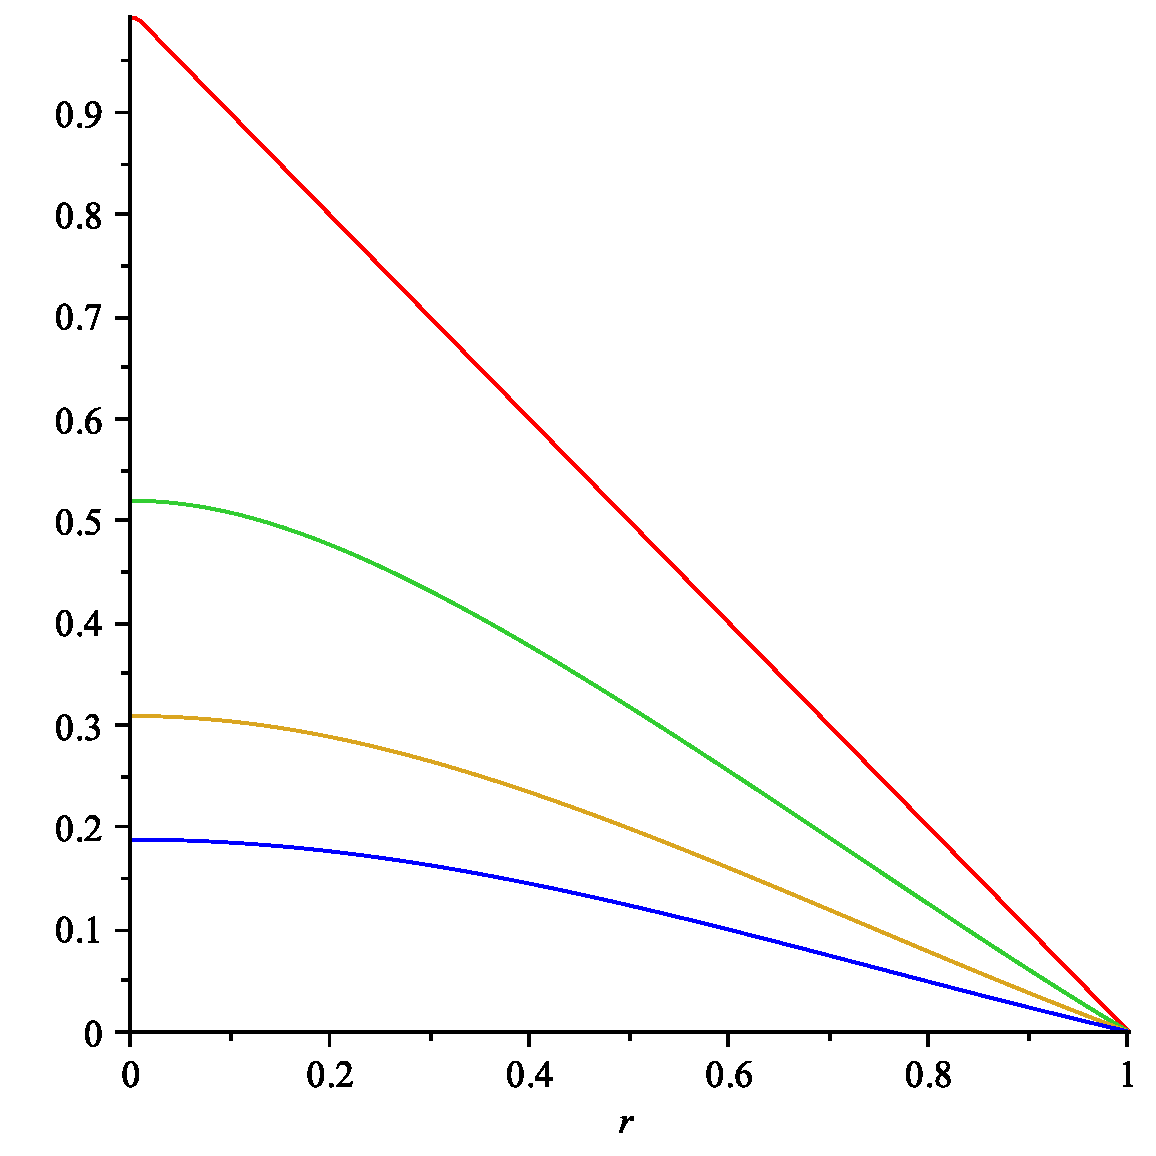
\includegraphics[width=4in]{heat-eqn-radially-sym-plot.pdf}
\end{center}

\end{example}






\section{General Circular Heat Equation}


The last section of this chapter focuses on the full heat equation in polar coordinates.  Recall that in section \ref{sect:heat:eqn:polar} that we derived (\ref{eq:heat:eqn:polar}),
%
\begin{align*}
\frac{1}{\kappa} \frac{\partial u}{\partial t} & = \frac{\partial^2 u}{\partial {r}^2}  + \frac{1}{r} \frac{\partial u}{\partial r}+ \frac{1}{r^2} \frac{\partial^2 u}{\partial {\theta}^2}
\end{align*}
Although there are numerous boundary conditions, let's take the conditions that on the edge of the region ($r=L$) that $u_r =0$, that is it is insulated.  When $r=0$, the center of the region, the temperature $u$ is finite.  These lead to the boundary conditions
%
\begin{align}
u_r(L,\theta,t) & = 0 & u(0,\theta,t) \text{~is finite} \label{eq:heat:eqn:polar:bc1}
\end{align}
and then since the region is continuous, we'll assume that
%
The boundary conditions on $\theta$ are different from what we've seen earlier.  There is no boundary, since the entire circular region is being studied.  Therefore, it is usually assumed that the temperature across the line $\theta=0$ (which is also $\theta=2\pi$) is continuous and smooth or 
\begin{align}
u(r,0,t) &= u(r,2\pi,t)&  u_{\theta}(r,0,t) & = u_{\theta} (r,0,t) \label{eq:heat:eqn:polar:bc2}
\end{align}
that is, the temperature at $\theta=0$ is identical to that at $\theta=2\pi$ and that the derivative match there as well.  


%
Again, as in previous chapters, we use separation of variables to solve this.  We'll make the assumption that $u = T(t) \Theta(\theta) R(r)$ and substitute this into (\ref{eq:heat:eqn:polar}) to get 
%
\begin{align*}
T'\Theta R &= R'' T\Theta+ \frac{1}{r} R' T \Theta + \frac{1}{r^2} R T \Theta'' &&\text{divide by $RT\Theta$} \\
\frac{T'\Theta R}{RT\Theta} &= \frac{R'' T\Theta+ \frac{1}{r} R' T \Theta + \frac{1}{r^2} R T \Theta'' }{RT\Theta} \\
\frac{T'}{T} & = \frac{R''}{R} + \frac{1}{r} \frac{R'}{R} + \frac{1}{r^2} \frac{\Theta''}{\Theta} 
\end{align*}
The left hand side only depends on $t$, therefore the right hand side must only depend on a constant.  If we let
%
\begin{align*}
\frac{\Theta''}{\Theta} & = -\lambda
\end{align*}
or
\begin{align}
\Theta'' + \lambda \Theta & = 0 \label{eq:heat:eqn:polar:theta}
\end{align}
and then the right hand side becomes:
% 
\begin{align}
\frac{R''}{R} + \frac{1}{r} \frac{R'}{R} - \frac{\lambda}{r^2}&  = \nu  \notag\intertext{mulitply through by $r^2$ and rearrange}
r^2 R'' + r R' + (r^2 \nu - \lambda) R & = 0, \label{eq:heat:eqn:polar:r}
\end{align}
which is Bessel's equation, (\ref{eq:bessel:eqn}).  Both (\ref{eq:heat:eqn:polar:theta}) and (\ref{eq:heat:eqn:polar:r}) with the boundary conditions in (\ref{eq:heat:eqn:polar:bc1}) and (\ref{eq:heat:eqn:polar:bc2}).  We now study those in the next section.  




\subsection{Sturm-Liouville Problems from the heat equation}

The first Sturm-Liouville problem from (\ref{eq:heat:eqn:polar:theta}) is
%
\begin{align*}
\Theta'' + \lambda \Theta & = 0 
\end{align*}
with boundary conditions $\Theta(0) = \Theta(2\pi)$ as well as $\Theta'(0) = \Theta'(2\pi)$, which arise from (\ref{eq:heat:eqn:polar:bc2}).  

As we've seen before in section \ref{sect:sturm:liouville}, this DE only has non trivial solution when $\lambda \geq 0$ and the solution is 
\begin{align*}
\Theta(\theta)  = c_1 \cos \sqrt{\lambda} \theta + c_2 \sin \sqrt{\lambda} \theta. 
\end{align*}
if $\lambda >0$ and $\Theta(\theta)=1$ if $\lambda=0$.  
%
Using the boundary condition above, 
\begin{align*}
\Theta (0) & = c_1 = \Theta(2\pi) = c_1 \cos 2\pi\sqrt{\lambda} + c_2 \sin 2\pi \sqrt{\lambda}
\end{align*}
which is satisfied when $\lambda = n^2$, for $n=1,2,3,\ldots$.  The derivative of $\Theta$ is
%
\begin{align*}
\Theta(\theta) & = -n c_1 \sin n \theta + n c_2 \cos n\theta
\end{align*}

The second boundary condition:
%
\begin{align*}
\Theta'(0) = n c_2 \cos (0) = \Theta'(2\pi) = -n c_1(0) + n c_2 \cos 2\pi n 
\end{align*}
which is satisfied.  Thus
%
\begin{align*}
\Theta(\theta) & = 1 & 
\Theta(\theta) &= \sin n \theta & & \text{and} & \Theta(\theta) & = \cos n \theta
\end{align*}
each satisfy the boundary condition.  

The next differential equation is
%
\begin{align*}
r^2 R''+ r R' + (r^2 \nu-n^2) R & = 0 
\end{align*}

The solution of this is
%
\begin{align*}
R(r) & = c_1 J_n(\sqrt{\nu} r) + c_2 Y_n(\sqrt{\nu} r)  
\end{align*}
and the boundary conditions are $R(0)$ is finite and $R(L)=0$.  The condition at $r=0$ sets $c_2=0$ and the other condition:
%
\begin{align*}
0 & = c_1 J_n(\sqrt{\nu}L) 
\end{align*}
results in
%
\begin{align*}
\sqrt{\nu} L & = \sigma_{n,i}
\end{align*}
where $\sigma_{n,i}$ is the $i$th root of $J_n(x)$.  Thus the eigenvalue is
%
\begin{align*}
\nu & = \frac{\sigma_{n,i}^2}{L^2} 
\end{align*}
and the eigenfunction is
%
\begin{align*}
J_n\biggl(\frac{\sigma_{n,i} r}{L} \biggr)
\end{align*}

The last DE is
%
\begin{align*}
\frac{1}{\kappa} \frac{T'}{T} & = \nu = \frac{\sigma_{n,i}^2}{L^2}
\end{align*}
of which the solution is: 
%
\begin{align*}
T & = e^{-\kappa (\sigma_{n,i}^2/L^2) t}  
\end{align*}


\begin{align*}
u_{0,i} & = J_0\biggl(\frac{\sigma_{0,i} r}{L} \biggr) e^{-\kappa (\sigma_{0,i}^2/L^2) t}  \\
u_{n,i} & = R_{n,i}(r) \Theta_n T_{n,i} \\
& = J_n\biggl(\frac{\sigma_{n,i} r}{L} \biggr) (a_n \cos n \theta + b_n \sin \theta) e^{-\kappa (\sigma_{n,i}^2/L^2) t}  
\end{align*}
and using the principle of superposition the full solution is:

%
\begin{align*}
u(r,\theta,t) & = \sum_{i=1}^{\infty} a_0 J_0\biggl(\frac{\sigma_{0,i} r}{L} \biggr) e^{-\kappa (\sigma_{0,i}^2/L^2) t}  + \\
& \qquad \sum_{i=1}^{\infty}  \sum_{n=1}^{\infty} J_n\biggl(\frac{\sigma_{n,i} r}{L} \biggr) ( a_n \cos n \theta + b_n \sin \theta) e^{-\kappa (\sigma_{n,i}^2/L^2) t}  
\end{align*}

Finding the coefficients.  In this case we use the initial condition that 
%
\begin{align*}
u(r,\theta,0) & = f(r,\theta) 
\end{align*}
and substituting into the solution:
%
\begin{align*}
f(r,\theta) & = \sum_{i=1}^{\infty} a_0 J_0\biggl(\frac{\sigma_{0,i} r}{L} \biggr) + 
 \sum_{i=1}^{\infty}  \sum_{n=1}^{\infty} J_n\biggl(\frac{\sigma_{n,i} r}{L} \biggr) ( a_n \cos n \theta + b_n \sin \theta)
 \end{align*}
The coefficients are:
%
\begin{align*}
a_{0,i} & = \frac{\int_0^L \int_0^{2\pi} r f(r,\theta) J_0(\sigma_{0,i} r/L) \,d\theta \, dr}
{2\pi \int_0^L  r J_0(\sigma_{0,i} r/L)^2  \, dr}\\
a_{n,i} & = \frac{\int_0^L \int_0^{2\pi} r f(r,\theta) J_n(\sigma_{n,i} r/L)\cos n\theta \,d\theta \, dr}
{\pi \int_0^L  r J_n(\sigma_{0,i} r/L)^2  \, dr} \\
b_{n,i} & = \frac{\int_0^L \int_0^{2\pi} r f(r,\theta) J_n(\sigma_{n,i} r/L)\sin n\theta \,d\theta \, dr}
{\pi \int_0^L  r J_n(\sigma_{0,i} r/L)^2  \, dr}
\end{align*}


\begin{example}
Solve the equation above when $f(r,\theta) = J_1(\sigma_{1,1} r) \sin \theta$.  Use $\kappa=0.04$ and $L=1$.   

\solution

Again, we just need to compute the coefficients above.  Use can either use Maple or make a symmetry argument to see that
%
\begin{align*}
a_{0,i} & = 0 \\
a_{n,i} & = 0 \\
b_{1,1} & = 1 \\
a_{n,i} & = 0 \qquad n \neq 1, i \neq 1.  
\end{align*}

So the solution is 
% 
\begin{align*}
u(r, \theta,t) & = J_1(\sigma_{1,1} r) \sin \theta e^{-0.04 \sigma{1,1}^2 t} 
\end{align*}

\end{example}


% !TEX root = applied-math.tex


\chapter{Differential Equations on \texorpdfstring{$\mathbb{R}$}{the real number line} and the Fourier Transform}
 


\section{The Fourier Transform}

From above, we can write the Fourier Series of $f(x)$ on $[-L/2,L/2]$ as
%
\begin{align*}
f(x) & = \sum_{n=-\infty}^{\infty} c_n e^{i n \omega_0 x} \intertext{where}
c_n & = \frac{1}{L} \int_{-L/2}^{L/2} f(x) e^{-in\omega_0 x} \, dx 
\end{align*}

where $\omega_0=2\pi/L$ and $\omega_n=n\omega_0$ and let
%
\begin{align*}
\Delta \omega = \omega_{n+1}-\omega_n = \frac{2\pi}{L} 
\end{align*}

The series can be written:
%
\begin{align*}
f(x) & = \sum_{n=-\infty}^{\infty} \biggl[\frac{1}{2\pi} \int_{-L/2}^{L/2} f(x) e^{-i\omega_n x} \, dx \biggr] e^{i \omega_n x} \Delta \omega
\end{align*}
and letting $L \rightarrow \infty$ or $\Delta \omega \rightarrow 0$, we get:
%
\begin{align*}
f(x) & = \int_{-\infty}^{\infty}  \biggl[\frac{1}{2\pi} \int_{-\infty}^{\infty} f(x) e^{-i\omega_n x} \, dx \biggr] e^{i \omega x} d \omega
\end{align*}
which can be written as follows:

\begin{Boxed}
The \textbf{Fourier Transform} of $f$ is :
\begin{align*}
\hat{f}(\omega) & = \frac{1}{\sqrt{2\pi}} \int_{-\infty}^{\infty} f(x) e^{-i \omega x} \, dx 
\end{align*}
and using this, the function $f(x)$ can be written:
\begin{align*}
f(x) & = \frac{1}{\sqrt{2\pi}} \int_{-\infty}^{\infty} \hat{f}(x) e^{i \omega x} \, d\omega 
\end{align*}
Note: not all functions have a Fourier Transform. If the integral is defined (and converges), then the transform exists. 
\end{Boxed} 

(discussion of function space versus frequency space). 

\begin{example}
Find the Fourier Transform of 
%
\begin{align*}
f(x) = \begin{cases}
e^{-ax} & x \geq 0 \\
0 & \text{otherwise} 
\end{cases}
\end{align*}

\solution

\begin{align*}
\hat{f}(\omega) & =\frac{1}{\sqrt{2\pi}}\int_{-\infty}^{\infty} f(x)  e^{-i \omega x} \, dx \\
& =\frac{1}{\sqrt{2\pi}}\int_{0}^{\infty} e^{-ax} e^{-i\omega x} \, dx \\
& =\frac{1}{\sqrt{2\pi}} \int_0^{\infty} e^{-(a+i\omega) x} \, dx \\
& = \frac{1}{\sqrt{2\pi}} \frac{-1}{a+i\omega} e^{-(a + i \omega)x} \biggr\vert_0^{\infty} =\frac{1}{\sqrt{2\pi}} \frac{1}{a+i\omega} = \frac{1}{\sqrt{2\pi} }\frac{a-i\omega}{a^2+\omega^2} 
\end{align*}

\end{example}

\subsection{Even and Odd Functions and Fourier Transforms}

\begin{Boxed}
if $f(x)$ is an even function then the Fourier Transform can be written:
%
\begin{align*}
f(x) & = \int_{-\infty}^{\infty} \hat{f}(x) e^{i \omega x} \, d\omega \intertext{where}
\hat{f} (x) & = \frac{1}{2\pi} 
\end{align*}


\end{Boxed}

\begin{example}
Fourier Transform of the function
%
\begin{align*}
f(x) & = \begin{cases}
1 & | x| \leq 1 \\
0 & otherwise
\end{cases}
\end{align*}

\solution

The Fourier Transform is:
%
\begin{align*}
\hat{f}(\omega) & = \frac{1}{\sqrt{2\pi}} \int_{-\infty}^{\infty} f(x) e^{-i\omega x} \, dx \\
& = \frac{1}{\sqrt{2\pi}} \int_{-1}^{1} e^{-i\omega x} \, dx \\
& = \frac{1}{\sqrt{2\pi}} \frac{1}{-i \omega}  e^{-i\omega x} \biggr\vert_{-1}^1  \\
& = \frac{1}{\sqrt{2\pi}} \biggl( \frac{e^{-i\omega}}{-i \omega } + \frac{e^{i\omega}}{i \omega} \biggr) \\
& = \frac{1}{\sqrt{2\pi}} \frac{2 \sin \omega}{\omega}  
\end{align*}

Also, 
%
\begin{align*}
f(x) & = \frac{1}{\sqrt{2\pi}} \int_{-\infty}^{\infty} \hat{f}(\omega) e^{i \omega x} \, d\omega \\
& = \frac{1}{2\pi} \int_{-\infty}^{\infty} \frac{2 \sin \omega}{\omega} e^{i \omega x} \, d \omega 
\end{align*}

Since $f(0)=1$ (from the original definition of the function), this means that
%
\begin{align*}
1 & = \frac{1}{\pi} \int_{-\infty}^{\infty}\frac{\sin \omega}{\omega} \, d\omega  \intertext{or}
\pi & = \int_{-\infty}^{\infty}\frac{\sin \omega}{\omega} \, d\omega 
\end{align*}
since $\frac{\sin \omega}{\omega}$ is an even function we can write:
%
\begin{align*}
\frac{\pi}{2} & = \int_{0}^{\infty} \frac{\sin \omega}{\omega} \, d\omega
\end{align*}

An important function is that on the right side 
%
\begin{align*}
\mbox{Si}(u) & = \int_{0}^u \frac{\sin \omega}{\omega} \, d\omega 
\end{align*}



\end{example}


\subsection{Physical Interpretation of the Fourier Transform}

The Fourier Transform of a function $f(x)$ is a function that lists all of its frequencies, often called the \textbf{spectral representation}.  The name come from understanding light in terms of its frequencies (colors) and many analyses in physics and chemistry are easier to do in term of the spectrum 

\begin{definition}
The \textbf{total energy} is 
%
\begin{align*}
\int_{-\infty}^{\infty} | \hat{f}(\omega)|^2 \, d\omega
\end{align*}
\end{definition}


\subsection{Properties of the Fourier Transform}

\begin{theorem}[Linearity]
The Fourier Transform is \emph{linear}; that is, for any pair of functions $f(x)$ and $g(x)$ whose Fourier transforms exist and any constants $a$ and $b$, then
%
\begin{align*}
{\cal F}(af+bg) &  = a {\cal F}(f) + b {\cal F}(g)  
\end{align*}
\end{theorem}

\begin{proof}
\begin{align*}
{\cal F}(af+bg) & = \frac{1}{\sqrt{2\pi}} \int_{-\infty}^{\infty} (a f(x) + b g(x)) \, dx \\
& = a \frac{1}{\sqrt{2\pi}} \int_{-\infty}^{\infty} f(x) \, dx + b \frac{1}{\sqrt{2\pi}} \int_{-\infty}^{\infty} g(x) \, dx \\
& = a {\cal F}(f) + b {\cal F}(g) 
\end{align*}
\end{proof}


\begin{theorem}[Derivatives]
Let $f(x)$ be a continuous on the $x$-axis and $f(x) \rightarrow 0$ as $|x| \rightarrow \infty$.  Furthermore, let $f'(x)$ be absolutely integrable on the $x$-axis.  Then 
\begin{align*}
{\cal F}\bigl\{f'(x) \bigr\} & = i \omega {\cal F} \bigl\{ f(x) \bigr\} 
\end{align*}

\end{theorem}
\begin{proof}
\begin{align*}
{\cal F} \bigl\{ f'(x) \bigr\} & = \frac{1}{\sqrt{2\pi}} \int_{-\infty}^{\infty} f'(x) e^{-i \omega x} \, dx  \intertext{integrate by parts} 
& = \frac{1}{\sqrt{2\pi}} \biggl( f(x) e^{-i \omega x} \biggr\vert_{-\infty}^{\infty} - (-i\omega) \int_{-\infty}^{\infty} f(x) e^{-i \omega x} \, dx \biggr) \intertext{since $f(x) \rightarrow 0$ as $|x|\rightarrow \infty$} 
& = \frac{1}{\sqrt{2\pi}} i\omega {\cal F} \bigl\{ f(x) \bigr\} 
\end{align*}
\end{proof}




\section{Solving the Heat Equation using Fourier Transform}

Now we solve:
%
\begin{align*}
\frac{1}{\kappa}\frac{\partial u}{\partial t} & = \frac{\partial^2 u}{\partial {x}^2} 
\end{align*}
if $-\infty < x < \infty$ and $u(x,0)=f(x)$.  

Let $\hat{u}(\omega,t)$ be the Fourier Transform of $u(x,t)$.  Taking the Fourier Transform of the PDE above:
%
\begin{align*}
\frac{1}{\kappa} \frac{\partial \hat{u}}{\partial t} & = \frac{\partial^2 \hat{u}}{\partial {x}^2} 
\end{align*}
and using the derivative of the Fourier Transform:
\begin{align*}
\frac{1}{\kappa} \frac{\partial U}{\partial t} & = (i\omega)^2 \hat{u} = -\omega^2 \hat{u} 
\end{align*}
and solving this we get:
%
\begin{align*}
\hat{u}(\omega,t) & = A(\omega) e^{-\kappa \omega^2 t}   
\end{align*}

If we take the Fourier Transform of the initial condition:
%
\begin{align*}
\hat{u}(\omega,0) & = {\cal F}\{f(x)\} = \hat{f}(\omega)
\end{align*}

and then evaluate the transformed solution to get:
%
\begin{align*}
\hat{u}(\omega,0) & = A(\omega) \intertext{so}
\hat{u}(\omega,t) & = \hat{f}(\omega) e^{-\kappa \omega^2 t} 
\end{align*}
and lastly, we take the inverse transform:
%
\begin{align*}
u(x,t) & = \frac{1}{\sqrt{2\pi}} \int_{-\infty}^{\infty} \hat{f}(\omega) e^{-\kappa \omega^2 t}  e^{i\omega x} \, d\omega 
\end{align*}


\begin{example}
Solve the Heat equation on the real line if the initial condition is
%
\begin{align*}
f(x) & = \begin{cases}
1 & |x| \leq 1 \\
0 & \text{otherwise}
\end{cases}
\end{align*}

\solution

From above
%
\begin{align*}
\hat{f}(\omega) & = \frac{1}{\sqrt{2\pi}} \frac{\sin \omega}{\omega}
\end{align*}
so the solution is:
%
\begin{align*}
u(x,t) & = \frac{1}{\sqrt{2\pi}}\int_{-\infty}^{\infty}  \frac{1}{\sqrt{2\pi}} \frac{\sin \omega}{\omega} e^{-\kappa \omega^2 t + i \omega x} \, d\omega 
\end{align*}

\end{example}







%\appendix

%\input{solutions}

\printindex
\end{document}